% Generated visual comparison of main.tex and main_revised.tex; base repository revision 6ccb62a22386d4b58185818276b578fe287de531.
% Compile diff.tex from this repository using pdfLaTeX and BibTeX.
% Text uses latexdiff; complete original/revised floats preserve their respective values and artwork.
% Source SHA256: {"main.tex": "b0b9547982490227a287f4f7301158663486f98b8e56e31edf82251abacfda3a", "main_revised.tex": "2ba1c17b55b3da19e49ed87a26663f2a74ac5a9455959069fd6dff1d4ebbad08"}
\documentclass[letterpaper,journal]{IEEEtran}
%DIF LATEXDIFF DIFFERENCE FILE
%DIF DEL main.tex (original)
%DIF ADD main_revised.tex (revised)
\usepackage{amsmath,amsfonts,amssymb}
\usepackage{array,graphicx,xcolor,booktabs,tabularx}
\usepackage{url}

\usepackage[nocompress]{cite}
\hyphenation{op-tical net-works semi-conduc-tor IEEE-Xplore}
\newcommand{\agent}[1]{{\bf\color{red}: #1}}
%DIF PREAMBLE EXTENSION ADDED BY LATEXDIFF
%DIF UNDERLINE PREAMBLE %DIF PREAMBLE
\RequirePackage[normalem]{ulem} %DIF PREAMBLE
\RequirePackage{color}\definecolor{RED}{rgb}{1,0,0}\definecolor{BLUE}{rgb}{0,0,1} %DIF PREAMBLE
\providecommand{\DIFadd}[1]{{\protect\color{blue}\uwave{#1}}} %DIF PREAMBLE
\providecommand{\DIFdel}[1]{{\protect\color{red}\sout{#1}}}                      %DIF PREAMBLE
%DIF SAFE PREAMBLE %DIF PREAMBLE
\providecommand{\DIFaddbegin}{} %DIF PREAMBLE
\providecommand{\DIFaddend}{} %DIF PREAMBLE
\providecommand{\DIFdelbegin}{} %DIF PREAMBLE
\providecommand{\DIFdelend}{} %DIF PREAMBLE
\providecommand{\DIFmodbegin}{} %DIF PREAMBLE
\providecommand{\DIFmodend}{} %DIF PREAMBLE
%DIF FLOATSAFE PREAMBLE %DIF PREAMBLE
\providecommand{\DIFaddFL}[1]{\DIFadd{#1}} %DIF PREAMBLE
\providecommand{\DIFdelFL}[1]{\DIFdel{#1}} %DIF PREAMBLE
\providecommand{\DIFaddbeginFL}{} %DIF PREAMBLE
\providecommand{\DIFaddendFL}{} %DIF PREAMBLE
\providecommand{\DIFdelbeginFL}{} %DIF PREAMBLE
\providecommand{\DIFdelendFL}{} %DIF PREAMBLE
%DIF COLORLISTINGS PREAMBLE %DIF PREAMBLE
\RequirePackage{listings} %DIF PREAMBLE
\RequirePackage{color} %DIF PREAMBLE
\lstdefinelanguage{DIFcode}{ %DIF PREAMBLE
%DIF DIFCODE_UNDERLINE %DIF PREAMBLE
  moredelim=[il][\color{red}\sout]{\%DIF\ <\ }, %DIF PREAMBLE
  moredelim=[il][\color{blue}\uwave]{\%DIF\ >\ } %DIF PREAMBLE
} %DIF PREAMBLE
\lstdefinestyle{DIFverbatimstyle}{ %DIF PREAMBLE
	language=DIFcode, %DIF PREAMBLE
	basicstyle=\ttfamily, %DIF PREAMBLE
	columns=fullflexible, %DIF PREAMBLE
	keepspaces=true %DIF PREAMBLE
} %DIF PREAMBLE
\lstnewenvironment{DIFverbatim}{\lstset{style=DIFverbatimstyle}}{} %DIF PREAMBLE
\lstnewenvironment{DIFverbatim*}{\lstset{style=DIFverbatimstyle,showspaces=true}}{} %DIF PREAMBLE
%DIF END PREAMBLE EXTENSION ADDED BY LATEXDIFF


% Review-only support; original manuscript files are not modified.
\usepackage{adjustbox}
\newlength{\DiffColumnWidth}
\AtBeginDocument{\setlength{\DiffColumnWidth}{\columnwidth}}
\newcommand{\DiffOriginalCaption}[1]{\par\smallskip\noindent{\footnotesize #1\par}}

\begin{document}
\title{Nonintrusive \DIFdelbegin \DIFdel{Cross-Motor }\DIFdelend Detection\DIFaddbegin \DIFadd{, Localization, }\DIFaddend and Severity Assessment of False-Data-Injection Attacks in Heterogeneous \DIFdelbegin \DIFdel{Inverter-Fed Drives
}\DIFdelend \DIFaddbegin \DIFadd{Motor-Drive Systems
}\DIFaddend }

\author{
    Abolfazl Najar, He Yang, Jin Ye,~\IEEEmembership{Senior Member,~IEEE},  Ping Ma and WenZhan Song,~\IEEEmembership{Senior Member,~IEEE}

    \thanks{Abolfazl Najar, He Yang, Jin Ye, and WenZhan Song are with the College of Engineering, University of Georgia, Athens, GA 30602, USA (e-mail: najar@uga.edu; heyang95@uga.edu; jin.ye@uga.edu; wsong@uga.edu).}

    \DIFdelbegin %DIFDELCMD < \thanks{Ping Ma are with the Department of Statistics, University of Georgia, Athens, GA 30602, USA (e-mail: pingma@uga.edu).}
%DIFDELCMD <     %%%
\DIFdelend \DIFaddbegin \thanks{Ping Ma \DIFdel{are}\DIFadd{is} with the Department of Statistics, University of Georgia, Athens, GA 30602, USA (e-mail: pingma@uga.edu).}
\DIFaddend

    \thanks{Corresponding author: Jin Ye (e-mail: jin.ye@uga.edu).}

}

\maketitle

\begin{center}
\fbox{\parbox{0.94\columnwidth}{\small
\textbf{Comparison: main.tex $\rightarrow$ main\_revised.tex}\\[3pt]
\DIFadd{Blue underlined text is added or revised.}\\
\DIFdel{Red struck-out text is removed.}\\[3pt]
Unmarked text is unchanged. Tables and figures are paired as complete ORIGINAL and REVISED blocks (left/right or top/bottom). Cross-references follow the revised numbering; deleted references to removed floats retain their original numbers. Formatting-only changes and commented-out source text are not marked word by word.
}}
\end{center}


\begin{abstract}
\DIFdelbegin %DIFDELCMD <

%DIFDELCMD < %%%
\DIFdel{This paper presents an experimentally validated method for detecting false-data-injection attacks (FDIA) and estimating attack severity in heterogeneous motor-drive systemsusing measurements acquired either at the motor terminals or at the point-of-common-coupling.
The method extracts multi-scale features from variable-size windows and uses an InceptionTime model for binary attack detection and four-level severity classification.
Experiments on a two-branch platform containing one }\DIFdelend \DIFaddbegin \DIFadd{False-data-injection attacks on current feedback can compromise the operation of inverter-fed motor drives. In heterogeneous multi-motor systems, installing monitoring sensors at each motor increases instrumentation requirements, while measurements at the shared point of common coupling (PCC) combine responses from different drives. This aggregation makes it difficult to detect small attacks, identify the affected motor, and distinguish injected-bias levels, limiting the use of centralized monitoring.
This paper addresses these tasks using PCC voltage and current measurements, with motor-terminal currents evaluated separately as a reference. Multiscale electrical features and task-specific InceptionTime classifiers are validated on a platform containing an }\DIFaddend alternating current induction motor \DIFdelbegin \DIFdel{(ACIM) drive and one }\DIFdelend \DIFaddbegin \DIFadd{and a }\DIFaddend permanent magnet synchronous motor\DIFdelbegin \DIFdel{(PMSM) drive show that motor-side sensing yields the strongest class separability, while point-of-common-coupling (PCC) sensing remains attractive for nonintrusive deployment. In the mixed-domain setting, binary detection reaches 98.89\% accuracy with motor-side data and 89.44\% accuracy with PCC data. For four-class severity assessment, the motor-side stream achieves 98.68\% accuracy, while the PCC stream achieves 84.17\% accuracy. Among the evaluated deep-learning and classical machine-learning baselines, the proposed method achieved the best PCC-side performance for both binary detection and four-level severity assessment.
For the PCC-side tasks, the proposed method outperformed the evaluated baselines, achieving 89.44\% accuracy for binary detection and 84.17\% accuracy for four-level severity classification , compared with the best baseline accuracies of 86.45\% and 83.42\% , respectively. In }\DIFdelend \DIFaddbegin \DIFadd{. The evaluation keeps complete recordings and their episodes separate across training, validation, and test sets and examines }\DIFaddend cross-motor \DIFdelbegin \DIFdel{experiments, few-shot }\DIFdelend \DIFaddbegin \DIFadd{adaptation and selective feature computation.
PCC measurements achieve mean accuracies of 80.78\% for attack detection and 74.32\% for joint detection and motor localization, supporting monitoring without dedicated motor-terminal sensors. Severity classification remains more challenging, with 61.00\% accuracy. Target-domain }\DIFaddend fine-tuning \DIFdelbegin \DIFdel{improved transferperformance, especially in the PMSM-to-ACIM direction}\DIFdelend \DIFaddbegin \DIFadd{improves cross-motor transfer, while feature pruning increases the processing rate by 85.18\% at 80.29\% balanced detection accuracy}\DIFaddend . These results \DIFdelbegin \DIFdel{indicate that PCC-based FDIA monitoring is promising }\DIFdelend \DIFaddbegin \DIFadd{establish the feasibility and current limitations of PCC monitoring }\DIFaddend on the tested \DIFdelbegin \DIFdel{ACIM/PMSM platform.
}%DIFDELCMD <

%DIFDELCMD < %%%
\DIFdelend \DIFaddbegin \DIFadd{heterogeneous drive platform.
}\DIFaddend \end{abstract}

\begin{IEEEkeywords}
False-data-injection attack, point of common coupling, inverter-fed motor drives, heterogeneous motor drives, nonintrusive monitoring, cross-motor adaptation, severity assessment, cyber-physical security
\end{IEEEkeywords}

\section{Introduction}
\label{sec:introduction}

\DIFdelbegin %DIFDELCMD < \IEEEPARstart{F}{DIA} %%%
\DIFdelend \DIFaddbegin \IEEEPARstart{F}{alse}\DIFadd{-data-injection attack (FDIA) }\DIFaddend detection and severity assessment are important in networked motor-drive systems, where manipulated sensor feedback can degrade control performance and cause unsafe operation~\cite{Ghaderi2021A}. Increasing drive connectivity makes timely detection of sensor-oriented \DIFdelbegin \DIFdel{cyber attacks }\DIFdelend \DIFaddbegin \DIFadd{cyberattacks }\DIFaddend essential for resilient operation~\cite{Yang2022Fast,Yang2024Enhanced}.
Current signals are attractive for FDIA monitoring because they are easy to acquire, strongly coupled to electromechanical dynamics, and have been shown to reveal sensor-integrity attacks in motor drives~\cite{7944701, YangVulnerability}. However, most existing studies emphasize terminal-side sensing, operate on a single machine domain, or assume sufficient labeled data for supervised training. These assumptions limit practicality in heterogeneous deployments where different motor types, sensing locations, and data availability constraints all affect performance.
Motivated by these limitations, this work experimentally evaluates FDIA detection in a heterogeneous motor-drive setting involving both \DIFdelbegin \DIFdel{ACIM and PMSM }\DIFdelend \DIFaddbegin \DIFadd{alternating current induction motor (ACIM) and permanent magnet synchronous motor (PMSM) }\DIFaddend domains. The study evaluates binary detection \DIFaddbegin \DIFadd{(}\texttt{\DIFadd{fdia2}}\DIFadd{)}\DIFaddend , four-level severity assessment \DIFaddbegin \DIFadd{(}\texttt{\DIFadd{severity4}}\DIFadd{)}\DIFaddend , cross-domain transfer, and deployment feasibility. The framework combines low-frequency (LF), high-frequency (HF), and time-domain (TD) \DIFdelbegin \DIFdel{current }\DIFdelend \DIFaddbegin \DIFadd{electrical }\DIFaddend features with an InceptionTime classifier, and compares motor-terminal and \DIFdelbegin \DIFdel{PCC sensing.
}\DIFdelend \DIFaddbegin \DIFadd{point of common coupling (PCC) sensing. A three-class classifier (}\texttt{\DIFadd{fdia3}}\DIFadd{) additionally distinguishes normal operation, an ACIM attack, and a PMSM attack.
}\DIFaddend

\subsection{Challenges at PCC in Heterogeneous Multi-Motor Systems}
\label{sec:pcc_challenges}

From a deployment perspective, motor-terminal measurements provide cleaner machine-specific signatures, whereas PCC measurements are more scalable and \DIFdelbegin \DIFdel{non-intrusive}\DIFdelend \DIFaddbegin \DIFadd{nonintrusive}\DIFaddend . PCC sensing is attractive because it avoids direct motor-terminal instrumentation and is compatible with shared electrical infrastructure~\cite{7271086}. However, PCC currents are affected by converter harmonics, network interactions, and load aggregation. Consequently, PCC attack signatures are weaker and less separable than motor-terminal signatures~\cite{10005067}.
The problem becomes more difficult in heterogeneous multi-motor settings. ACIM and PMSM systems exhibit different current characteristics even under the same attack framework, which introduces a substantial domain shift between source and target deployments. Consequently, a detector trained on one motor family may generalize poorly to the other unless explicit adaptation is used. Therefore, this study evaluates in-domain performance, source-only transfer, few-shot adaptation, and transfer-direction asymmetry.
\subsection{Contributions}
\label{sec:contributions}
The main contributions of this work are as follows:

\begin{itemize}
\item \textbf{\DIFdelbegin \DIFdel{Developed}%DIFDELCMD < \MBLOCKRIGHTBRACE %%%
\DIFdel{and validated a PCC-based FDIA monitoring framework for heterogeneous inverter-fed drives, showing that PCC sensing supports useful binary detectionand coarse four-level }\DIFdelend \DIFaddbegin \DIFadd{Nonintrusive FDIA monitoring in heterogeneous motor drives:}} \DIFadd{We develop and experimentally validate a PCC monitoring framework that combines LF, HF, and TD electrical features with task-specific InceptionTime classifiers, enabling attack detection, localization to the ACIM or PMSM, and injected-bias }\DIFaddend severity assessment without \DIFdelbegin \DIFdel{direct }\DIFdelend \DIFaddbegin \DIFadd{dedicated }\DIFaddend motor-terminal \DIFdelbegin \DIFdel{instrumentation}\DIFdelend \DIFaddbegin \DIFadd{sensors}\DIFaddend .
\item \textbf{\DIFdelbegin \DIFdel{Constructed}%DIFDELCMD < \MBLOCKRIGHTBRACE %%%
\DIFdel{a multi-scale LF/HF/TD current-feature representation and showed that it improves PCC-side separability under harmonic distortion and signal aggregation, while also enabling stronger motor-side performance}\DIFdelend \DIFaddbegin \DIFadd{Cross-motor adaptation with limited labeled data:}} \DIFadd{We evaluate a supervised adaptation strategy that fine-tunes a source-trained detector using complete labeled target-domain episodes, enabling a PCC balanced-accuracy gain of 21.43 percentage points for PMSM-to-ACIM transfer with a nominal 1\% target-episode budget}\DIFaddend .
\item \textbf{\DIFdelbegin \DIFdel{Provided}%DIFDELCMD < \MBLOCKRIGHTBRACE %%%
\DIFdel{a cross-motor evaluation across ACIM and PMSM domains, including source-only transfer, few-shot target-domain adaptation, and latency/pruning analysis, showing both the limits of direct transfer and the practical gains from lightweight adaptation}\DIFdelend \DIFaddbegin \DIFadd{Computationally efficient PCC monitoring:}} \DIFadd{We develop a reduced-feature inference pipeline that selects features using validation-set permutation importance and computes only the selected features and their required intermediate quantities, enabling an 85.18\% processing speedup with 18 of 74 features while retaining 80.29\% mean detection balanced accuracy}\DIFaddend .
\end{itemize}

The remainder of this paper is organized as follows: Section~\ref{sec:relatedWorks} reviews related literature. Section~\ref{sec:system_data} describes the physical system and dataset construction, while Section~\ref{sec:method} details the proposed FDIA detection framework and feature pipeline. Experimental results and cross-domain adaptations are reported in Section~\ref{sec:results}. Section~\ref{sec:realtime} analyzes real-time deployment and latency, followed by a discussion of tradeoffs in Section~\ref{sec:discussion}. Section~\ref{sec:conclusion} concludes the paper.

\section{Related Work}
\label{sec:relatedWorks}

FDIA detection has been studied extensively in smart grids and broader cyber-physical systems (CPS), but the assumptions in that literature do not transfer cleanly to inverter-fed motor drives. Many grid- and CPS-oriented approaches rely on state estimation, observer-based detection, invariant analysis, adaptive neuro-fuzzy models, or graph-based learning~\cite{7438916,basati2022fdi,nath2022quickest,beg2017fdia,sargolzaei2020fdia,10016905}. These studies demonstrate strong FDIA-detection capability at the system level, but they are generally not designed for drive-level current monitoring or for deployment at a shared \DIFdelbegin \DIFdel{point of common coupling (PCC)}\DIFdelend \DIFaddbegin \DIFadd{PCC}\DIFaddend .

Motor-drive-specific studies \DIFdelbegin \DIFdel{are more closely related to the present work. Prior work has }\DIFdelend \DIFaddbegin \DIFadd{have }\DIFaddend shown that current signals can support effective FDIA detection in electric-drive systems and that transfer learning can improve performance when labeled data are limited~\cite{Yang2022Fast,Yang2024Enhanced}. Related industrial-IoT monitoring studies have also considered cyber-detection in machine-monitoring settings~\cite{423563247547}. However, these studies mainly rely on motor-terminal sensing, single-motor settings, or closely related operating domains, and therefore provide limited evidence for heterogeneous cross-motor transfer.





The main gap is not FDIA detection in general, which has been widely studied in smart grids and cyber-physical systems, but nonintrusive PCC-based monitoring for heterogeneous inverter-fed motor-drive systems. In particular, the existing literature does not clearly establish: 1) how PCC sensing compares with motor-side sensing for low-severity current-feedback FDIAs, 2) whether PCC measurements support reliable multi-level severity assessment rather than only binary detection, given that attack signatures become weaker and less separable under signal aggregation and harmonic distortion, and 3) how detection performance transfers between heterogeneous ACIM and PMSM domains when labeled target-domain data are limited. This work addresses these three questions experimentally on a shared ACIM/PMSM platform using multi-scale features, in-domain evaluation, source-only cross-domain transfer, and few-shot target-domain adaptation.

\section{System and Data}
\DIFaddbegin

\DIFaddend \label{sec:system_data}
\DIFdelbegin \subsection{\DIFdel{Experimental Platform: ACIM/PMSM and PCC Sensing}}
%DIFAUXCMD
\addtocounter{subsection}{-1}%DIFAUXCMD
%DIFDELCMD < \label{sec:experimental_platform}
%DIFDELCMD < %%%
\DIFdelend

\DIFdelbegin \DIFdel{Fig.~\ref{fig:system_schematic} illustrates the overall setup, including the shared PCC, the two drive branches, the ACIM and PMSM loads, the sensing locations, and the FDIA injection points in the control/feedback paths. }\DIFdelend The experimental platform consists of a heterogeneous two-motor industrial setup including one ACIM branch and one PMSM branch. Both branches are supplied from a common upstream electrical interface, enabling measurements at the PCC in addition to motor-side measurements. This setup enables comparison of motor-terminal and PCC sensing under heterogeneous ACIM/PMSM dynamics.
\DIFdelbegin \DIFdel{A total of }\DIFdelend \DIFaddbegin \subsection{\DIFadd{Experimental Platform: ACIM/PMSM and PCC Sensing}}
\label{sec:experimental_platform}

\DIFadd{Fig.~\ref{fig:system_schematic} illustrates the overall setup, including the shared PCC, the two drive branches, the ACIM and PMSM loads, the sensing locations, and the FDIA injection points in the control/feedback paths.
The dataset contains }\DIFaddend 540 \DIFdelbegin \DIFdel{unique FDIA cases were collected, including 270 ACIM cases and }\DIFdelend \DIFaddbegin \DIFadd{scheduled attack episodes (}\DIFaddend 270 \DIFdelbegin \DIFdel{PMSM cases}\DIFdelend \DIFaddbegin \DIFadd{for each motor), formed by repeating 30 bias patterns over nine speed/load combinations per motor. All episodes were acquired on the same two-motor platform. Both motors operated throughout: only the ACIM was attacked in ACIM-labeled recordings, and only the PMSM was attacked in PMSM-labeled recordings. Both motors were attack-free during normal intervals}\DIFaddend . The experiments cover three speed operating points, namely 900, 1100, and 1300 \DIFdelbegin \DIFdel{rpm}\DIFdelend \DIFaddbegin \DIFadd{RPM}\DIFaddend .

Two measurement streams were used throughout this study. The first stream corresponds to motor-side measurements, referred to as \emph{motor} in the remainder of the paper. The second stream corresponds to PCC-side measurements, referred to as \emph{PCC}. The PCC stream is the primary deployment-oriented sensing location because it avoids dedicated sensors at each machine.
\DIFdelbegin \DIFdel{The measured signals and channel counts associated with the motor-side and PCC-side streams are summarized in Table~\ref{tab:measurement_streams}.
}\DIFdelend \DIFaddbegin




\begin{figure*}[p]
\centering
\begin{adjustbox}{max width=\textwidth,max totalheight=0.87\textheight}
\begin{minipage}{\textwidth}
\centering
% Complete old block: fig:system_schematic
\begin{minipage}[t]{\textwidth}
\centering
\textcolor{red}{\textbf{ORIGINAL --- Figure 1 (main.tex)}}\par\smallskip

    \centering
    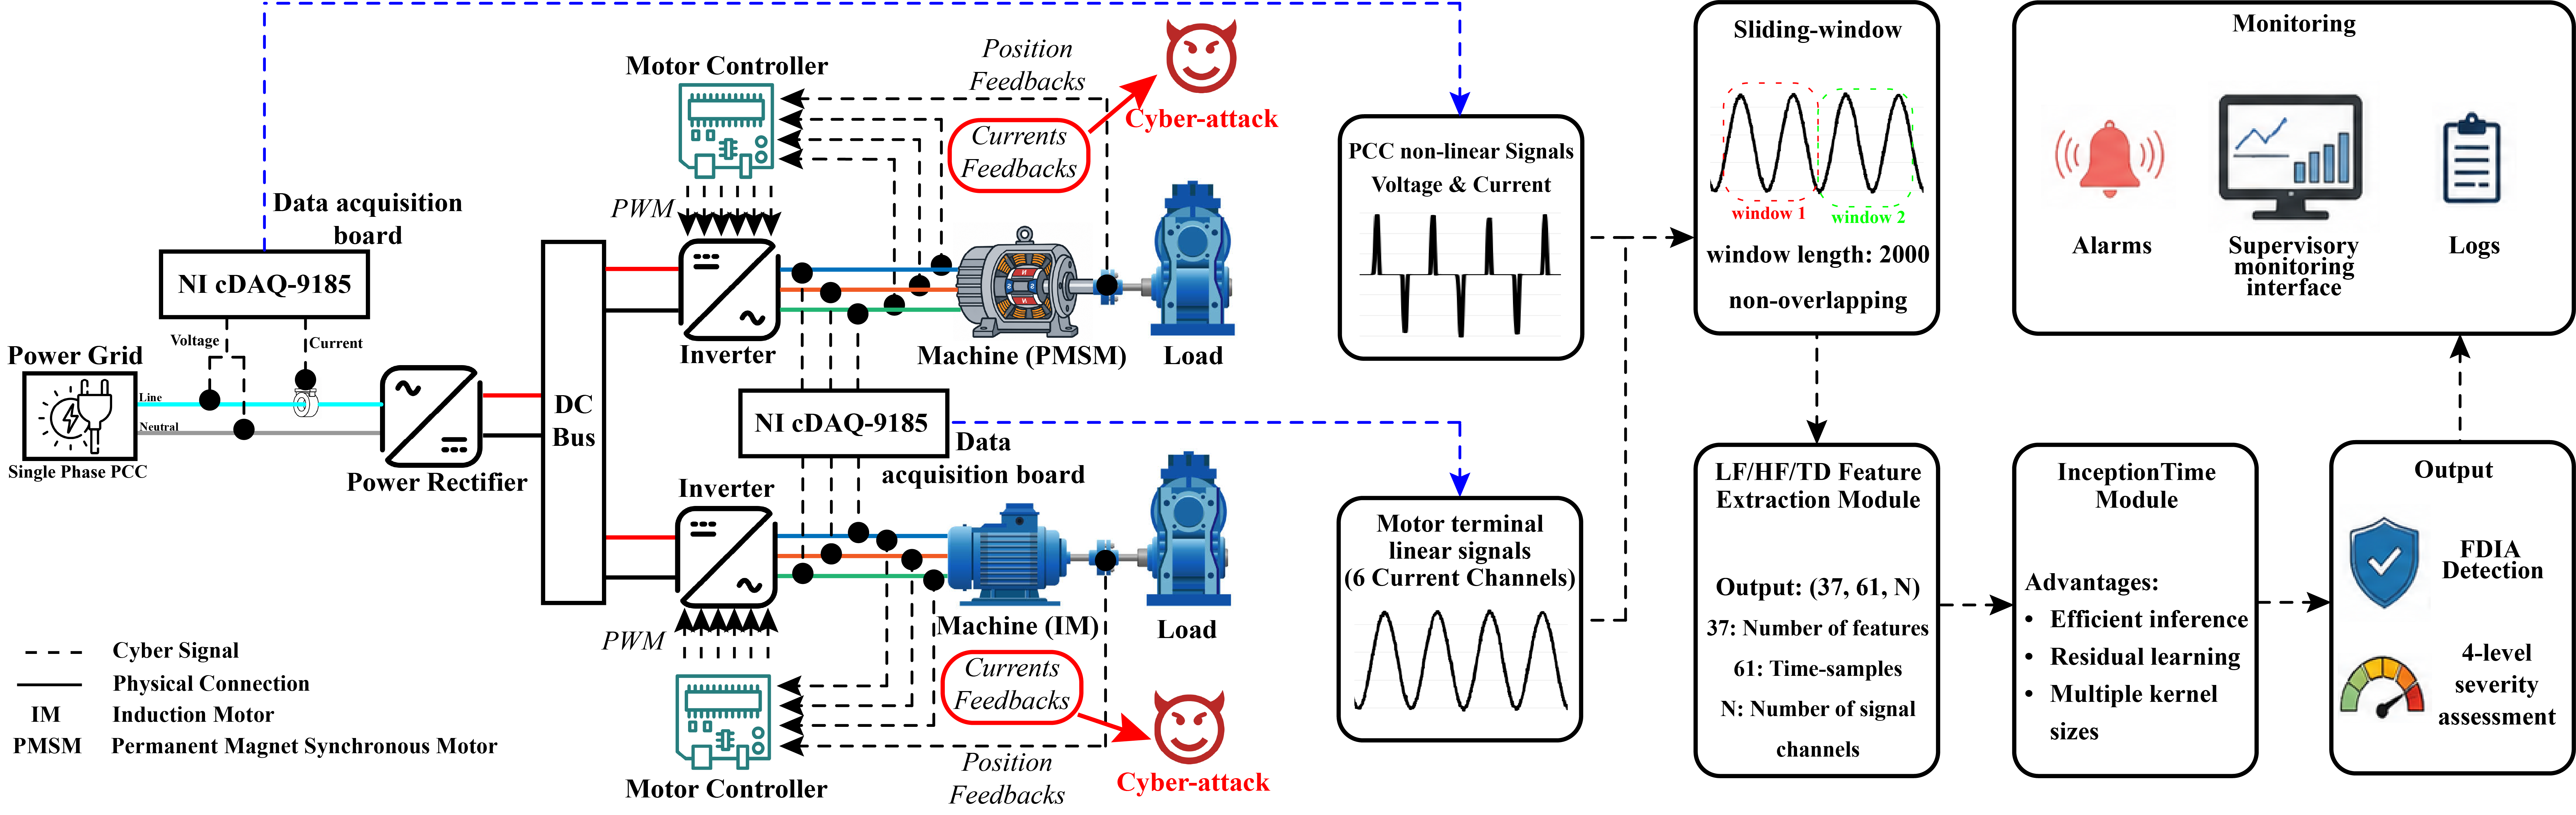
\includegraphics[width=0.95\textwidth]{figs/diagram2.png}
    \DiffOriginalCaption{Figure 1: Experimental platform used to generate current-feedback FDIAs in a heterogeneous inverter-fed motor-drive testbed.}






\end{minipage}\par\vspace{1em}
% Complete new block: fig:system_schematic
\begin{minipage}[t]{\textwidth}
\centering
\textcolor{blue}{\textbf{REVISED --- Figure 1 (main\_revised.tex)}}\par\smallskip

\centering
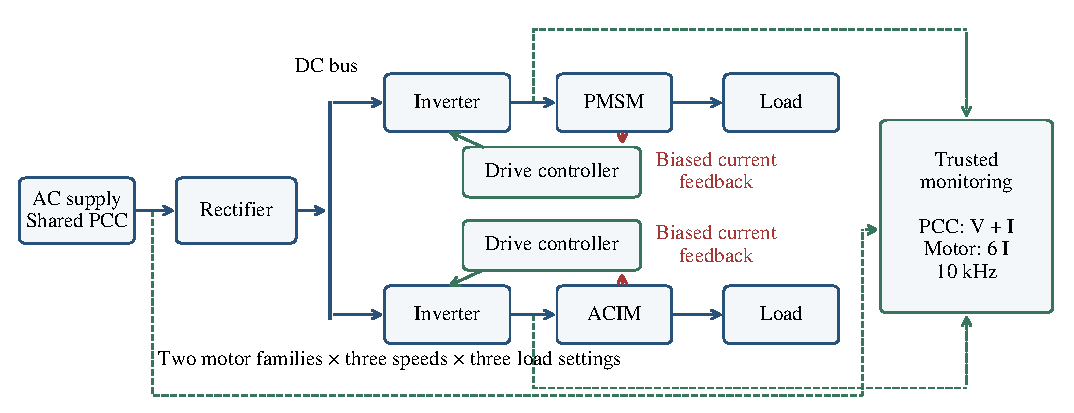
\includegraphics[width=\linewidth]{figs_revised/figure1_platform.pdf}
\caption{Experimental platform with a shared PCC, ACIM and PMSM drive branches, monitoring sensors, and current-feedback FDIA injection points.}
\label{fig:system_schematic}

\end{minipage}
\end{minipage}
\end{adjustbox}
\end{figure*}
\DIFaddend



\subsection{Attack Model, Sensing Assumptions, and Labels}
\label{sec:attack_labels}

In the testbed, the FDIA is injected into the controller's phase-current feedback path. The PCC and motor-side monitoring sensors are used as trusted measurements to record the physical response of the drive system under attack.
The monitoring sensors are isolated from the compromised controller feedback path. Thus, PCC sensing represents the nonintrusive monitoring case, while motor-side sensing serves as a performance reference. Replay, denial-of-service, monitoring-sensor attacks, and malicious command manipulation are outside the scope of this study.

Let $\mathbf{i}_{abc}(t)=[i_a(t),i_b(t),i_c(t)]^\top$ denote the true three-phase current-feedback vector \DIFaddbegin \DIFadd{in the controller's per-unit representation}\DIFaddend , and let $\tilde{\mathbf{i}}_{abc}(t)$ denote the corrupted current-feedback vector received by the motor controller. During an attack interval, the FDIA is modeled as an additive phase-current bias:
\begin{equation}
\tilde{\mathbf{i}}_{abc}(t)
=
\mathbf{i}_{abc}(t)+\boldsymbol{\alpha},
\qquad t\in[t_{\mathrm{on}},t_{\mathrm{off}}],
\label{eq:fdia_model}
\end{equation}
Here, \(\boldsymbol{\alpha}=[\alpha_a,\alpha_b,\alpha_c]^\top\) denotes the injected per-unit bias vector, with \(\boldsymbol{\alpha}=\mathbf{0}\) outside the attack interval. The tested nonzero bias magnitudes range from \(0.0005\) to \(0.0050~\mathrm{pu}\), corresponding to \(0.05\%\)--\(0.5\%\) current-feedback bias. These low-severity FDIAs are difficult to detect because their signatures can be masked by normal variation, harmonics, and PCC aggregation. \DIFaddbegin \DIFadd{The bias is normalized to the nominal controller current-feedback base. In this study, severity is defined by the injected bias magnitude; physical consequences such as shaft-torque deviation are not used as severity labels. }\DIFaddend Attack severity is measured by the largest \DIFaddbegin \DIFadd{absolute }\DIFaddend injected phase-current bias,
\(s=\|\boldsymbol{\alpha}\|_\infty\).

For binary FDIA detection, each window is labeled as
$y_{\mathrm{fdia2}}=1$ if $s>0$ and $y_{\mathrm{fdia2}}=0$ otherwise.
For \DIFaddbegin \DIFadd{joint detection and localization (}\texttt{\DIFadd{fdia3}}\DIFadd{), labels 0, 1, and 2 denote normal operation (33,054 windows), ACIM attack (13,500), and PMSM attack (13,500), respectively. Only one motor is attacked at a time.
For }\DIFaddend four-class severity assessment, the label is defined as
\DIFdelbegin \begin{displaymath}
\DIFdel{y_{\mathrm{severity4}} =
\begin{cases}
0, & s=0 \quad \text{(normal)},\\
1, & 0.0005 \leq s \leq 0.0015 \quad \text{(mild)},\\
2, & 0.0020 \leq s \leq 0.0035 \quad \text{(medium)},\\
3, & 0.0040 \leq s \leq 0.0050 \quad \text{(severe)}.
\end{cases}
}\end{displaymath}%DIFAUXCMD
\DIFdelend \DIFaddbegin \begin{equation}
\DIFadd{y_{\mathrm{severity4}} =
\begin{cases}
0, & s=0 \quad \text{(normal)},\\
1, & 0.0005 \leq s \leq 0.0015 \quad \text{(low)},\\
2, & 0.0020 \leq s \leq 0.0035 \quad \text{(medium)},\\
3, & 0.0040 \leq s \leq 0.0050 \quad \text{(high)}.
\end{cases}
\label{eq:severity_bins}
}\end{equation}\DIFaddend
\DIFdelbegin \DIFdel{corresponding to normal,mild,}\DIFdelend \DIFaddbegin \DIFadd{Cases 21--30 have $s=0.0050$ throughout because phase A remains fixed; all belong to the high-bias class. The resulting attack-window counts are 5,400 low, 7,200 }\DIFaddend medium, and \DIFdelbegin \DIFdel{severe conditions,respectively}\DIFdelend \DIFaddbegin \DIFadd{14,400 high}\DIFaddend .
Table~\ref{tab:cyberattack_dataset_structure} summarizes the swept single-phase, equal two-phase, and fixed-plus-swept two-phase FDIA cases. Across three speeds, three load settings, and two motor types, the dataset contains 540 total attack cases. Each recording \DIFdelbegin \DIFdel{consists of }\DIFdelend \DIFaddbegin \DIFadd{contains }\DIFaddend 30 consecutive 20-s episodes, with 10~s normal operation followed by 10~s FDIA operation. \DIFaddbegin \DIFadd{In total, the dataset contains 33,054 normal and 27,000 attack windows.
}



\begin{table*}[p]
\centering
\begin{adjustbox}{max width=\textwidth,max totalheight=0.87\textheight}
\begin{minipage}{\textwidth}
\centering
% Complete old block: tab:cyberattack_dataset_structure
\begin{minipage}[t]{0.48\textwidth}
\centering
\textcolor{red}{\textbf{ORIGINAL --- Table 1 (main.tex)}}\par\smallskip

\centering
\footnotesize
\DiffOriginalCaption{Table 1: FDIA dataset structure.}

\renewcommand{\arraystretch}{1.12}
\begin{adjustbox}{max width=\linewidth}\begin{tabular}{c c c c}
\hline
Cases & Phases & Bias Pattern & Total \\
\hline
1--10  & A   & $\alpha_a$: $0.0005$--$0.0050$ & 180 \\
11--20 & A,B & $\alpha_a=\alpha_b$: $0.0005$--$0.0050$ & 180 \\
21--30 & A,B & $\alpha_a=0.0050$, $\alpha_b$: $0.0005$--$0.0050$ & 180 \\
\hline
\multicolumn{3}{r}{Overall} & 540 \\
\hline
\end{tabular}\end{adjustbox}
\vspace{1mm}
\begin{flushleft}
\footnotesize Each case group is evaluated over 3 speeds, 3 load settings, and 2 motor types. For all cases, unspecified phase biases are zero.
\end{flushleft}

\end{minipage}\hfill%
% Complete new block: tab:cyberattack_dataset_structure
\begin{minipage}[t]{0.48\textwidth}
\centering
\textcolor{blue}{\textbf{REVISED --- Table 1 (main\_revised.tex)}}\par\smallskip

\centering
\footnotesize
\caption{FDIA dataset structure.}
\label{tab:cyberattack_dataset_structure}
\renewcommand{\arraystretch}{1.12}
\begin{tabular}{c c c c}
\hline
Cases & Phases & Bias Pattern & Total \\
\hline
1--10  & A   & $\alpha_a$: $0.0005$--$0.0050$ & 180 \\
11--20 & A,B & $\alpha_a=\alpha_b$: $0.0005$--$0.0050$ & 180 \\
21--30 & A,B & $\alpha_a=0.0050$, $\alpha_b$: $0.0005$--$0.0050$ & 180 \\
\hline
\multicolumn{3}{r}{Overall} & 540 \\
\hline
\end{tabular}
\vspace{1mm}
\begin{flushleft}
\footnotesize Each case group is evaluated over 3 speeds, 3 load settings, and 2 motor types. For all cases, unspecified phase biases are zero.
\end{flushleft}

\end{minipage}
\end{minipage}
\end{adjustbox}
\end{table*}
\DIFaddend




\subsection{Data Acquisition and Operating Conditions}
\label{sec:data_acquisition}

Electrical measurements were acquired from the testbed using a National Instruments cDAQ-9185 chassis and a custom data-collector interface board. The interface board routed synchronized motor-side and PCC-side analog channels to the acquisition system. \DIFaddbegin \DIFadd{Table~\ref{tab:measurement_streams} summarizes the measured signals and channel counts. }\DIFaddend Three brake-excitation settings were tested for each machine: 1--3~V for the ACIM branch and 2--4~V for the PMSM branch. Because torque was not directly measured, these brake-excitation voltages are used as load-condition labels. All channels were sampled at 10~kHz and stored in TDMS format. For learning-based analysis, each record was segmented into non-overlapping 0.2~s windows containing 2{,}000 samples. \DIFdelbegin \DIFdel{This non-overlapping segmentation prevents temporal leakagebefore train/validation/test splitting}\DIFdelend \DIFaddbegin \DIFadd{To prevent temporal leakage, complete recordings and all their episodes were assigned to separate training, validation, and test sets. Normalization statistics were fitted using training recordings only}\DIFaddend . The resulting dataset dimensions, input configurations, severity-label distributions, and evaluation protocols are summarized in Table~\ref{tab:evaluation_protocols}. \DIFaddbegin \DIFadd{Three seeds (1234, 2234, and 3234) changed the recording assignment and model initialization; recordings can recur across repeats.
}



\begin{figure*}[p]
\centering
\begin{adjustbox}{max width=\textwidth,max totalheight=0.87\textheight}
\begin{minipage}{\textwidth}
\centering
% Complete old block: fig:lfhf_motor_pcc_examples
\begin{minipage}[t]{\textwidth}
\centering
\textcolor{red}{\textbf{ORIGINAL --- Figure 2 (main.tex)}}\par\smallskip

    \centering
    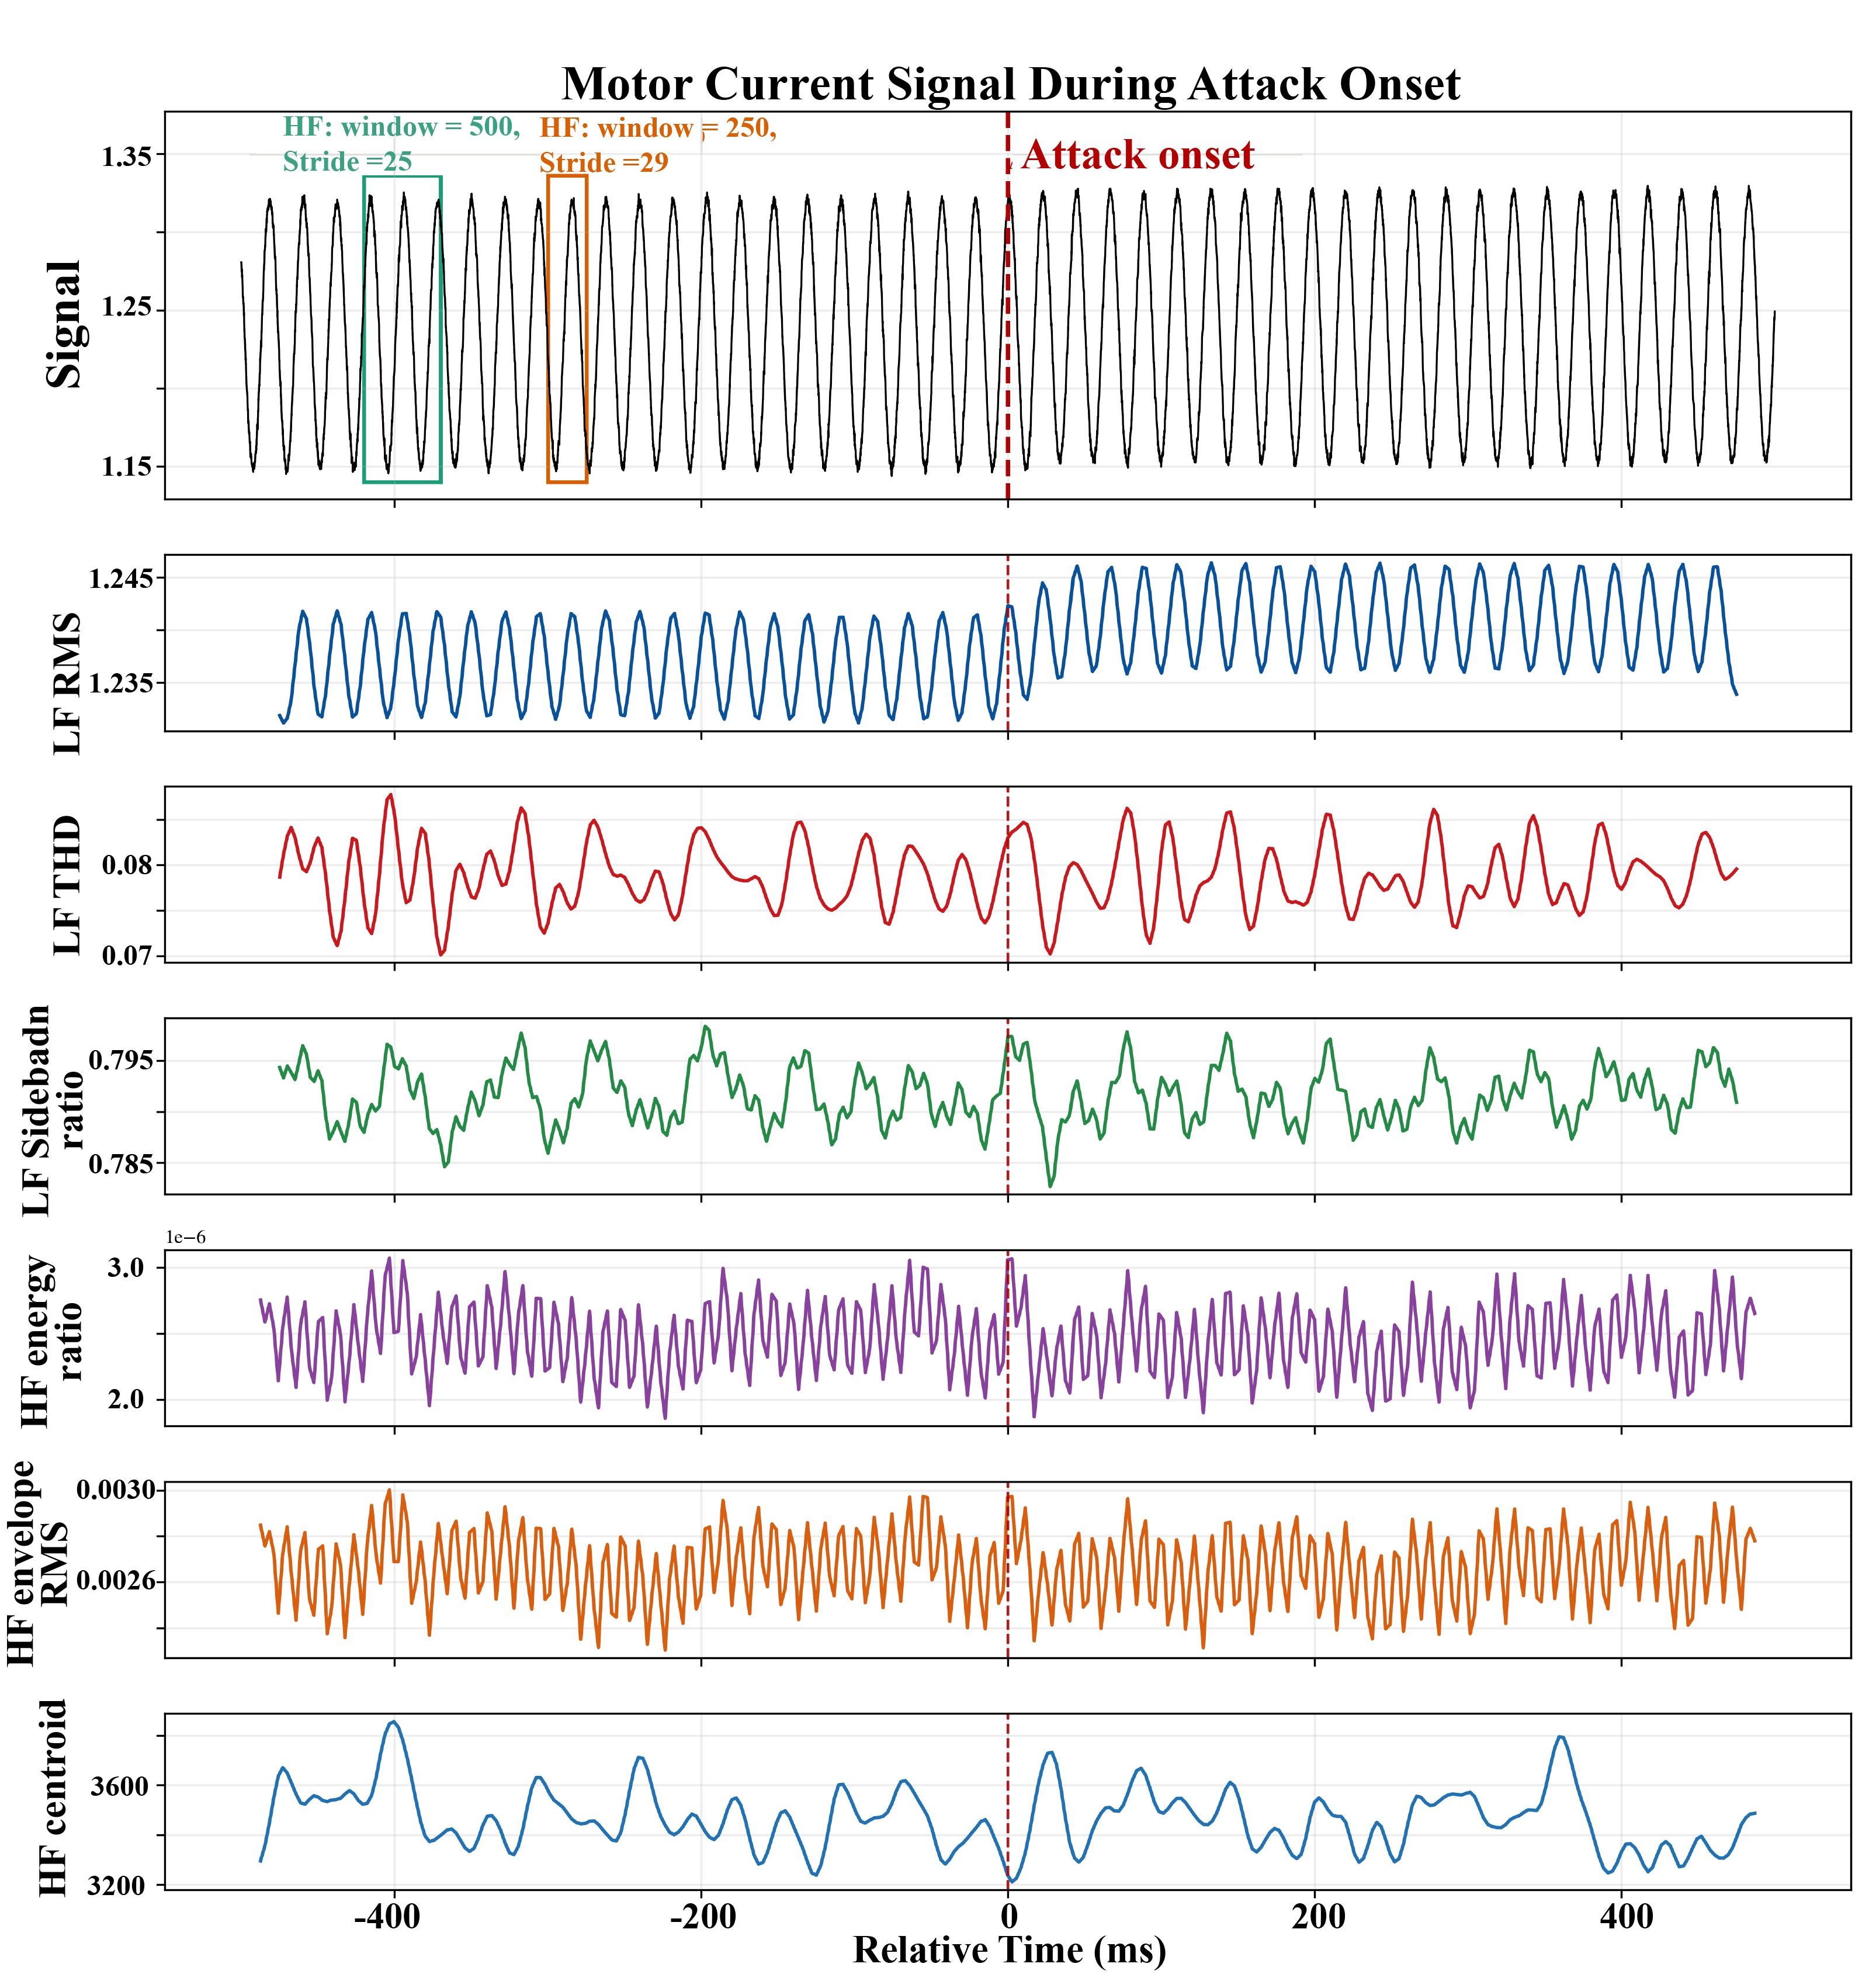
\includegraphics[width=0.49\textwidth]{figs/tdms_lfhf_window_example_acim_179p9s_separate_revised.png}
    \hfill
    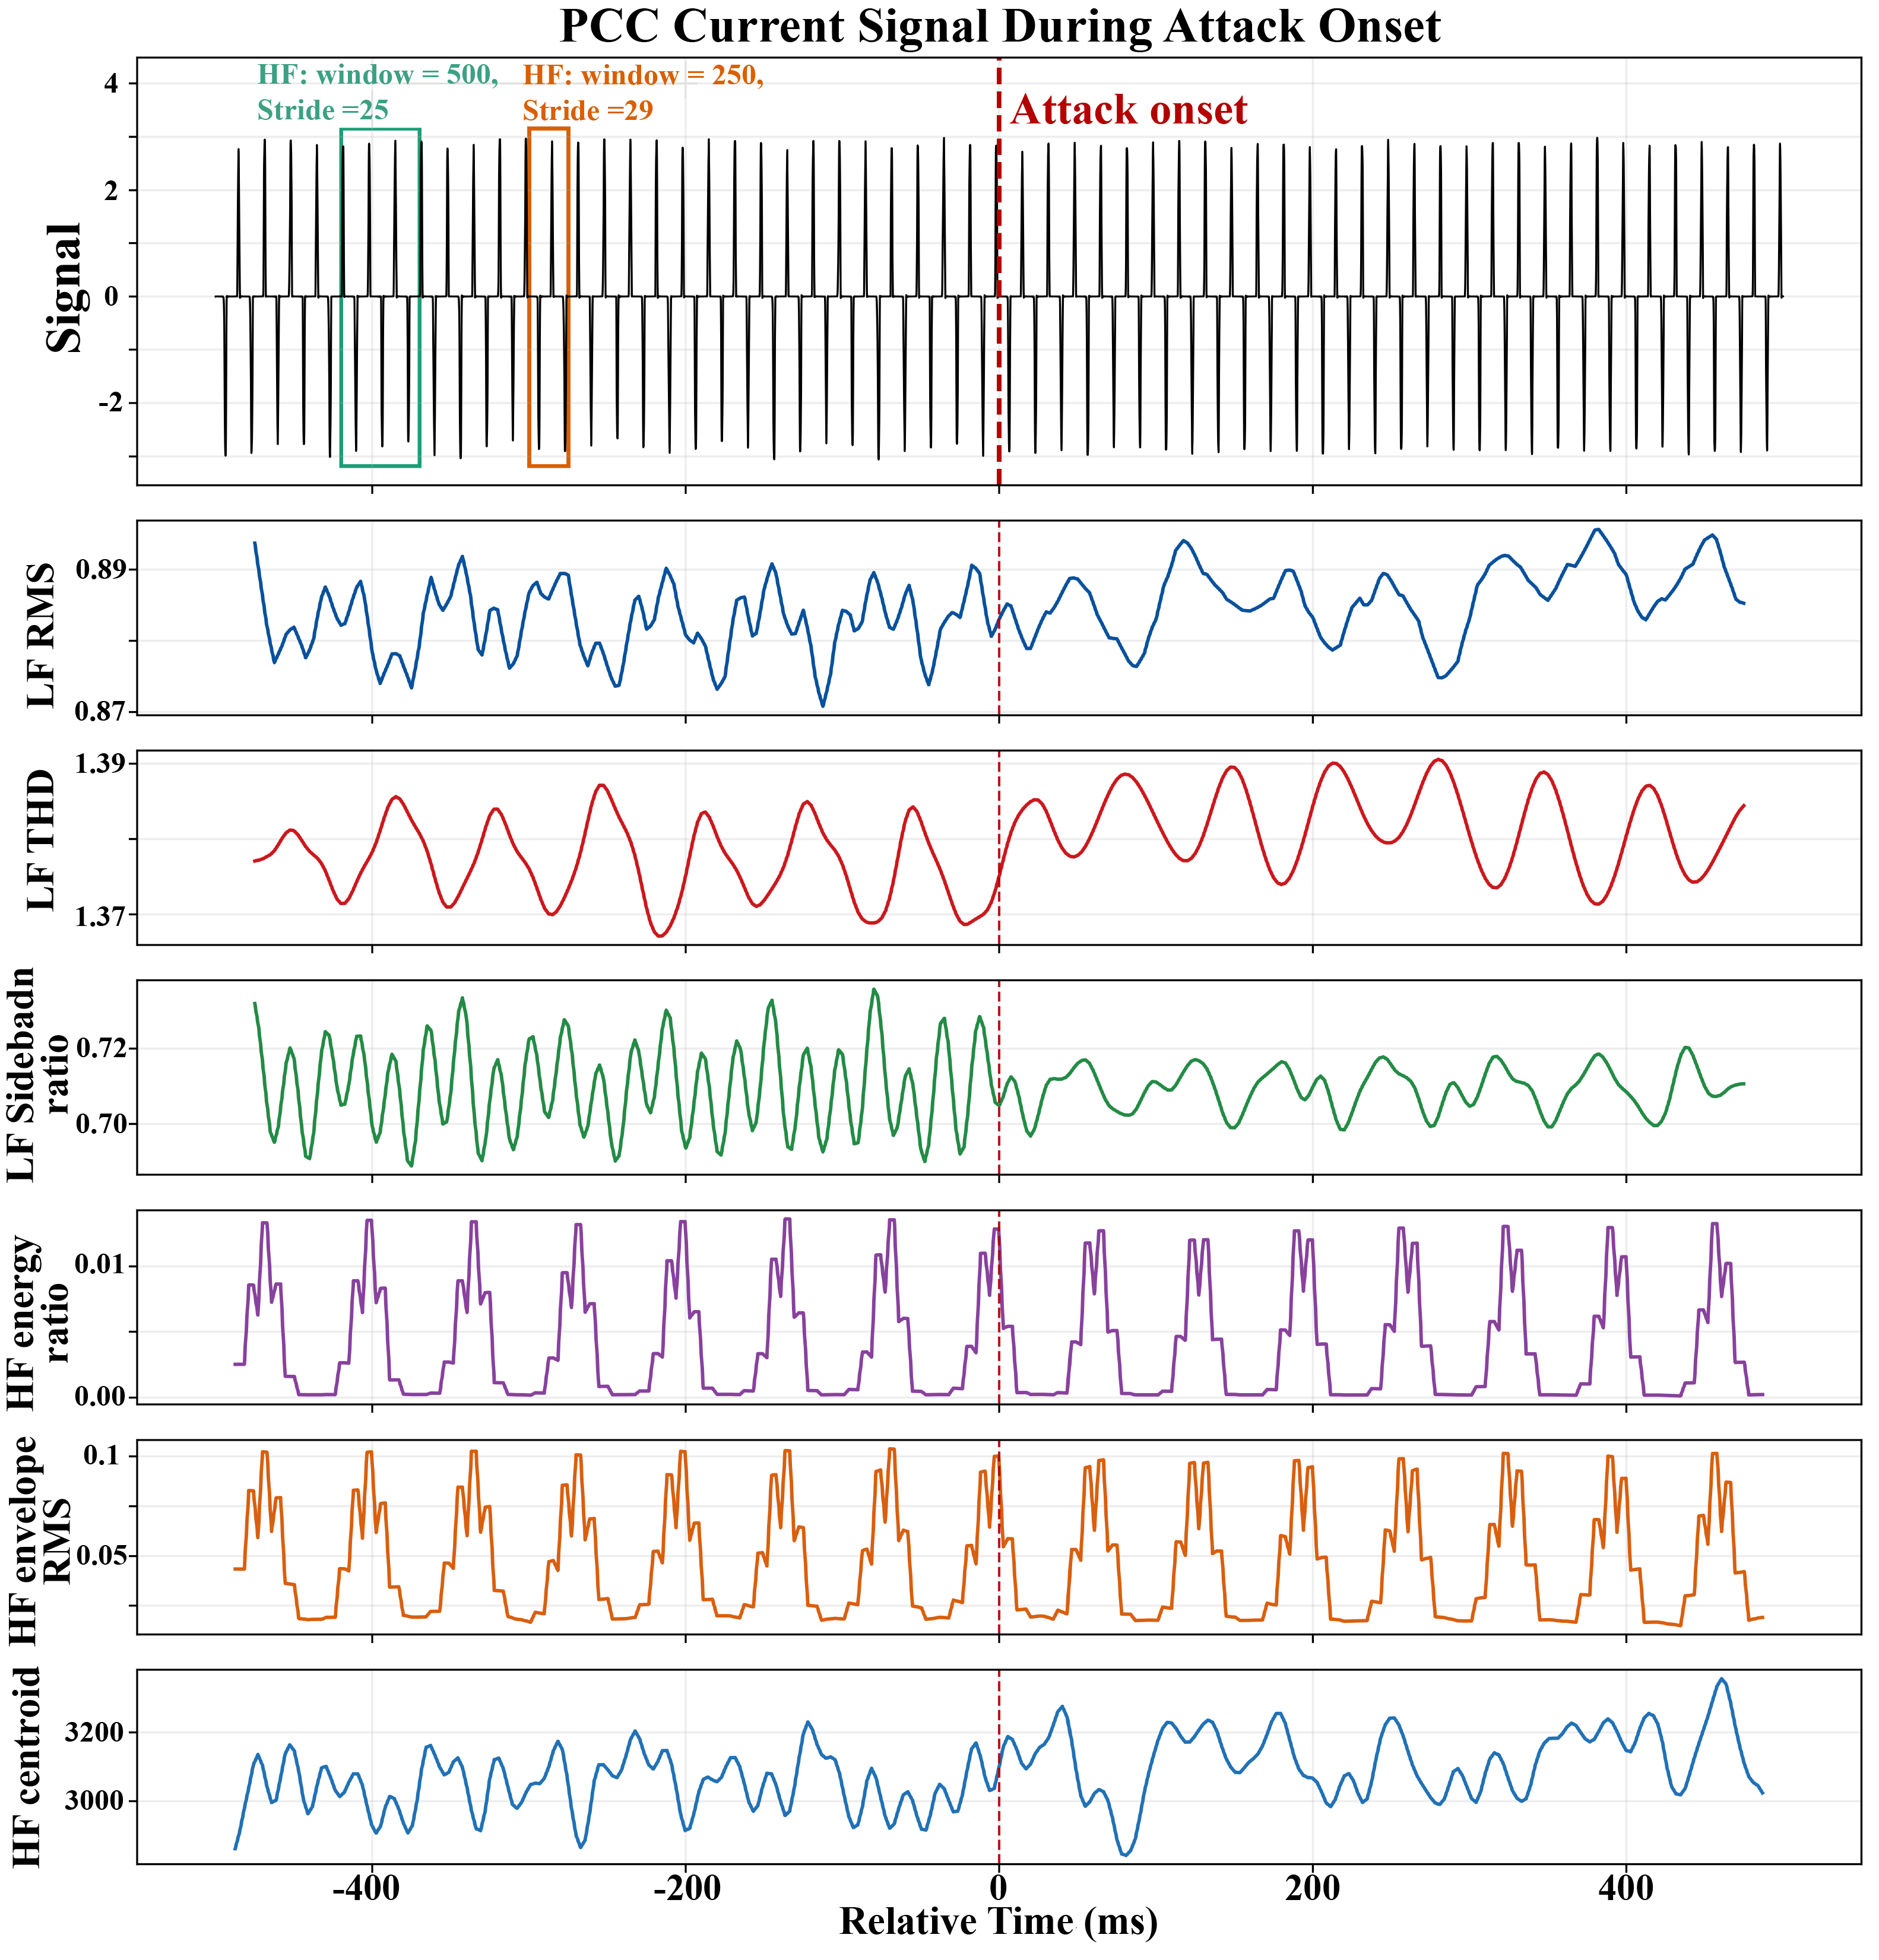
\includegraphics[width=0.49\textwidth]{figs/tdms_lfhf_window_example_pcc_179p9s_separate_revised.png}
    \DiffOriginalCaption{Figure 2: Representative motor-side and PCC-side signals at attack onset with the corresponding LF/HF feature responses.}


\end{minipage}\par\vspace{1em}
% Complete new block: fig:lfhf_motor_pcc_examples
\begin{minipage}[t]{\textwidth}
\centering
\textcolor{blue}{\textbf{REVISED --- Figure 2 (main\_revised.tex)}}\par\smallskip

\centering
\begingroup\setlength{\unitlength}{1bp}
\resizebox{\linewidth}{!}{\begin{picture}(515.52,292)
\put(126.00000,286.00000){\makebox(0,0){\color{black}\fontsize{9bp}{10bp}\selectfont Motor current}}
\put(112.00000,274.00000){\makebox(0,0){\color{green!45!black}\fontsize{8bp}{9bp}\selectfont LF: 500/25}}
\put(192.00000,274.00000){\makebox(0,0){\color{orange!85!black}\fontsize{8bp}{9bp}\selectfont HF: 250/29}}
\put(62.00000,211){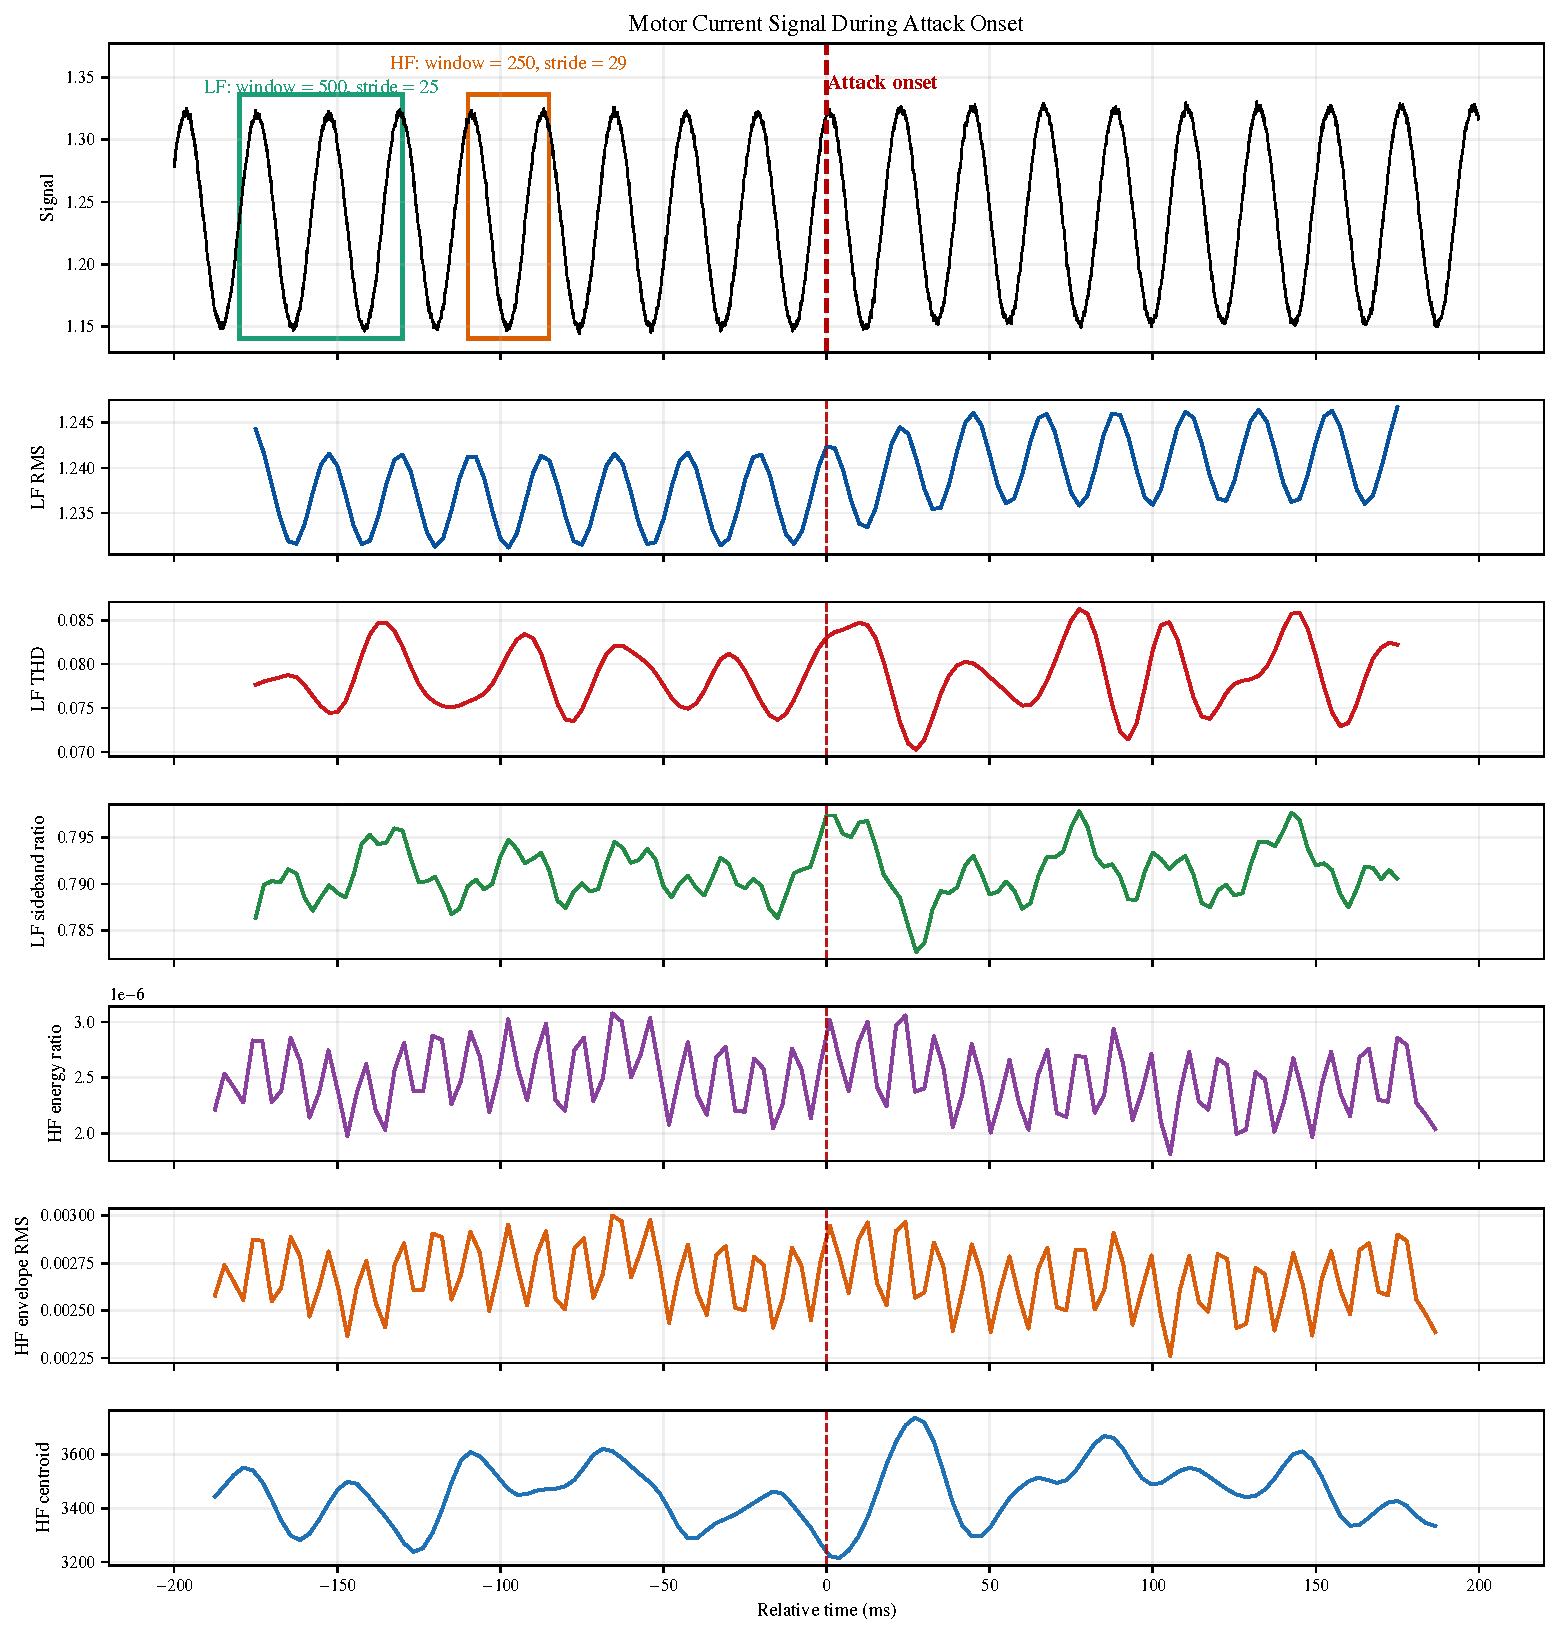
\includegraphics[viewport=52.29375000 615.56156250 741.04375000 764.00312500,clip,width=186bp,height=50bp]{figs_revised/original_sources/tdms_lfhf_window_example_acim_179p9s_separate.pdf}}
\put(62.00000,211){\color{black}\linethickness{0.3bp}\framebox(186,50){}}
\put(15.00000,236.00000){\makebox(0,0){\color{black}\fontsize{7.5bp}{8.5bp}\selectfont \shortstack{Signal}}}
\put(59.00000,215.22545){\makebox(0,0)[r]{\color{black}\fontsize{7.5bp}{8.5bp}\selectfont 1.15}}
\put(59.00000,235.35151){\makebox(0,0)[r]{\color{black}\fontsize{7.5bp}{8.5bp}\selectfont 1.25}}
\put(59.00000,255.47756){\makebox(0,0)[r]{\color{black}\fontsize{7.5bp}{8.5bp}\selectfont 1.35}}
\put(62.00000,179){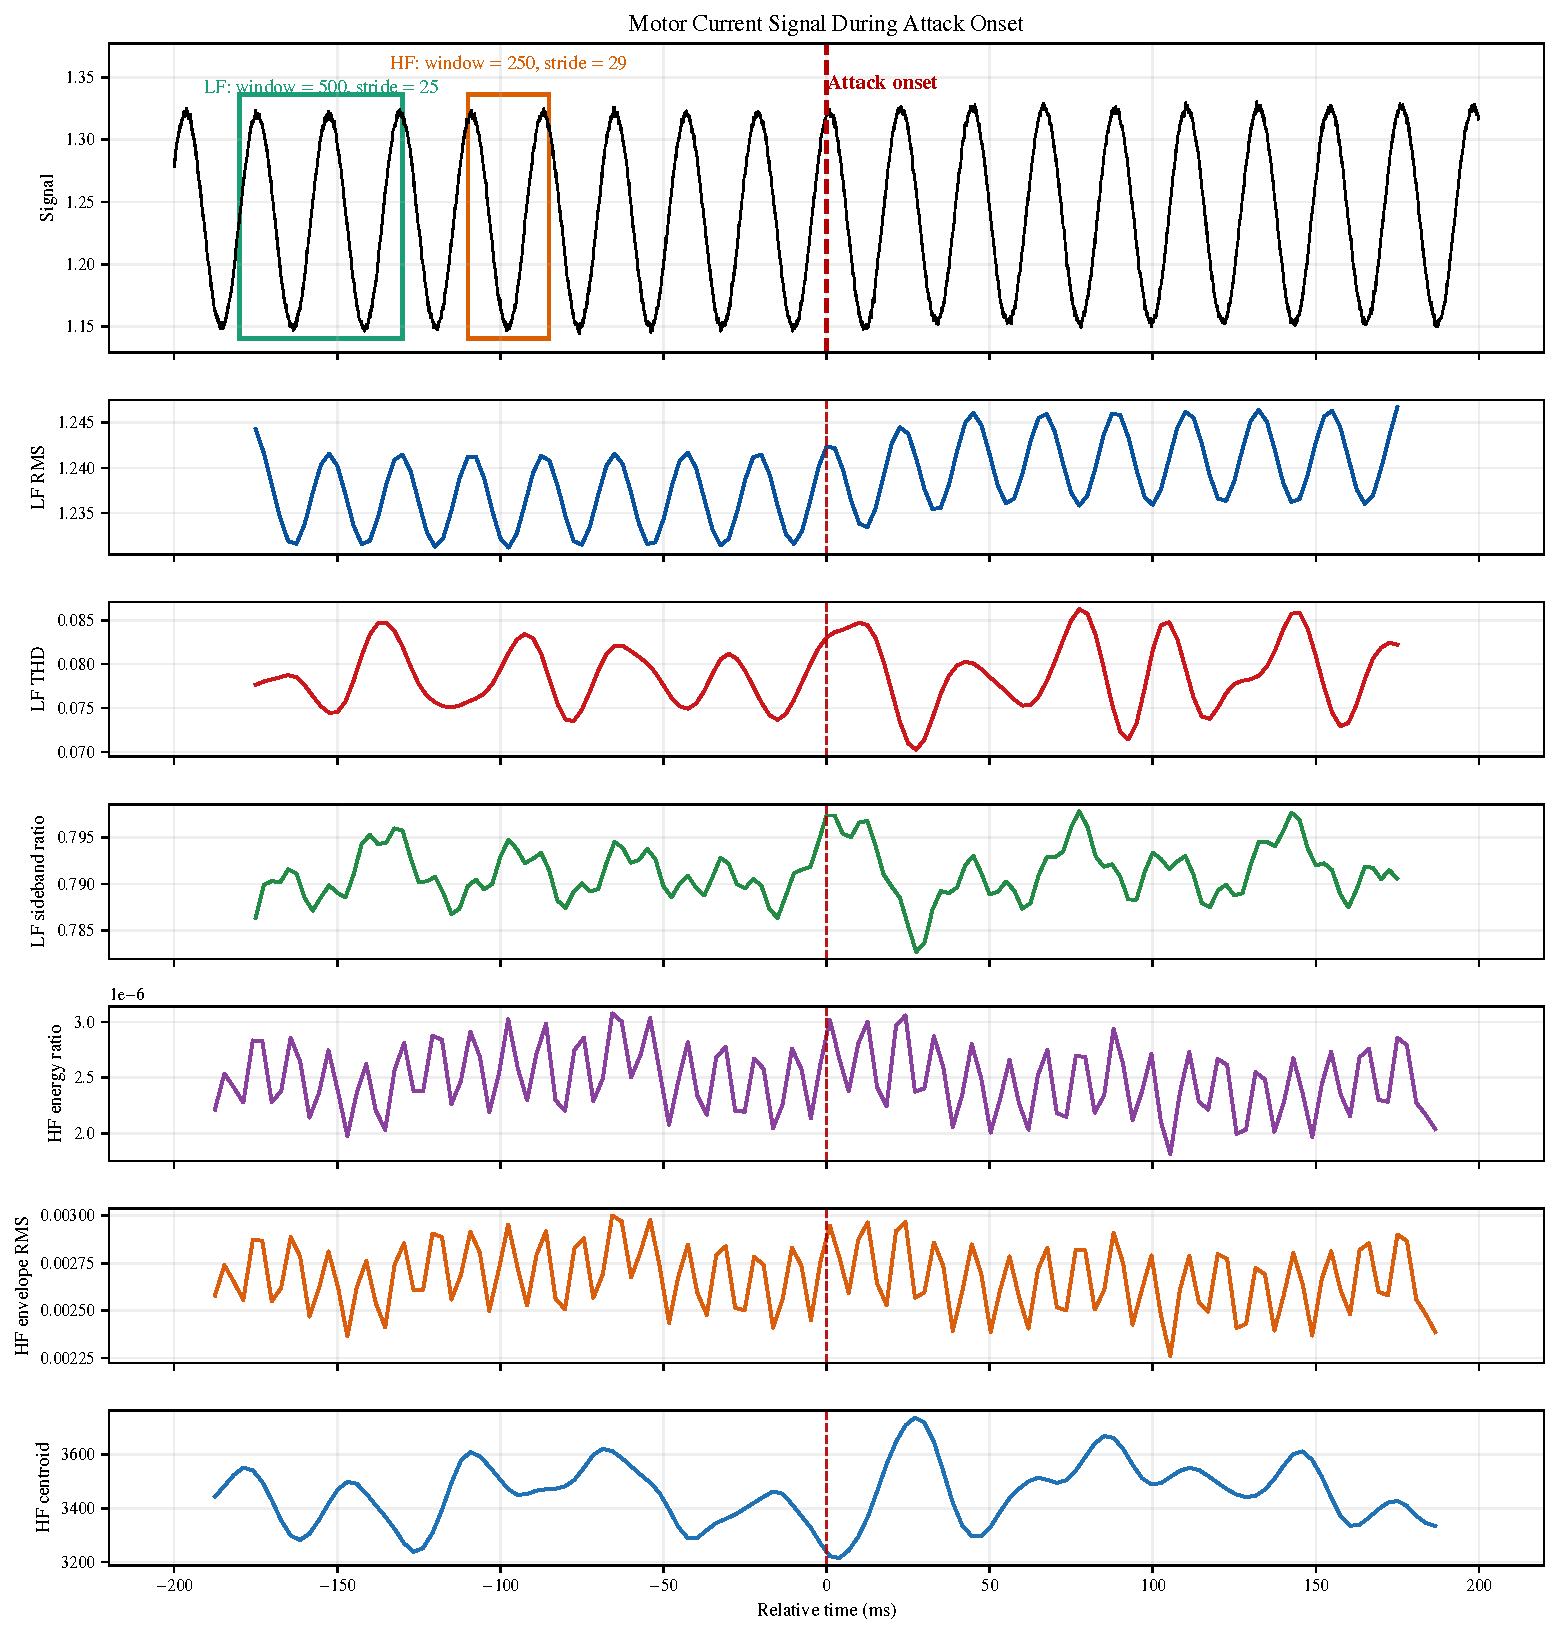
\includegraphics[viewport=52.29375000 518.55078125 741.04375000 592.77156250,clip,width=186bp,height=24bp]{figs_revised/original_sources/tdms_lfhf_window_example_acim_179p9s_separate.pdf}}
\put(62.00000,179){\color{black}\linethickness{0.3bp}\framebox(186,24){}}
\put(15.00000,191.00000){\makebox(0,0){\color{black}\fontsize{7.5bp}{8.5bp}\selectfont \shortstack{LF\\RMS}}}
\put(59.00000,185.47648){\makebox(0,0)[r]{\color{black}\fontsize{7.5bp}{8.5bp}\selectfont 1.235}}
\put(59.00000,199.47430){\makebox(0,0)[r]{\color{black}\fontsize{7.5bp}{8.5bp}\selectfont 1.245}}
\put(62.00000,147){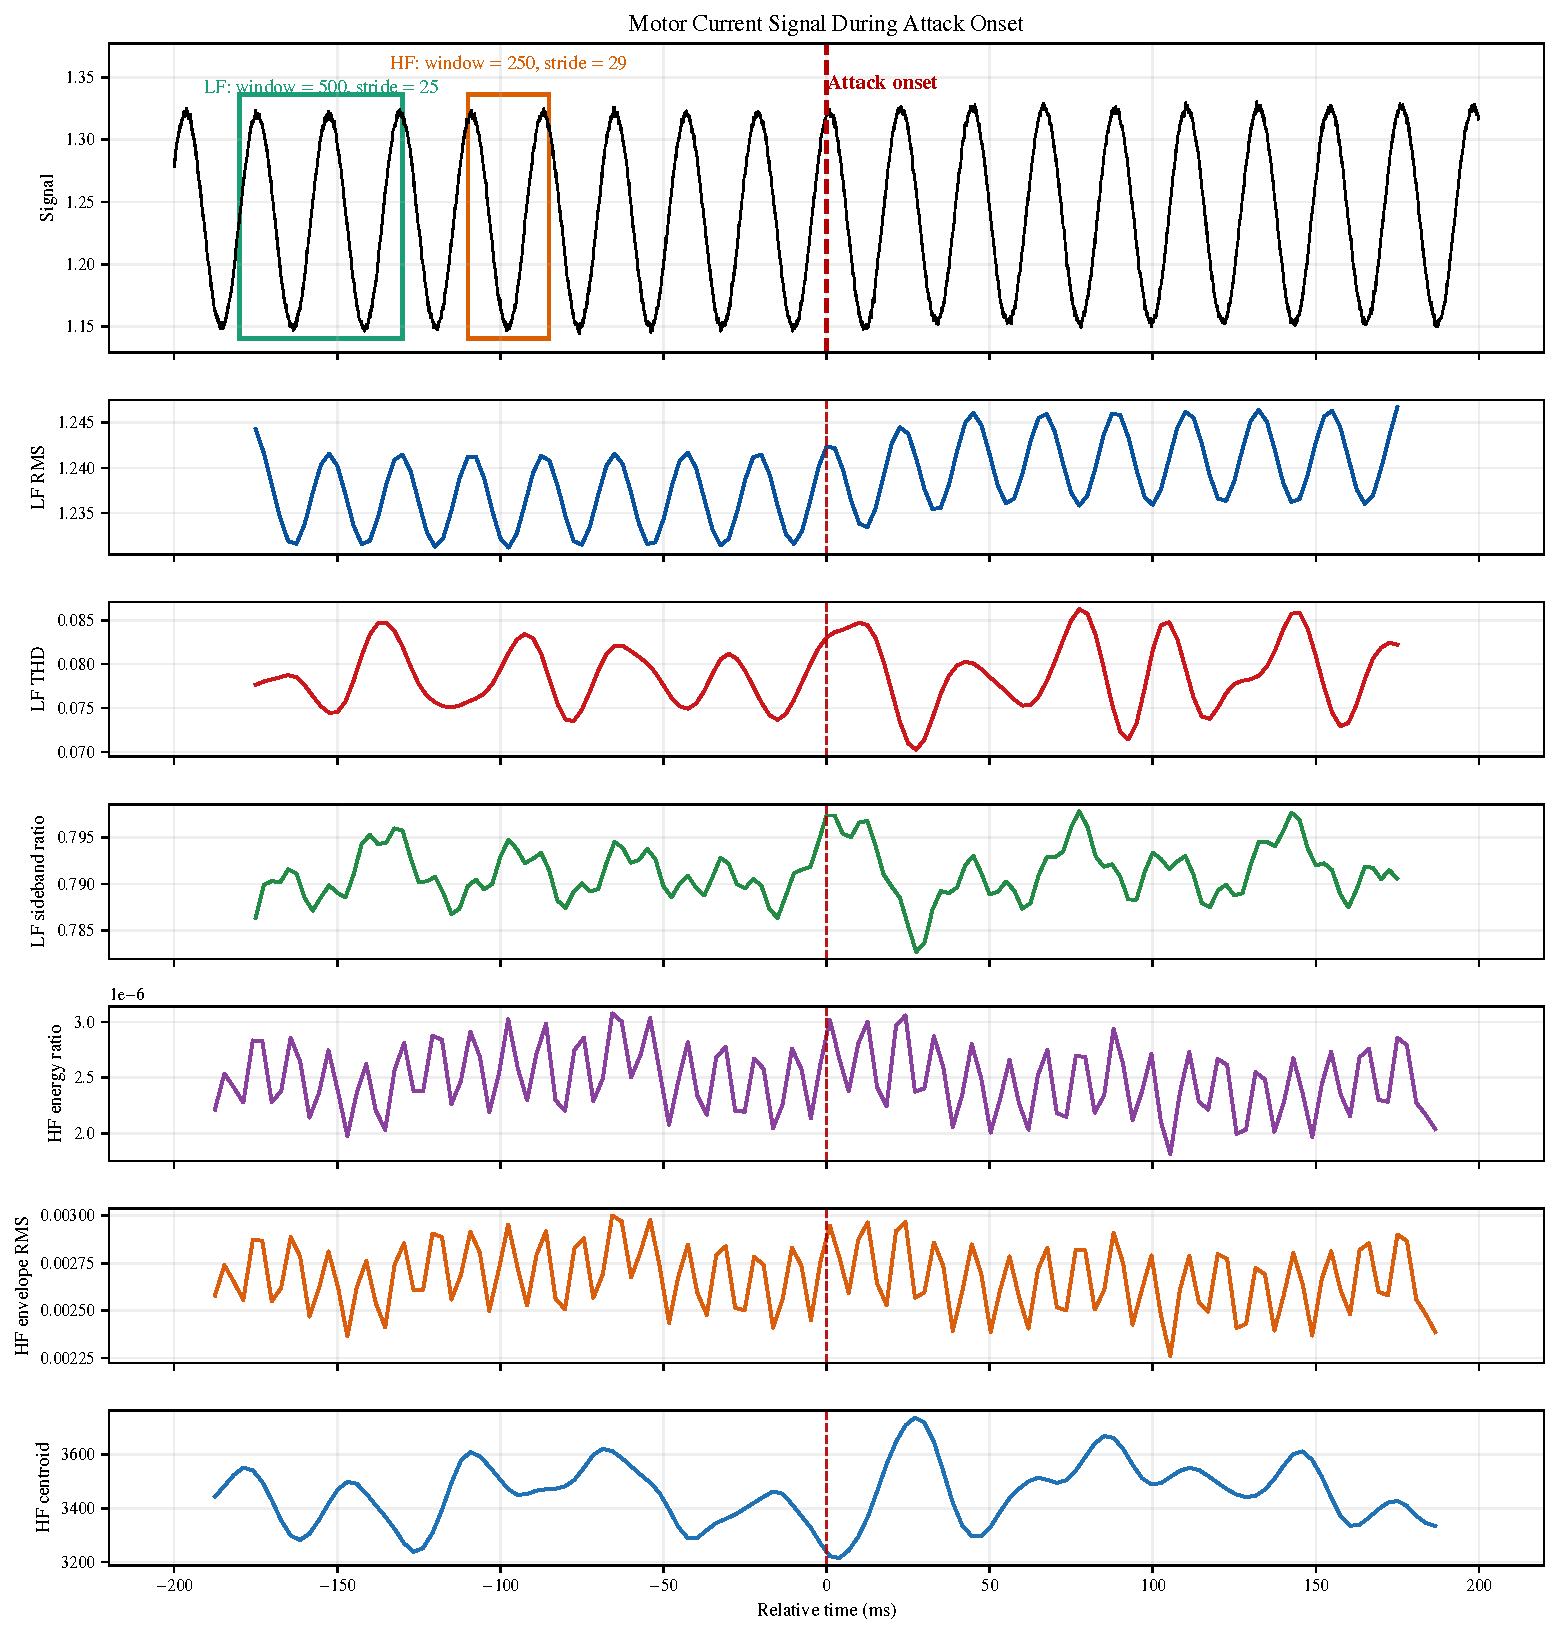
\includegraphics[viewport=52.29375000 421.54000000 741.04375000 495.76078125,clip,width=186bp,height=24bp]{figs_revised/original_sources/tdms_lfhf_window_example_acim_179p9s_separate.pdf}}
\put(62.00000,147){\color{black}\linethickness{0.3bp}\framebox(186,24){}}
\put(15.00000,159.00000){\makebox(0,0){\color{black}\fontsize{7.5bp}{8.5bp}\selectfont \shortstack{LF\\THD}}}
\put(59.00000,147.76613){\makebox(0,0)[r]{\color{black}\fontsize{7.5bp}{8.5bp}\selectfont 0.070}}
\put(59.00000,168.19185){\makebox(0,0)[r]{\color{black}\fontsize{7.5bp}{8.5bp}\selectfont 0.085}}
\put(62.00000,115){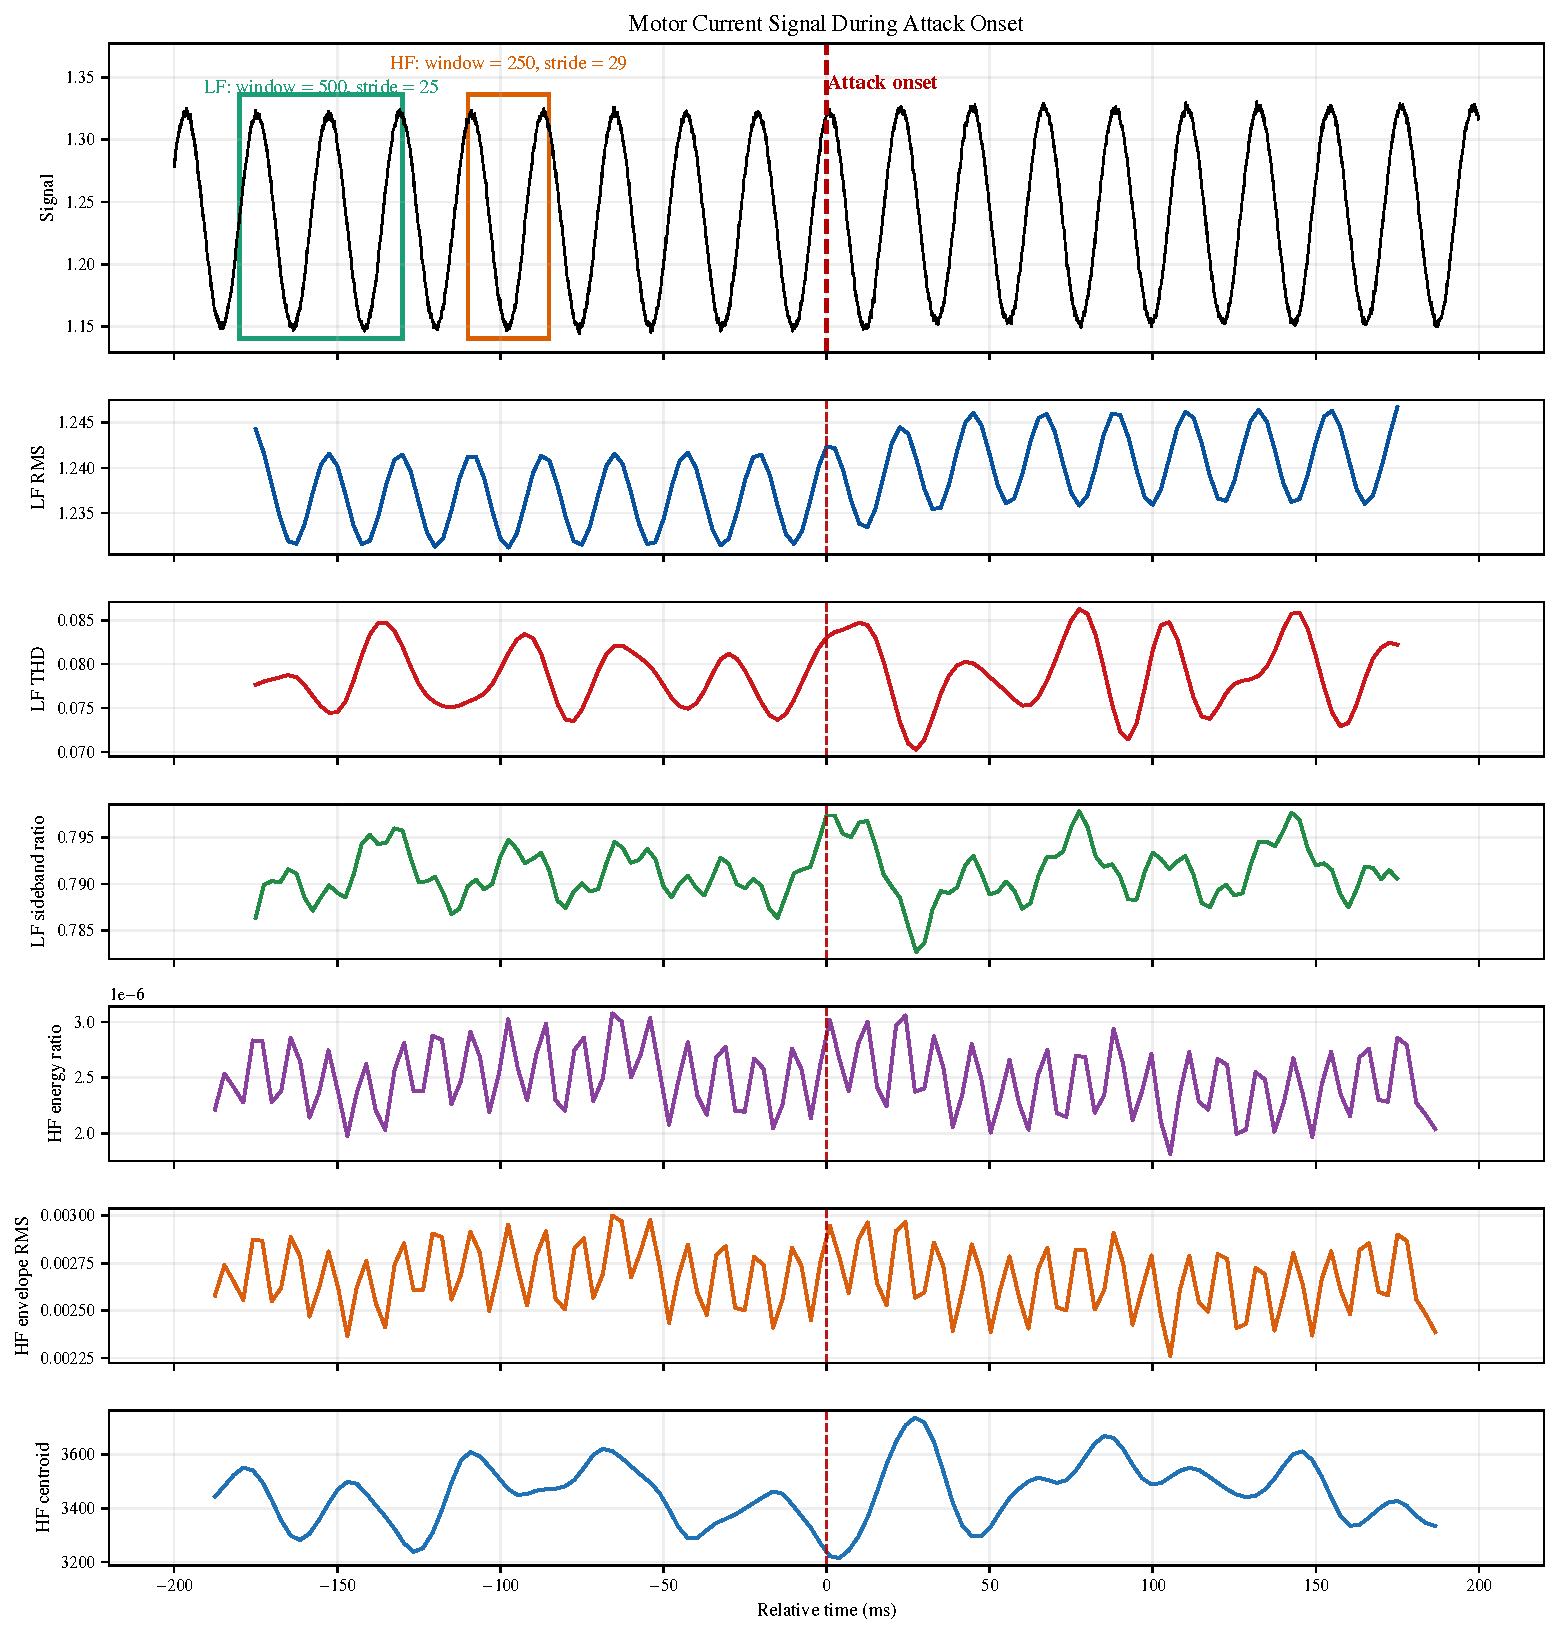
\includegraphics[viewport=52.29375000 324.52921875 741.04375000 398.75000000,clip,width=186bp,height=24bp]{figs_revised/original_sources/tdms_lfhf_window_example_acim_179p9s_separate.pdf}}
\put(62.00000,115){\color{black}\linethickness{0.3bp}\framebox(186,24){}}
\put(15.00000,127.00000){\makebox(0,0){\color{black}\fontsize{7.5bp}{8.5bp}\selectfont \shortstack{LF\\sideband\\ratio}}}
\put(59.00000,119.40473){\makebox(0,0)[r]{\color{black}\fontsize{7.5bp}{8.5bp}\selectfont 0.785}}
\put(59.00000,133.80825){\makebox(0,0)[r]{\color{black}\fontsize{7.5bp}{8.5bp}\selectfont 0.795}}
\put(62.00000,83){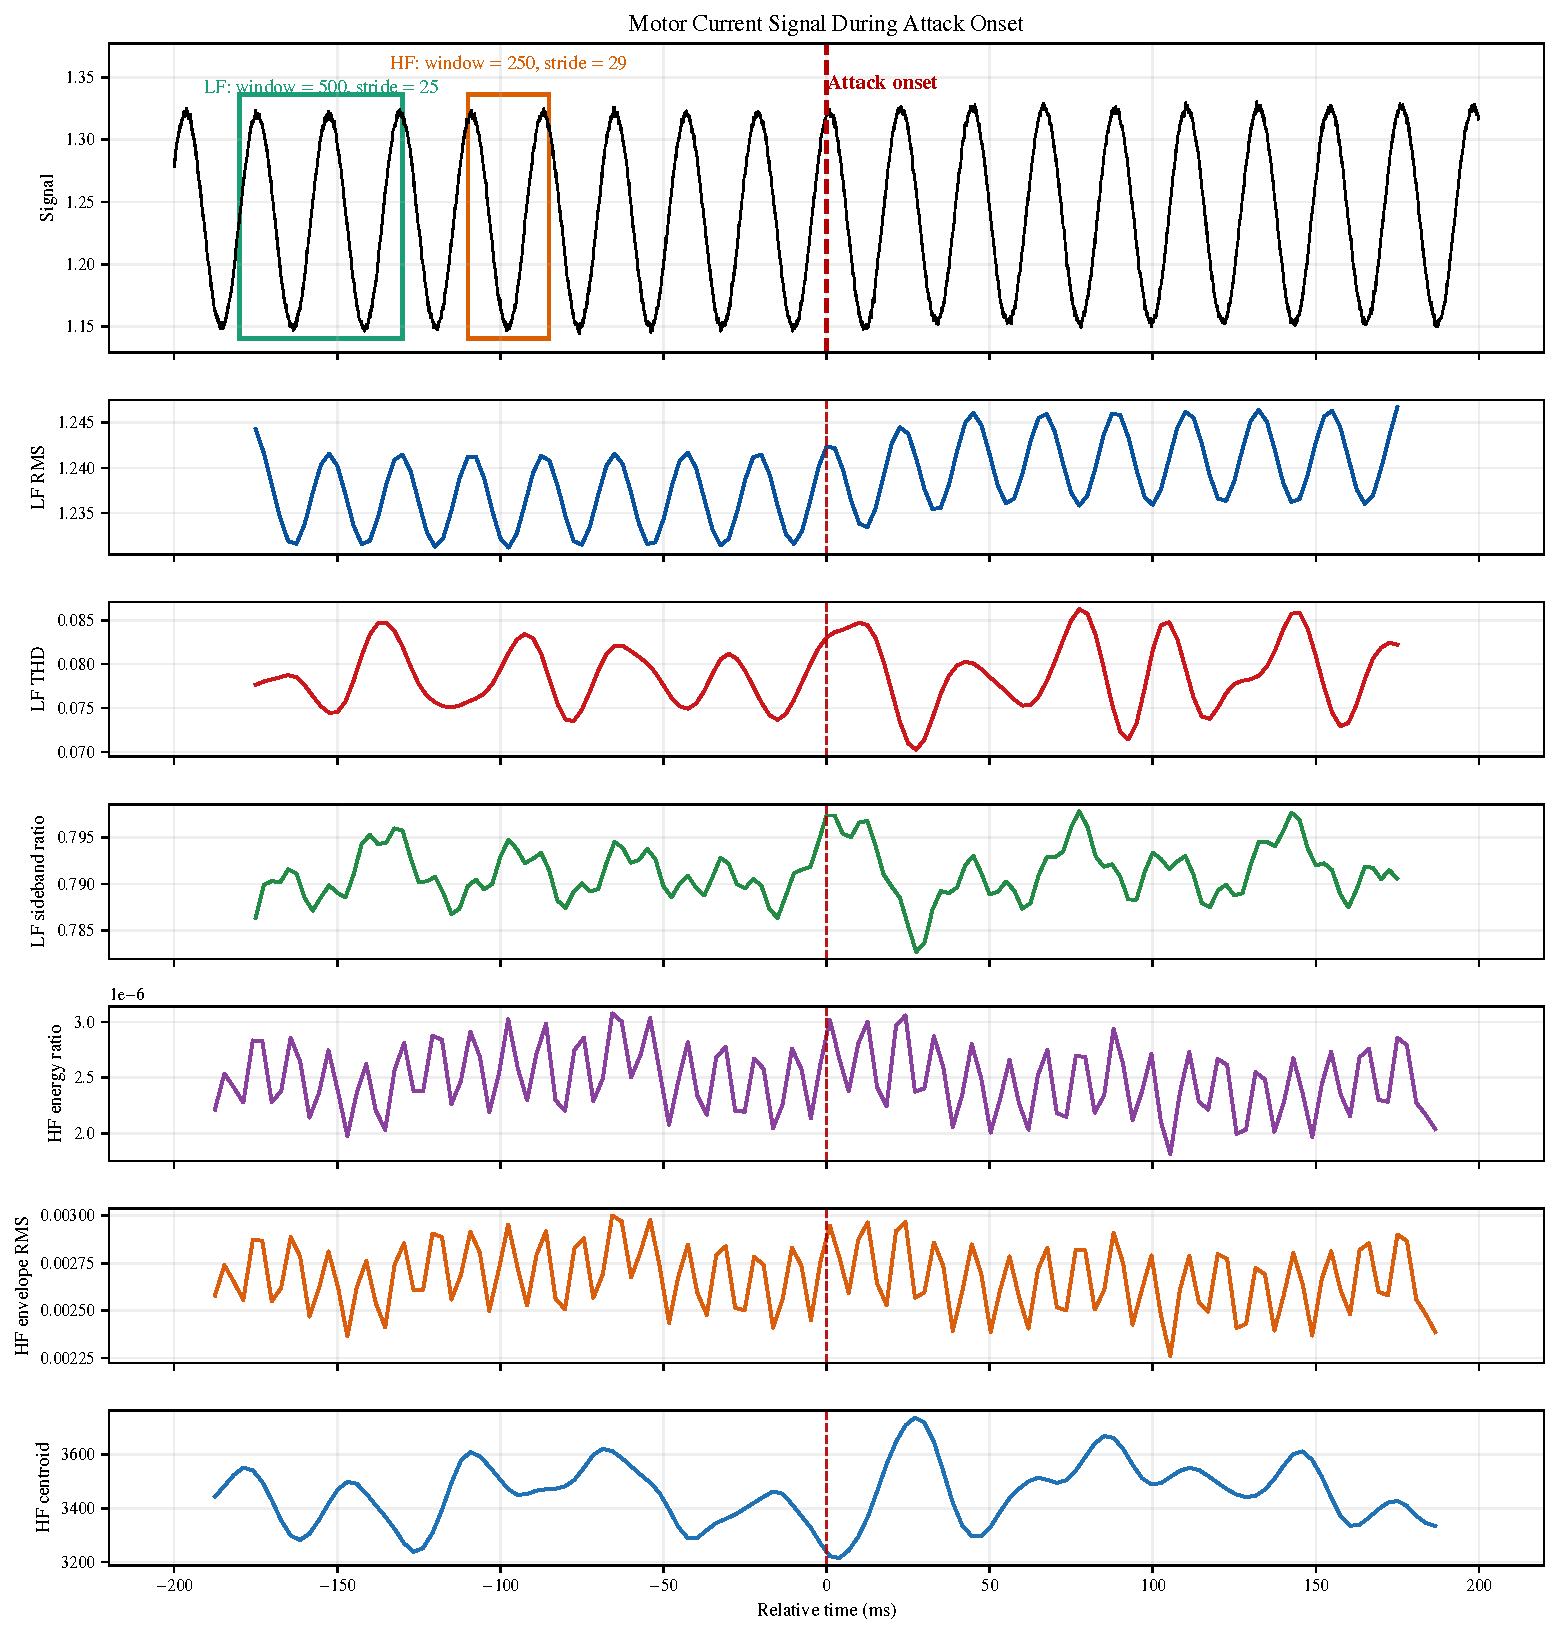
\includegraphics[viewport=52.29375000 227.51843750 741.04375000 301.73921875,clip,width=186bp,height=24bp]{figs_revised/original_sources/tdms_lfhf_window_example_acim_179p9s_separate.pdf}}
\put(62.00000,83){\color{black}\linethickness{0.3bp}\framebox(186,24){}}
\put(15.00000,95.00000){\makebox(0,0){\color{black}\fontsize{7.5bp}{8.5bp}\selectfont \shortstack{HF energy\\ratio}}}
\put(59.00000,87.26000){\makebox(0,0)[r]{\color{black}\fontsize{7.5bp}{8.5bp}\selectfont 2.0e-6}}
\put(59.00000,104.58237){\makebox(0,0)[r]{\color{black}\fontsize{7.5bp}{8.5bp}\selectfont 3.0e-6}}
\put(62.00000,51){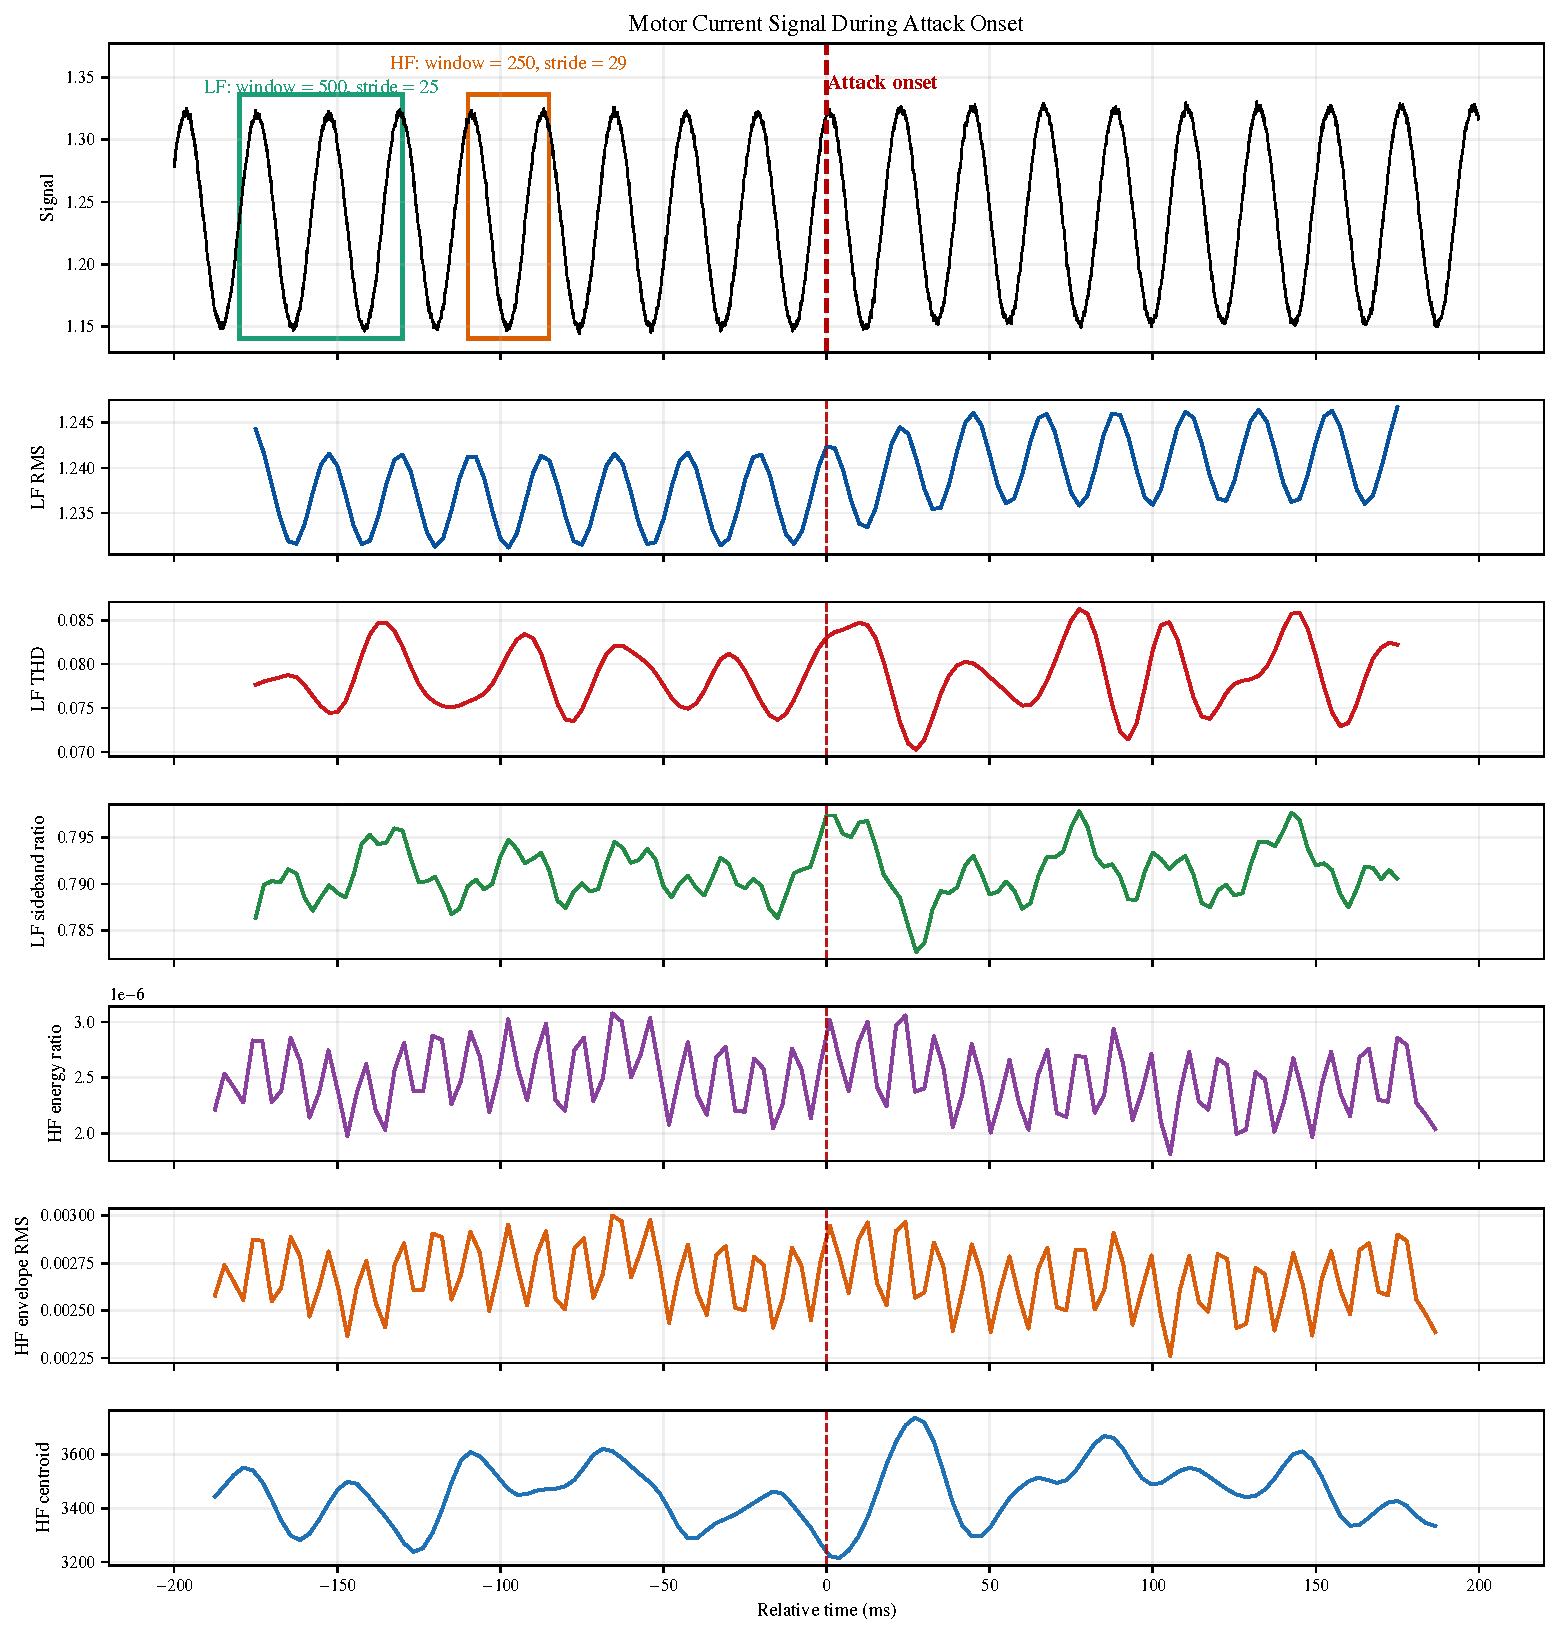
\includegraphics[viewport=52.29375000 130.50765625 741.04375000 204.72843750,clip,width=186bp,height=24bp]{figs_revised/original_sources/tdms_lfhf_window_example_acim_179p9s_separate.pdf}}
\put(62.00000,51){\color{black}\linethickness{0.3bp}\framebox(186,24){}}
\put(15.00000,63.00000){\makebox(0,0){\color{black}\fontsize{7.5bp}{8.5bp}\selectfont \shortstack{HF\\envelope\\RMS}}}
\put(59.00000,51.77401){\makebox(0,0)[r]{\color{black}\fontsize{7.5bp}{8.5bp}\selectfont 0.00225}}
\put(59.00000,73.87061){\makebox(0,0)[r]{\color{black}\fontsize{7.5bp}{8.5bp}\selectfont 0.00300}}
\put(62.00000,19){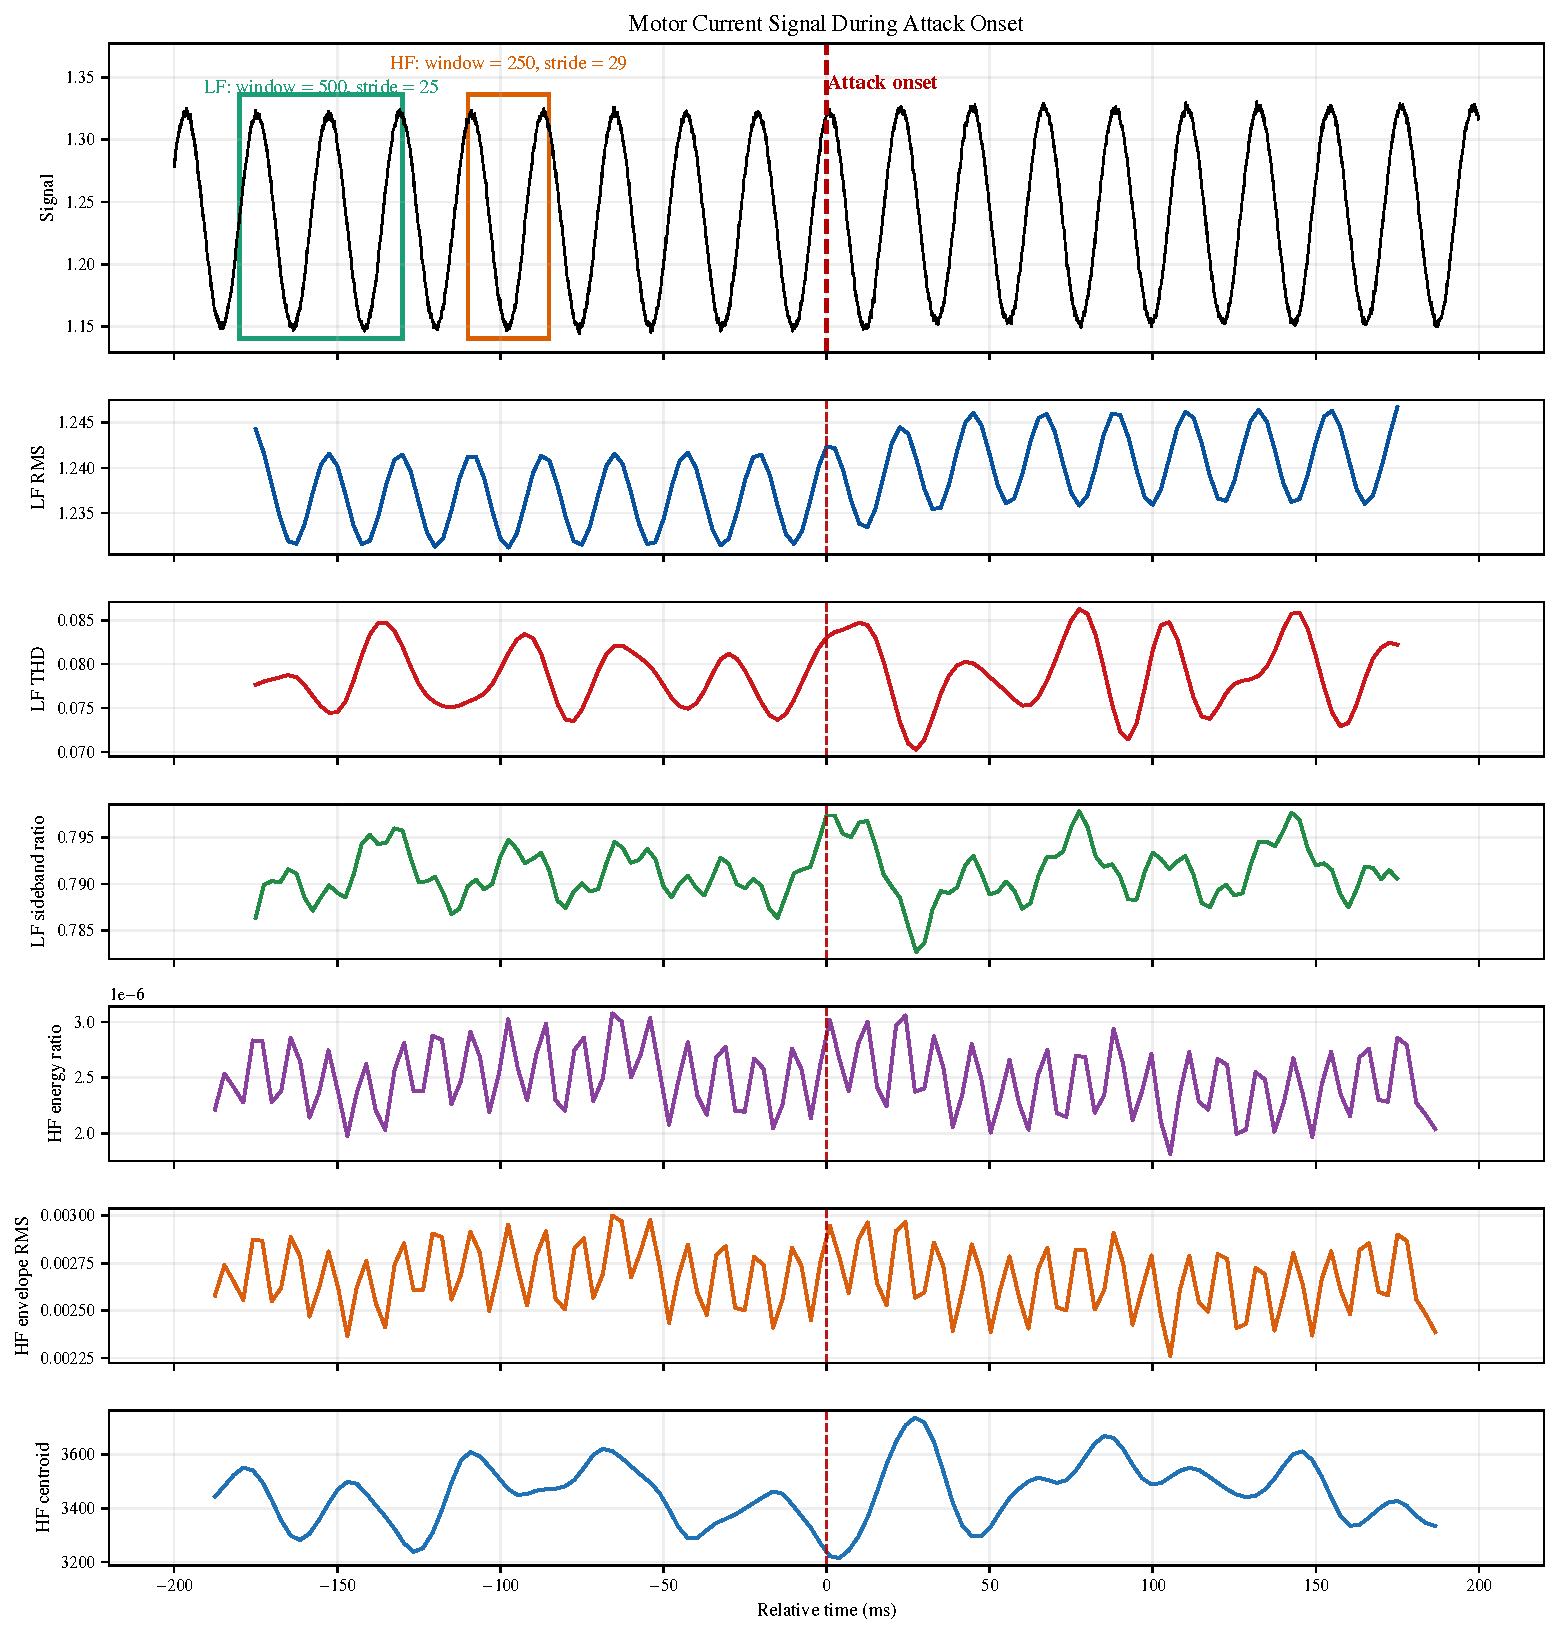
\includegraphics[viewport=52.29375000 33.49687500 741.04375000 107.71765625,clip,width=186bp,height=24bp]{figs_revised/original_sources/tdms_lfhf_window_example_acim_179p9s_separate.pdf}}
\put(62.00000,19){\color{black}\linethickness{0.3bp}\framebox(186,24){}}
\put(15.00000,31.00000){\makebox(0,0){\color{black}\fontsize{7.5bp}{8.5bp}\selectfont \shortstack{HF\\centroid\\(Hz)}}}
\put(59.00000,19.50550){\makebox(0,0)[r]{\color{black}\fontsize{7.5bp}{8.5bp}\selectfont 3200}}
\put(59.00000,36.19940){\makebox(0,0)[r]{\color{black}\fontsize{7.5bp}{8.5bp}\selectfont 3600}}
\put(70.45455,11.00000){\makebox(0,0){\color{black}\fontsize{7.5bp}{8.5bp}\selectfont -200}}
\put(112.73784,11.00000){\makebox(0,0){\color{black}\fontsize{7.5bp}{8.5bp}\selectfont -100}}
\put(155.02114,11.00000){\makebox(0,0){\color{black}\fontsize{7.5bp}{8.5bp}\selectfont 0}}
\put(197.30444,11.00000){\makebox(0,0){\color{black}\fontsize{7.5bp}{8.5bp}\selectfont 100}}
\put(239.58774,11.00000){\makebox(0,0){\color{black}\fontsize{7.5bp}{8.5bp}\selectfont 200}}
\put(148.00000,1.00000){\makebox(0,0){\color{black}\fontsize{8bp}{9bp}\selectfont Relative time (ms)}}
\put(155.02114,266.00000){\makebox(0,0){\color{red!70!black}\fontsize{8bp}{9bp}\selectfont Attack onset}}
\put(388.76000,286.00000){\makebox(0,0){\color{black}\fontsize{9bp}{10bp}\selectfont PCC current}}
\put(374.76000,274.00000){\makebox(0,0){\color{green!45!black}\fontsize{8bp}{9bp}\selectfont LF: 500/25}}
\put(454.76000,274.00000){\makebox(0,0){\color{orange!85!black}\fontsize{8bp}{9bp}\selectfont HF: 250/29}}
\put(324.76000,211){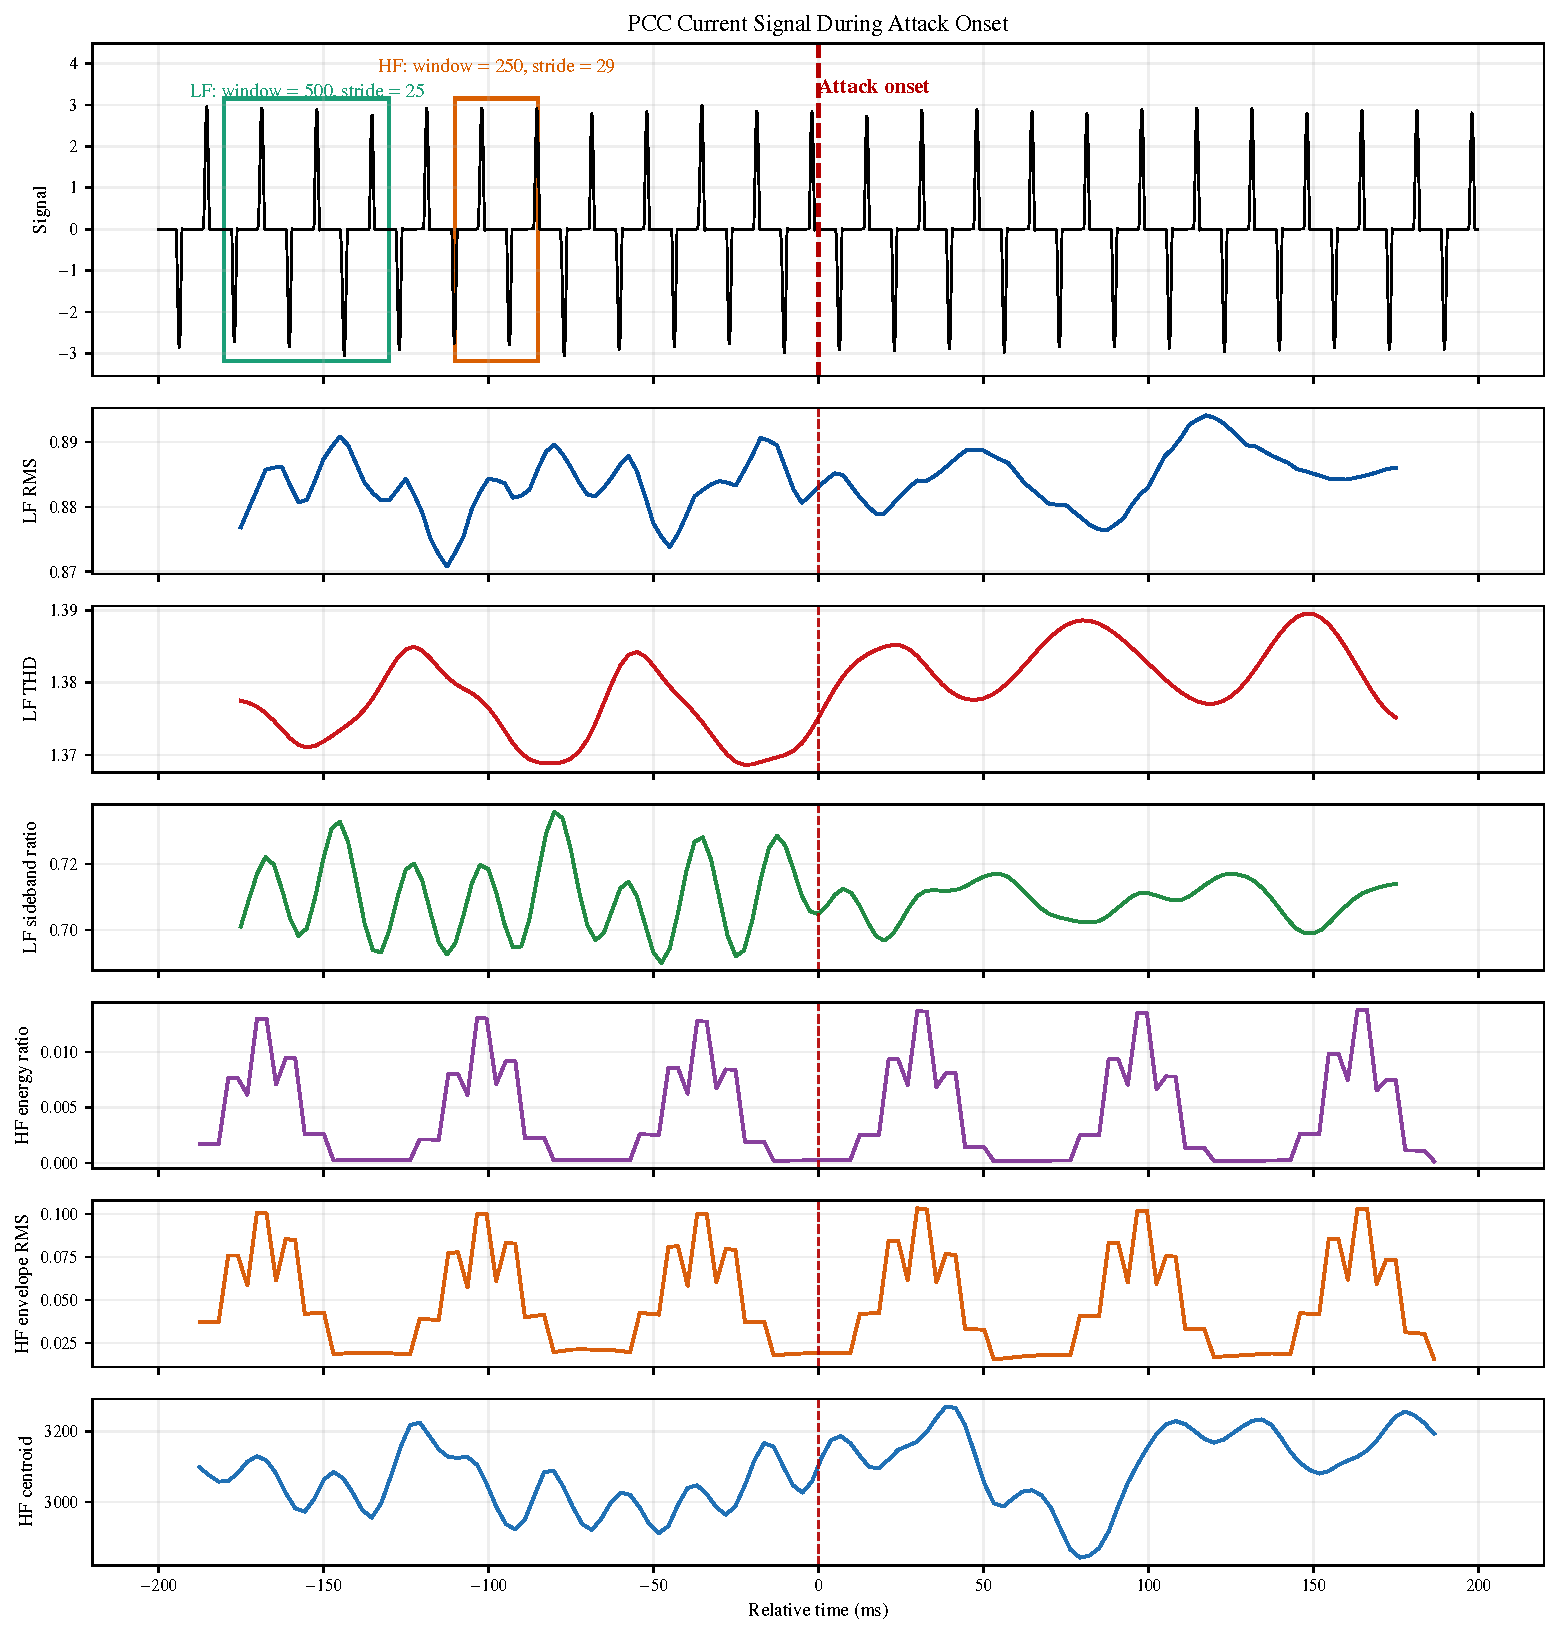
\includegraphics[viewport=44.30937500 604.36444980 741.06937500 764.00312500,clip,width=186bp,height=50bp]{figs_revised/original_sources/tdms_lfhf_window_example_pcc_179p9s_separate.pdf}}
\put(324.76000,211){\color{black}\linethickness{0.3bp}\framebox(186,50){}}
\put(277.76000,236.00000){\makebox(0,0){\color{black}\fontsize{7.5bp}{8.5bp}\selectfont \shortstack{Signal}}}
\put(321.76000,214.37135){\makebox(0,0)[r]{\color{black}\fontsize{7.5bp}{8.5bp}\selectfont -3}}
\put(321.76000,233.05698){\makebox(0,0)[r]{\color{black}\fontsize{7.5bp}{8.5bp}\selectfont 0}}
\put(321.76000,257.97114){\makebox(0,0)[r]{\color{black}\fontsize{7.5bp}{8.5bp}\selectfont 4}}
\put(324.76000,179){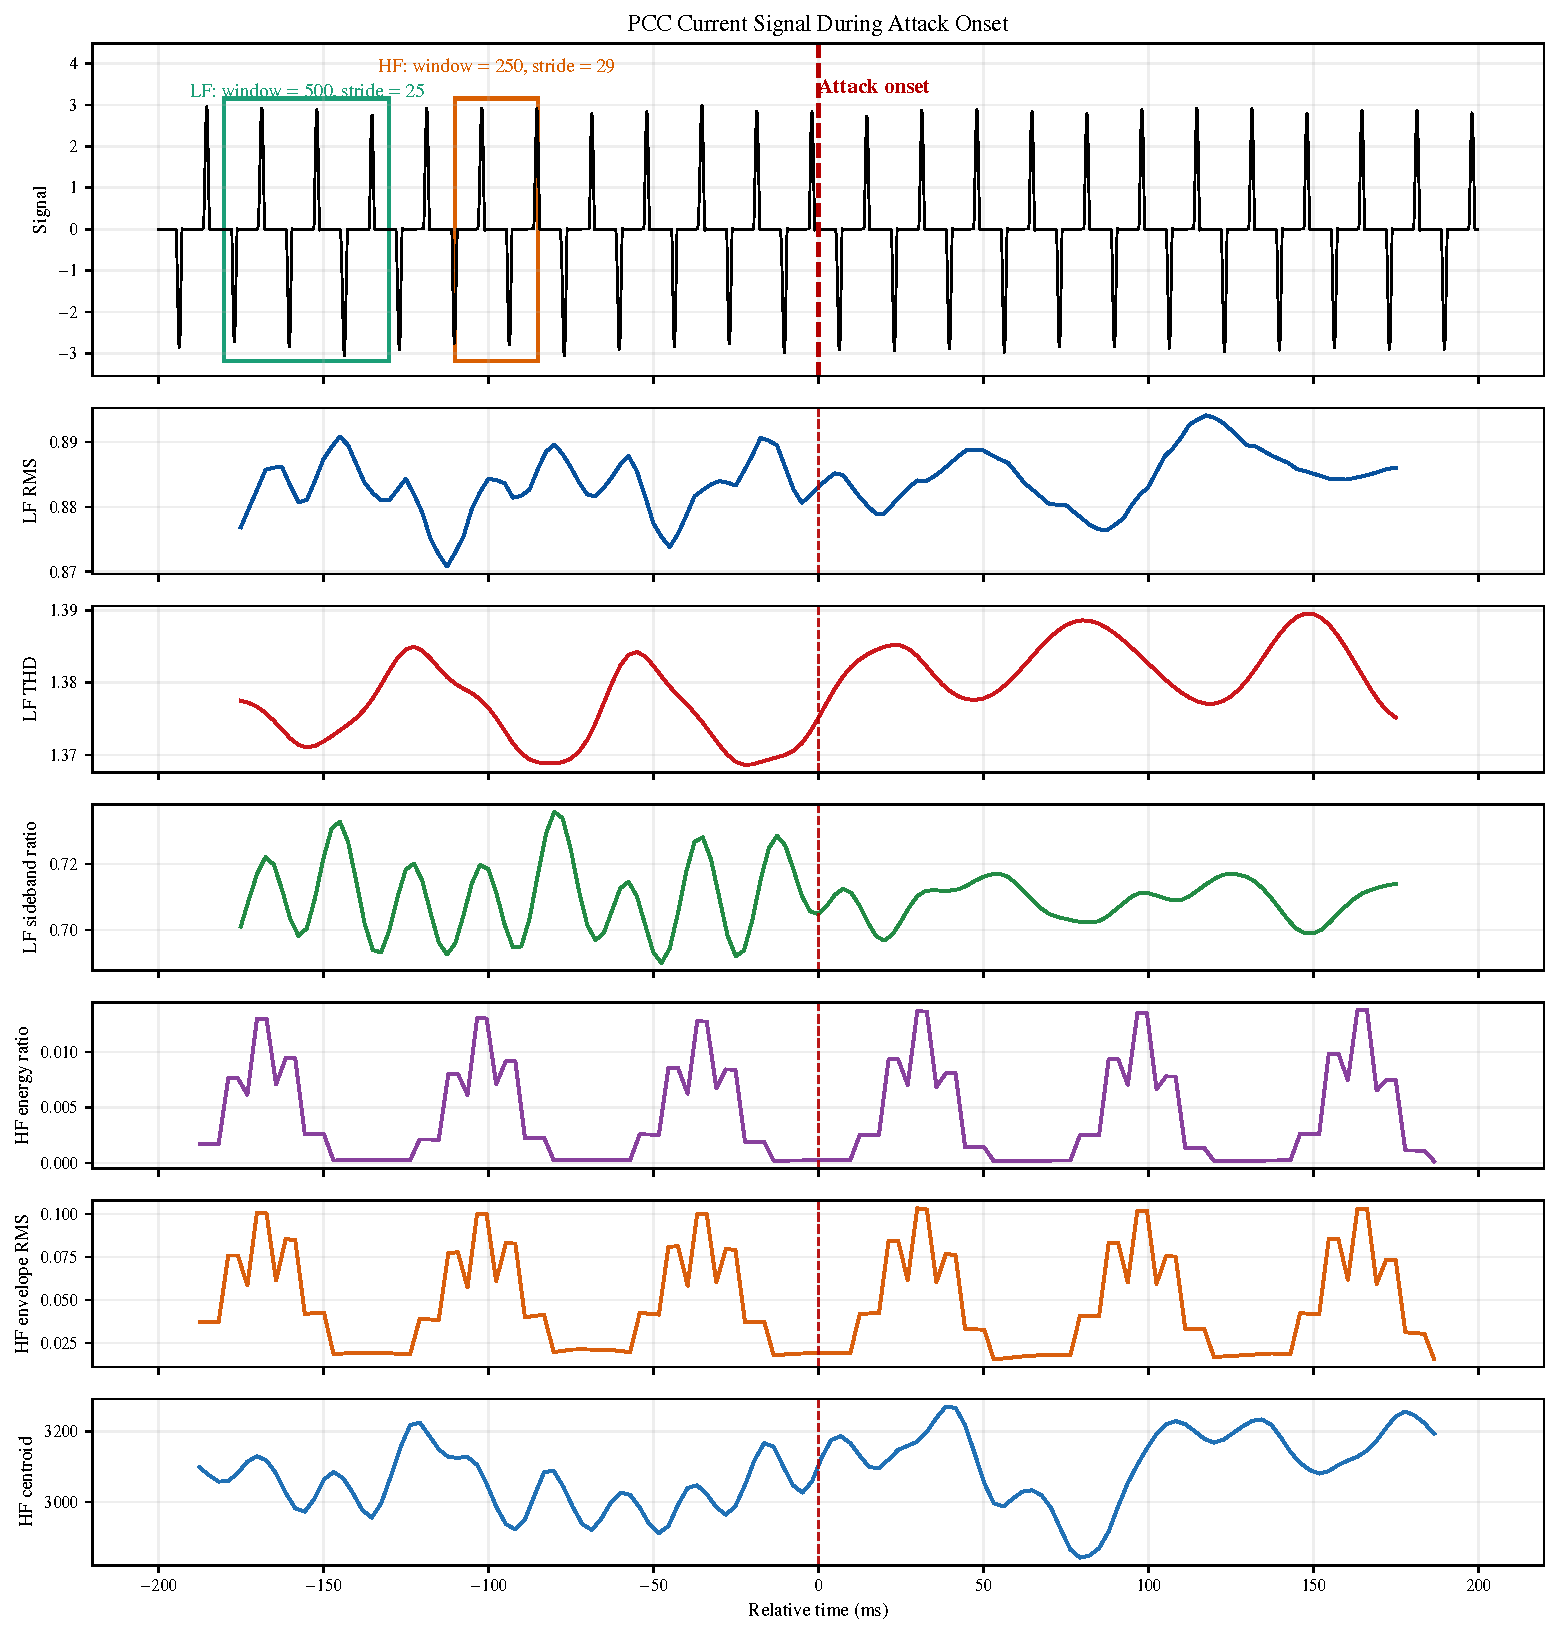
\includegraphics[viewport=44.30937500 509.21985400 741.06937500 589.03919160,clip,width=186bp,height=24bp]{figs_revised/original_sources/tdms_lfhf_window_example_pcc_179p9s_separate.pdf}}
\put(324.76000,179){\color{black}\linethickness{0.3bp}\framebox(186,24){}}
\put(277.76000,191.00000){\makebox(0,0){\color{black}\fontsize{7.5bp}{8.5bp}\selectfont \shortstack{LF\\RMS}}}
\put(321.76000,179.33480){\makebox(0,0)[r]{\color{black}\fontsize{7.5bp}{8.5bp}\selectfont 0.87}}
\put(321.76000,198.05361){\makebox(0,0)[r]{\color{black}\fontsize{7.5bp}{8.5bp}\selectfont 0.89}}
\put(324.76000,147){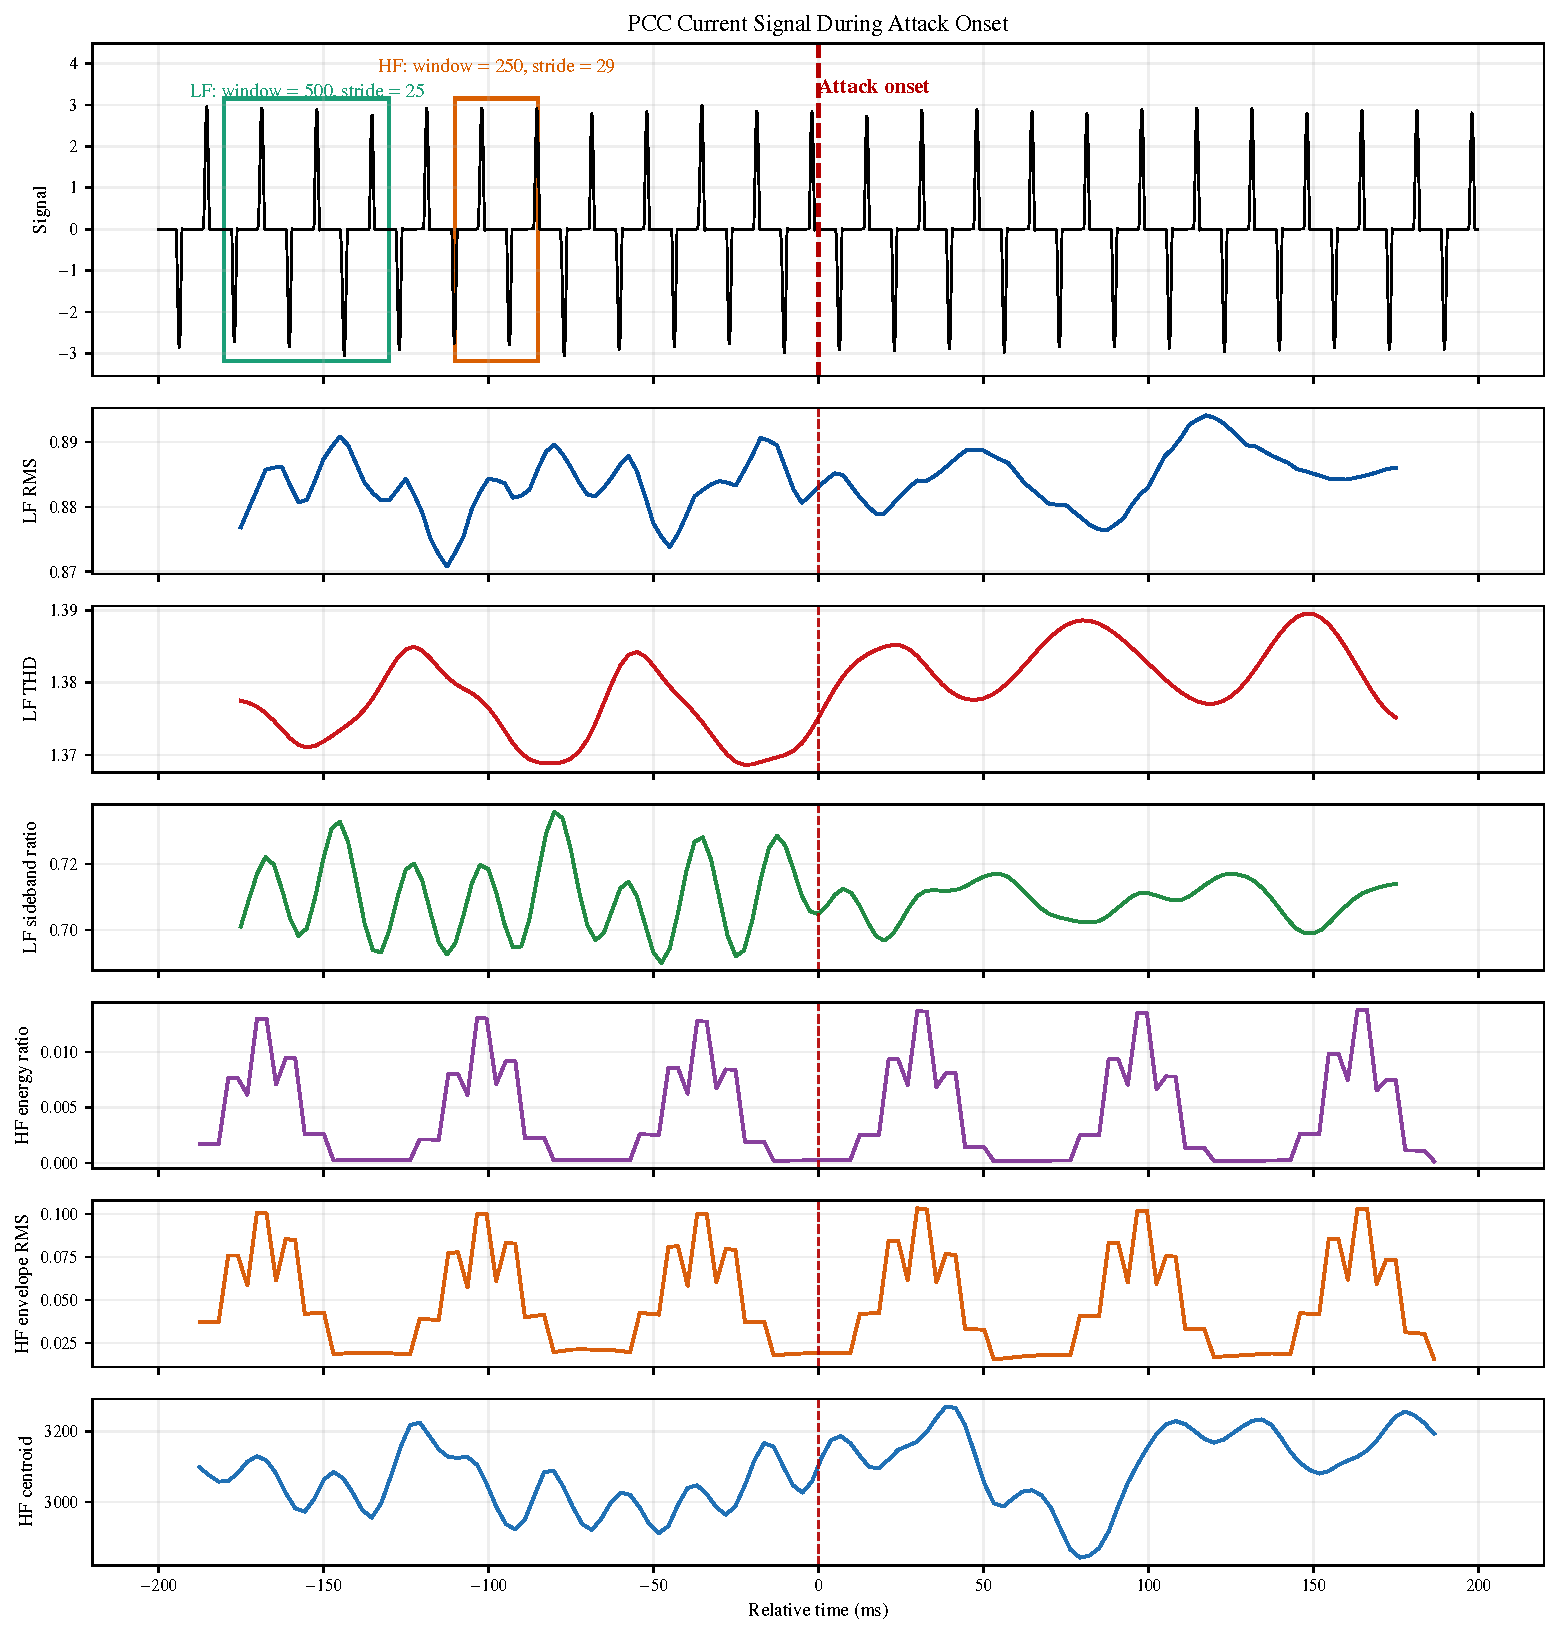
\includegraphics[viewport=44.30937500 414.07525820 741.06937500 493.89459580,clip,width=186bp,height=24bp]{figs_revised/original_sources/tdms_lfhf_window_example_pcc_179p9s_separate.pdf}}
\put(324.76000,147){\color{black}\linethickness{0.3bp}\framebox(186,24){}}
\put(277.76000,159.00000){\makebox(0,0){\color{black}\fontsize{7.5bp}{8.5bp}\selectfont \shortstack{LF\\THD}}}
\put(321.76000,149.51754){\makebox(0,0)[r]{\color{black}\fontsize{7.5bp}{8.5bp}\selectfont 1.37}}
\put(321.76000,170.36574){\makebox(0,0)[r]{\color{black}\fontsize{7.5bp}{8.5bp}\selectfont 1.39}}
\put(324.76000,115){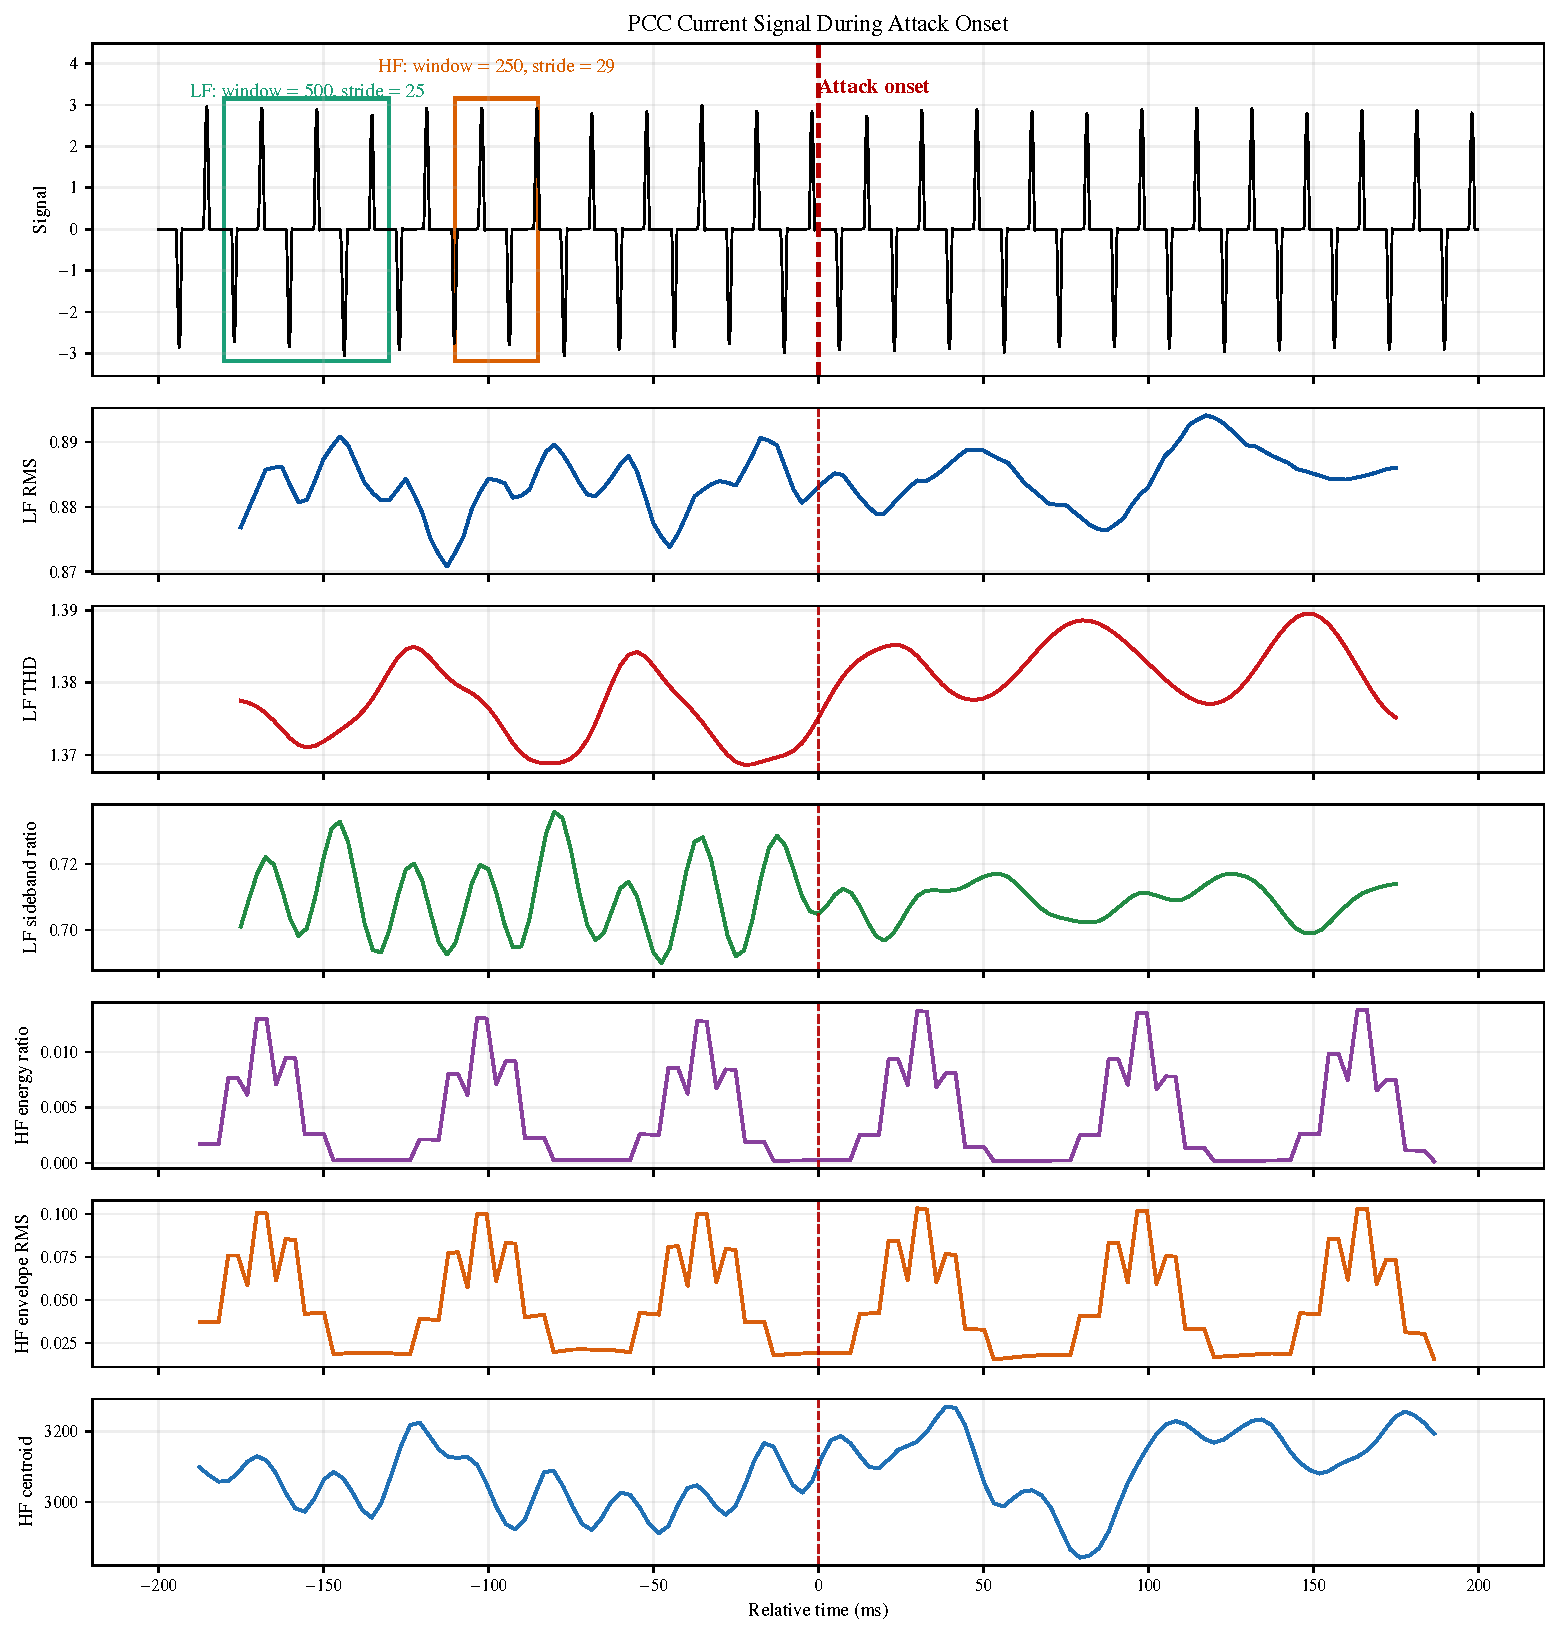
\includegraphics[viewport=44.30937500 318.93066240 741.06937500 398.75000000,clip,width=186bp,height=24bp]{figs_revised/original_sources/tdms_lfhf_window_example_pcc_179p9s_separate.pdf}}
\put(324.76000,115){\color{black}\linethickness{0.3bp}\framebox(186,24){}}
\put(277.76000,127.00000){\makebox(0,0){\color{black}\fontsize{7.5bp}{8.5bp}\selectfont \shortstack{LF\\sideband\\ratio}}}
\put(321.76000,120.83918){\makebox(0,0)[r]{\color{black}\fontsize{7.5bp}{8.5bp}\selectfont 0.70}}
\put(321.76000,130.40088){\makebox(0,0)[r]{\color{black}\fontsize{7.5bp}{8.5bp}\selectfont 0.72}}
\put(324.76000,83){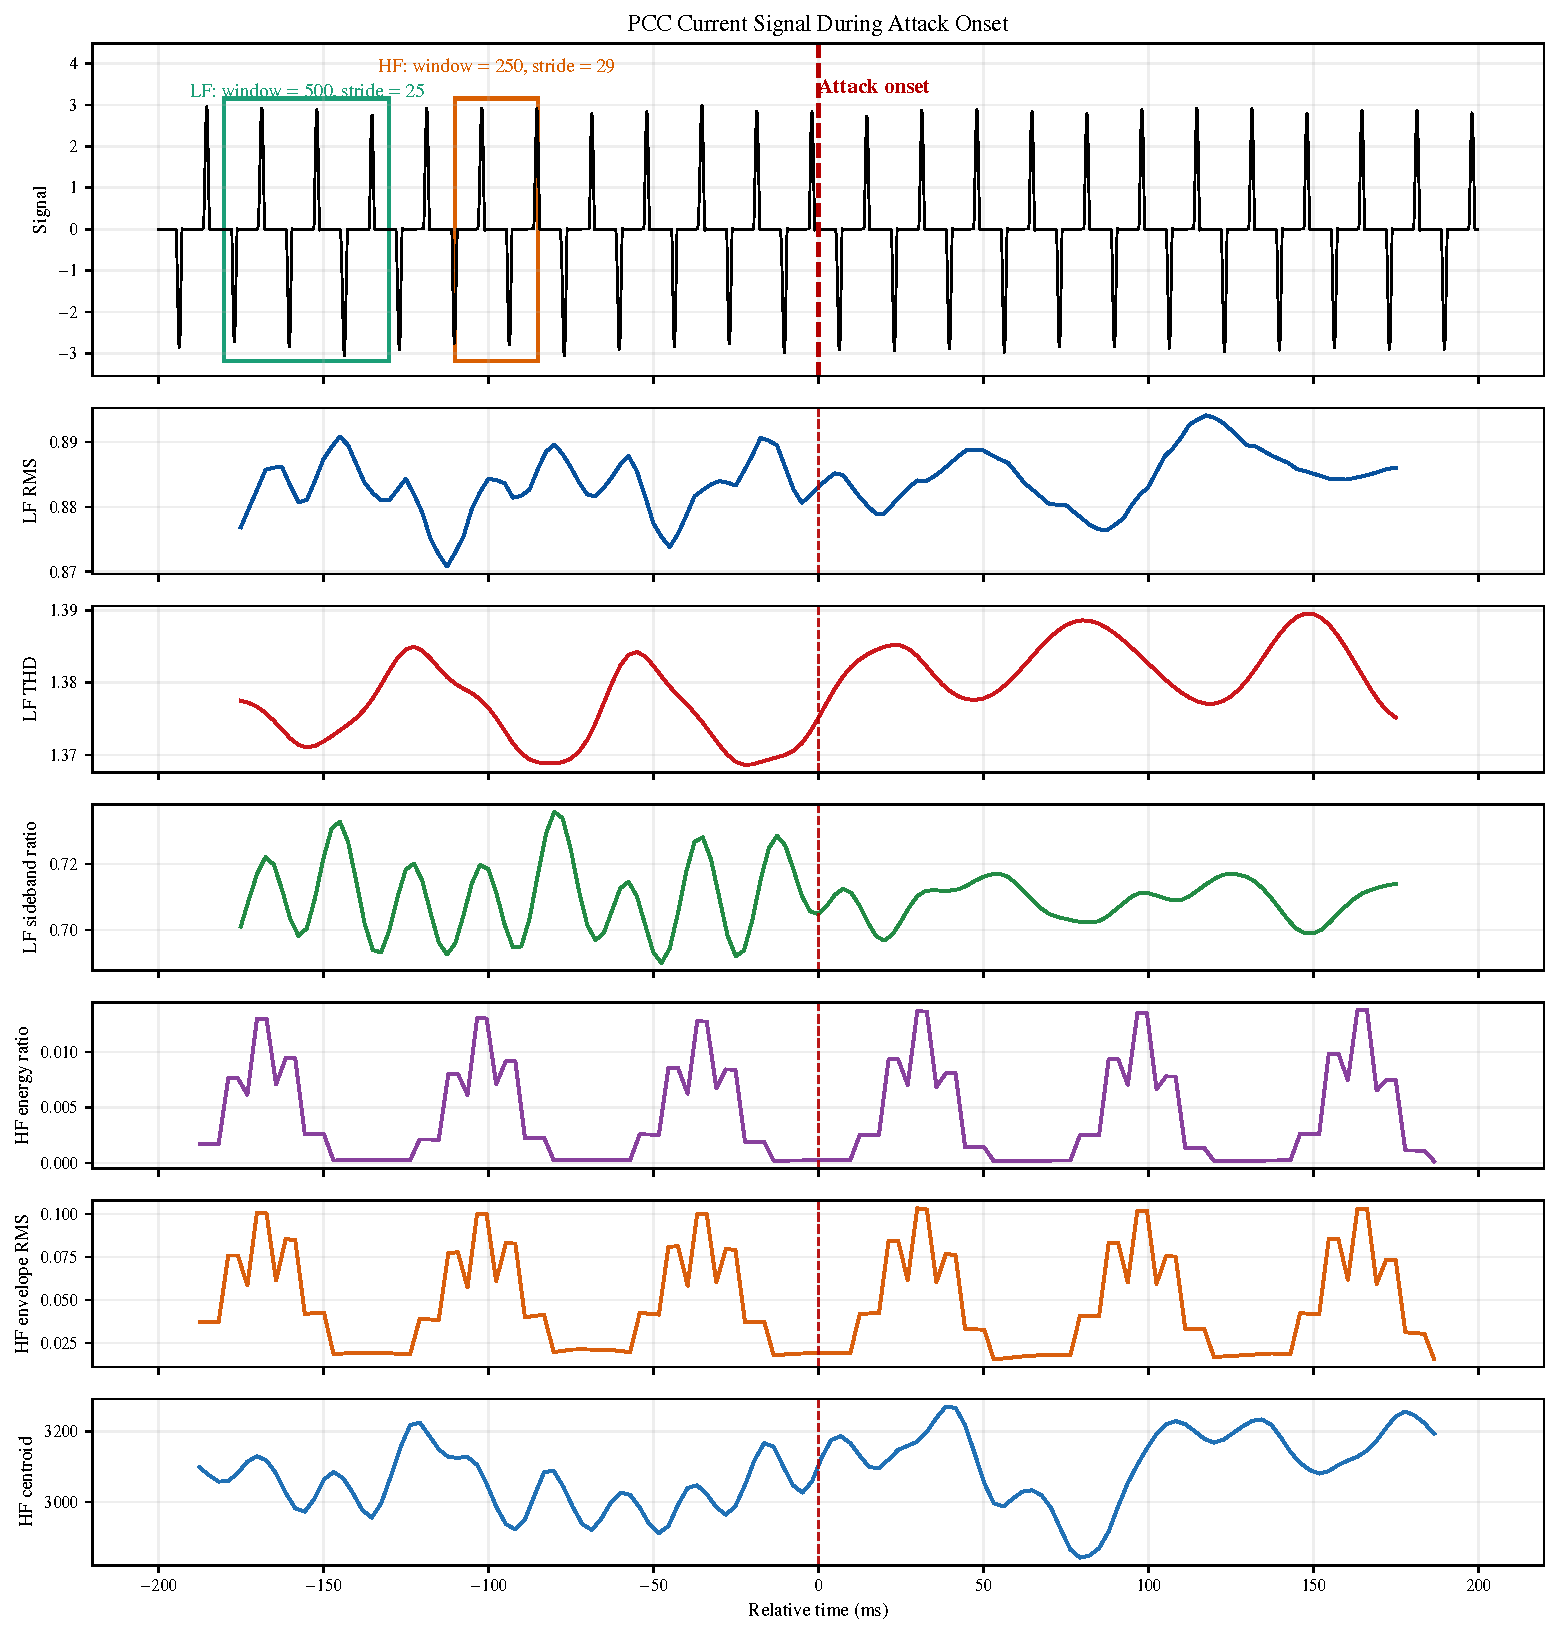
\includegraphics[viewport=44.30937500 223.78606660 741.06937500 303.60540420,clip,width=186bp,height=24bp]{figs_revised/original_sources/tdms_lfhf_window_example_pcc_179p9s_separate.pdf}}
\put(324.76000,83){\color{black}\linethickness{0.3bp}\framebox(186,24){}}
\put(277.76000,95.00000){\makebox(0,0){\color{black}\fontsize{7.5bp}{8.5bp}\selectfont \shortstack{HF energy\\ratio}}}
\put(321.76000,83.85710){\makebox(0,0)[r]{\color{black}\fontsize{7.5bp}{8.5bp}\selectfont 0.000}}
\put(321.76000,99.83159){\makebox(0,0)[r]{\color{black}\fontsize{7.5bp}{8.5bp}\selectfont 0.010}}
\put(324.76000,51){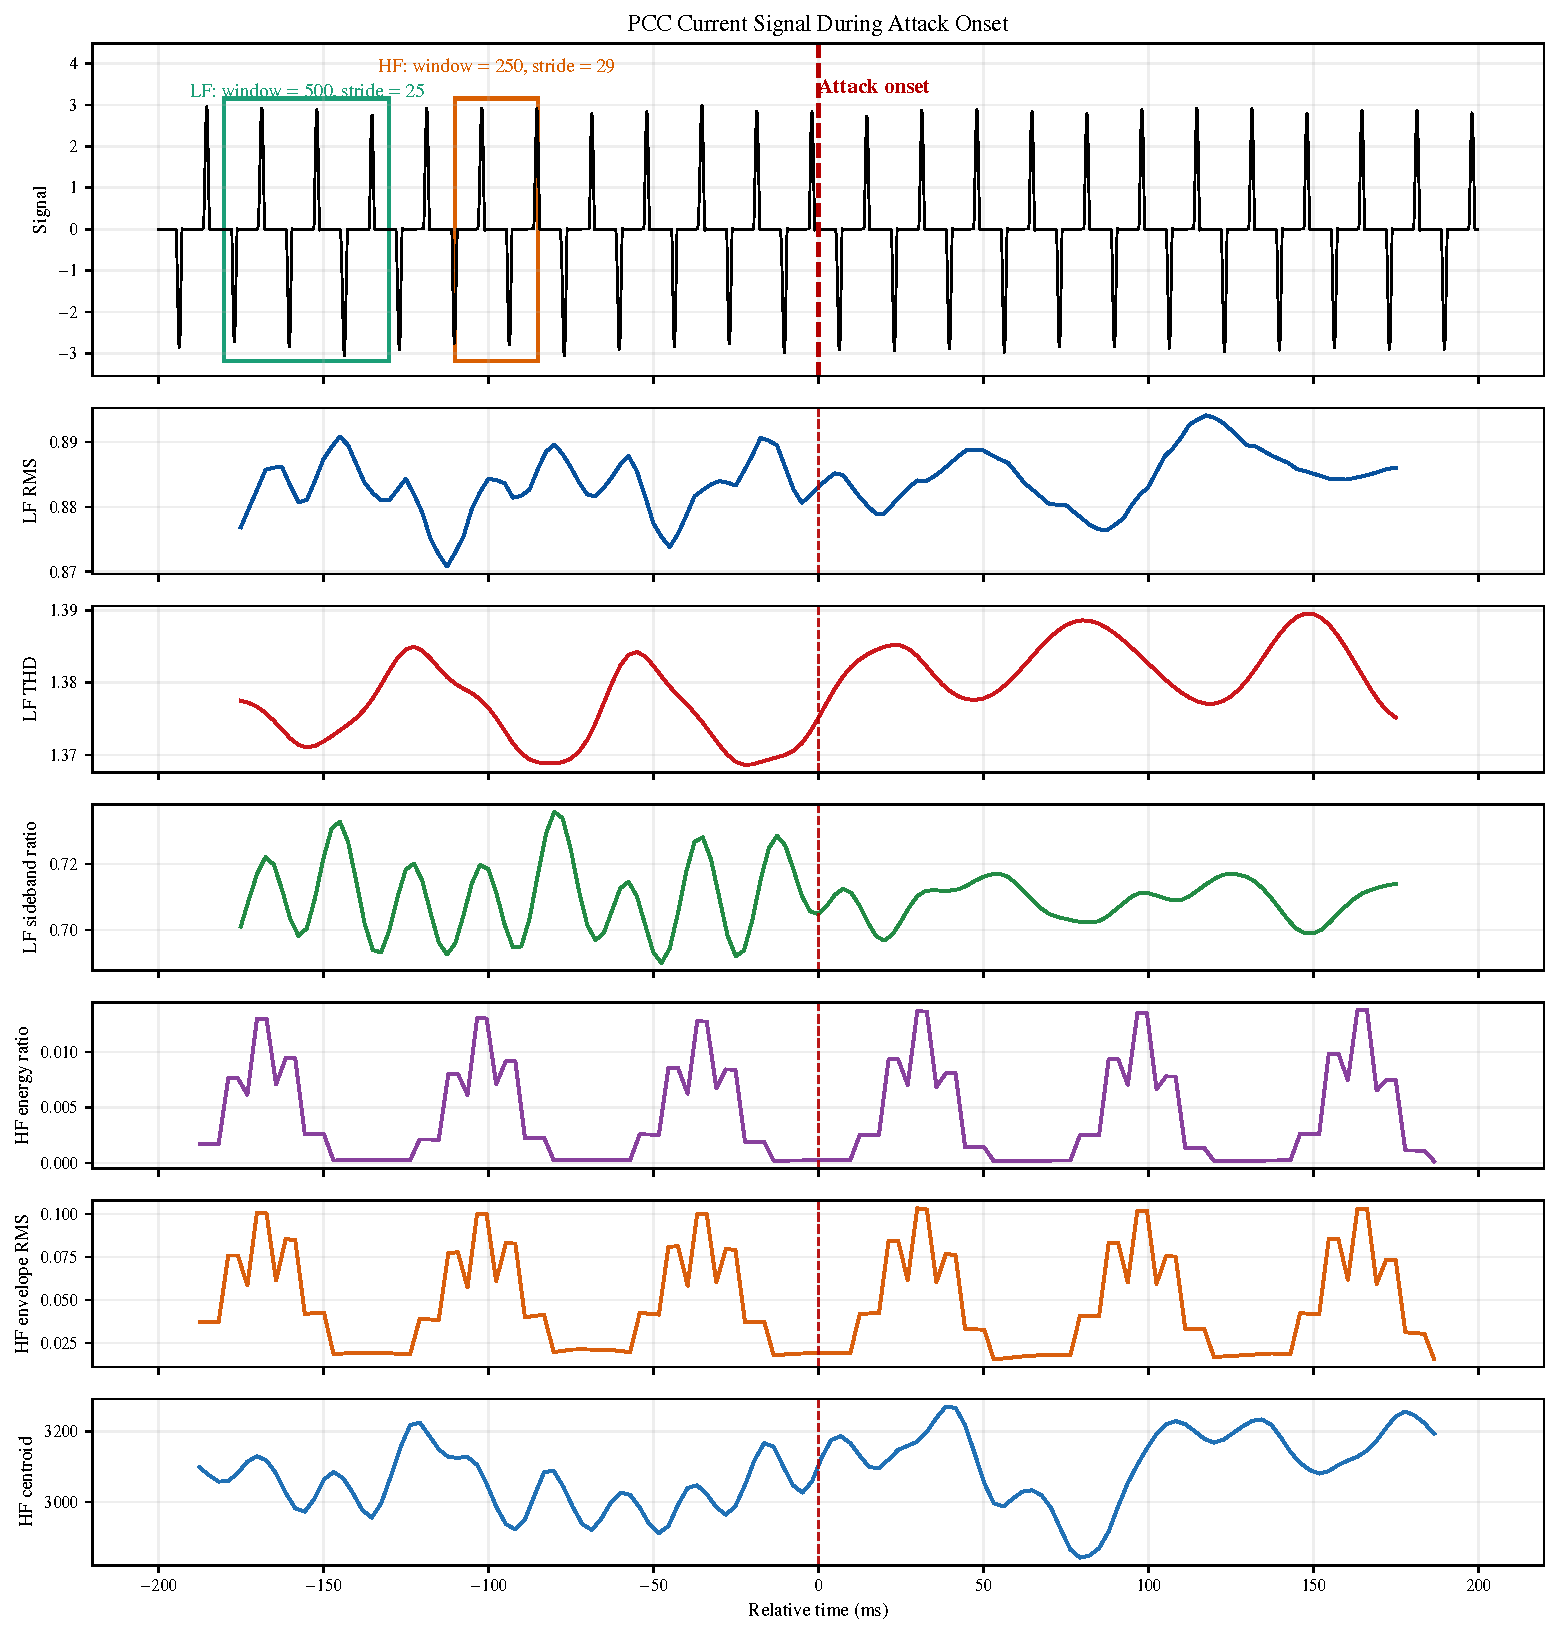
\includegraphics[viewport=44.30937500 128.64147080 741.06937500 208.46080840,clip,width=186bp,height=24bp]{figs_revised/original_sources/tdms_lfhf_window_example_pcc_179p9s_separate.pdf}}
\put(324.76000,51){\color{black}\linethickness{0.3bp}\framebox(186,24){}}
\put(277.76000,63.00000){\makebox(0,0){\color{black}\fontsize{7.5bp}{8.5bp}\selectfont \shortstack{HF\\envelope\\RMS}}}
\put(321.76000,54.48671){\makebox(0,0)[r]{\color{black}\fontsize{7.5bp}{8.5bp}\selectfont 0.025}}
\put(321.76000,73.07075){\makebox(0,0)[r]{\color{black}\fontsize{7.5bp}{8.5bp}\selectfont 0.100}}
\put(324.76000,19){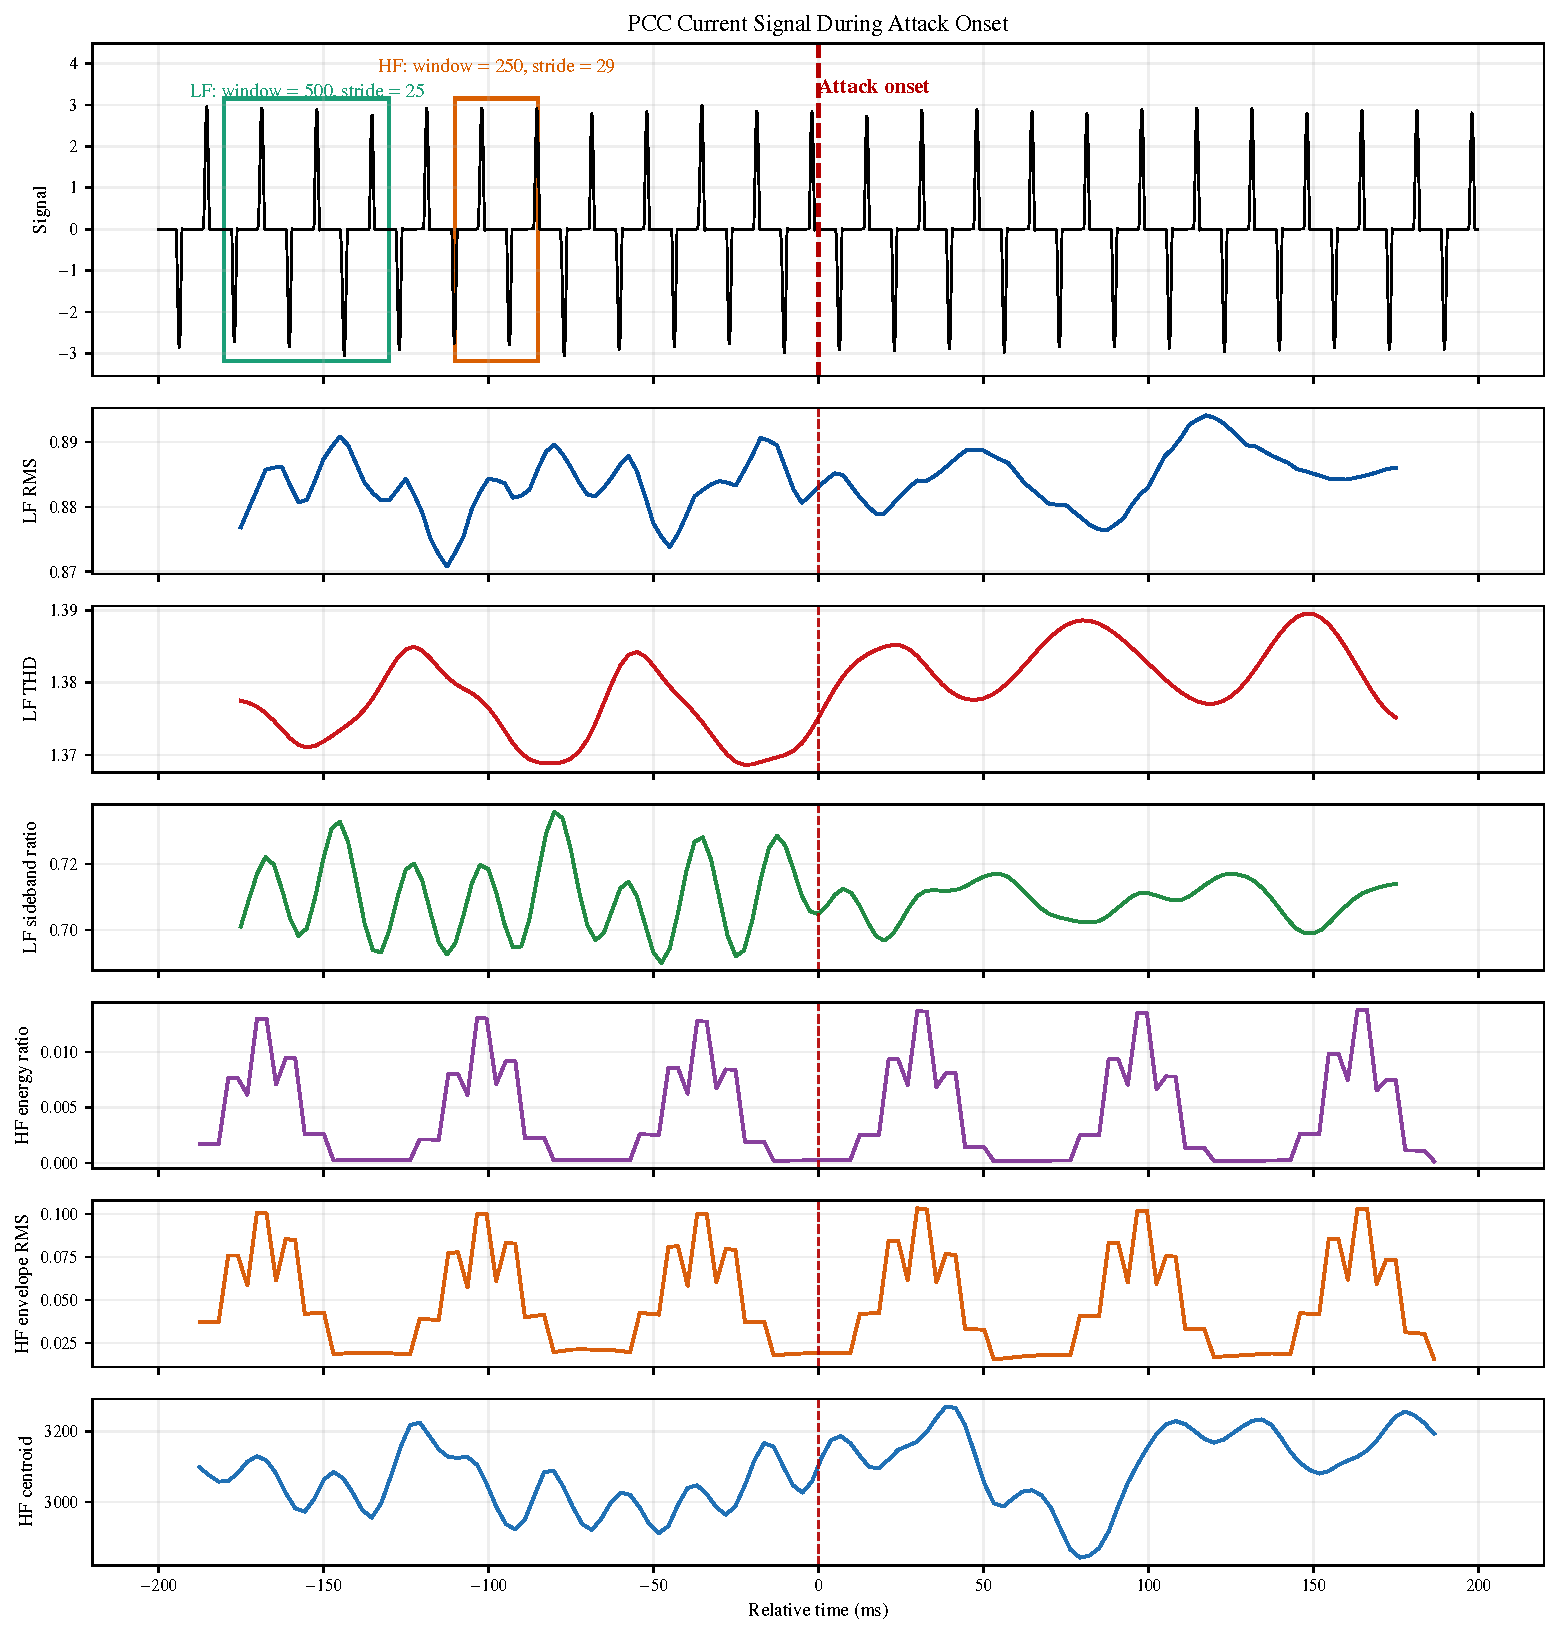
\includegraphics[viewport=44.30937500 33.49687500 741.06937500 113.31621260,clip,width=186bp,height=24bp]{figs_revised/original_sources/tdms_lfhf_window_example_pcc_179p9s_separate.pdf}}
\put(324.76000,19){\color{black}\linethickness{0.3bp}\framebox(186,24){}}
\put(277.76000,31.00000){\makebox(0,0){\color{black}\fontsize{7.5bp}{8.5bp}\selectfont \shortstack{HF\\centroid\\(Hz)}}}
\put(321.76000,28.13891){\makebox(0,0)[r]{\color{black}\fontsize{7.5bp}{8.5bp}\selectfont 3000}}
\put(321.76000,38.27264){\makebox(0,0)[r]{\color{black}\fontsize{7.5bp}{8.5bp}\selectfont 3200}}
\put(333.21455,11.00000){\makebox(0,0){\color{black}\fontsize{7.5bp}{8.5bp}\selectfont -200}}
\put(375.49784,11.00000){\makebox(0,0){\color{black}\fontsize{7.5bp}{8.5bp}\selectfont -100}}
\put(417.78114,11.00000){\makebox(0,0){\color{black}\fontsize{7.5bp}{8.5bp}\selectfont 0}}
\put(460.06444,11.00000){\makebox(0,0){\color{black}\fontsize{7.5bp}{8.5bp}\selectfont 100}}
\put(502.34774,11.00000){\makebox(0,0){\color{black}\fontsize{7.5bp}{8.5bp}\selectfont 200}}
\put(410.76000,1.00000){\makebox(0,0){\color{black}\fontsize{8bp}{9bp}\selectfont Relative time (ms)}}
\put(417.78114,266.00000){\makebox(0,0){\color{red!70!black}\fontsize{8bp}{9bp}\selectfont Attack onset}}
\end{picture}}
\endgroup
\caption{Representative motor-side and PCC-side signals at attack onset with the corresponding LF/HF feature responses.}
\label{fig:lfhf_motor_pcc_examples}

\end{minipage}
\end{minipage}
\end{adjustbox}
\end{figure*}






\begin{table*}[p]
\centering
\begin{adjustbox}{max width=\textwidth,max totalheight=0.87\textheight}
\begin{minipage}{\textwidth}
\centering
% Complete old block: tab:measurement_streams
\begin{minipage}[t]{0.48\textwidth}
\centering
\textcolor{red}{\textbf{ORIGINAL --- Table 2 (main.tex)}}\par\smallskip

\centering
\DiffOriginalCaption{Table 2: Measurement streams used for monitoring.}

\renewcommand{\arraystretch}{1.15}
\begin{adjustbox}{max width=\linewidth}\begin{tabular}{l c c}
\hline
Stream & Measured signals & Channels \\
\hline
Motor-side & ACIM and PMSM phase currents & 6 \\
PCC-side   & PCC voltage and current & 2 \\
\hline
\end{tabular}\end{adjustbox}

\end{minipage}\hfill%
% Complete new block: tab:measurement_streams
\begin{minipage}[t]{0.48\textwidth}
\centering
\textcolor{blue}{\textbf{REVISED --- Table 2 (main\_revised.tex)}}\par\smallskip

\centering
\caption{Measurement streams used for monitoring.}
\label{tab:measurement_streams}
\renewcommand{\arraystretch}{1.15}
\begin{tabular}{l c c}
\hline
Stream & Measured signals & Channels \\
\hline
Motor-side & ACIM and PMSM phase currents & 6 \\
PCC-side   & PCC voltage and current & 2 \\
\hline
\end{tabular}

\end{minipage}
\end{minipage}
\end{adjustbox}
\end{table*}






\begin{table*}[p]
\centering
\begin{adjustbox}{max width=\textwidth,max totalheight=0.87\textheight}
\begin{minipage}{\textwidth}
\centering
% Complete old block: tab:evaluation_protocols
\begin{minipage}[t]{0.48\textwidth}
\centering
\textcolor{red}{\textbf{ORIGINAL --- Table 3 (main.tex)}}\par\smallskip

\centering
\DiffOriginalCaption{Table 3: Dataset dimensions and evaluation protocols.}

\footnotesize
\renewcommand{\arraystretch}{1.15}
\setlength{\tabcolsep}{3.5pt}
\begin{adjustbox}{max width=\linewidth}\begin{tabularx}{\columnwidth}{@{}p{0.38\columnwidth}X@{}}
\toprule
\textbf{Parameter} & \textbf{Value / Configuration} \\
\hline
\multicolumn{2}{c}{\textit{Data dimensions}} \\
\hline
Total samples       & 60,054 \\
Motor distribution  & ACIM: 30,204; PMSM: 29,850 \\
Binary distribution & Normal: 33,054; Attack: 27,000 \\

\hline
\multicolumn{2}{c}{\textit{Input configuration}} \\
\hline
Time steps per sample, $W$ & 61 \\
Features per channel       & 37 \\
Channels                   & Motor: 6; PCC: 2 \\
Motor feature shape         & $(N,W,F)=(N,61,222)$ \\
PCC feature shape           & $(N,W,F)=(N,61,74)$ \\
\hline
\multicolumn{2}{c}{\textit{Severity labels}} \\
\hline
Raw severity levels & $0\%, 0.05\%, 0.1\%, \ldots, 0.5\%$ \\
Four-class labels   & Normal: 33,054; Mild: 8,100; Medium: 10,800; Severe: 8,100 \\

\hline
\multicolumn{2}{c}{\textit{Protocol 1: In-domain evaluation}} \\
\hline
Split ratio    & Train / validation / test = 70\% / 15\% / 15\% \\
Sample counts  & 42,037 / 9,008 / 9,009 \\
Domain composition & ACIM and PMSM samples appear in all splits \\

\hline
\multicolumn{2}{c}{\textit{Protocol 2: Cross-domain evaluation}} \\
\hline
Transfer directions & ACIM $\rightarrow$ PMSM; PMSM $\rightarrow$ ACIM \\
Adaptation ratios   & 1\%, 5\%, 10\%, and 20\% labeled target data \\
Reporting           & Three seeds; accuracy and balanced accuracy \\

\bottomrule
\end{tabularx}\end{adjustbox}

\end{minipage}\hfill%
% Complete new block: tab:evaluation_protocols
\begin{minipage}[t]{0.48\textwidth}
\centering
\textcolor{blue}{\textbf{REVISED --- Table 3 (main\_revised.tex)}}\par\smallskip

\centering
\footnotesize
\caption{Dataset dimensions and recording-disjoint
evaluation protocols.}
\label{tab:evaluation_protocols}
\renewcommand{\arraystretch}{1.10}
\setlength{\tabcolsep}{2pt}

\begin{tabular}{@{}p{0.36\columnwidth}p{0.60\columnwidth}@{}}
\hline
Parameter & Value / configuration \\
\hline
\multicolumn{2}{c}{\textit{Data dimensions}} \\
\hline
Complete windows & 60,054; 2,000 samples (0.2 s) each \\
Recordings / episodes & 18 recordings; 540 scheduled episodes \\
Motor distribution & ACIM: 30,204; PMSM: 29,850 \\
Normal / attack windows & 33,054 normal; 27,000 attack \\

\hline
\multicolumn{2}{c}{\textit{Input configuration}} \\
\hline
Features per channel & 37 (18 LF, 11 HF, 8 TD) \\
Time steps, $W$ & 61 \\
Channels & Motor: 6; PCC: 2 \\
Motor input shape & $(N,61,222)$ \\
PCC input shape & $(N,61,74)$ \\

\hline
\multicolumn{2}{c}{\textit{Severity labels (\texttt{severity4})}} \\
\hline
Normal / low & 33,054 / 5,400 windows \\
Medium / high & 7,200 / 14,400 windows \\

\hline
\multicolumn{2}{c}{\textit{Protocol 1: mixed-motor holdouts}} \\
\hline
Recordings per motor & 5 train; 2 val.; 2 test \\
Window count order & Train / Val. / Test \\
Repeat 1 (1234) & 33,718 / 13,279 / 13,057 \\
Repeat 2 (2234) & 33,275 / 13,250 / 13,529 \\
Repeat 3 (3234) & 33,560 / 13,227 / 13,267 \\

\hline
\multicolumn{2}{c}{\textit{Protocol 2: cross-motor adaptation}} \\
\hline
Transfer directions &
ACIM $\rightarrow$ PMSM;
PMSM $\rightarrow$ ACIM \\
Target recordings &
6 adaptation-pool; 3 held-out test \\
Adaptation budgets &
1/5/10/20\% $\rightarrow$ 2/9/18/36
complete episode groups (out of 180) \\
\hline
\end{tabular}

\par\smallskip
\begin{minipage}{\columnwidth}
\scriptsize
Each recording and all its episodes remain in one
partition within a repeat. $N$: number of windows.
\end{minipage}

\end{minipage}
\end{minipage}
\end{adjustbox}
\end{table*}
\DIFaddend




\section{The Proposed Method}
\label{sec:method}

\DIFdelbegin \subsection{\DIFdel{LF/HF Feature Extraction Pipeline}}
%DIFAUXCMD
\addtocounter{subsection}{-1}%DIFAUXCMD
%DIFDELCMD < \label{sec:lfhf_features}
%DIFDELCMD <

%DIFDELCMD < %%%
\DIFdelend To represent both slow electromechanical behavior and faster attack-induced disturbances, a two-scale LF/HF feature pipeline was applied independently to each \DIFdelbegin \DIFdel{current channel. }\DIFdelend \DIFaddbegin \DIFadd{measured channel. Separate classifiers use these features for attack detection, motor localization, and injected-bias severity assessment.
}

\subsection{\DIFadd{LF/HF Feature Extraction Pipeline}}
\label{sec:lfhf_features}

\DIFaddend For every sample, a 2{,}000-point outer window was first extracted from the raw 10~kHz recording. Within this outer window, two parallel sliding analyses were performed. The LF branch uses a 500-sample window with a stride of 25 samples, while the HF branch uses a 250-sample window with a stride of 29 samples. The LF and HF settings both produce 61 time steps, enabling concatenation into one temporal feature tensor.
Fig.~\ref{fig:lfhf_motor_pcc_examples} illustrates representative attack-onset responses and the corresponding LF/HF windows. In both cases, the raw signal is shown around the attack-transition instant, and representative LF and HF windows are overlaid to illustrate the two-scale extraction procedure. \DIFdelbegin \DIFdel{The motor-side signals exhibit stronger and more localized variations, whereas PCC-side responses are more distributed due to their aggregated nature}\DIFdelend \DIFaddbegin \DIFadd{Signal amplitudes are in recorded acquisition units}\DIFaddend .


In total, 37 features were extracted per channel, including 18 LF spectral features, 11 HF spectral/envelope features, and 8 TD features. The LF branch targets slow electromechanical changes, fundamental-frequency behavior, harmonic distortion, sideband effects, and low-band energy redistribution. The HF branch captures higher-frequency redistribution and envelope-related changes that may appear during small current-feedback FDIAs. The TD features provide complementary sensitivity to amplitude variation, impulsiveness, waveform asymmetry, and short-term signal complexity.
Together, these features \DIFaddbegin \DIFadd{help }\DIFaddend make weak PCC FDIA signatures more separable despite harmonics, grid interaction, and aggregation.

\subsection{Inception-Based Detection Model}
\label{sec:inception_model}

The extracted LF/HF tensors were modeled using a one-dimensional InceptionTime architecture~\cite{fawaz2020inceptiontime} for multivariate time-series classification. The input dimension is $(61,222)$ for the motor stream and $(61,74)$ for the PCC stream. As illustrated in Fig.~\ref{fig:inceptiontime_architecture}, the network uses bottleneck compression, parallel one-dimensional convolutional kernels \DIFaddbegin \DIFadd{of lengths 39, 19, and 9}\DIFaddend , residual shortcuts, global average pooling, and a dense output layer. Motor and PCC models used stream-specific hyperparameters selected by validation balanced accuracy. \DIFdelbegin \DIFdel{The Inception-based design is well suited to the proposed LF/HF representation because the extracted features retain temporal ordering across the 61-step sequence. This preserves temporal interactions among LF, HF, and TD features}\DIFdelend \DIFaddbegin \DIFadd{Each task uses a separately trained model with two outputs for }\texttt{\DIFadd{fdia2}}\DIFadd{, three for }\texttt{\DIFadd{fdia3}}\DIFadd{, and four for }\texttt{\DIFadd{severity4}}\DIFaddend .



\DIFaddbegin \begin{figure*}[p]
\centering
\begin{adjustbox}{max width=\textwidth,max totalheight=0.87\textheight}
\begin{minipage}{\textwidth}
\centering
% Complete old block: fig:inceptiontime_architecture
\begin{minipage}[t]{\textwidth}
\centering
\textcolor{red}{\textbf{ORIGINAL --- Figure 3 (main.tex)}}\par\smallskip

    \centering
    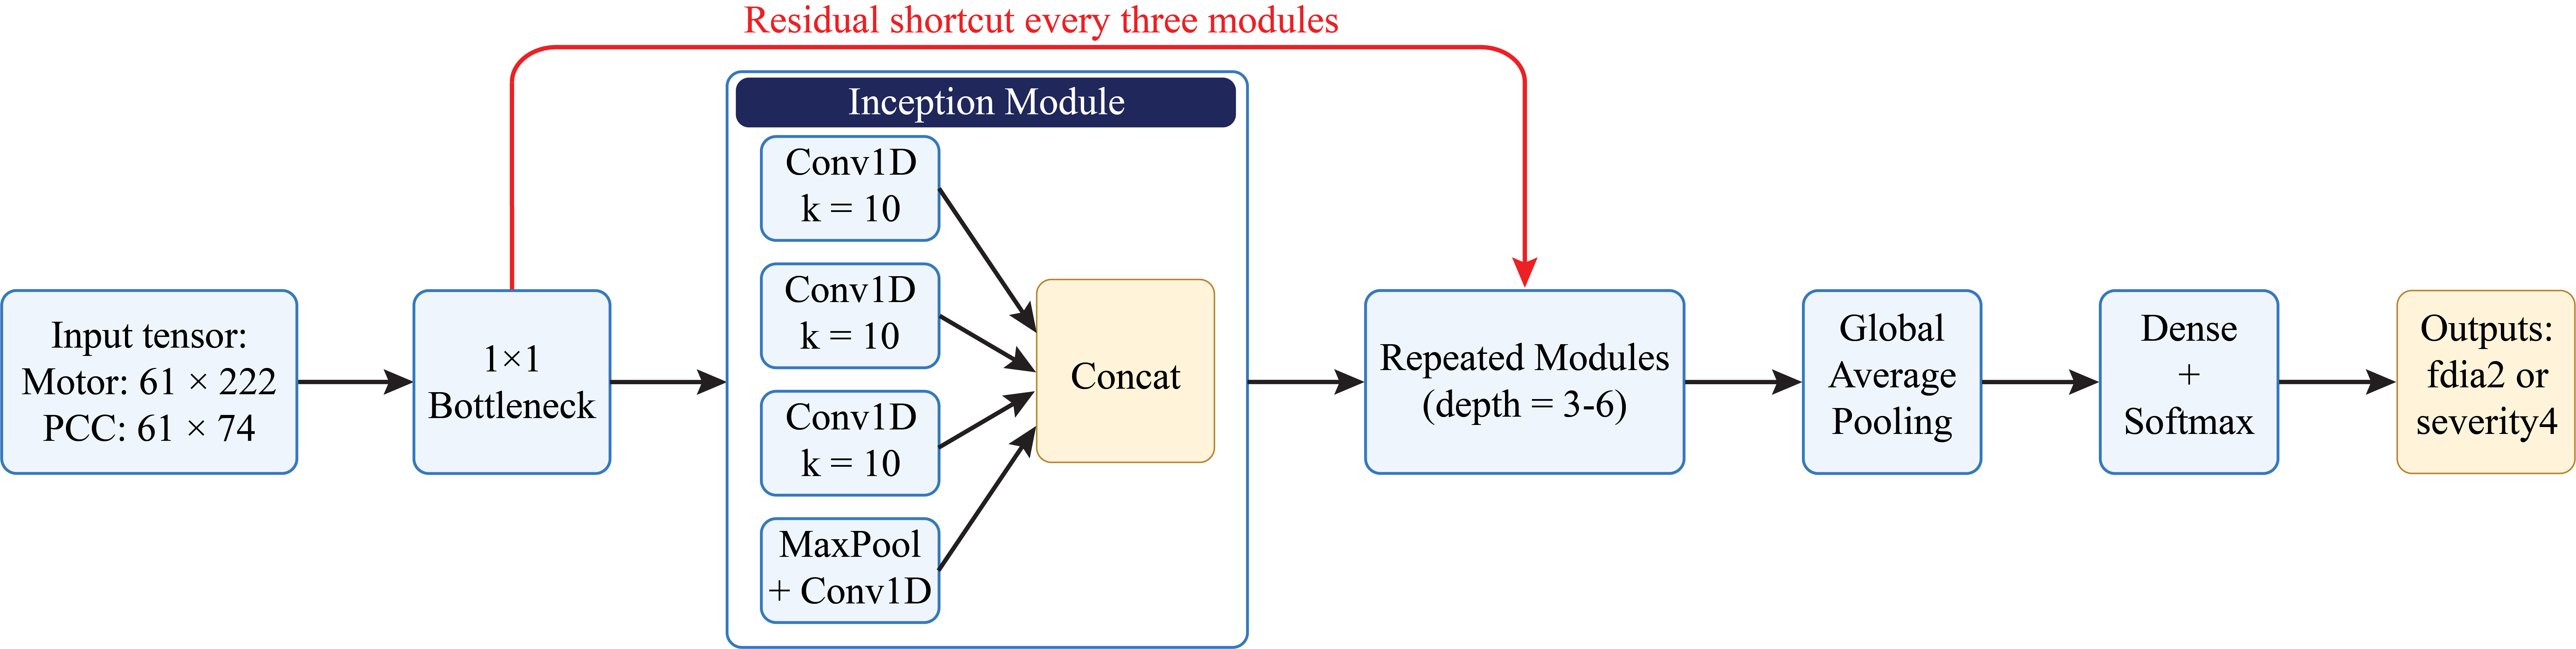
\includegraphics[width=0.95\textwidth]{figs/inceptiontime_architecture_lfhf.png}
    \DiffOriginalCaption{Figure 3: Overview of the InceptionTime-based classifier used for \texttt{fdia2} detection and \texttt{severity4} classification.}


\end{minipage}\par\vspace{1em}
% Complete new block: fig:inceptiontime_architecture
\begin{minipage}[t]{\textwidth}
\centering
\textcolor{blue}{\textbf{REVISED --- Figure 3 (main\_revised.tex)}}\par\smallskip

\centering
\begingroup
\setlength{\unitlength}{1bp}
\resizebox{\linewidth}{!}{\begin{picture}(515.5200,129.8992)

\put(0,0){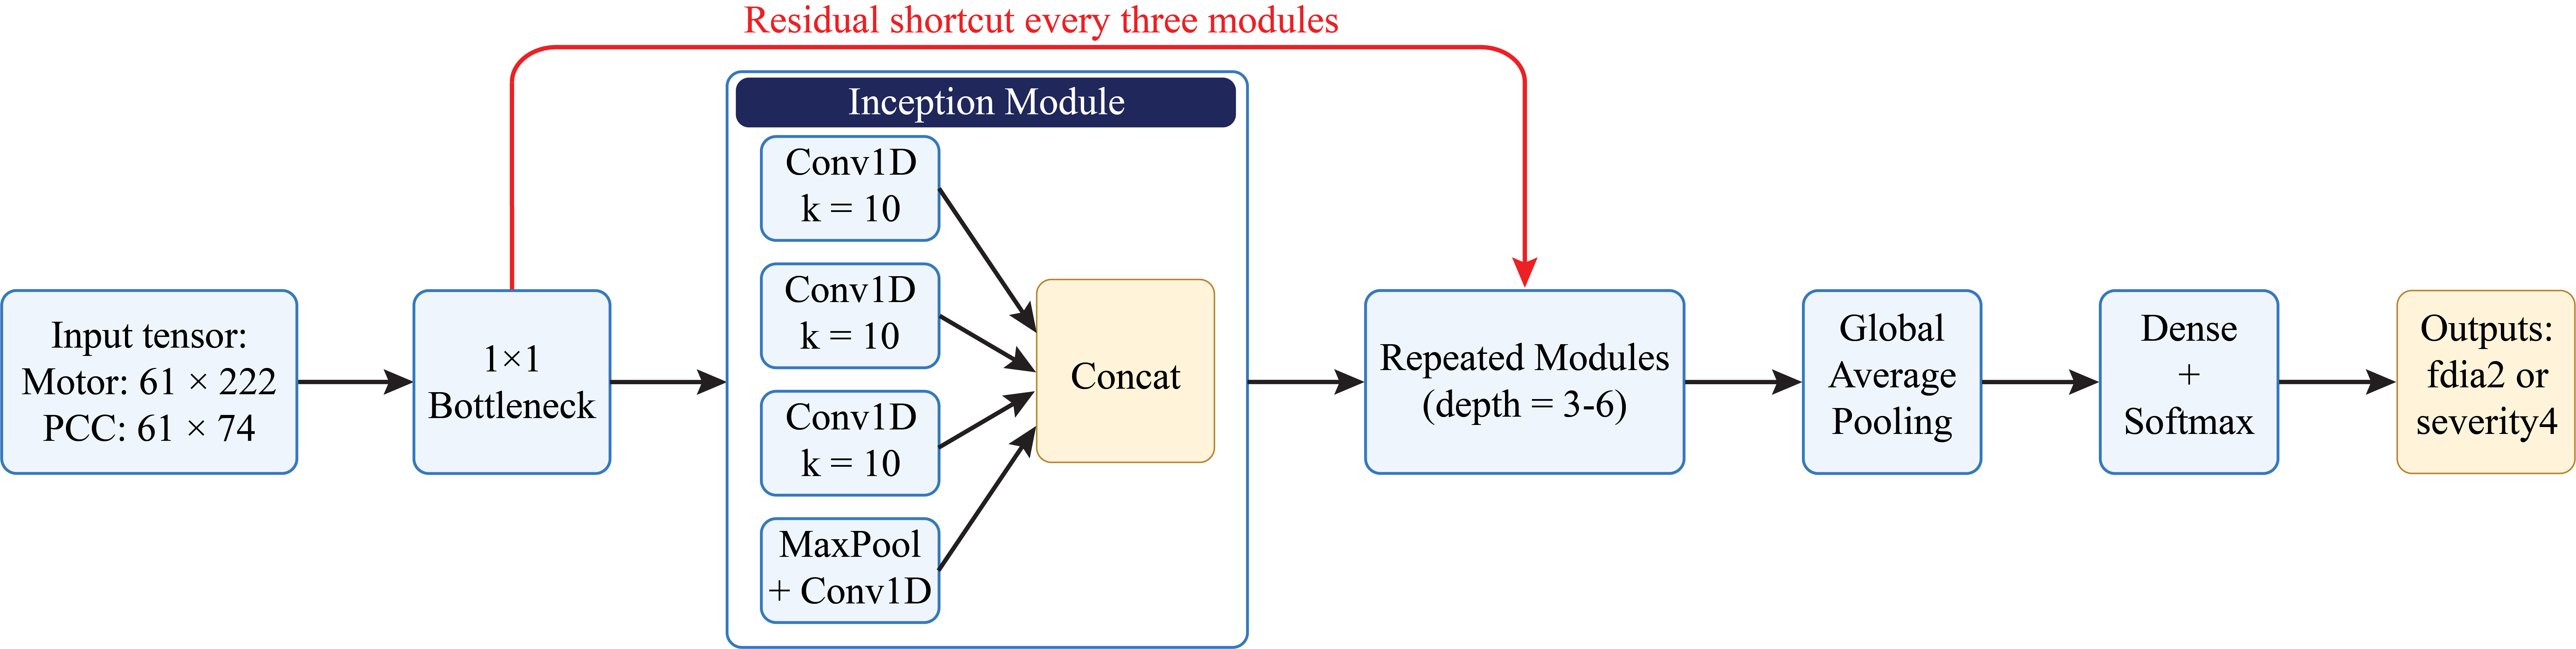
\includegraphics[width=515.52bp]{figs/inceptiontime_architecture_lfhf.png}}
\put(154.5553,83.8346){\color[rgb]{0.933333,0.960784,0.988235}\rule{31.7166bp}{8.5584bp}}
\put(170.4136,88.1138){\makebox(0,0){\color[rgb]{0,0,0}\fontsize{8bp}{9bp}\selectfont k = 39}}
\put(154.5553,58.4110){\color[rgb]{0.933333,0.960784,0.988235}\rule{31.7166bp}{8.5584bp}}
\put(170.4136,62.6902){\makebox(0,0){\color[rgb]{0,0,0}\fontsize{8bp}{9bp}\selectfont k = 19}}
\put(154.5553,32.7357){\color[rgb]{0.933333,0.960784,0.988235}\rule{31.7166bp}{8.5584bp}}
\put(170.4136,37.0149){\makebox(0,0){\color[rgb]{0,0,0}\fontsize{8bp}{9bp}\selectfont k = 9}}

\put(481.0000,37.0000){\color[rgb]{1,0.953,0.851}\rule{32.5000bp}{32.0000bp}}
\put(497.2000,53.3000){\makebox(0,0){\color[rgb]{0,0,0}\fontsize{8bp}{9bp}\selectfont \shortstack{Class\\output}}}
\end{picture}}
\endgroup
\caption{InceptionTime architecture for FDIA detection, severity assessment, and attack localization.}
\label{fig:inceptiontime_architecture}

\end{minipage}
\end{minipage}
\end{adjustbox}
\end{figure*}




\DIFaddend \subsection{Architecture of Online FDIA Detection and Attack-Severity Estimation}
\label{sec:AnomalyDetection}
\DIFaddbegin

\DIFaddend The proposed pipeline supports online monitoring from trusted motor-terminal \DIFdelbegin \DIFdel{or PCC }\DIFdelend \DIFaddbegin \DIFadd{currents or PCC voltage and }\DIFaddend current measurements. \DIFdelbegin \DIFdel{Figure}\DIFdelend \DIFaddbegin \DIFadd{Fig.}\DIFaddend ~\ref{fig:Online-algorithem} illustrates the overall architecture of the proposed monitoring pipeline. In the deployed setting, fixed-length windows of \DIFdelbegin \DIFdel{current }\DIFdelend \DIFaddbegin \DIFadd{measurement }\DIFaddend data are acquired from either the motor terminals or the PCC, passed through the LF/HF\DIFaddbegin \DIFadd{/TD }\DIFaddend feature-extraction stage, and then evaluated by the selected learning model to produce anomaly or severity decisions. The measurement, feature-extraction, and inference stages are modular, allowing the same pipeline to operate with motor-side or PCC inputs and supporting feature pruning, reduced-input models, and cross-motor adaptation. The framework provides alarms, severity indicators, and logs for supervisory systems; automatic mitigation is outside the scope. The same architecture is used for binary detection and severity classification\DIFdelbegin \DIFdel{. Binary detection is the primary PCC deployment task; severity estimates provide secondary diagnostic information. The experimental results in later sections show that motor-terminal sensing provides cleaner discriminative signatures, whereas PCC sensing offers a less intrusive sensing option for the tested setup}\DIFdelend \DIFaddbegin \DIFadd{, with separate normalization and trained models for motor-side and PCC inputs}\DIFaddend .



\DIFaddbegin \begin{figure*}[p]
\centering
\begin{adjustbox}{max width=\textwidth,max totalheight=0.87\textheight}
\begin{minipage}{\textwidth}
\centering
% Complete old block: fig:Online-algorithem
\begin{minipage}[t]{\textwidth}
\centering
\textcolor{red}{\textbf{ORIGINAL --- Figure 4 (main.tex)}}\par\smallskip

\centering
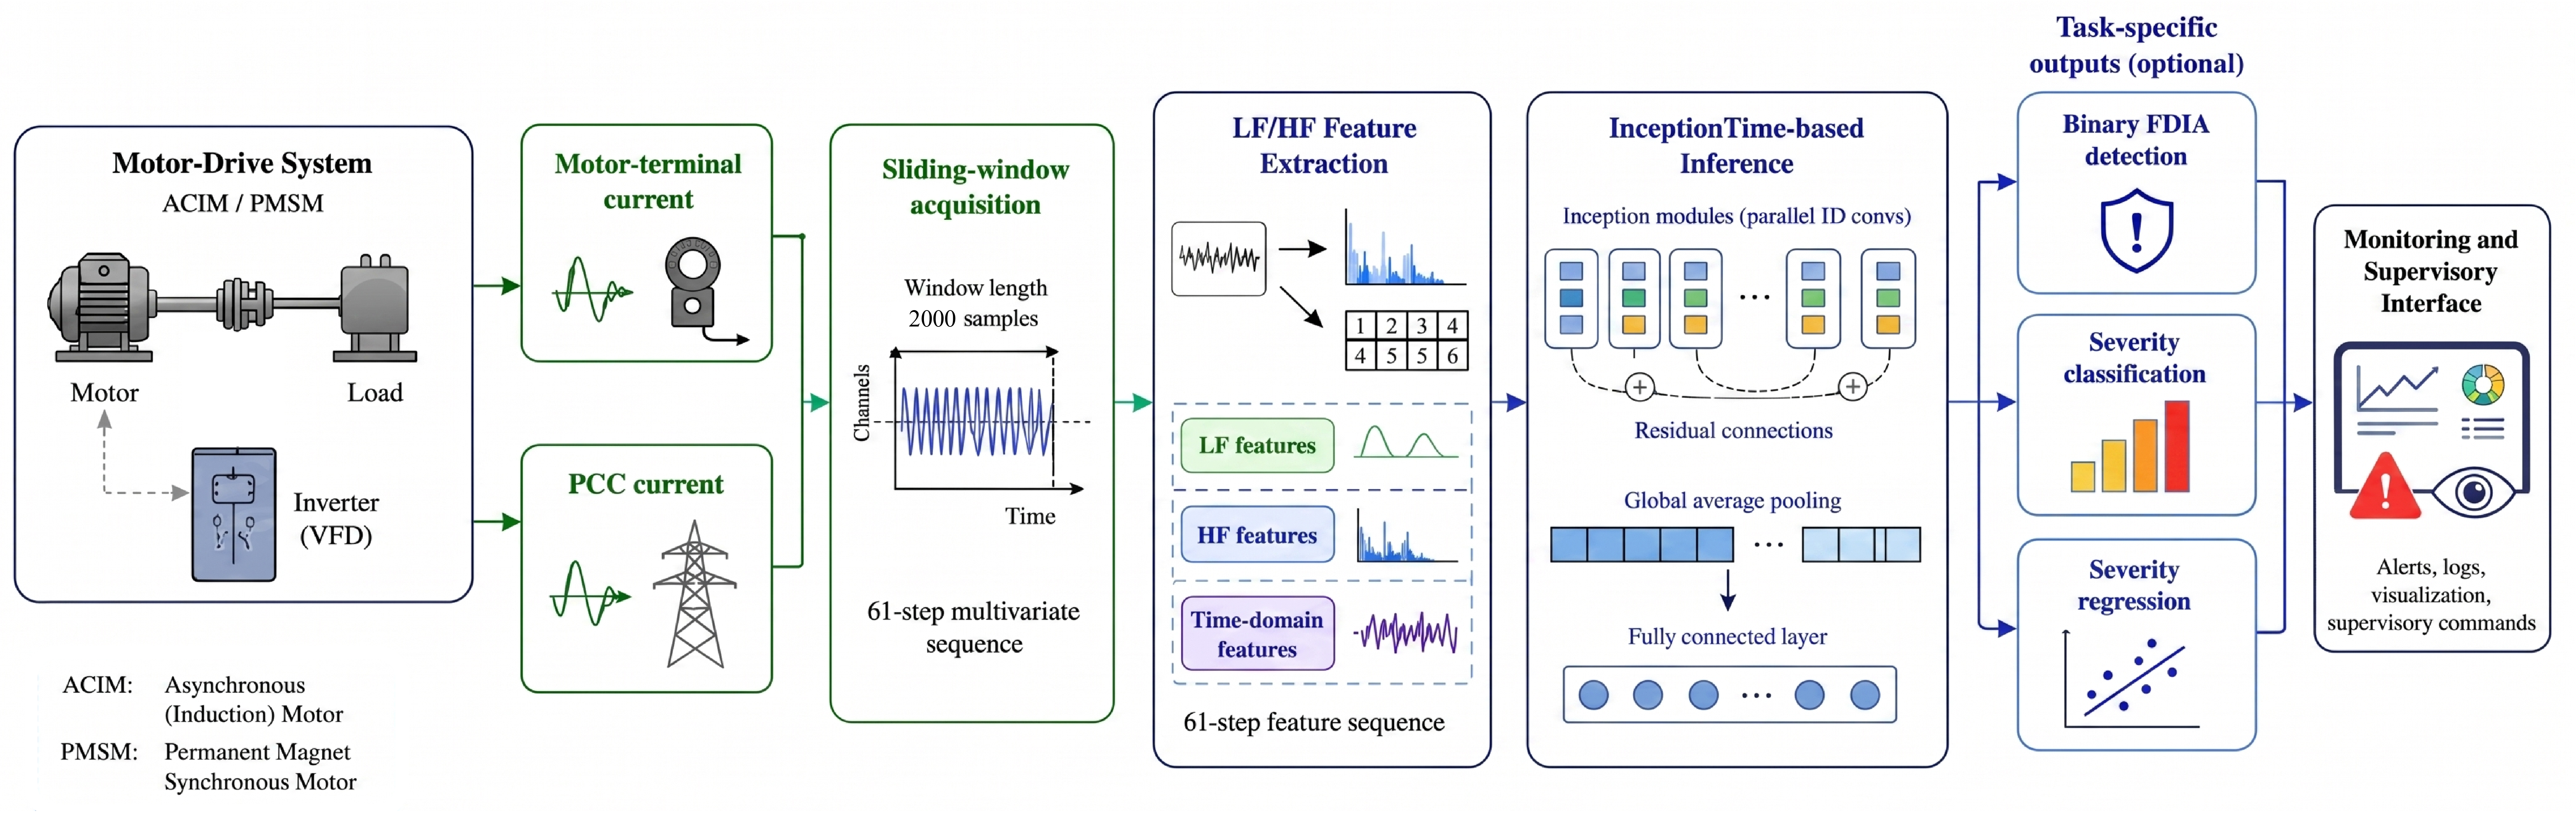
\includegraphics[width=0.99\linewidth]{figs/online_fdia_architecture.png}
\DiffOriginalCaption{Figure 4: Online FDIA detection and severity-assessment architecture for motor-side and PCC-side sensing.}


\end{minipage}\par\vspace{1em}
% Complete new block: fig:Online-algorithem
\begin{minipage}[t]{\textwidth}
\centering
\textcolor{blue}{\textbf{REVISED --- Figure 4 (main\_revised.tex)}}\par\smallskip

\centering
\begingroup
\setlength{\unitlength}{1bp}
\resizebox{\linewidth}{!}{\begin{picture}(515.5200,186.7023)
\put(0,23){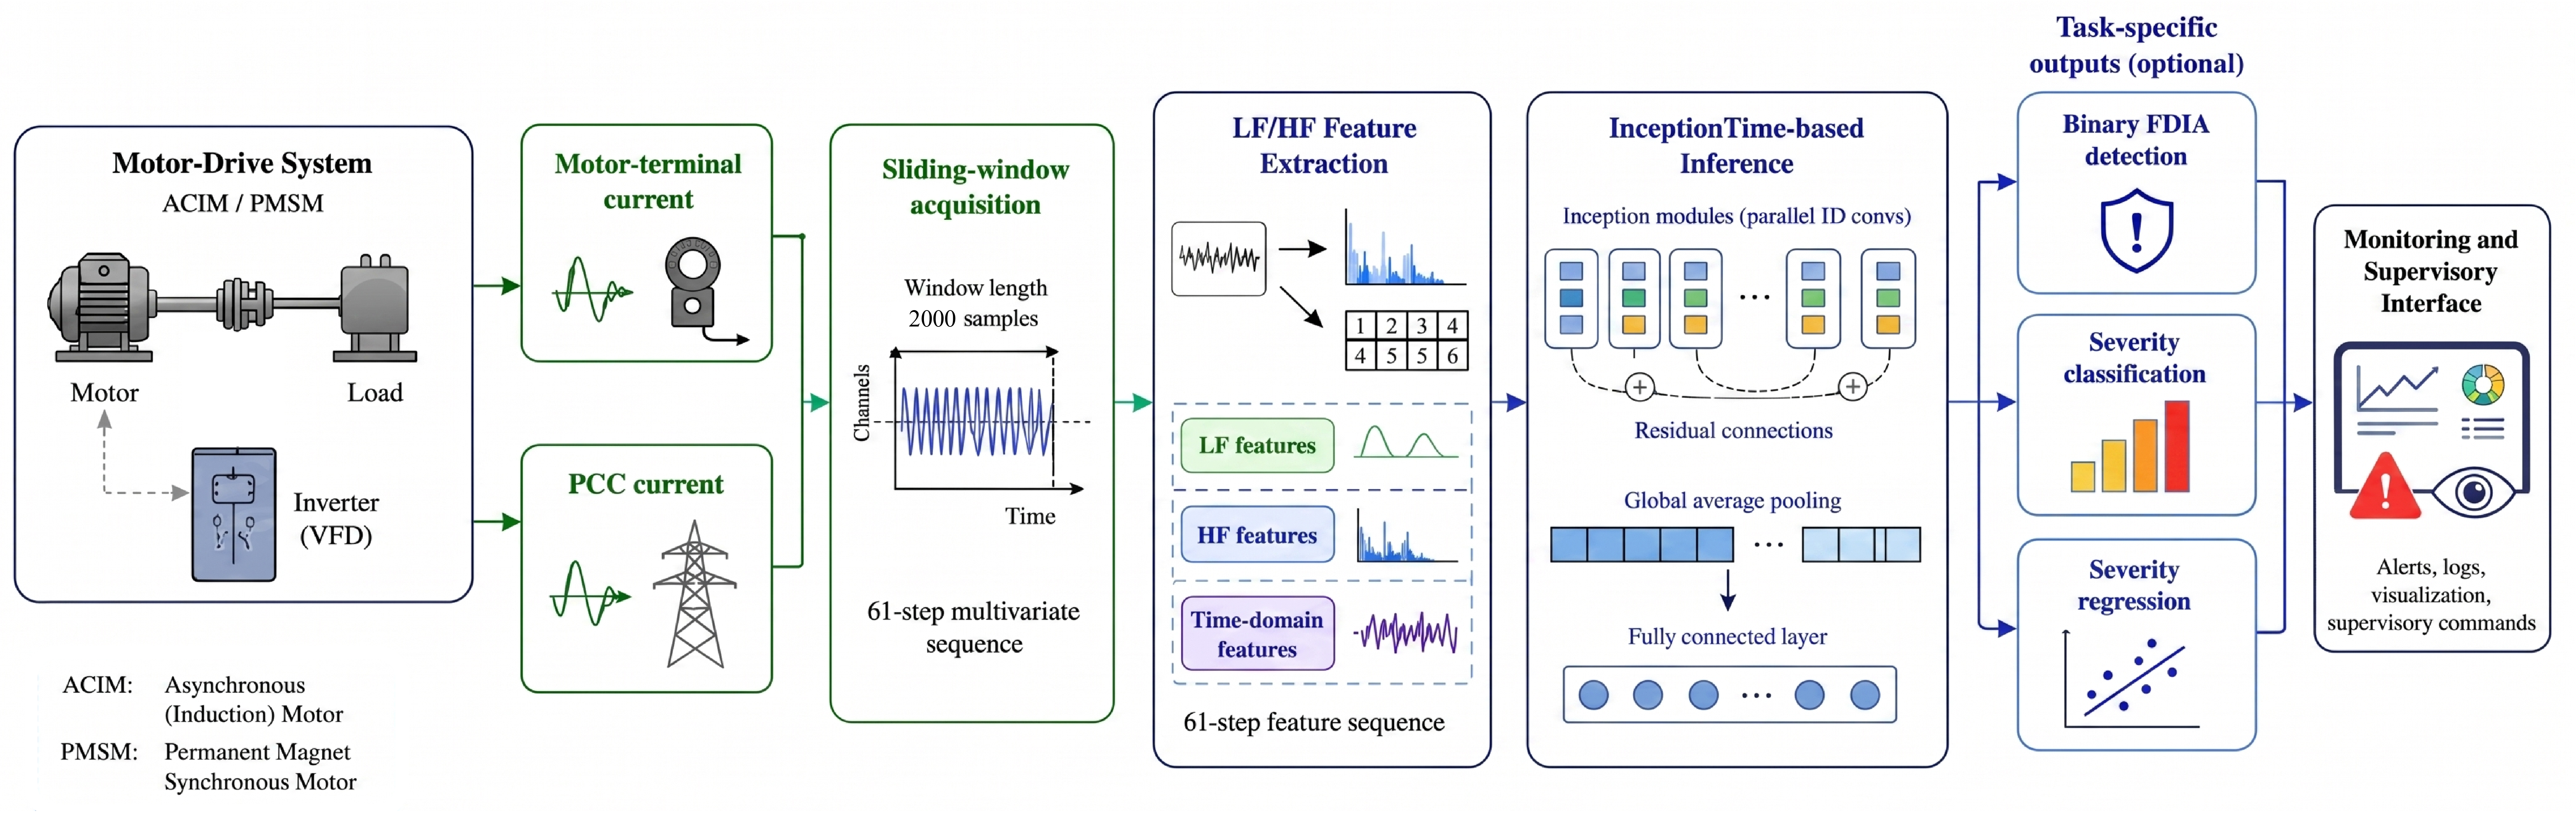
\includegraphics[width=515.52bp]{figs/online_fdia_architecture.png}}
\put(107.7356,143.6584){\color[rgb]{1,1,1}\rule{43.5473bp}{14.3480bp}}
\put(129.5093,150.8324){\makebox(0,0){\color[rgb]{0.05,0.32,0.09}\fontsize{6bp}{7bp}\selectfont \bfseries \shortstack{Motor-terminal\\currents}}}
\put(107.4839,81.7356){\color[rgb]{1,1,1}\rule{43.7991bp}{13.3411bp}}
\put(129.3834,88.4061){\makebox(0,0){\color[rgb]{0.05,0.32,0.09}\fontsize{6bp}{7bp}\selectfont \bfseries \shortstack{PCC voltage\\and current}}}
\put(169.9102,53.7948){\color[rgb]{1,1,1}\rule{50.8472bp}{16.1100bp}}
\put(195.3337,61.8498){\makebox(0,0){\color[rgb]{0,0,0}\fontsize{5.7bp}{6.7bp}\selectfont \shortstack{2,000-sample\\multichannel window}}}
\put(233.8467,36.9296){\color[rgb]{1,1,1}\rule{61.6711bp}{10.5722bp}}
\put(264.6823,42.2157){\makebox(0,0){\color[rgb]{0,0,0}\fontsize{5.7bp}{6.7bp}\selectfont \shortstack{61-step multivariate\\feature sequence}}}
\put(465.4280,58.3257){\color[rgb]{1,1,1}\rule{42.5405bp}{19.3823bp}}
\put(486.6982,68.0169){\makebox(0,0){\color[rgb]{0,0,0}\fontsize{5.7bp}{6.7bp}\selectfont \shortstack{Alerts, logs,\\visualization}}}
\put(243.4120,151.2100){\color[rgb]{1,1,1}\rule{48.3300bp}{14.3480bp}}
\put(267.5770,158.3839){\makebox(0,0){\color[rgb]{0.08,0.08,0.32}\fontsize{6bp}{7bp}\selectfont \bfseries \shortstack{LF/HF/TD Feature\\Extraction}}}
\put(155.5000,102.0000){\color[rgb]{1,1,1}\rule{9.3000bp}{9.0000bp}}
\put(160.1000,106.5000){\makebox(0,0){\color[rgb]{0.05,0.32,0.09}\fontsize{5.3bp}{6.3bp}\selectfont \bfseries OR}}
\put(257.7600,15.5000){\makebox(0,0){\color[rgb]{0,0,0}\fontsize{7bp}{8bp}\selectfont Motor-terminal currents $\longrightarrow$ motor feature tensor $\longrightarrow$ motor model}}
\put(257.7600,5.5000){\makebox(0,0){\color[rgb]{0,0,0}\fontsize{7bp}{8bp}\selectfont PCC voltage and current $\longrightarrow$ PCC feature tensor $\longrightarrow$ PCC model}}
\end{picture}}
\endgroup
\caption{Online FDIA detection and severity-assessment architecture using separate motor-terminal and PCC sensing configurations.}
\label{fig:Online-algorithem}

\end{minipage}
\end{minipage}
\end{adjustbox}
\end{figure*}




\DIFaddend \subsection{Training Details and Hyperparameters}
\label{sec:training_details}

For the InceptionTime-based models, hyperparameter selection was performed separately for \DIFaddbegin \texttt{\DIFadd{fdia2}} \DIFadd{and }\texttt{\DIFadd{severity4}} \DIFadd{in }\DIFaddend the motor and PCC streams using validation-set balanced accuracy. The search varied depth \DIFdelbegin \DIFdel{, filters, bottleneck size, dropout }\DIFdelend \DIFaddbegin \DIFadd{(3/4/6), filters (16/24/32/48), bottleneck width (8/16/32), dropout (0.20/0.35/0.50)}\DIFaddend , learning rate \DIFaddbegin \DIFadd{($5\times10^{-4}$/$10^{-3}$)}\DIFaddend , weight decay \DIFaddbegin \DIFadd{($5\times10^{-5}$/$10^{-4}$)}\DIFaddend , and batch size \DIFaddbegin \DIFadd{(64/128)}\DIFaddend . Table~\ref{tab:search_top5_combined} summarizes the top-ranked configurations for both sensing streams \DIFaddbegin \DIFadd{across all three seeds.
}

\DIFadd{The same 100 candidate configurations were evaluated for two tasks, two sensing streams, and three recording partitions, totaling 1,200 training runs.
}

\DIFadd{Training used Adam and weighted cross-entropy, assigning larger weights to less frequent classes. Each run used up to 60 epochs, with early stopping after 10 epochs without improved validation balanced accuracy. The learning rate was halved after three unimproved epochs, down to $10^{-6}$. The best checkpoint and configuration were selected independently within each recording partition using validation balanced accuracy; ties followed the fixed candidate order. Test results were not used for selection. The }\texttt{\DIFadd{fdia3}} \DIFadd{model retained the }\texttt{\DIFadd{severity4}}\DIFadd{-selected configuration for each stream and holdout and was trained from fresh weights with three outputs. Its checkpoint was selected by three-class validation balanced accuracy.
}

\DIFadd{Reported test metrics are mean $\pm$ sample standard deviation over the three holdouts. Precision, recall, and F1 are macro-averaged, and balanced accuracy is the mean class recall. The standard deviations describe variation across recording assignments and model initializations, rather than independent physical replications}\DIFaddend .




\DIFaddbegin \begin{table*}[p]
\centering
\begin{adjustbox}{max width=\textwidth,max totalheight=0.87\textheight}
\begin{minipage}{\textwidth}
\centering
% Complete old block: tab:search_top5_combined
\begin{minipage}[t]{0.48\textwidth}
\centering
\textcolor{red}{\textbf{ORIGINAL --- Table 4 (main.tex)}}\par\smallskip

\centering
\scriptsize
\DiffOriginalCaption{Table 4: Top five InceptionTime configurations ranked by validation balanced accuracy on \texttt{severity4}.}

\renewcommand{\arraystretch}{1.05}
\setlength{\tabcolsep}{2.5pt}
\begin{adjustbox}{max width=\linewidth}\begin{tabular}{c c c c c c c c c}
\hline
Rank & D & F & BN & Dr & LR & WD & BS & test BA (\%) \\
\hline
\multicolumn{9}{c}{\textit{Motor stream}} \\
\hline
1 & 3 & 32 & 16 & 0.20 & 0.0010 & $5{\times}10^{-5}$ & 128 & 98.25 \\
2 & 3 & 32 & 8  & 0.20 & 0.0010 & $10^{-4}$         & 64  & 98.08 \\
3 & 3 & 16 & 16 & 0.35 & 0.0010 & $5{\times}10^{-5}$ & 128 & 98.02 \\
4 & 3 & 32 & 8  & 0.20 & 0.0010 & $5{\times}10^{-5}$ & 128 & 97.99 \\
5 & 3 & 32 & 8  & 0.35 & 0.0010 & $10^{-4}$         & 64  & 97.96 \\
\hline
\multicolumn{9}{c}{\textit{PCC stream}} \\
\hline
1 & 6 & 32 & 32 & 0.20 & 0.0010 & $10^{-4}$         & 128 & 80.22 \\
2 & 6 & 48 & 8  & 0.20 & 0.0005 & $5{\times}10^{-5}$ & 128 & 79.95 \\
3 & 3 & 48 & 32 & 0.35 & 0.0005 & $5{\times}10^{-5}$ & 64  & 79.84 \\
4 & 4 & 32 & 32 & 0.35 & 0.0005 & $10^{-4}$         & 64  & 79.56 \\
5 & 4 & 48 & 32 & 0.50 & 0.0010 & $10^{-4}$         & 128 & 79.40 \\
\hline
\end{tabular}\end{adjustbox}
\vspace{1mm}
\begin{flushleft}
\scriptsize D: depth; F: filters; BN: bottleneck; Dr: dropout; LR: learning rate; WD: weight decay; BS: batch size; test BA: test balanced accuracy.
\end{flushleft}

\end{minipage}\hfill%
% Complete new block: tab:search_top5_combined
\begin{minipage}[t]{0.48\textwidth}
\centering
\textcolor{blue}{\textbf{REVISED --- Table 4 (main\_revised.tex)}}\par\smallskip

\centering
\footnotesize
\caption{Top five \texttt{severity4} configurations
ranked by mean validation balanced accuracy
across three seeds (\%).}
\label{tab:search_top5_combined}
\renewcommand{\arraystretch}{1.10}
\setlength{\tabcolsep}{3pt}

\begin{tabular}{@{}cccccccc@{}}
\hline
Rank & D & F & BN & Dr & WD & BS &
Mean $\pm$ SD \\
\hline
\multicolumn{8}{c}{\textit{Motor stream}} \\
\hline
1 & 6 & 48 & 32 & 0.35 & 5e-5 &
64 & 93.09 $\pm$ 2.45 \\
2 & 6 & 24 & 16 & 0.20 & 1e-4 &
128 & 92.59 $\pm$ 0.99 \\
3 & 3 & 16 & 16 & 0.50 & 5e-5 &
64 & 92.19 $\pm$ 2.24 \\
4 & 3 & 24 & 16 & 0.50 & 1e-4 &
128 & 92.13 $\pm$ 2.97 \\
5 & 3 & 16 & 16 & 0.50 & 1e-4 &
64 & 92.02 $\pm$ 1.02 \\
\hline
\multicolumn{8}{c}{\textit{PCC stream}} \\
\hline
1 & 6 & 32 & 32 & 0.50 & 1e-4 &
64 & 55.98 $\pm$ 3.31 \\
2 & 4 & 48 & 32 & 0.20 & 5e-5 &
64 & 55.82 $\pm$ 4.09 \\
3 & 6 & 48 & 32 & 0.35 & 5e-5 &
64 & 55.38 $\pm$ 3.17 \\
4 & 6 & 24 & 16 & 0.50 & 5e-5 &
128 & 55.31 $\pm$ 4.86 \\
5 & 4 & 32 & 32 & 0.50 & 5e-5 &
64 & 55.19 $\pm$ 4.42 \\
\hline
\end{tabular}

\par\smallskip
\begin{minipage}{\columnwidth}
\scriptsize
D: depth; F: filters; BN: bottleneck;
Dr: dropout; WD: weight decay;
BS: batch size. Learning rate is fixed
at 0.001. SD denotes sample standard
deviation across three seeds.
The ranking summarizes validation performance;
test models are selected independently
within each seed.
\end{minipage}

\end{minipage}
\end{minipage}
\end{adjustbox}
\end{table*}































\DIFaddend \subsection{Domain Adaptation Strategy: Source-Only vs Few-Shot Fine-Tuning}
\label{sec:domain_adaptation}
\DIFaddbegin

\DIFaddend Few-shot adaptation was evaluated by training on \DIFdelbegin \DIFdel{one motor type }\DIFdelend \DIFaddbegin \DIFadd{recordings targeting one motor }\DIFaddend and testing on \DIFaddbegin \DIFadd{recordings targeting }\DIFaddend the other. Two transfer directions were considered: ACIM $\rightarrow$ PMSM and PMSM $\rightarrow$ ACIM. For each direction, the detector was first trained using labeled \DIFdelbegin \DIFdel{data from the source motor only }\DIFdelend \DIFaddbegin \DIFadd{source recordings }\DIFaddend and then evaluated directly on the target \DIFdelbegin \DIFdel{motor}\DIFdelend \DIFaddbegin \DIFadd{recordings}\DIFaddend . This \emph{source-only} setting quantifies cross-motor domain shift. \DIFaddbegin \DIFadd{Six source recordings were used for training and three for validation, with the 100-candidate search selected by source validation balanced accuracy.
}\DIFaddend

For adaptation, the source-trained model was fine-tuned using a small labeled subset of \DIFaddbegin \DIFadd{complete }\DIFaddend target-domain \DIFdelbegin \DIFdel{samples }\DIFdelend \DIFaddbegin \DIFadd{episode groups }\DIFaddend before testing on \DIFdelbegin \DIFdel{held-out target data. The }\DIFdelend \DIFaddbegin \DIFadd{separate target recordings. The nominal }\DIFaddend target adaptation ratios considered in this work were 1\%, 5\%, 10\%, and 20\% of the available target-domain adaptation pool \DIFaddbegin \DIFadd{(Table~\ref{tab:evaluation_protocols}); the 1\% budget selects two of 180 groups (1.11\%). Fine-tuning used 20 epochs at 0.2 times the source learning rate, with source normalization fixed}\DIFaddend .
The domain-adaptation strategy was implemented as supervised fine-tuning rather than unsupervised feature alignment. Accordingly, all reported adaptation gains reflect the benefit of limited labeled target-domain data under a practical transfer-learning setting. To ensure reliable comparison, all cross-domain experiments were repeated over three random seeds\DIFdelbegin \DIFdel{, and the results were reported using both accuracy and balanced accuracy}\DIFdelend .



\DIFdelbegin \DIFdel{This protocol is particularly important in the present study because ACIM and PMSM signals exhibit substantial domain differences despite being collected under the same FDIA framework. This tests whether the LF/HF-Inception representation can be adapted with limited target-domain labels.
}\DIFdelend \section{Experimental Results}
\label{sec:results}
\DIFdelbegin \subsection{\DIFdel{In-Domain Baselines: Motor vs PCC}}
%DIFAUXCMD
\addtocounter{subsection}{-1}%DIFAUXCMD
%DIFDELCMD < \label{sec:in_domain}
%DIFDELCMD < %%%
\DIFdelend

Table~\ref{tab:all_tasks_in_domain} reports mixed-domain in-domain performance with ACIM and PMSM \DIFdelbegin \DIFdel{samples }\DIFdelend \DIFaddbegin \DIFadd{recordings }\DIFaddend in all splits \DIFdelbegin \DIFdel{. }\DIFdelend \DIFaddbegin \DIFadd{and no shared recordings or episodes between them.
}\subsection{\DIFadd{In-Domain Baselines: Motor vs PCC}}
\label{sec:in_domain}

\DIFaddend The results show that motor-side sensing provides more discriminative attack signatures than PCC sensing for both \DIFdelbegin \DIFdel{(}\DIFdelend \texttt{fdia2} \DIFdelbegin \DIFdel{) and (}\DIFdelend \DIFaddbegin \DIFadd{and }\DIFaddend \texttt{severity4}\DIFdelbegin \DIFdel{)}\DIFdelend . In addition, \DIFdelbegin \DIFdel{(}\DIFdelend \texttt{severity4} \DIFdelbegin \DIFdel{) }\DIFdelend is substantially more challenging than binary attack detection, especially at PCC. \DIFaddbegin \DIFadd{The }\texttt{\DIFadd{fdia3}} \DIFadd{rows report joint detection and localization, including the normal class. Fig.~\ref{fig:main_confusion_matrices} shows the }\texttt{\DIFadd{fdia2}} \DIFadd{and }\texttt{\DIFadd{fdia3}} \DIFadd{confusion matrices; Fig.~\ref{fig:severity_detection_decisions}(a), (b) shows the }\texttt{\DIFadd{severity4}} \DIFadd{matrices. Row percentages are pooled over the three holdouts.
}\DIFaddend



\DIFaddbegin \DIFadd{Exact-severity recall counts attacks assigned to the correct bias class. Severity-conditioned attack recall also counts attacks assigned to another nonzero bias class. Fig.~\ref{fig:severity_detection_decisions}(c), (d) presents this second view of the PCC severity model: it detects 88.1\% of high-bias attacks as some attack level, compared with 70.8\% assigned to the exact high-bias class. }\DIFaddend Thus, \DIFdelbegin \DIFdel{PCC-side severity estimates should be treated as coarse diagnostics, whereas motor-side measurements support finer severity discrimination. Overall, PCC monitoring is more challenging than motor-side monitoring, and severity assessment is harder than binary detection . These baseline findings motivate the subsequent cross-domain analysis, where the additional challenge of motor-type shift is introduced}\DIFdelend \DIFaddbegin \DIFadd{an incorrect severity estimate can still provide an attack indication. The same model labels 37.3\% of normal windows as attacks, so this detection benefit must be considered together with false alarms. These decisions come from the four-class model; the separately trained binary detector in Fig.~\ref{fig:main_confusion_matrices}(b) has fewer false alarms}\DIFaddend .



\DIFaddbegin \begin{table*}[p]
\centering
\begin{adjustbox}{max width=\textwidth,max totalheight=0.87\textheight}
\begin{minipage}{\textwidth}
\centering
% Complete old block: tab:all_tasks_in_domain
\begin{minipage}[t]{0.48\textwidth}
\centering
\textcolor{red}{\textbf{ORIGINAL --- Table 5 (main.tex)}}\par\smallskip

\centering
\DiffOriginalCaption{Table 5: In-domain performance under the mixed ACIM/PMSM split.}

\renewcommand{\arraystretch}{1.15}
\setlength{\tabcolsep}{4pt}
\begin{adjustbox}{max width=\linewidth}\begin{tabular}{l c c c c c}
\hline
Task & Accuracy & Bal. Acc. & Precision & Recall & F1 \\
     & (\%)    & Accuracy (\%)      & (\%)   & (\%)   & (\%) \\
\hline
\multicolumn{6}{c}{\textit{PCC stream}} \\
\hline
\texttt{fdia2}      & 89.44 & 88.99 & 89.71 & 88.99 & 89.25 \\
\texttt{severity4}  & 84.17 & 80.22 & 80.50 & 80.22 & 80.32 \\
Motor type          & 100.00 & 100.00 & 100.00 & 100.00 & 100.00 \\
\hline
\multicolumn{6}{c}{\textit{Motor stream}} \\
\hline
\texttt{fdia2}      & 98.89 & 98.85 & 98.91 & 98.85 & 98.88 \\
\texttt{severity4}  & 98.68 & 98.25 & 98.22 & 98.25 & 98.24 \\
Motor type          & 100.00 & 100.00 & 100.00 & 100.00 & 100.00 \\
\hline
\end{tabular}\end{adjustbox}
\vspace{1mm}
\begin{flushleft}
\scriptsize Precision, recall, and F1 are reported as macro-averaged values in paper.
\end{flushleft}

\end{minipage}\hfill%
% Complete new block: tab:all_tasks_in_domain
\begin{minipage}[t]{0.48\textwidth}
\centering
\textcolor{blue}{\textbf{REVISED --- Table 5 (main\_revised.tex)}}\par\smallskip

\centering
\footnotesize
\caption{In-domain performance on held-out ACIM/PMSM recordings (\%).}
\label{tab:all_tasks_in_domain}
\renewcommand{\arraystretch}{1.15}
\setlength{\tabcolsep}{1.7pt}
\begin{tabular}{@{}lccccc@{}}
\hline
Task & Acc. & BA & Prec. & Recall & F1 \\\hline
\hline\multicolumn{6}{c}{\textit{PCC stream}} \\\hline
\texttt{fdia2} & \shortstack{80.78\\($\pm$2.95)} & \shortstack{80.29\\($\pm$3.03)} & \shortstack{81.04\\($\pm$3.14)} & \shortstack{80.29\\($\pm$3.03)} & \shortstack{80.42\\($\pm$2.96)} \\
\texttt{severity4} & \shortstack{61.00\\($\pm$1.32)} & \shortstack{55.62\\($\pm$2.94)} & \shortstack{52.93\\($\pm$2.36)} & \shortstack{55.62\\($\pm$2.94)} & \shortstack{52.96\\($\pm$2.15)} \\
\texttt{fdia3} & \shortstack{74.32\\($\pm$4.16)} & \shortstack{77.84\\($\pm$4.63)} & \shortstack{76.16\\($\pm$4.56)} & \shortstack{77.84\\($\pm$4.63)} & \shortstack{75.52\\($\pm$4.14)} \\
\hline\multicolumn{6}{c}{\textit{MOTOR stream}} \\\hline
\texttt{fdia2} & \shortstack{87.41\\($\pm$11.13)} & \shortstack{88.26\\($\pm$9.99)} & \shortstack{89.90\\($\pm$7.84)} & \shortstack{88.26\\($\pm$9.99)} & \shortstack{87.23\\($\pm$11.39)} \\
\texttt{severity4} & \shortstack{87.64\\($\pm$8.87)} & \shortstack{90.81\\($\pm$4.29)} & \shortstack{86.09\\($\pm$9.44)} & \shortstack{90.81\\($\pm$4.29)} & \shortstack{86.06\\($\pm$8.95)} \\
\texttt{fdia3} & \shortstack{85.64\\($\pm$9.60)} & \shortstack{89.55\\($\pm$4.47)} & \shortstack{87.95\\($\pm$8.29)} & \shortstack{89.55\\($\pm$4.47)} & \shortstack{86.70\\($\pm$8.18)} \\
\hline\end{tabular}
\par\smallskip\begin{minipage}{\columnwidth}\scriptsize Cells show mean above ($\pm$ sample SD), over three holdouts; this is not a range or confidence interval. BA: balanced accuracy. Precision, recall, and F1 are macro-averaged.\end{minipage}

\end{minipage}
\end{minipage}
\end{adjustbox}
\end{table*}






\begin{figure*}[p]
\centering
\begin{adjustbox}{max width=\textwidth,max totalheight=0.87\textheight}
\begin{minipage}{\textwidth}
\centering
% Complete old block: fig:main_confusion_matrices
\begin{minipage}[t]{\textwidth}
\centering
\textcolor{red}{\textbf{ORIGINAL --- Figure 5 (main.tex)}}\par\smallskip

    \centering

    \begin{minipage}{0.48\textwidth}
        \centering
        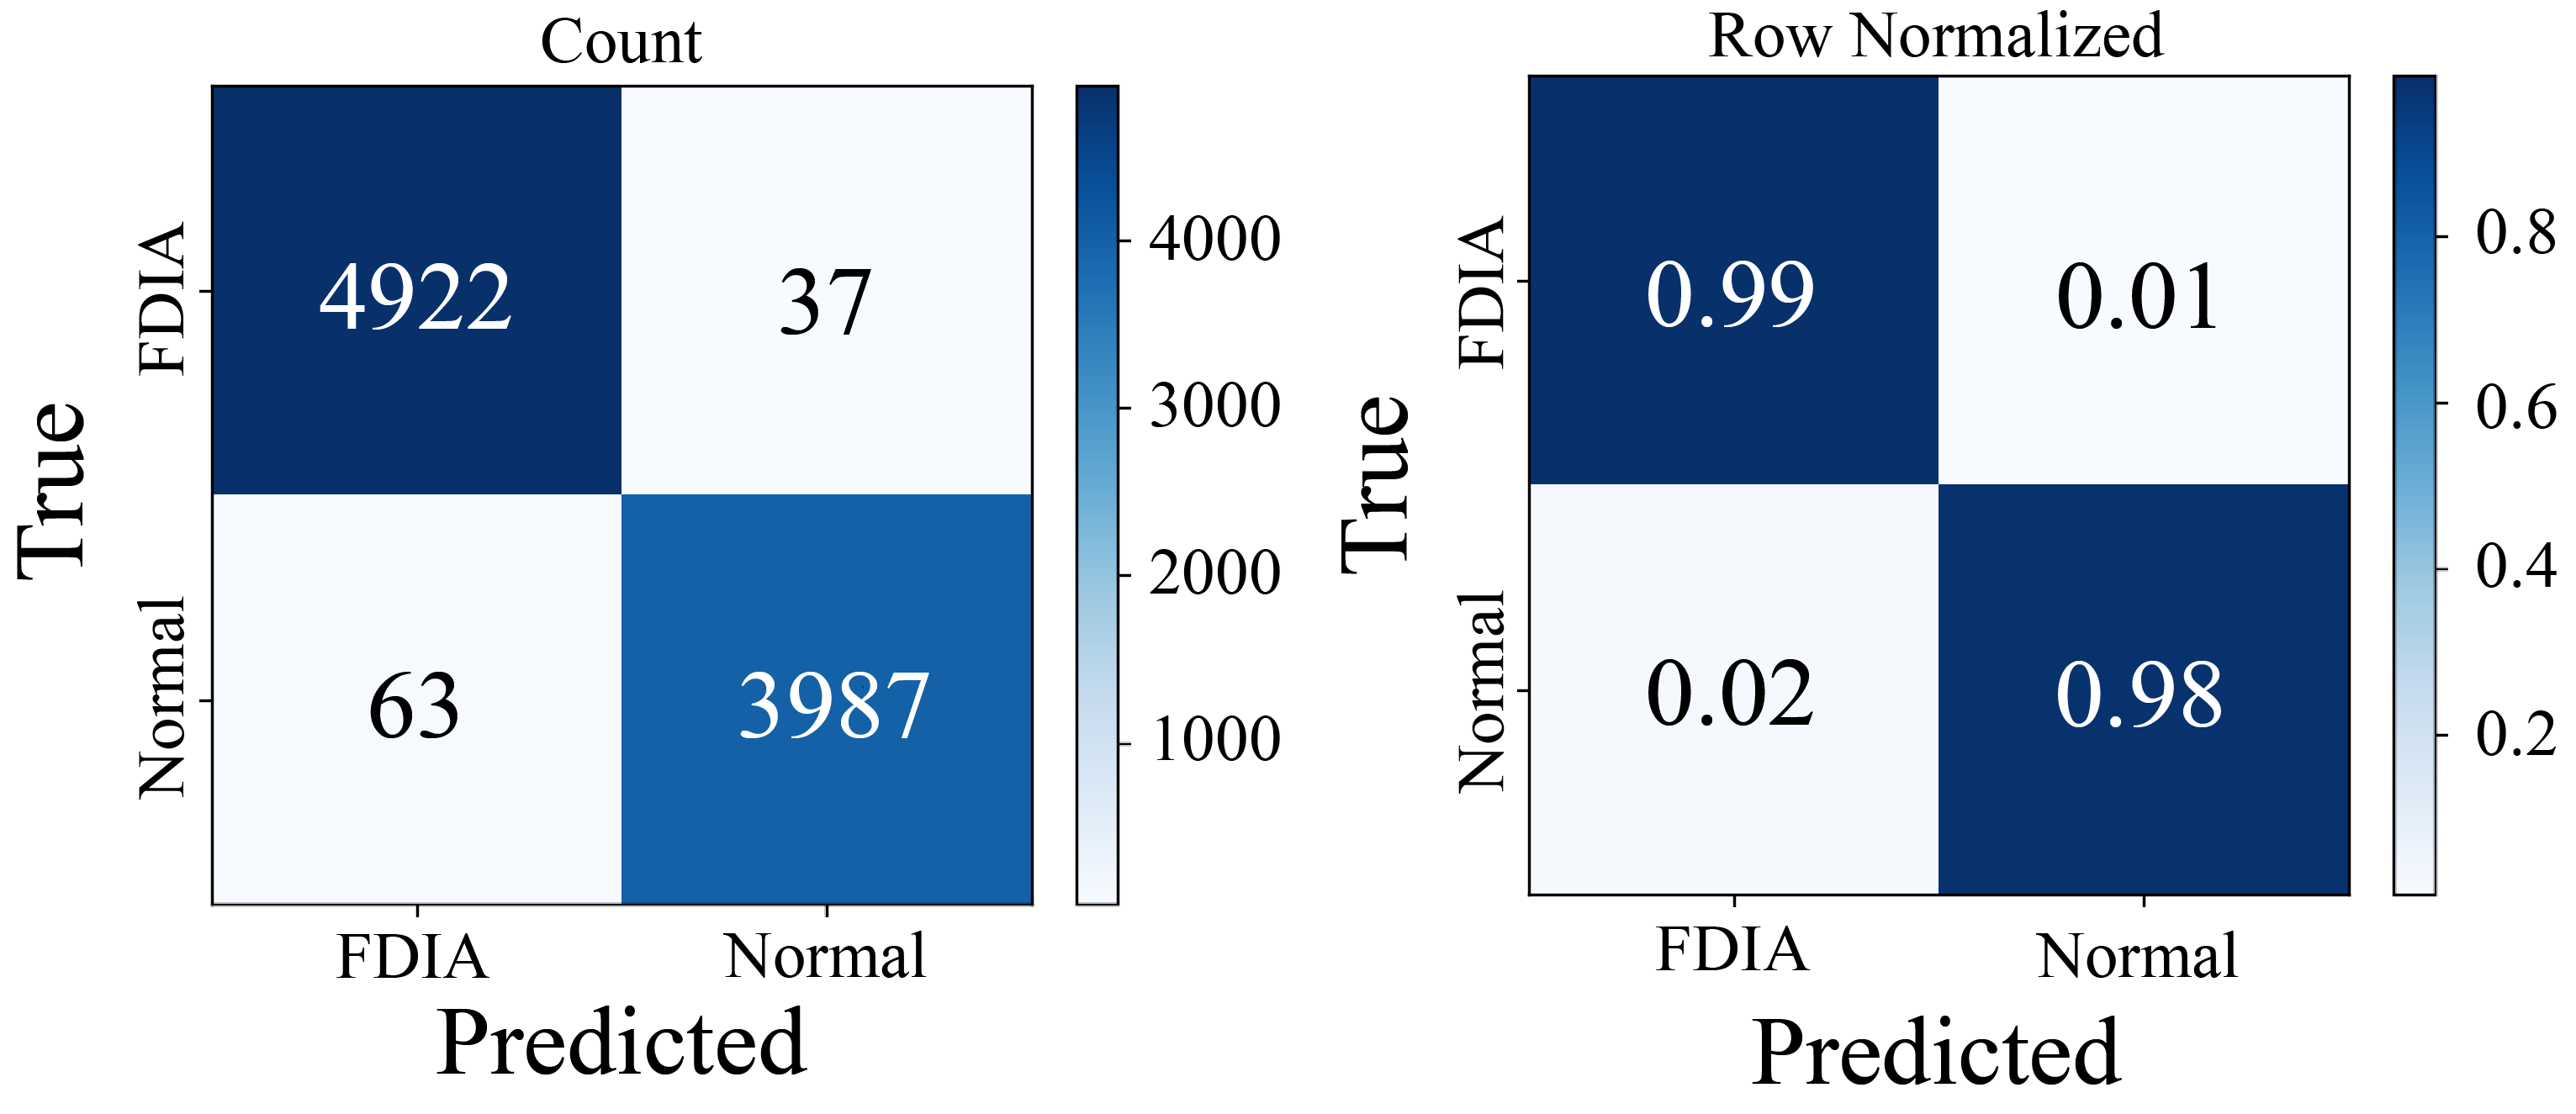
\includegraphics[width=\linewidth]{figs/anomaly2_motor_confusion_revised.png}
        \vspace{-1mm}
        \centerline{(a) \texttt{fdia2}, motor stream}
    \end{minipage}
    \hfill
    \begin{minipage}{0.48\textwidth}
        \centering
        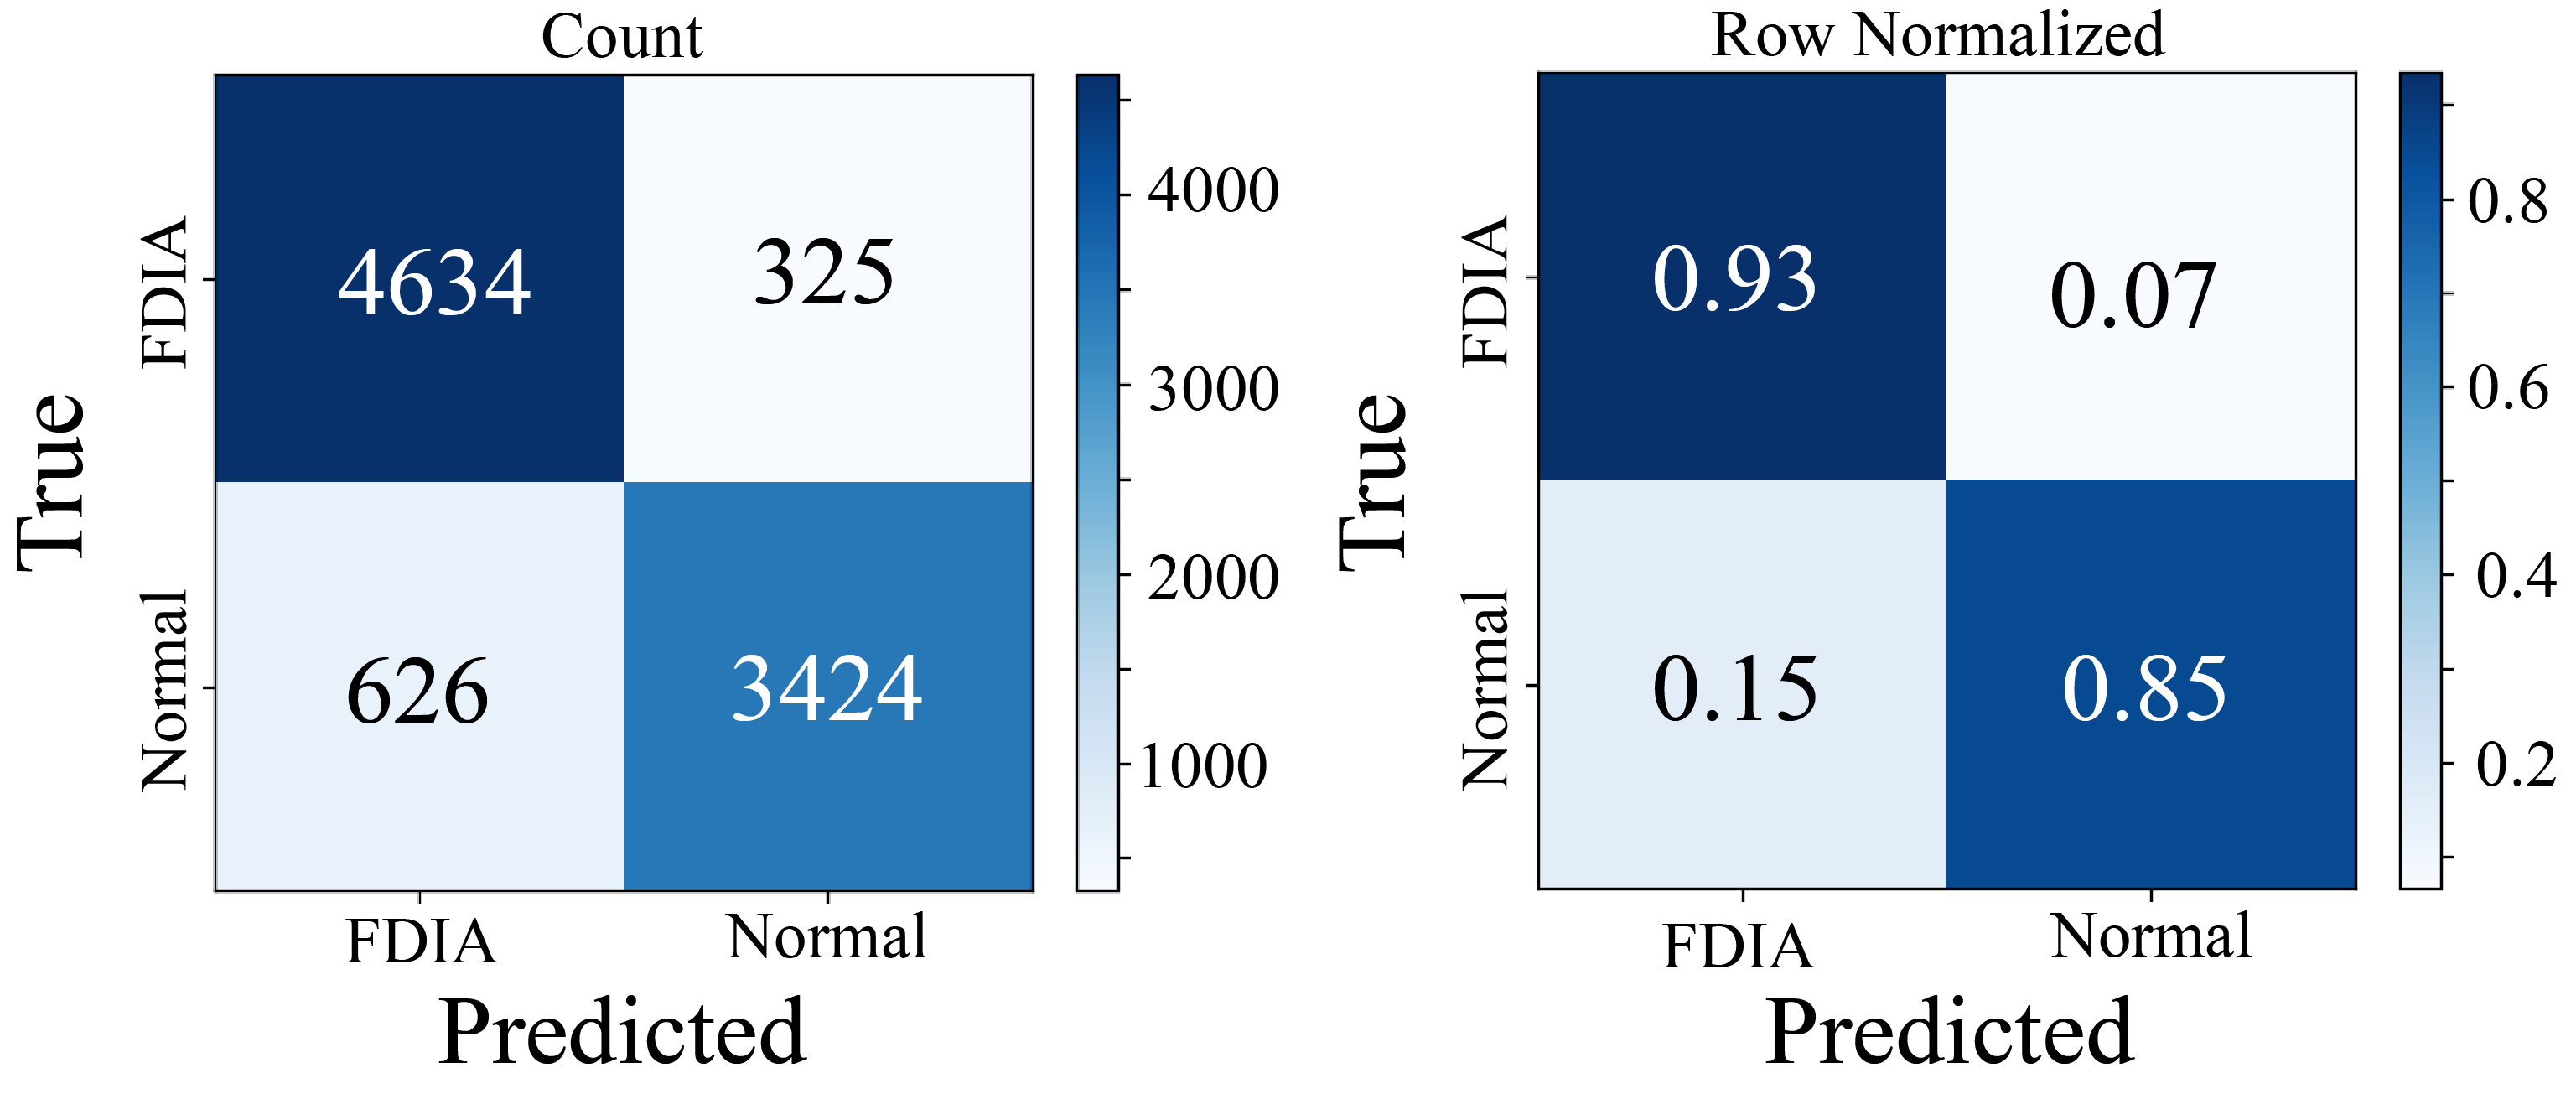
\includegraphics[width=\linewidth]{figs/anomaly2_pcc_confusion_revised.png}
        \vspace{-1mm}
        \centerline{(b) \texttt{fdia2}, PCC stream}
    \end{minipage}

    \vspace{2mm}

    \begin{minipage}{0.48\textwidth}
        \centering
        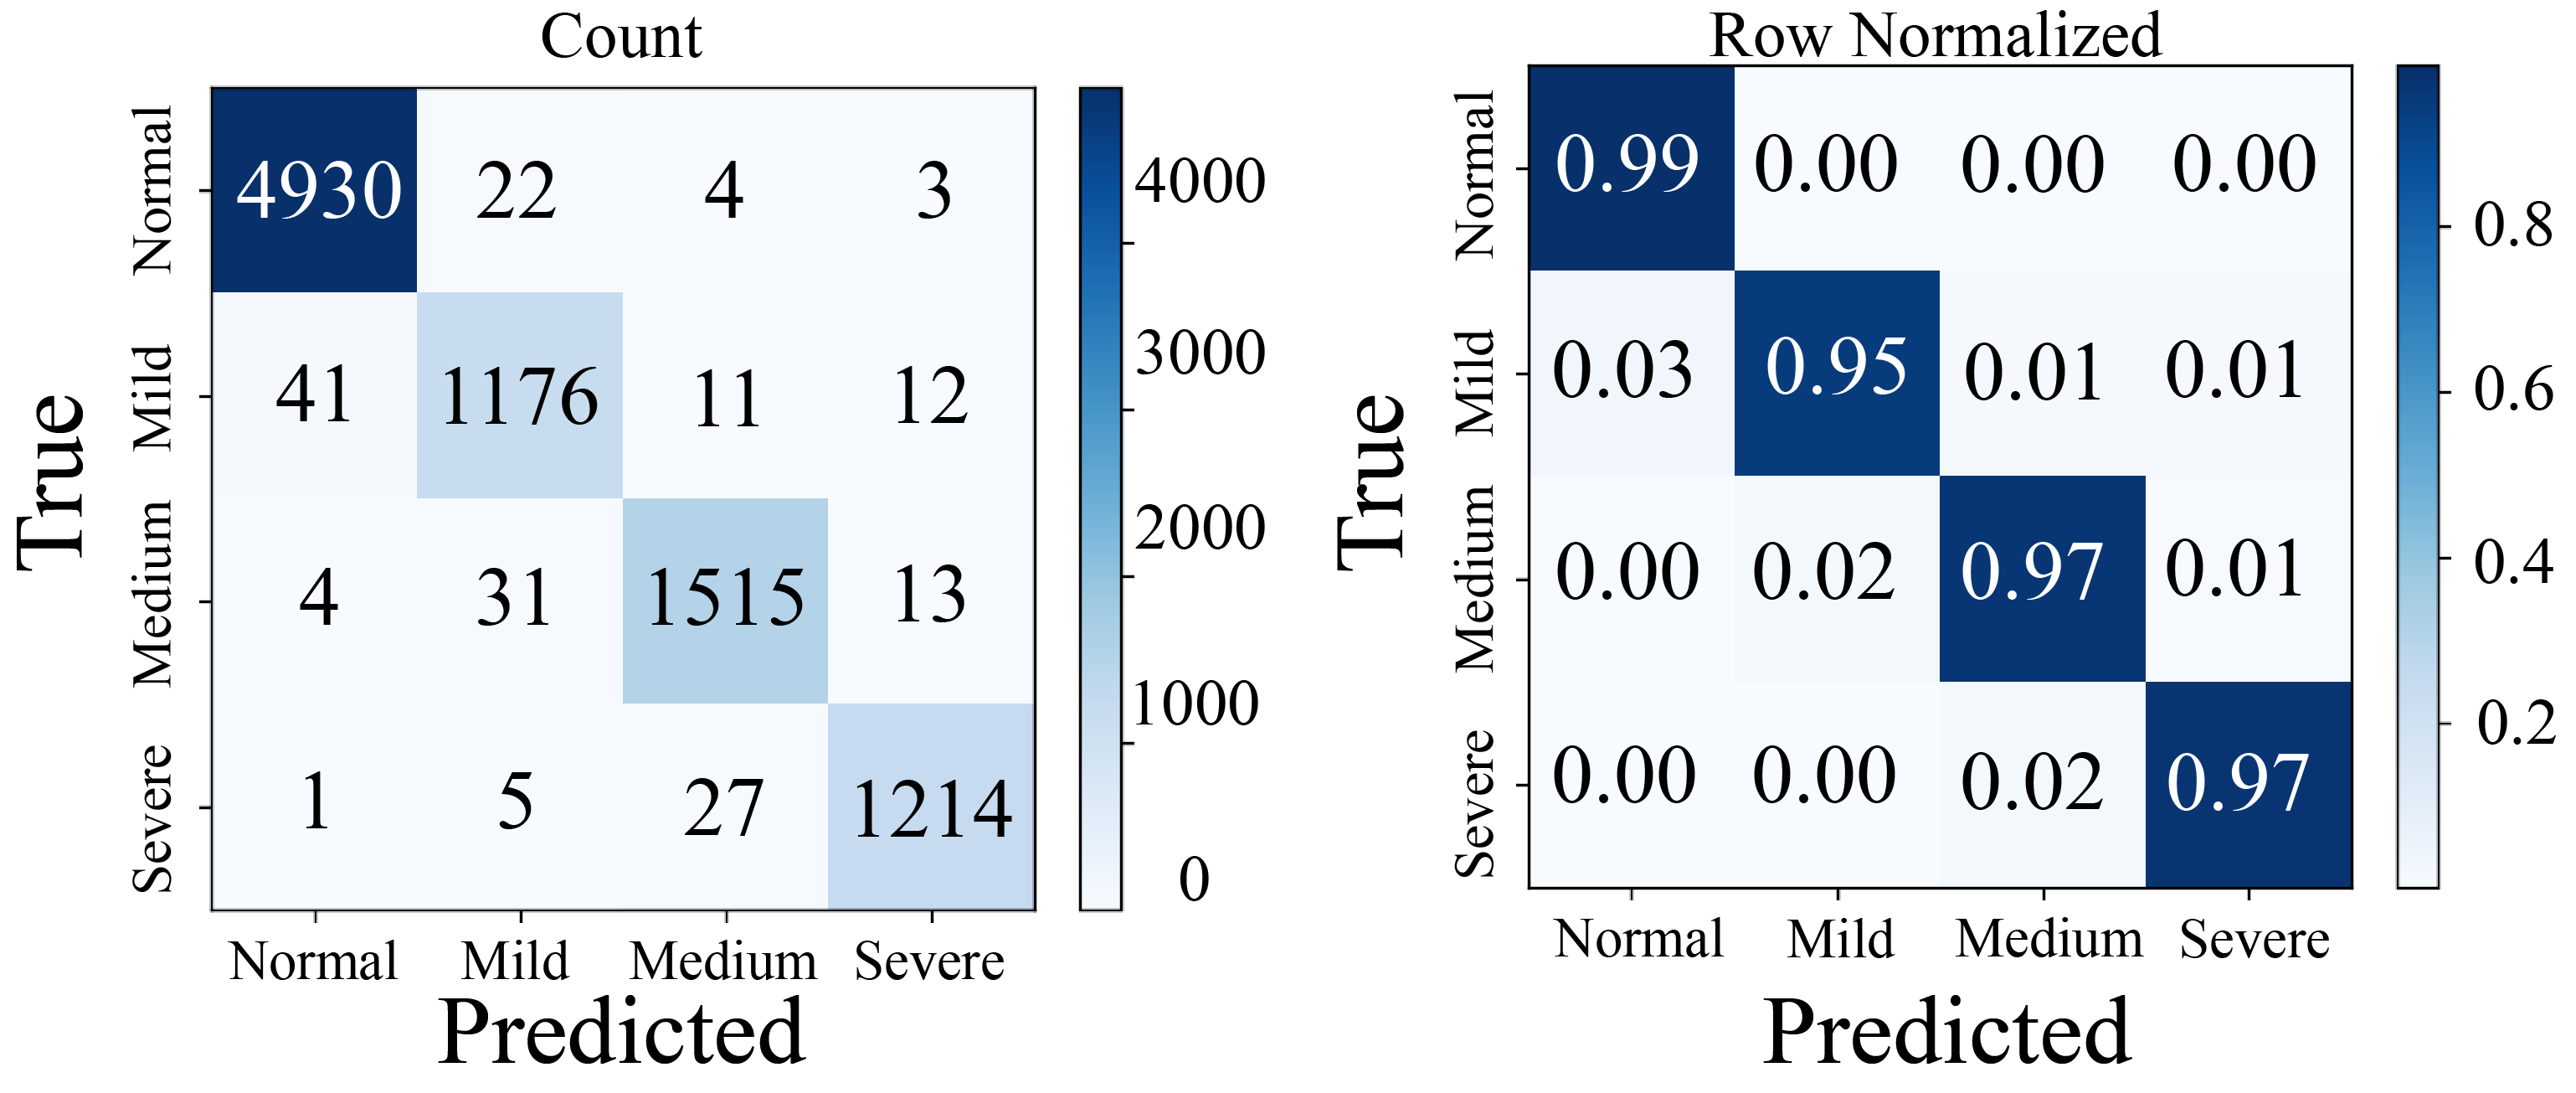
\includegraphics[width=\linewidth]{figs/severity4_motor_confusion_revised.png}
        \vspace{-1mm}
        \centerline{(c) \texttt{severity4}, motor stream}
    \end{minipage}
    \hfill
    \begin{minipage}{0.48\textwidth}
        \centering
        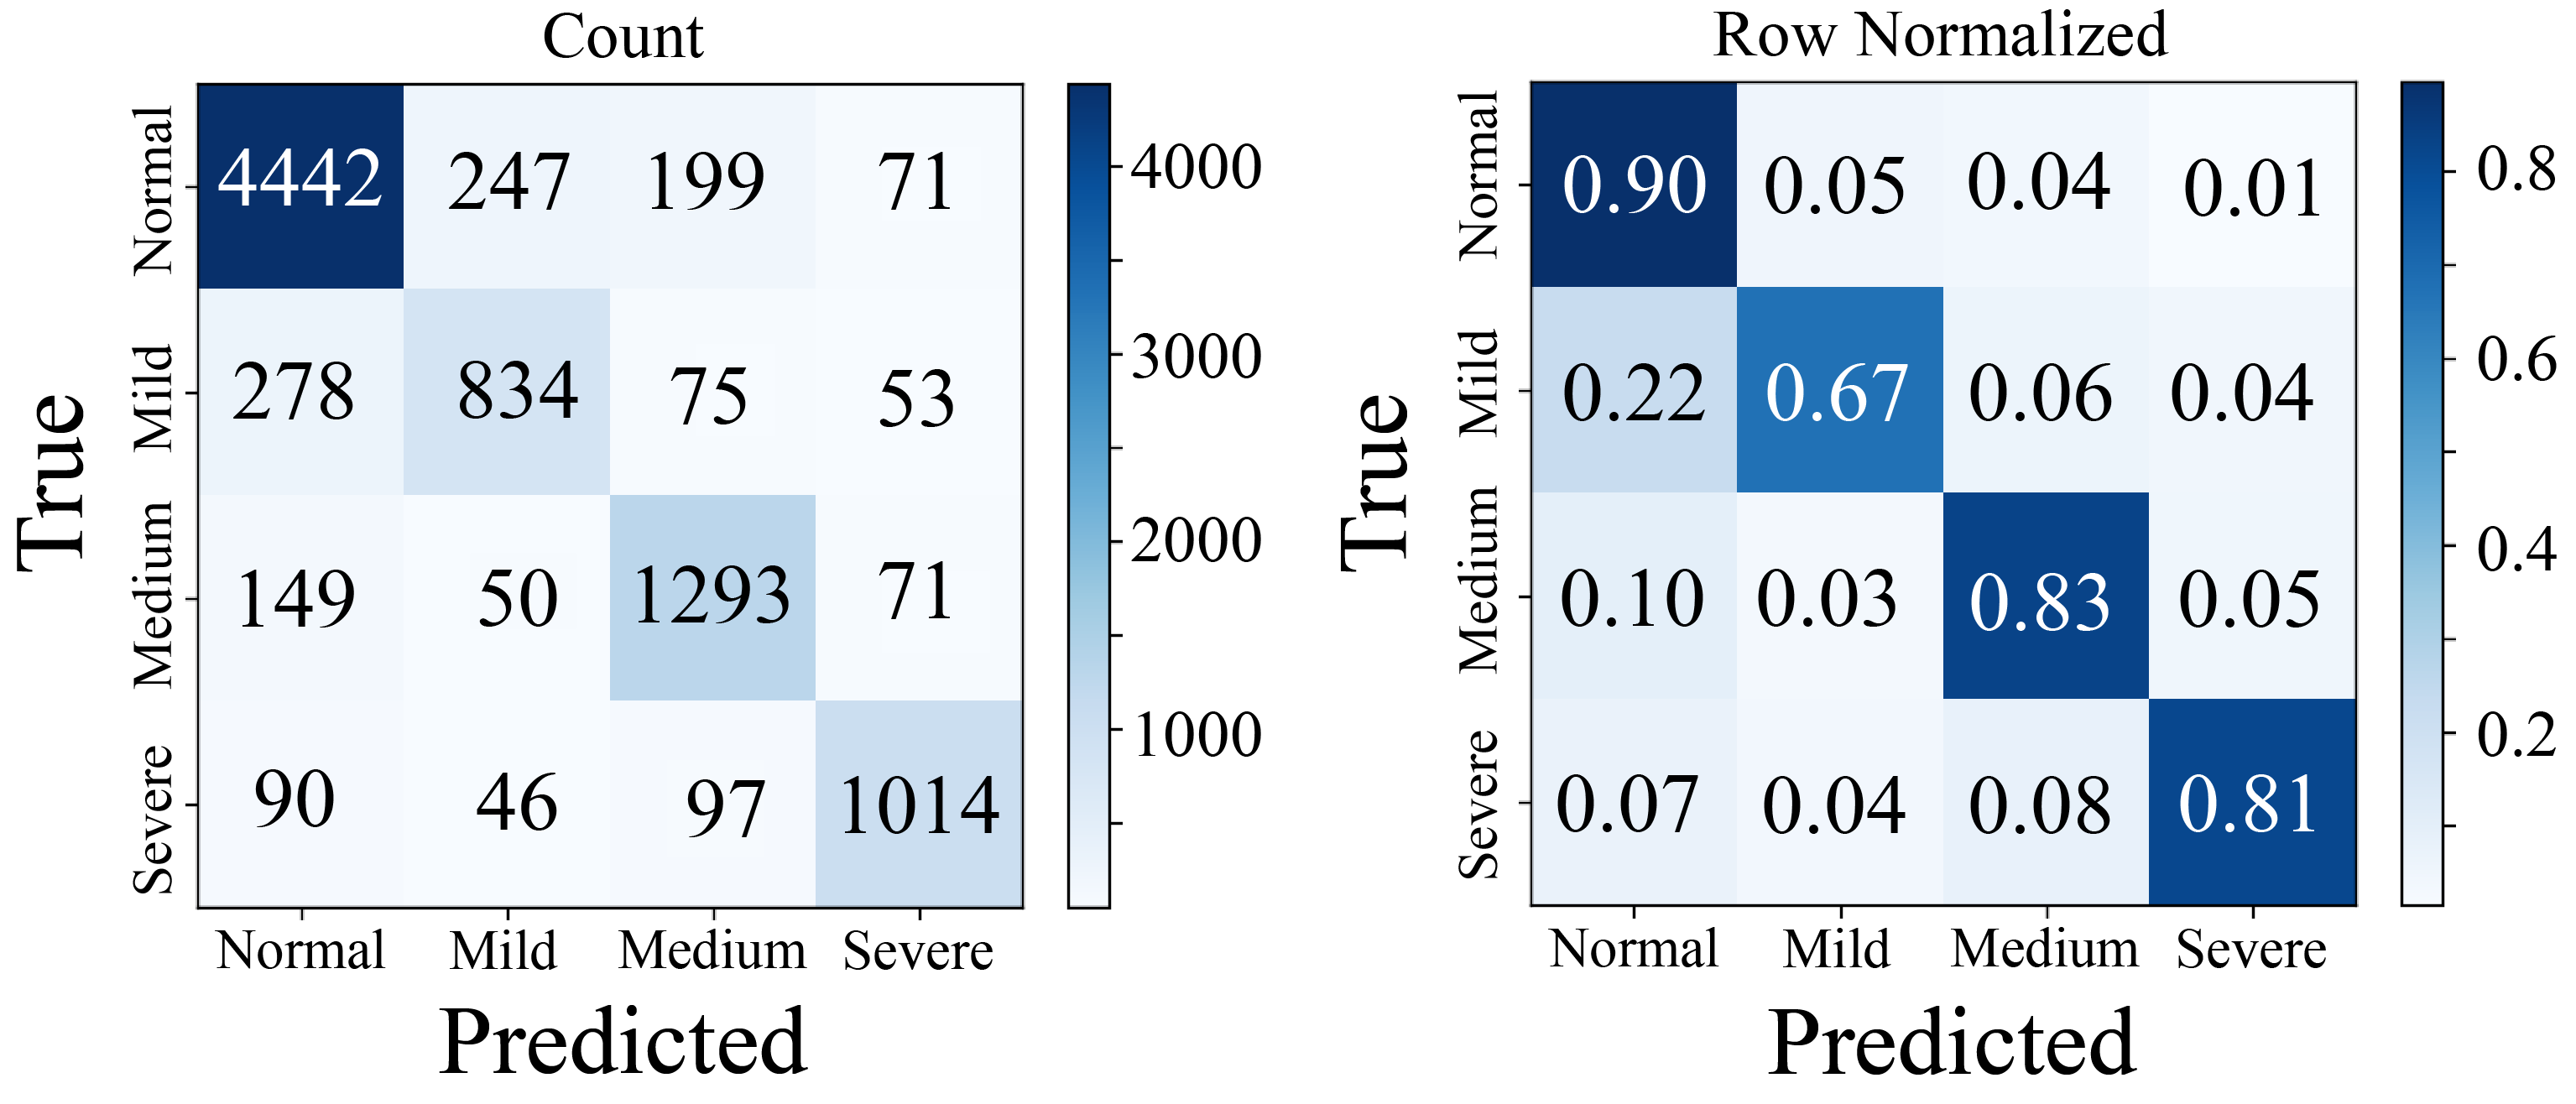
\includegraphics[width=\linewidth]{figs/severity4_pcc_confusion_revised.png}
        \vspace{-1mm}
        \centerline{(d) \texttt{severity4}, PCC stream}
    \end{minipage}

    \DiffOriginalCaption{Figure 5: In-domain confusion matrices for the proposed LF/HF InceptionTime classifier: (a) \texttt{fdia2} with motor-side measurements, (b) \texttt{fdia2} with PCC measurements, (c) \texttt{severity4} with motor-side measurements, and (d) \texttt{severity4} with PCC measurements.}


\end{minipage}\par\vspace{1em}
% Complete new block: fig:main_confusion_matrices
\begin{minipage}[t]{\DiffColumnWidth}
\centering
\textcolor{blue}{\textbf{REVISED --- Figure 5 (main\_revised.tex)}}\par\smallskip

\centering

\begingroup
\setlength{\unitlength}{1bp}
\resizebox{\linewidth}{!}{\begin{picture}(252.0000,272.0000)
\put(23.0000,205.0000){\color[rgb]{0.096348,0.400815,0.676740}\rule{52.0000bp}{52.0000bp}}
\put(49.0000,231.0000){\makebox(0,0){\color[rgb]{1,1,1}\fontsize{9.5bp}{10.5bp}\selectfont 79.1\%}}
\put(75.0000,205.0000){\color[rgb]{0.808212,0.879985,0.947835}\rule{52.0000bp}{52.0000bp}}
\put(101.0000,231.0000){\makebox(0,0){\color[rgb]{0,0,0}\fontsize{9.5bp}{10.5bp}\selectfont 20.9\%}}
\put(23.0000,153.0000){\color[rgb]{0.953249,0.974471,0.995079}\rule{52.0000bp}{52.0000bp}}
\put(49.0000,179.0000){\makebox(0,0){\color[rgb]{0,0,0}\fontsize{9.5bp}{10.5bp}\selectfont 2.3\%}}
\put(75.0000,153.0000){\color[rgb]{0.031373,0.208535,0.449750}\rule{52.0000bp}{52.0000bp}}
\put(101.0000,179.0000){\makebox(0,0){\color[rgb]{1,1,1}\fontsize{9.5bp}{10.5bp}\selectfont 97.7\%}}
\put(19.0000,231.0000){\makebox(0,0)[r]{\color[rgb]{0,0,0}\fontsize{9.5bp}{10.5bp}\selectfont N}}
\put(19.0000,179.0000){\makebox(0,0)[r]{\color[rgb]{0,0,0}\fontsize{9.5bp}{10.5bp}\selectfont A}}
\put(49.0000,145.0000){\makebox(0,0){\color[rgb]{0,0,0}\fontsize{9.5bp}{10.5bp}\selectfont N}}
\put(101.0000,145.0000){\makebox(0,0){\color[rgb]{0,0,0}\fontsize{9.5bp}{10.5bp}\selectfont A}}
\put(75.0000,266.0000){\makebox(0,0){\color[rgb]{0,0,0}\fontsize{9.5bp}{10.5bp}\selectfont (a) Motor: fdia2}}
\put(23,153){\framebox(104.0,104.0){}}
\put(146.0000,205.0000){\color[rgb]{0.047136,0.337824,0.627528}\rule{52.0000bp}{52.0000bp}}
\put(172.0000,231.0000){\makebox(0,0){\color[rgb]{1,1,1}\fontsize{9.5bp}{10.5bp}\selectfont 85.3\%}}
\put(198.0000,205.0000){\color[rgb]{0.855456,0.911480,0.963583}\rule{52.0000bp}{52.0000bp}}
\put(224.0000,231.0000){\makebox(0,0){\color[rgb]{0,0,0}\fontsize{9.5bp}{10.5bp}\selectfont 14.7\%}}
\put(146.0000,153.0000){\color[rgb]{0.778685,0.860300,0.937993}\rule{52.0000bp}{52.0000bp}}
\put(172.0000,179.0000){\makebox(0,0){\color[rgb]{0,0,0}\fontsize{9.5bp}{10.5bp}\selectfont 24.6\%}}
\put(198.0000,153.0000){\color[rgb]{0.127105,0.440185,0.707497}\rule{52.0000bp}{52.0000bp}}
\put(224.0000,179.0000){\makebox(0,0){\color[rgb]{1,1,1}\fontsize{9.5bp}{10.5bp}\selectfont 75.4\%}}
\put(142.0000,231.0000){\makebox(0,0)[r]{\color[rgb]{0,0,0}\fontsize{9.5bp}{10.5bp}\selectfont N}}
\put(142.0000,179.0000){\makebox(0,0)[r]{\color[rgb]{0,0,0}\fontsize{9.5bp}{10.5bp}\selectfont A}}
\put(172.0000,145.0000){\makebox(0,0){\color[rgb]{0,0,0}\fontsize{9.5bp}{10.5bp}\selectfont N}}
\put(224.0000,145.0000){\makebox(0,0){\color[rgb]{0,0,0}\fontsize{9.5bp}{10.5bp}\selectfont A}}
\put(198.0000,266.0000){\makebox(0,0){\color[rgb]{0,0,0}\fontsize{9.5bp}{10.5bp}\selectfont (b) PCC: fdia2}}
\put(146,153){\framebox(104.0,104.0){}}
\put(23.0000,92.3333){\color[rgb]{0.108651,0.416563,0.689043}\rule{34.6667bp}{34.6667bp}}
\put(40.3333,109.6667){\makebox(0,0){\color[rgb]{1,1,1}\fontsize{9.5bp}{10.5bp}\selectfont 77.5\%}}
\put(57.6667,92.3333){\color[rgb]{0.959400,0.978408,0.997047}\rule{34.6667bp}{34.6667bp}}
\put(75.0000,109.6667){\makebox(0,0){\color[rgb]{0,0,0}\fontsize{9.5bp}{10.5bp}\selectfont 1.3\%}}
\put(92.3333,92.3333){\color[rgb]{0.805260,0.878016,0.946851}\rule{34.6667bp}{34.6667bp}}
\put(109.6667,109.6667){\makebox(0,0){\color[rgb]{0,0,0}\fontsize{9.5bp}{10.5bp}\selectfont 21.2\%}}
\put(23.0000,57.6667){\color[rgb]{0.953249,0.974471,0.995079}\rule{34.6667bp}{34.6667bp}}
\put(40.3333,75.0000){\makebox(0,0){\color[rgb]{0,0,0}\fontsize{9.5bp}{10.5bp}\selectfont 2.3\%}}
\put(57.6667,57.6667){\color[rgb]{0.031373,0.208535,0.449750}\rule{34.6667bp}{34.6667bp}}
\put(75.0000,75.0000){\makebox(0,0){\color[rgb]{1,1,1}\fontsize{9.5bp}{10.5bp}\selectfont 97.7\%}}
\put(92.3333,57.6667){\color[rgb]{0.968627,0.984314,1.000000}\rule{34.6667bp}{34.6667bp}}
\put(109.6667,75.0000){\makebox(0,0){\color[rgb]{0,0,0}\fontsize{9.5bp}{10.5bp}\selectfont 0.0\%}}
\put(23.0000,23.0000){\color[rgb]{0.919416,0.952818,0.984252}\rule{34.6667bp}{34.6667bp}}
\put(40.3333,40.3333){\makebox(0,0){\color[rgb]{0,0,0}\fontsize{9.5bp}{10.5bp}\selectfont 6.3\%}}
\put(57.6667,23.0000){\color[rgb]{0.968627,0.984314,1.000000}\rule{34.6667bp}{34.6667bp}}
\put(75.0000,40.3333){\makebox(0,0){\color[rgb]{0,0,0}\fontsize{9.5bp}{10.5bp}\selectfont 0.0\%}}
\put(92.3333,23.0000){\color[rgb]{0.031373,0.253195,0.516063}\rule{34.6667bp}{34.6667bp}}
\put(109.6667,40.3333){\makebox(0,0){\color[rgb]{1,1,1}\fontsize{9.5bp}{10.5bp}\selectfont 93.7\%}}
\put(19.0000,109.6667){\makebox(0,0)[r]{\color[rgb]{0,0,0}\fontsize{9.5bp}{10.5bp}\selectfont N}}
\put(40.3333,15.0000){\makebox(0,0){\color[rgb]{0,0,0}\fontsize{9.5bp}{10.5bp}\selectfont N}}
\put(19.0000,75.0000){\makebox(0,0)[r]{\color[rgb]{0,0,0}\fontsize{9.5bp}{10.5bp}\selectfont AC}}
\put(75.0000,15.0000){\makebox(0,0){\color[rgb]{0,0,0}\fontsize{9.5bp}{10.5bp}\selectfont AC}}
\put(19.0000,40.3333){\makebox(0,0)[r]{\color[rgb]{0,0,0}\fontsize{9.5bp}{10.5bp}\selectfont PM}}
\put(109.6667,15.0000){\makebox(0,0){\color[rgb]{0,0,0}\fontsize{9.5bp}{10.5bp}\selectfont PM}}
\put(75.0000,136.0000){\makebox(0,0){\color[rgb]{0,0,0}\fontsize{9.5bp}{10.5bp}\selectfont (c) Motor: fdia3}}
\put(23,23){\framebox(104.0,104.0){}}
\put(146.0000,92.3333){\color[rgb]{0.211626,0.525352,0.752157}\rule{34.6667bp}{34.6667bp}}
\put(163.3333,109.6667){\makebox(0,0){\color[rgb]{1,1,1}\fontsize{9.5bp}{10.5bp}\selectfont 67.0\%}}
\put(180.6667,92.3333){\color[rgb]{0.953249,0.974471,0.995079}\rule{34.6667bp}{34.6667bp}}
\put(198.0000,109.6667){\makebox(0,0){\color[rgb]{0,0,0}\fontsize{9.5bp}{10.5bp}\selectfont 2.0\%}}
\put(215.3333,92.3333){\color[rgb]{0.701423,0.826928,0.910988}\rule{34.6667bp}{34.6667bp}}
\put(232.6667,109.6667){\makebox(0,0){\color[rgb]{0,0,0}\fontsize{9.5bp}{10.5bp}\selectfont 31.0\%}}
\put(146.0000,57.6667){\color[rgb]{0.900961,0.941007,0.978347}\rule{34.6667bp}{34.6667bp}}
\put(163.3333,75.0000){\makebox(0,0){\color[rgb]{0,0,0}\fontsize{9.5bp}{10.5bp}\selectfont 8.7\%}}
\put(180.6667,57.6667){\color[rgb]{0.031373,0.289735,0.570319}\rule{34.6667bp}{34.6667bp}}
\put(198.0000,75.0000){\makebox(0,0){\color[rgb]{1,1,1}\fontsize{9.5bp}{10.5bp}\selectfont 90.1\%}}
\put(215.3333,57.6667){\color[rgb]{0.962476,0.980377,0.998032}\rule{34.6667bp}{34.6667bp}}
\put(232.6667,75.0000){\makebox(0,0){\color[rgb]{0,0,0}\fontsize{9.5bp}{10.5bp}\selectfont 1.2\%}}
\put(146.0000,23.0000){\color[rgb]{0.796401,0.872111,0.943899}\rule{34.6667bp}{34.6667bp}}
\put(163.3333,40.3333){\makebox(0,0){\color[rgb]{0,0,0}\fontsize{9.5bp}{10.5bp}\selectfont 22.6\%}}
\put(180.6667,23.0000){\color[rgb]{0.962476,0.980377,0.998032}\rule{34.6667bp}{34.6667bp}}
\put(198.0000,40.3333){\makebox(0,0){\color[rgb]{0,0,0}\fontsize{9.5bp}{10.5bp}\selectfont 0.9\%}}
\put(215.3333,23.0000){\color[rgb]{0.117878,0.428374,0.698270}\rule{34.6667bp}{34.6667bp}}
\put(232.6667,40.3333){\makebox(0,0){\color[rgb]{1,1,1}\fontsize{9.5bp}{10.5bp}\selectfont 76.5\%}}
\put(142.0000,109.6667){\makebox(0,0)[r]{\color[rgb]{0,0,0}\fontsize{9.5bp}{10.5bp}\selectfont N}}
\put(163.3333,15.0000){\makebox(0,0){\color[rgb]{0,0,0}\fontsize{9.5bp}{10.5bp}\selectfont N}}
\put(142.0000,75.0000){\makebox(0,0)[r]{\color[rgb]{0,0,0}\fontsize{9.5bp}{10.5bp}\selectfont AC}}
\put(198.0000,15.0000){\makebox(0,0){\color[rgb]{0,0,0}\fontsize{9.5bp}{10.5bp}\selectfont AC}}
\put(142.0000,40.3333){\makebox(0,0)[r]{\color[rgb]{0,0,0}\fontsize{9.5bp}{10.5bp}\selectfont PM}}
\put(232.6667,15.0000){\makebox(0,0){\color[rgb]{0,0,0}\fontsize{9.5bp}{10.5bp}\selectfont PM}}
\put(198.0000,136.0000){\makebox(0,0){\color[rgb]{0,0,0}\fontsize{9.5bp}{10.5bp}\selectfont (d) PCC: fdia3}}
\put(146,23){\framebox(104.0,104.0){}}
\put(4.0000,140.0000){\makebox(0,0){\rotatebox{90}{\color[rgb]{0,0,0}\fontsize{9.5bp}{10.5bp}\selectfont Actual class}}}
\put(136.0000,1.0000){\makebox(0,0){\color[rgb]{0,0,0}\fontsize{9.5bp}{10.5bp}\selectfont Predicted class}}
\end{picture}}
\endgroup
\caption{Detection and motor localization: (a), (b) \texttt{fdia2}; (c), (d) \texttt{fdia3}. Cells show row percentages pooled over three holdouts. N: neither motor attacked; A: any attack; AC: ACIM attacked; PM: PMSM attacked.}
\label{fig:main_confusion_matrices}

\end{minipage}
\end{minipage}
\end{adjustbox}
\end{figure*}






\begin{figure*}[p]
\centering
\begin{adjustbox}{max width=\textwidth,max totalheight=0.87\textheight}
\begin{minipage}{\textwidth}
\centering
% Complete new block: fig:severity_detection_decisions
\begin{minipage}[t]{\DiffColumnWidth}
\centering
\textcolor{blue}{\textbf{REVISED --- Figure 6 (main\_revised.tex)}}\par\smallskip

\centering
\begingroup
\setlength{\unitlength}{1bp}
\resizebox{\linewidth}{!}{\begin{picture}(252.0000,272.0000)
\put(23.0000,231.0000){\color[rgb]{0.080969,0.381130,0.661361}\rule{26.0000bp}{26.0000bp}}
\put(36.0000,244.0000){\makebox(0,0){\color[rgb]{1,1,1}\fontsize{9.5bp}{10.5bp}\selectfont 81.2\%}}
\put(49.0000,231.0000){\color[rgb]{0.828881,0.893764,0.954725}\rule{26.0000bp}{26.0000bp}}
\put(62.0000,244.0000){\makebox(0,0){\color[rgb]{0,0,0}\fontsize{9.5bp}{10.5bp}\selectfont 18.3\%}}
\put(75.0000,231.0000){\color[rgb]{0.968627,0.984314,1.000000}\rule{26.0000bp}{26.0000bp}}
\put(88.0000,244.0000){\makebox(0,0){\color[rgb]{0,0,0}\fontsize{9.5bp}{10.5bp}\selectfont 0.2\%}}
\put(101.0000,231.0000){\color[rgb]{0.968627,0.984314,1.000000}\rule{26.0000bp}{26.0000bp}}
\put(114.0000,244.0000){\makebox(0,0){\color[rgb]{0,0,0}\fontsize{9.5bp}{10.5bp}\selectfont 0.3\%}}
\put(23.0000,205.0000){\color[rgb]{0.934794,0.962661,0.989173}\rule{26.0000bp}{26.0000bp}}
\put(36.0000,218.0000){\makebox(0,0){\color[rgb]{0,0,0}\fontsize{9.5bp}{10.5bp}\selectfont 4.4\%}}
\put(49.0000,205.0000){\color[rgb]{0.031373,0.293795,0.576348}\rule{26.0000bp}{26.0000bp}}
\put(62.0000,218.0000){\makebox(0,0){\color[rgb]{1,1,1}\fontsize{9.5bp}{10.5bp}\selectfont 89.6\%}}
\put(75.0000,205.0000){\color[rgb]{0.922491,0.954787,0.985236}\rule{26.0000bp}{26.0000bp}}
\put(88.0000,218.0000){\makebox(0,0){\color[rgb]{0,0,0}\fontsize{9.5bp}{10.5bp}\selectfont 6.0\%}}
\put(101.0000,205.0000){\color[rgb]{0.968627,0.984314,1.000000}\rule{26.0000bp}{26.0000bp}}
\put(114.0000,218.0000){\makebox(0,0){\color[rgb]{0,0,0}\fontsize{9.5bp}{10.5bp}\selectfont 0.0\%}}
\put(23.0000,179.0000){\color[rgb]{0.968627,0.984314,1.000000}\rule{26.0000bp}{26.0000bp}}
\put(36.0000,192.0000){\makebox(0,0){\color[rgb]{0,0,0}\fontsize{9.5bp}{10.5bp}\selectfont 0.3\%}}
\put(49.0000,179.0000){\color[rgb]{0.953249,0.974471,0.995079}\rule{26.0000bp}{26.0000bp}}
\put(62.0000,192.0000){\makebox(0,0){\color[rgb]{0,0,0}\fontsize{9.5bp}{10.5bp}\selectfont 2.0\%}}
\put(75.0000,179.0000){\color[rgb]{0.031373,0.249135,0.510035}\rule{26.0000bp}{26.0000bp}}
\put(88.0000,192.0000){\makebox(0,0){\color[rgb]{1,1,1}\fontsize{9.5bp}{10.5bp}\selectfont 94.0\%}}
\put(101.0000,179.0000){\color[rgb]{0.940946,0.966597,0.991142}\rule{26.0000bp}{26.0000bp}}
\put(114.0000,192.0000){\makebox(0,0){\color[rgb]{0,0,0}\fontsize{9.5bp}{10.5bp}\selectfont 3.7\%}}
\put(23.0000,153.0000){\color[rgb]{0.968627,0.984314,1.000000}\rule{26.0000bp}{26.0000bp}}
\put(36.0000,166.0000){\makebox(0,0){\color[rgb]{0,0,0}\fontsize{9.5bp}{10.5bp}\selectfont 0.4\%}}
\put(49.0000,153.0000){\color[rgb]{0.968627,0.984314,1.000000}\rule{26.0000bp}{26.0000bp}}
\put(62.0000,166.0000){\makebox(0,0){\color[rgb]{0,0,0}\fontsize{9.5bp}{10.5bp}\selectfont 0.3\%}}
\put(75.0000,153.0000){\color[rgb]{0.965552,0.982345,0.999016}\rule{26.0000bp}{26.0000bp}}
\put(88.0000,166.0000){\makebox(0,0){\color[rgb]{0,0,0}\fontsize{9.5bp}{10.5bp}\selectfont 0.6\%}}
\put(101.0000,153.0000){\color[rgb]{0.031373,0.200415,0.437693}\rule{26.0000bp}{26.0000bp}}
\put(114.0000,166.0000){\makebox(0,0){\color[rgb]{1,1,1}\fontsize{9.5bp}{10.5bp}\selectfont 98.8\%}}
\put(19.0000,244.0000){\makebox(0,0)[r]{\color[rgb]{0,0,0}\fontsize{9.5bp}{10.5bp}\selectfont N}}
\put(19.0000,218.0000){\makebox(0,0)[r]{\color[rgb]{0,0,0}\fontsize{9.5bp}{10.5bp}\selectfont L}}
\put(19.0000,192.0000){\makebox(0,0)[r]{\color[rgb]{0,0,0}\fontsize{9.5bp}{10.5bp}\selectfont M}}
\put(19.0000,166.0000){\makebox(0,0)[r]{\color[rgb]{0,0,0}\fontsize{9.5bp}{10.5bp}\selectfont H}}
\put(36.0000,145.0000){\makebox(0,0){\color[rgb]{0,0,0}\fontsize{9.5bp}{10.5bp}\selectfont N}}
\put(62.0000,145.0000){\makebox(0,0){\color[rgb]{0,0,0}\fontsize{9.5bp}{10.5bp}\selectfont L}}
\put(88.0000,145.0000){\makebox(0,0){\color[rgb]{0,0,0}\fontsize{9.5bp}{10.5bp}\selectfont M}}
\put(114.0000,145.0000){\makebox(0,0){\color[rgb]{0,0,0}\fontsize{9.5bp}{10.5bp}\selectfont H}}
\put(75.0000,266.0000){\makebox(0,0){\color[rgb]{0,0,0}\fontsize{9.5bp}{10.5bp}\selectfont (a) Motor: severity4}}
\put(23,153.0000){\framebox(104.0,104.0){}}
\put(146.0000,231.0000){\color[rgb]{0.256286,0.570012,0.775163}\rule{26.0000bp}{26.0000bp}}
\put(159.0000,244.0000){\makebox(0,0){\color[rgb]{1,1,1}\fontsize{9.5bp}{10.5bp}\selectfont 62.7\%}}
\put(172.0000,231.0000){\color[rgb]{0.811165,0.881953,0.948820}\rule{26.0000bp}{26.0000bp}}
\put(185.0000,244.0000){\makebox(0,0){\color[rgb]{0,0,0}\fontsize{9.5bp}{10.5bp}\selectfont 20.4\%}}
\put(198.0000,231.0000){\color[rgb]{0.907113,0.944944,0.980315}\rule{26.0000bp}{26.0000bp}}
\put(211.0000,244.0000){\makebox(0,0){\color[rgb]{0,0,0}\fontsize{9.5bp}{10.5bp}\selectfont 7.9\%}}
\put(224.0000,231.0000){\color[rgb]{0.897885,0.939039,0.977363}\rule{26.0000bp}{26.0000bp}}
\put(237.0000,244.0000){\makebox(0,0){\color[rgb]{0,0,0}\fontsize{9.5bp}{10.5bp}\selectfont 9.0\%}}
\put(146.0000,205.0000){\color[rgb]{0.604706,0.783975,0.879139}\rule{26.0000bp}{26.0000bp}}
\put(159.0000,218.0000){\makebox(0,0){\color[rgb]{0,0,0}\fontsize{9.5bp}{10.5bp}\selectfont 38.6\%}}
\put(172.0000,205.0000){\color[rgb]{0.604706,0.783975,0.879139}\rule{26.0000bp}{26.0000bp}}
\put(185.0000,218.0000){\makebox(0,0){\color[rgb]{0,0,0}\fontsize{9.5bp}{10.5bp}\selectfont 38.3\%}}
\put(198.0000,205.0000){\color[rgb]{0.867266,0.919354,0.967520}\rule{26.0000bp}{26.0000bp}}
\put(211.0000,218.0000){\makebox(0,0){\color[rgb]{0,0,0}\fontsize{9.5bp}{10.5bp}\selectfont 13.2\%}}
\put(224.0000,205.0000){\color[rgb]{0.891734,0.935102,0.975394}\rule{26.0000bp}{26.0000bp}}
\put(237.0000,218.0000){\makebox(0,0){\color[rgb]{0,0,0}\fontsize{9.5bp}{10.5bp}\selectfont 9.8\%}}
\put(146.0000,179.0000){\color[rgb]{0.852503,0.909512,0.962599}\rule{26.0000bp}{26.0000bp}}
\put(159.0000,192.0000){\makebox(0,0){\color[rgb]{0,0,0}\fontsize{9.5bp}{10.5bp}\selectfont 14.9\%}}
\put(172.0000,179.0000){\color[rgb]{0.876355,0.925260,0.970473}\rule{26.0000bp}{26.0000bp}}
\put(185.0000,192.0000){\makebox(0,0){\color[rgb]{0,0,0}\fontsize{9.5bp}{10.5bp}\selectfont 12.0\%}}
\put(198.0000,179.0000){\color[rgb]{0.412042,0.677186,0.836263}\rule{26.0000bp}{26.0000bp}}
\put(211.0000,192.0000){\makebox(0,0){\color[rgb]{0,0,0}\fontsize{9.5bp}{10.5bp}\selectfont 50.6\%}}
\put(224.0000,179.0000){\color[rgb]{0.796401,0.872111,0.943899}\rule{26.0000bp}{26.0000bp}}
\put(237.0000,192.0000){\makebox(0,0){\color[rgb]{0,0,0}\fontsize{9.5bp}{10.5bp}\selectfont 22.5\%}}
\put(146.0000,153.0000){\color[rgb]{0.876355,0.925260,0.970473}\rule{26.0000bp}{26.0000bp}}
\put(159.0000,166.0000){\makebox(0,0){\color[rgb]{0,0,0}\fontsize{9.5bp}{10.5bp}\selectfont 11.9\%}}
\put(172.0000,153.0000){\color[rgb]{0.907113,0.944944,0.980315}\rule{26.0000bp}{26.0000bp}}
\put(185.0000,166.0000){\makebox(0,0){\color[rgb]{0,0,0}\fontsize{9.5bp}{10.5bp}\selectfont 8.1\%}}
\put(198.0000,153.0000){\color[rgb]{0.897885,0.939039,0.977363}\rule{26.0000bp}{26.0000bp}}
\put(211.0000,166.0000){\makebox(0,0){\color[rgb]{0,0,0}\fontsize{9.5bp}{10.5bp}\selectfont 9.2\%}}
\put(224.0000,153.0000){\color[rgb]{0.171027,0.484752,0.731242}\rule{26.0000bp}{26.0000bp}}
\put(237.0000,166.0000){\makebox(0,0){\color[rgb]{1,1,1}\fontsize{9.5bp}{10.5bp}\selectfont 70.8\%}}
\put(142.0000,244.0000){\makebox(0,0)[r]{\color[rgb]{0,0,0}\fontsize{9.5bp}{10.5bp}\selectfont N}}
\put(142.0000,218.0000){\makebox(0,0)[r]{\color[rgb]{0,0,0}\fontsize{9.5bp}{10.5bp}\selectfont L}}
\put(142.0000,192.0000){\makebox(0,0)[r]{\color[rgb]{0,0,0}\fontsize{9.5bp}{10.5bp}\selectfont M}}
\put(142.0000,166.0000){\makebox(0,0)[r]{\color[rgb]{0,0,0}\fontsize{9.5bp}{10.5bp}\selectfont H}}
\put(159.0000,145.0000){\makebox(0,0){\color[rgb]{0,0,0}\fontsize{9.5bp}{10.5bp}\selectfont N}}
\put(185.0000,145.0000){\makebox(0,0){\color[rgb]{0,0,0}\fontsize{9.5bp}{10.5bp}\selectfont L}}
\put(211.0000,145.0000){\makebox(0,0){\color[rgb]{0,0,0}\fontsize{9.5bp}{10.5bp}\selectfont M}}
\put(237.0000,145.0000){\makebox(0,0){\color[rgb]{0,0,0}\fontsize{9.5bp}{10.5bp}\selectfont H}}
\put(198.0000,266.0000){\makebox(0,0){\color[rgb]{0,0,0}\fontsize{9.5bp}{10.5bp}\selectfont (b) PCC: severity4}}
\put(146,153.0000){\framebox(104.0,104.0){}}

\put(23.0000,101.0000){\color[rgb]{0.256286,0.570012,0.775163}\rule{48.0000bp}{26.0000bp}}
\put(47.0000,114.0000){\makebox(0,0){\color[rgb]{1,1,1}\fontsize{9.5bp}{10.5bp}\selectfont 62.7\%}}
\put(71.0000,101.0000){\color[rgb]{0.622684,0.793464,0.883429}\rule{48.0000bp}{26.0000bp}}
\put(95.0000,114.0000){\makebox(0,0){\color[rgb]{0,0,0}\fontsize{9.5bp}{10.5bp}\selectfont 37.3\%}}
\put(23.0000,75.0000){\color[rgb]{0.604706,0.783975,0.879139}\rule{48.0000bp}{26.0000bp}}
\put(47.0000,88.0000){\makebox(0,0){\color[rgb]{0,0,0}\fontsize{9.5bp}{10.5bp}\selectfont 38.6\%}}
\put(71.0000,75.0000){\color[rgb]{0.270804,0.580730,0.781146}\rule{48.0000bp}{26.0000bp}}
\put(95.0000,88.0000){\makebox(0,0){\color[rgb]{1,1,1}\fontsize{9.5bp}{10.5bp}\selectfont 61.4\%}}
\put(23.0000,49.0000){\color[rgb]{0.852503,0.909512,0.962599}\rule{48.0000bp}{26.0000bp}}
\put(47.0000,62.0000){\makebox(0,0){\color[rgb]{0,0,0}\fontsize{9.5bp}{10.5bp}\selectfont 14.9\%}}
\put(71.0000,49.0000){\color[rgb]{0.050211,0.341761,0.630604}\rule{48.0000bp}{26.0000bp}}
\put(95.0000,62.0000){\makebox(0,0){\color[rgb]{1,1,1}\fontsize{9.5bp}{10.5bp}\selectfont 85.1\%}}
\put(23.0000,23.0000){\color[rgb]{0.876355,0.925260,0.970473}\rule{48.0000bp}{26.0000bp}}
\put(47.0000,36.0000){\makebox(0,0){\color[rgb]{0,0,0}\fontsize{9.5bp}{10.5bp}\selectfont 11.9\%}}
\put(71.0000,23.0000){\color[rgb]{0.031373,0.310035,0.600461}\rule{48.0000bp}{26.0000bp}}
\put(95.0000,36.0000){\makebox(0,0){\color[rgb]{1,1,1}\fontsize{9.5bp}{10.5bp}\selectfont 88.1\%}}
\put(19.0000,114.0000){\makebox(0,0)[r]{\color[rgb]{0,0,0}\fontsize{9.5bp}{10.5bp}\selectfont N}}
\put(19.0000,88.0000){\makebox(0,0)[r]{\color[rgb]{0,0,0}\fontsize{9.5bp}{10.5bp}\selectfont L}}
\put(19.0000,62.0000){\makebox(0,0)[r]{\color[rgb]{0,0,0}\fontsize{9.5bp}{10.5bp}\selectfont M}}
\put(19.0000,36.0000){\makebox(0,0)[r]{\color[rgb]{0,0,0}\fontsize{9.5bp}{10.5bp}\selectfont H}}
\put(47.0000,15.0000){\makebox(0,0){\color[rgb]{0,0,0}\fontsize{9.5bp}{10.5bp}\selectfont N}}
\put(95.0000,15.0000){\makebox(0,0){\color[rgb]{0,0,0}\fontsize{9.5bp}{10.5bp}\selectfont A}}
\put(71.0000,136.0000){\makebox(0,0){\color[rgb]{0,0,0}\fontsize{9.5bp}{10.5bp}\selectfont (c) PCC: by true class}}
\put(23,23){\framebox(96,104){}}
\put(148.0000,75.0000){\color[rgb]{0.256286,0.570012,0.775163}\rule{48.0000bp}{26.0000bp}}
\put(172.0000,88.0000){\makebox(0,0){\color[rgb]{1,1,1}\fontsize{9.5bp}{10.5bp}\selectfont 62.7\%}}
\put(196.0000,75.0000){\color[rgb]{0.622684,0.793464,0.883429}\rule{48.0000bp}{26.0000bp}}
\put(220.0000,88.0000){\makebox(0,0){\color[rgb]{0,0,0}\fontsize{9.5bp}{10.5bp}\selectfont 37.3\%}}
\put(148.0000,49.0000){\color[rgb]{0.828881,0.893764,0.954725}\rule{48.0000bp}{26.0000bp}}
\put(172.0000,62.0000){\makebox(0,0){\color[rgb]{0,0,0}\fontsize{9.5bp}{10.5bp}\selectfont 18.1\%}}
\put(196.0000,49.0000){\color[rgb]{0.074817,0.373256,0.655210}\rule{48.0000bp}{26.0000bp}}
\put(220.0000,62.0000){\makebox(0,0){\color[rgb]{1,1,1}\fontsize{9.5bp}{10.5bp}\selectfont 82.0\%}}
\put(144.0000,88.0000){\makebox(0,0)[r]{\color[rgb]{0,0,0}\fontsize{9.5bp}{10.5bp}\selectfont N}}
\put(144.0000,62.0000){\makebox(0,0)[r]{\color[rgb]{0,0,0}\fontsize{9.5bp}{10.5bp}\selectfont A}}
\put(172.0000,41.0000){\makebox(0,0){\color[rgb]{0,0,0}\fontsize{9.5bp}{10.5bp}\selectfont N}}
\put(220.0000,41.0000){\makebox(0,0){\color[rgb]{0,0,0}\fontsize{9.5bp}{10.5bp}\selectfont A}}
\put(196.0000,110.0000){\makebox(0,0){\color[rgb]{0,0,0}\fontsize{9.5bp}{10.5bp}\selectfont (d) PCC: collapsed}}
\put(148,49){\framebox(96,52){}}
\put(4.0000,141.0000){\makebox(0,0){\rotatebox{90}{\color[rgb]{0,0,0}\fontsize{9.5bp}{10.5bp}\selectfont Actual class}}}
\put(134.0000,1.0000){\makebox(0,0){\color[rgb]{0,0,0}\fontsize{9.5bp}{10.5bp}\selectfont Predicted class}}
\end{picture}}
\endgroup
\caption{Severity assessment: (a), (b) motor and PCC four-class matrices; (c) PCC normal/attack decisions by true severity; (d) collapsed PCC normal/attack matrix. Cells show row percentages pooled over three holdouts. N: normal; L/M/H: low/medium/high bias; A: any attack. Panels (c), (d) derive from the four-class PCC model.}
\label{fig:severity_detection_decisions}

\end{minipage}
\end{minipage}
\end{adjustbox}
\end{figure*}




\DIFaddend \subsection{Comparison with Deep and Classical ML Baselines}
\label{sec:model_comparison}
\DIFaddbegin

\DIFaddend To benchmark the proposed LF/HF Inception-based model, representative deep-learning and classical \DIFdelbegin \DIFdel{ML }\DIFdelend \DIFaddbegin \DIFadd{machine-learning (ML) }\DIFaddend baselines were evaluated on the PCC-based \texttt{fdia2} and \texttt{severity4} tasks, which were the most challenging in-domain settings. The baselines include ResNet, \DIFdelbegin \DIFdel{MLSTM-FCN}\DIFdelend \DIFaddbegin \DIFadd{LSTM-FCN}\DIFaddend , Random Forest, \DIFdelbegin \DIFdel{and XGBoost, }\DIFdelend \DIFaddbegin \DIFadd{XGBoost, and MultiRocket~}\cite{tan2022multirocket}\DIFadd{, }\DIFaddend while the proposed model uses the final stream-specific InceptionTime configuration selected by validation-based hyperparameter search. \DIFaddbegin \DIFadd{All methods use the same recording partitions and feature inputs; search budgets differ between model families. }\DIFaddend As shown in Table~\ref{tab:model_comparison_hard_tasks}, the proposed model achieved the highest \DIFaddbegin \DIFadd{mean }\DIFaddend accuracy, balanced accuracy, and F1 score among the evaluated baselines \DIFdelbegin \DIFdel{on both PCC tasks. The performance gap is larger for }\DIFdelend \DIFaddbegin \DIFadd{for PCC binary detection, and the highest mean balanced accuracy for PCC severity assessment. For }\DIFaddend \texttt{severity4}\DIFdelbegin \DIFdel{, confirming that PCC-based severity discrimination is more challenging than binary FDIA detectionand benefits from the proposed temporal LF/HF representation. }\DIFdelend \DIFaddbegin \DIFadd{, XGBoost achieved higher accuracy and LSTM-FCN slightly higher macro F1. The proposed model therefore improves average class recall for PCC severity assessment, while the preferred model depends on the evaluation metric.
}



\begin{table*}[p]
\centering
\begin{adjustbox}{max width=\textwidth,max totalheight=0.87\textheight}
\begin{minipage}{\textwidth}
\centering
% Complete old block: tab:model_comparison_hard_tasks
\begin{minipage}[t]{0.48\textwidth}
\centering
\textcolor{red}{\textbf{ORIGINAL --- Table 6 (main.tex)}}\par\smallskip

\centering
\DiffOriginalCaption{Table 6: Baseline comparison on the PCC-based \texttt{fdia2} and \texttt{severity4} tasks.}

\renewcommand{\arraystretch}{1.05}
\setlength{\tabcolsep}{3pt}
\begin{adjustbox}{max width=\linewidth}\begin{tabular}{l c c c}
\hline
Method & Acc. (\%) & Balanced Acc. (\%) & F1 (\%) \\
\hline
\multicolumn{4}{c}{\textit{\texttt{fdia2}}} \\
\hline
Proposed InceptionTime & 89.44 & 88.99 & 89.25 \\
ResNet        & 85.58 & 84.83 & 85.20 \\
MLSTM-FCN     & 84.58 & 83.80 & 84.17 \\
Rand. Forest  & 86.05 & 85.27 & 85.67 \\
XGBoost       & 86.45 & 85.75 & 86.11 \\
\hline
\multicolumn{4}{c}{\textit{\texttt{severity4}}} \\
\hline
Proposed InceptionTime & 84.17 & 80.22 & 80.32 \\
ResNet        & 77.31 & 70.22 & 70.68 \\
MLSTM-FCN     & 77.96 & 71.11 & 71.89 \\
Rand. Forest  & 83.42 & 72.68 & 77.40 \\
XGBoost       & 79.00 & 65.21 & 70.45 \\
\hline
\end{tabular}\end{adjustbox}

\end{minipage}\hfill%
% Complete new block: tab:model_comparison_hard_tasks
\begin{minipage}[t]{0.48\textwidth}
\centering
\textcolor{blue}{\textbf{REVISED --- Table 6 (main\_revised.tex)}}\par\smallskip

\centering
\footnotesize
\caption{PCC baseline comparison on \texttt{fdia2} and \texttt{severity4} (\%).}
\label{tab:model_comparison_hard_tasks}
\renewcommand{\arraystretch}{1.15}
\setlength{\tabcolsep}{2.2pt}
\begin{tabular}{@{}lccc@{}}
\hline
Method & Accuracy & BA & Macro F1 \\\hline
\hline\multicolumn{4}{c}{\textit{\texttt{fdia2}}} \\\hline
InceptionTime & \mbox{\textbf{80.78}\,$\pm$\,2.95} & \mbox{\textbf{80.29}\,$\pm$\,3.03} & \mbox{\textbf{80.42}\,$\pm$\,2.96} \\
ResNet & \mbox{73.91\,$\pm$\,5.78} & \mbox{73.99\,$\pm$\,5.33} & \mbox{73.76\,$\pm$\,5.66} \\
LSTM-FCN & \mbox{72.57\,$\pm$\,4.89} & \mbox{72.52\,$\pm$\,4.31} & \mbox{72.35\,$\pm$\,4.66} \\
Rand. Forest & \mbox{70.43\,$\pm$\,1.00} & \mbox{68.69\,$\pm$\,0.74} & \mbox{68.45\,$\pm$\,0.85} \\
XGBoost & \mbox{75.37\,$\pm$\,0.81} & \mbox{73.84\,$\pm$\,1.11} & \mbox{73.97\,$\pm$\,1.17} \\
MultiRocket & \mbox{70.10\,$\pm$\,2.13} & \mbox{69.55\,$\pm$\,2.82} & \mbox{69.35\,$\pm$\,2.39} \\
\hline\multicolumn{4}{c}{\textit{\texttt{severity4}}} \\\hline
InceptionTime & \mbox{61.00\,$\pm$\,1.32} & \mbox{\textbf{55.62}\,$\pm$\,2.94} & \mbox{52.96\,$\pm$\,2.15} \\
ResNet & \mbox{65.18\,$\pm$\,5.35} & \mbox{50.41\,$\pm$\,5.44} & \mbox{51.15\,$\pm$\,5.71} \\
LSTM-FCN & \mbox{66.60\,$\pm$\,1.72} & \mbox{52.38\,$\pm$\,2.12} & \mbox{\textbf{53.23}\,$\pm$\,1.94} \\
Rand. Forest & \mbox{67.36\,$\pm$\,0.17} & \mbox{43.49\,$\pm$\,2.18} & \mbox{45.07\,$\pm$\,2.59} \\
XGBoost & \mbox{\textbf{70.45}\,$\pm$\,0.74} & \mbox{47.17\,$\pm$\,2.02} & \mbox{49.67\,$\pm$\,2.17} \\
MultiRocket & \mbox{58.41\,$\pm$\,3.34} & \mbox{44.92\,$\pm$\,3.46} & \mbox{44.28\,$\pm$\,2.52} \\
\hline\end{tabular}
\par\smallskip\begin{minipage}{\columnwidth}\scriptsize Mean $\pm$ sample SD over three holdouts. Bold: highest mean for each metric within a task; it does not indicate statistical significance.\end{minipage}

\end{minipage}
\end{minipage}
\end{adjustbox}
\end{table*}
\DIFaddend



\subsection{Cross-Domain Transfer Without Adaptation}
\label{sec:cross_domain}
\DIFdelbegin \DIFdel{Source-only transfer was evaluated by training on one motor type and testing directly on the other. Two transfer directions were considered: ACIM $\rightarrow$ PMSM and PMSM $\rightarrow$ ACIM.
}\DIFdelend \DIFaddbegin

\DIFaddend Table~\ref{tab:cross_domain_source_only} shows that source-only \DIFdelbegin \DIFdel{fdia2 }\DIFdelend \DIFaddbegin \texttt{\DIFadd{fdia2}} \DIFaddend transfer falls near chance balanced accuracy for \DIFdelbegin \DIFdel{both sensingstreams}\DIFdelend \DIFaddbegin \DIFadd{ACIM-to-PMSM transfer, while the reverse direction falls below chance for motor sensing and reaches 56.00\% for PCC sensing}\DIFaddend . For \texttt{fdia2}, the source-only results in Table~\ref{tab:cross_domain_source_only} show a substantial degradation relative to the mixed-domain baselines.
\DIFdelbegin \DIFdel{This confirms a substantial ACIM/PMSM domain shift in the tested transfer setting. Thus, reliable cross-motor FDIA detection in this setting benefits from target-domain adaptation.
}\DIFdelend \DIFaddbegin



\begin{table*}[p]
\centering
\begin{adjustbox}{max width=\textwidth,max totalheight=0.87\textheight}
\begin{minipage}{\textwidth}
\centering
% Complete old block: tab:cross_domain_source_only
\begin{minipage}[t]{0.48\textwidth}
\centering
\textcolor{red}{\textbf{ORIGINAL --- Table 7 (main.tex)}}\par\smallskip

\centering
\DiffOriginalCaption{Table 7: Cross-domain source-only performance without target-domain adaptation on \texttt{fdia2} task.}

\renewcommand{\arraystretch}{1.15}
\begin{adjustbox}{max width=\linewidth}\begin{tabular}{l l c c c c}
\hline
Stream & Direction & Accuracy (\%) & Balanced Acc. (\%) \\
\hline
Motor & ACIM $\rightarrow$ PMSM & 53.87 & 50.10 \\
Motor & PMSM $\rightarrow$ ACIM & 51.08 & 51.80 \\
PCC   & ACIM $\rightarrow$ PMSM & 54.79 & 50.07 \\
PCC   & PMSM $\rightarrow$ ACIM & 52.38 & 57.03 \\
\hline
\end{tabular}\end{adjustbox}

\end{minipage}\hfill%
% Complete new block: tab:cross_domain_source_only
\begin{minipage}[t]{0.48\textwidth}
\centering
\textcolor{blue}{\textbf{REVISED --- Table 7 (main\_revised.tex)}}\par\smallskip

\centering
\footnotesize
\caption{Source-only \texttt{fdia2} transfer without target adaptation (\%).}
\label{tab:cross_domain_source_only}
\renewcommand{\arraystretch}{1.15}
\setlength{\tabcolsep}{2.2pt}
\begin{tabular}{@{}lccc@{}}
\hline
Direction & Accuracy & BA & Macro F1 \\\hline
\hline\multicolumn{4}{c}{\textit{MOTOR stream}} \\\hline
ACIM $\to$ PMSM & \mbox{55.21\,$\pm$\,1.14} & \mbox{50.60\,$\pm$\,0.73} & \mbox{37.71\,$\pm$\,2.37} \\
PMSM $\to$ ACIM & \mbox{36.22\,$\pm$\,4.23} & \mbox{36.08\,$\pm$\,4.11} & \mbox{33.89\,$\pm$\,4.62} \\
\hline\multicolumn{4}{c}{\textit{PCC stream}} \\\hline
ACIM $\to$ PMSM & \mbox{55.88\,$\pm$\,0.64} & \mbox{51.58\,$\pm$\,1.52} & \mbox{41.13\,$\pm$\,5.84} \\
PMSM $\to$ ACIM & \mbox{51.94\,$\pm$\,6.54} & \mbox{56.00\,$\pm$\,5.69} & \mbox{43.62\,$\pm$\,11.38} \\
\hline\end{tabular}
\par\smallskip\begin{minipage}{\columnwidth}\scriptsize Mean $\pm$ sample SD over three holdouts. Directions are different target-domain tests, so no best direction is highlighted.\end{minipage}

\end{minipage}
\end{minipage}
\end{adjustbox}
\end{table*}
\DIFaddend




\subsection{Domain Adaptation Results: 1/5/10/20\%}
\label{sec:adaptation_results}
\DIFaddbegin

\DIFaddend Table~\ref{tab:domain_adaptation_anomaly2} reports \DIFdelbegin \DIFdel{fdia2 }\DIFdelend \DIFaddbegin \texttt{\DIFadd{fdia2}} \DIFaddend few-shot adaptation using \DIFaddbegin \DIFadd{nominal budgets of }\DIFaddend 1\%, 5\%, 10\%, and 20\% labeled target \DIFdelbegin \DIFdel{data. In all cases}\DIFdelend \DIFaddbegin \DIFadd{episode groups. At the 20\% budget}\DIFaddend , adaptation improved performance relative to the source-only setting \DIFaddbegin \DIFadd{in all cases}\DIFaddend , although the magnitude of the gain was strongly direction dependent. For ACIM-to-PMSM transfer, adaptation \DIFdelbegin \DIFdel{gives only modest gains, reaching 57.49}\DIFdelend \DIFaddbegin \DIFadd{reaches 75.99}\DIFaddend \% balanced accuracy for motor sensing and \DIFdelbegin \DIFdel{60.06}\DIFdelend \DIFaddbegin \DIFadd{56.30}\DIFaddend \% for PCC at 20\% target data. For PMSM-to-ACIM transfer, adaptation is much stronger, reaching \DIFdelbegin \DIFdel{86.10}\DIFdelend \DIFaddbegin \DIFadd{92.63}\DIFaddend \% balanced accuracy for motor sensing and \DIFdelbegin \DIFdel{91.16}\DIFdelend \DIFaddbegin \DIFadd{91.38}\DIFaddend \% for PCC at 20\% target data.
\DIFaddbegin \DIFadd{With only the nominal 1\% budget, PMSM-to-ACIM balanced accuracy rises from 36.08\% to 64.35\% for motor sensing and from 56.00\% to 77.43\% for PCC sensing, gains of 28.27 and 21.43 percentage points.
}

\DIFaddend Overall, the adaptation results show that few-shot target-domain fine-tuning can improve transfer performance, but the gains are strongly direction dependent and are much larger in the PMSM $\rightarrow$ ACIM direction. This asymmetry indicates that cross-motor FDIA adaptation cannot be treated as a symmetric transfer problem; in practice, the pretraining motor domain materially affects PCC deployment performance.





\DIFaddbegin \begin{table*}[p]
\centering
\begin{adjustbox}{max width=\textwidth,max totalheight=0.87\textheight}
\begin{minipage}{\textwidth}
\centering
% Complete old block: tab:domain_adaptation_anomaly2
\begin{minipage}[t]{\DiffColumnWidth}
\centering
\textcolor{red}{\textbf{ORIGINAL --- Table 8 (main.tex)}}\par\smallskip

\centering
\scriptsize
\DiffOriginalCaption{Table 8: Few-shot domain-adaptation results for \texttt{fdia2} using labeled target-domain fine-tuning. Values are mean test balanced accuracy (\%) over three seeds.}

\renewcommand{\arraystretch}{1.15}
\begin{adjustbox}{max width=\linewidth}\begin{tabular}{l l c c c c c}
\hline
Stream & Direction & Source-only & 1\% & 5\% & 10\% & 20\% \\
\hline
Motor & ACIM $\rightarrow$ PMSM & 50.10 & 50.06 & 49.63 & 53.15 & 57.49 \\
Motor & PMSM $\rightarrow$ ACIM & 51.80 & 57.95 & 73.75 & 78.86 & 86.10 \\
PCC   & ACIM $\rightarrow$ PMSM & 50.07 & 51.79 & 55.51 & 57.47 & 60.06 \\
PCC   & PMSM $\rightarrow$ ACIM & 57.03 & 70.10 & 84.56 & 89.12 & 91.16 \\
\hline
\end{tabular}\end{adjustbox}

\end{minipage}\par\vspace{1em}
% Complete new block: tab:domain_adaptation_anomaly2
\begin{minipage}[t]{\textwidth}
\centering
\textcolor{blue}{\textbf{REVISED --- Table 8 (main\_revised.tex)}}\par\smallskip

\centering
\footnotesize
\caption{Few-shot \texttt{fdia2} adaptation by labeled target-domain fine-tuning: balanced accuracy (\%).}
\label{tab:domain_adaptation_anomaly2}
\renewcommand{\arraystretch}{1.15}
\setlength{\tabcolsep}{6pt}
\begin{tabular}{@{}lccccc@{}}
\hline
Direction & Source only & 1\% & 5\% & 10\% & 20\% \\\hline
\hline\multicolumn{6}{c}{\textit{MOTOR stream}} \\\hline
ACIM $\to$ PMSM & \mbox{50.60\,$\pm$\,0.73} & \mbox{50.43\,$\pm$\,1.74} & \mbox{53.83\,$\pm$\,1.14} & \mbox{57.51\,$\pm$\,7.24} & \mbox{\textbf{75.99}\,$\pm$\,1.73} \\
PMSM $\to$ ACIM & \mbox{36.08\,$\pm$\,4.11} & \mbox{64.35\,$\pm$\,9.23} & \mbox{73.93\,$\pm$\,8.78} & \mbox{88.04\,$\pm$\,5.36} & \mbox{\textbf{92.63}\,$\pm$\,3.72} \\
\hline\multicolumn{6}{c}{\textit{PCC stream}} \\\hline
ACIM $\to$ PMSM & \mbox{51.58\,$\pm$\,1.52} & \mbox{54.01\,$\pm$\,0.12} & \mbox{54.62\,$\pm$\,1.76} & \mbox{54.04\,$\pm$\,1.35} & \mbox{\textbf{56.30}\,$\pm$\,3.23} \\
PMSM $\to$ ACIM & \mbox{56.00\,$\pm$\,5.69} & \mbox{77.43\,$\pm$\,10.43} & \mbox{84.22\,$\pm$\,4.62} & \mbox{86.72\,$\pm$\,4.37} & \mbox{\textbf{91.38}\,$\pm$\,2.06} \\
\hline\end{tabular}
\par\smallskip\begin{minipage}{\textwidth}\scriptsize Mean $\pm$ sample SD over three holdouts. Bold: highest observed mean within each direction and stream; no test-based configuration selection. Budgets refer to the target episode-group pool.\end{minipage}

\end{minipage}
\end{minipage}
\end{adjustbox}
\end{table*}




\DIFaddend \subsection{Error Analysis: Confusion Matrices and FP/FN Behavior}
\label{sec:error_analysis}
\DIFaddbegin

\DIFaddend Fig.~\ref{fig:main_confusion_matrices} compares the in-domain confusion matrices for \texttt{fdia2} and \texttt{\DIFdelbegin \DIFdel{severity4}\DIFdelend \DIFaddbegin \DIFadd{fdia3}\DIFaddend }. For \texttt{fdia2}, motor-side sensing yields a strongly diagonal confusion matrix \DIFdelbegin \DIFdel{with low }\DIFdelend \DIFaddbegin \DIFadd{for attack windows, with pooled }\DIFaddend false-positive \DIFaddbegin \DIFadd{(FP) }\DIFaddend and false-negative \DIFdelbegin \DIFdel{rates of 0.75\% and 1.56}\DIFdelend \DIFaddbegin \DIFadd{(FN) rates of 20.9\% and 2.3}\DIFaddend \%, respectively\DIFdelbegin \DIFdel{, whereas PCC sensing increases these rates to 6.55\% and 15.46\% because the attack is observed only through the aggregated current response}\DIFdelend \DIFaddbegin \DIFadd{. PCC sensing yields 14.7\% false positives and 24.6\% false negatives, showing fewer false alarms but more missed attacks. The }\texttt{\DIFadd{fdia3}} \DIFadd{matrices show that false alarms and missed attacks are more frequent than confusion between the attacked motor types. Mean normal false-alarm rates are 22.85\% for motor sensing and 33.12\% for PCC sensing}\DIFaddend . For \texttt{severity4} \DIFaddbegin \DIFadd{in Fig.~\ref{fig:severity_detection_decisions}(a), (b)}\DIFaddend , PCC errors \DIFdelbegin \DIFdel{concentrate between adjacent classes, especially }\DIFdelend \DIFaddbegin \DIFadd{include both }\DIFaddend normal/\DIFdelbegin \DIFdel{mild and mild/medium}\DIFdelend \DIFaddbegin \DIFadd{attack confusion and confusion among the nonzero bias classes}\DIFaddend , indicating that PCC measurements retain coarse attack information but blur finer severity distinctions.

Fig.~\ref{fig:case1_30_motor_pcc_detection_examples} complements the aggregate confusion-matrix results by showing a representative \DIFaddbegin \DIFadd{held-out }\DIFaddend ACIM detection sequence on a continuous experimental signal. \DIFdelbegin \DIFdel{Both sensing locations follow the }\DIFdelend \DIFaddbegin \DIFadd{The motor-side detector follows most }\DIFaddend scheduled normal/FDIA intervals, \DIFdelbegin \DIFdel{but the motor-side detector produces cleaner transitions than }\DIFdelend \DIFaddbegin \DIFadd{while }\DIFaddend the PCC-side detector \DIFaddbegin \DIFadd{exhibits missed attacks and false alarms}\DIFaddend , especially near the first \DIFdelbegin \DIFdel{attack onset and low-severity FDIA intervals}\DIFdelend \DIFaddbegin \DIFadd{low-bias attack}\DIFaddend . These results indicate that motor-side measurements are more separable, while PCC measurements remain useful but less reliable for \DIFdelbegin \DIFdel{fine severity discrimination}\DIFdelend \DIFaddbegin \DIFadd{detecting small attacks. Root-mean-square (RMS) traces use 500-sample frames at stride 25, and predictions are placed at window ends. Green curves show attack probability, red curves show predicted labels, and dashed gray curves show true labels; the dotted threshold is 0.5}\DIFaddend .



\DIFaddbegin \begin{figure*}[p]
\centering
\begin{adjustbox}{max width=\textwidth,max totalheight=0.87\textheight}
\begin{minipage}{\textwidth}
\centering
% Complete old block: fig:case1_30_motor_pcc_detection_examples
\begin{minipage}[t]{\DiffColumnWidth}
\centering
\textcolor{red}{\textbf{ORIGINAL --- Figure 6 (main.tex)}}\par\smallskip

    \centering
    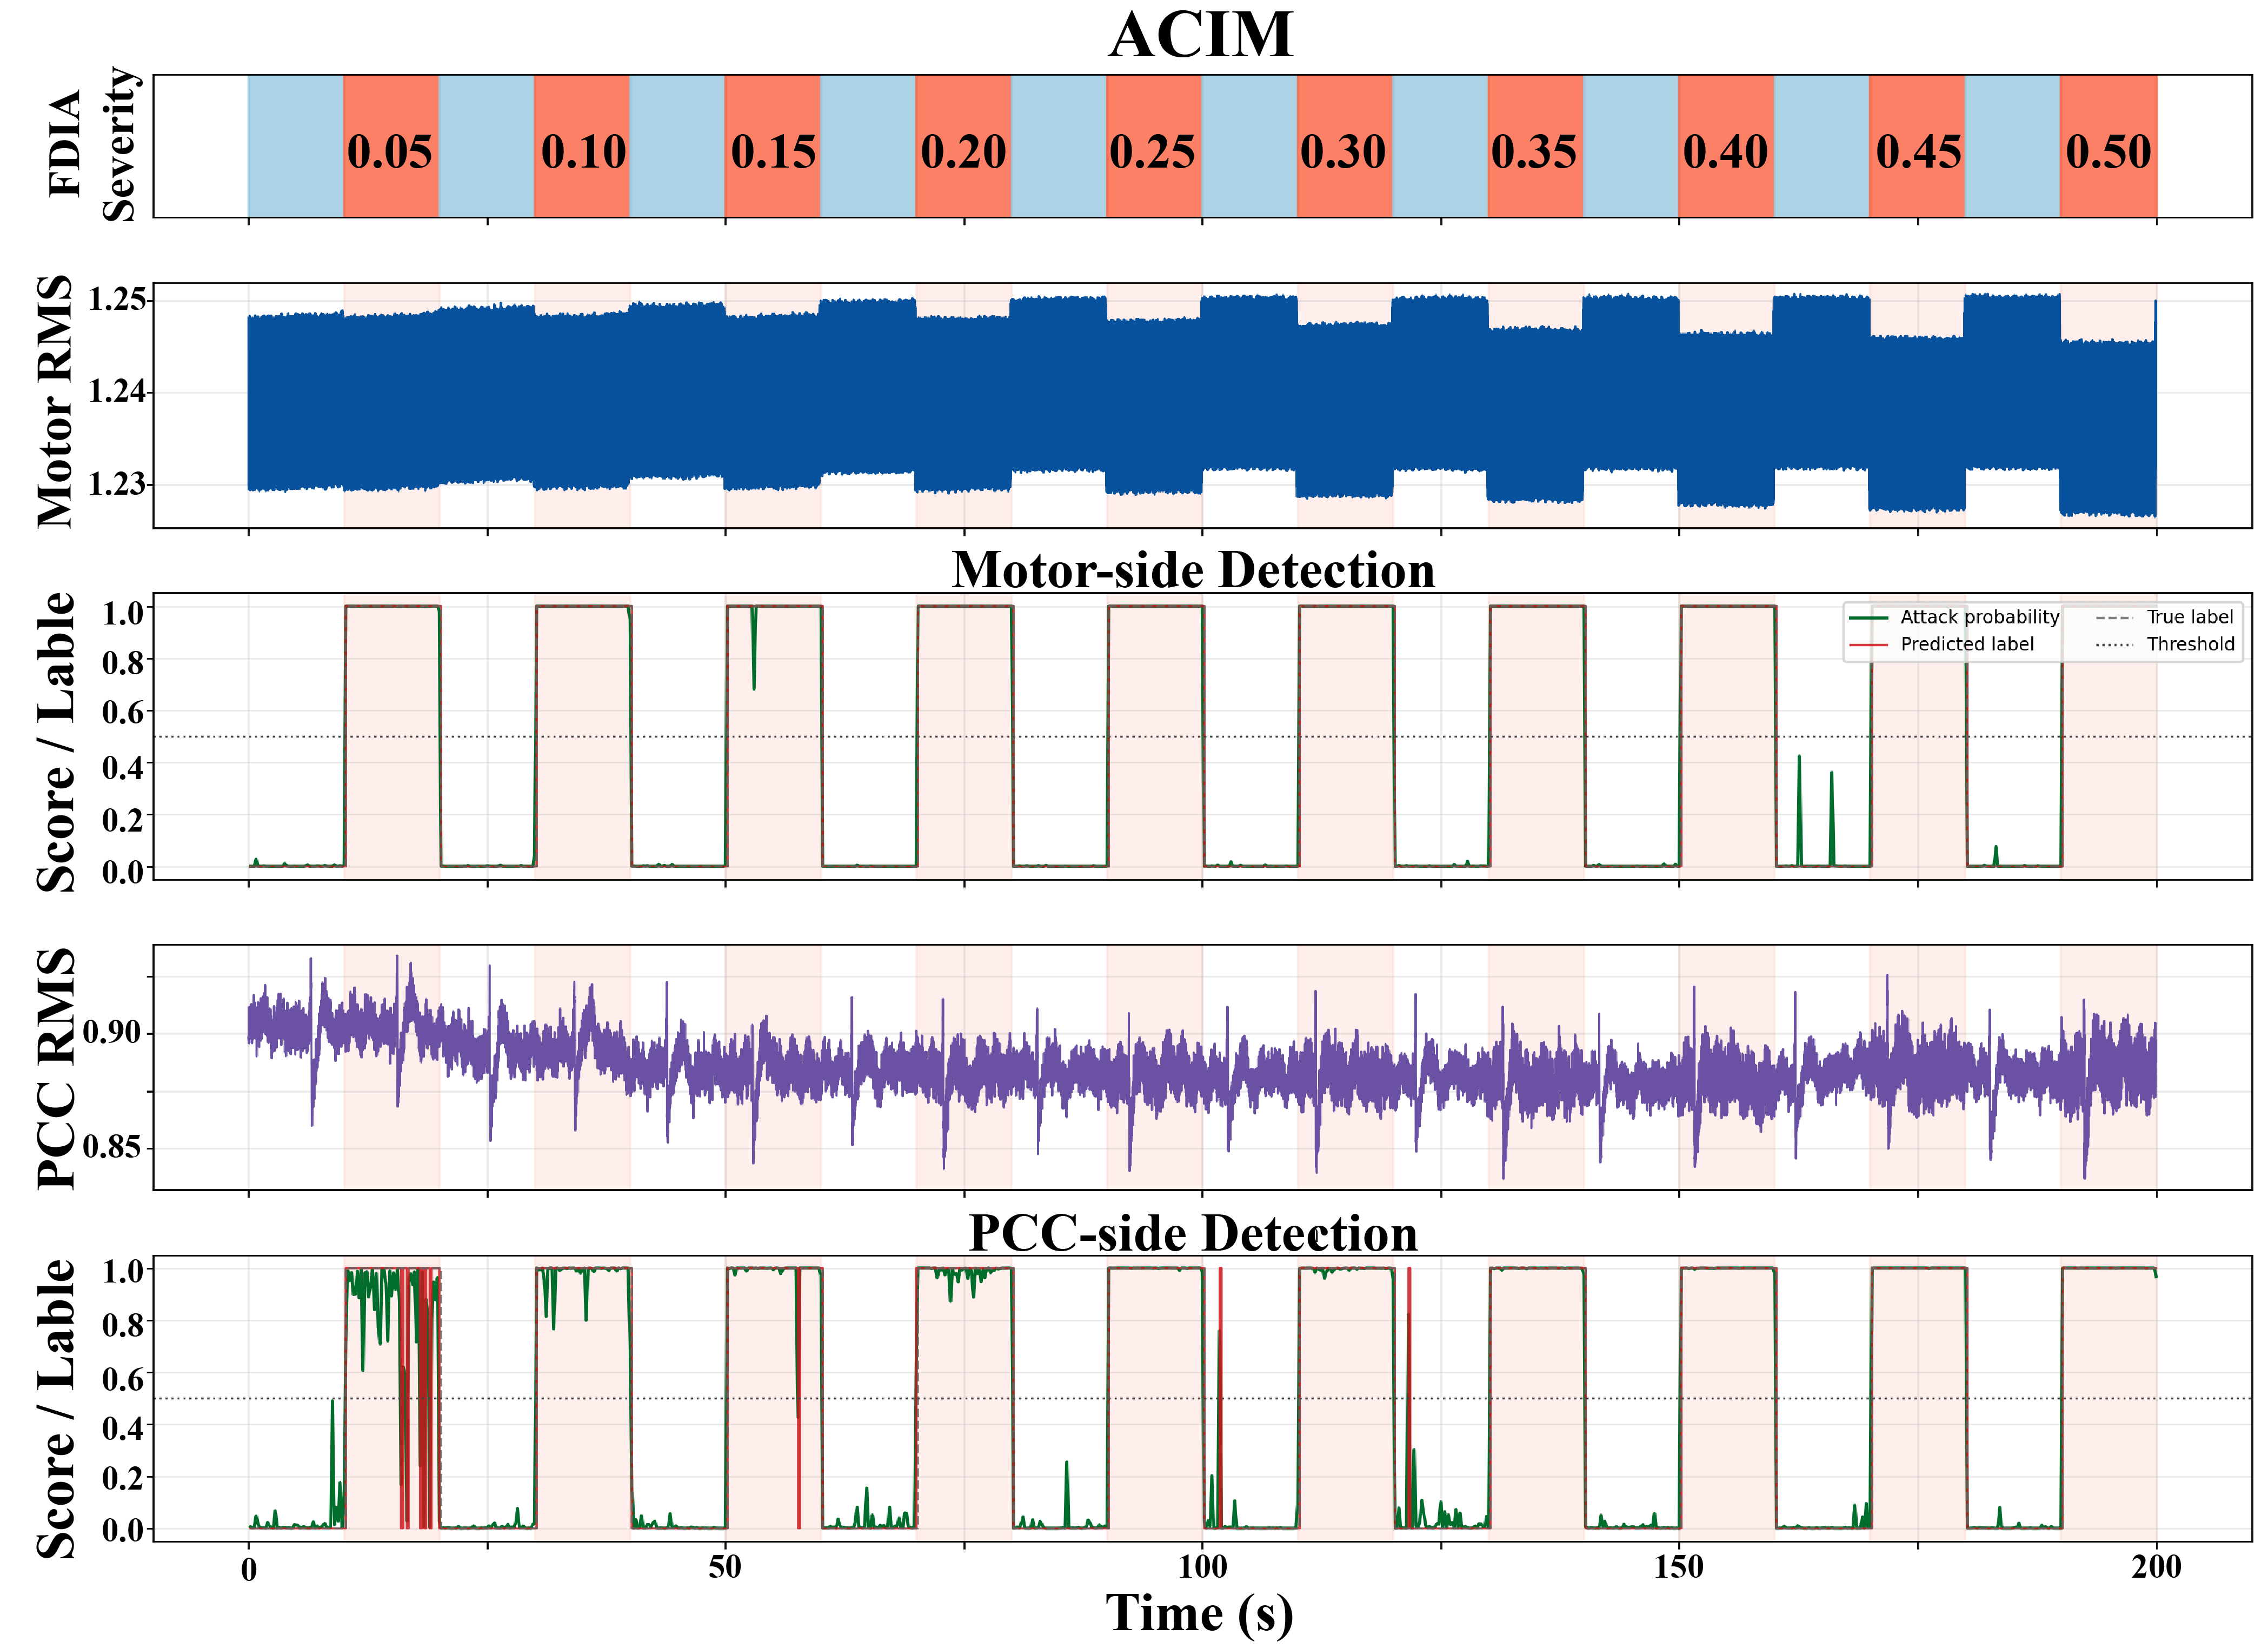
\includegraphics[width=0.98\columnwidth]{figs/case1_30_motor_pcc_model_detection_200s_0p2s_rms61_continuous_revised.png}
    {}
    \vspace{0.3em}
    \textbf{(a)} 200 s overview

    \vspace{0.8em}

    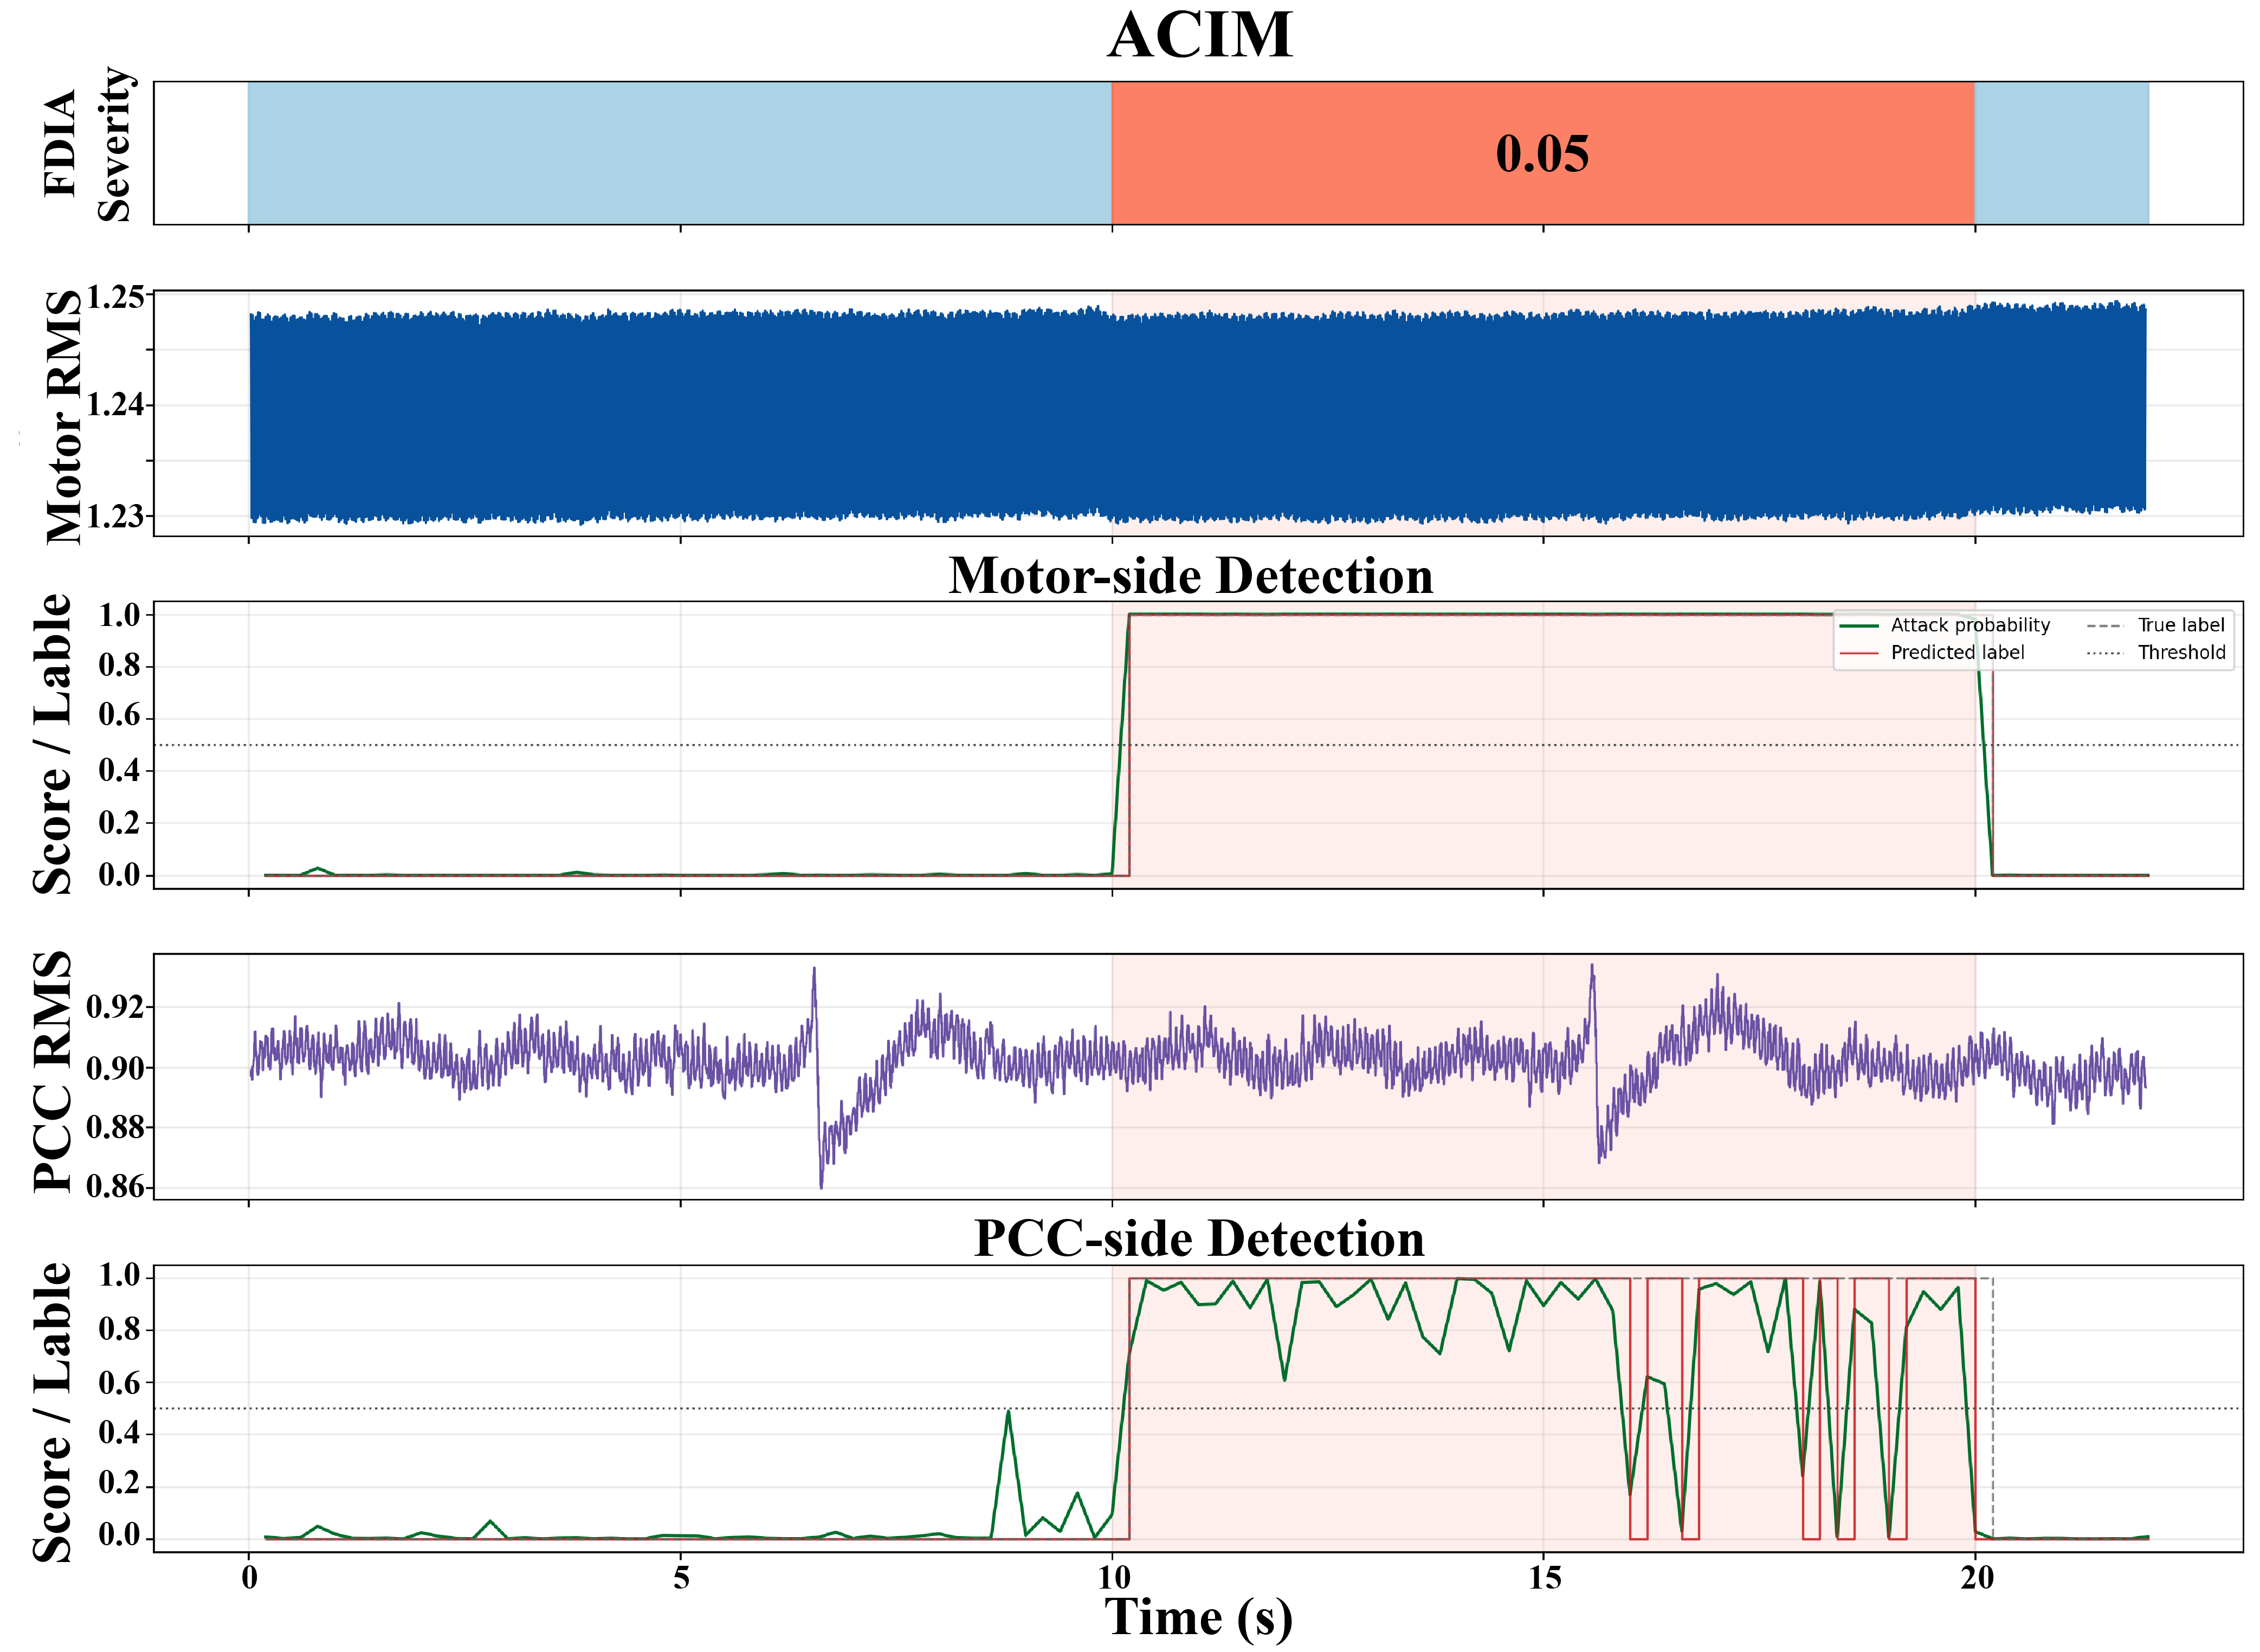
\includegraphics[width=0.98\columnwidth]{figs/case1_30_motor_pcc_model_detection_0_22s_0p2s_rms61_continuous_revised.png}

    \vspace{0.3em}
    \textbf{(b)} 0--22 s zoomed view
    \DiffOriginalCaption{Figure 6: Representative continuous-signal FDIA detection example for the ACIM. Panel (a) shows the 200-s sequence, and panel (b) zooms into the minor attack transition.}


\end{minipage}\par\vspace{1em}
% Complete new block: fig:case1_30_motor_pcc_detection_examples
\begin{minipage}[t]{\DiffColumnWidth}
\centering
\textcolor{blue}{\textbf{REVISED --- Figure 7 (main\_revised.tex)}}\par\smallskip

\centering
\begingroup\setlength{\unitlength}{1bp}
\resizebox{0.98\linewidth}{!}{\begin{picture}(252,402)
\put(151.0000,395.0000){\makebox(0,0){\color{black}\fontsize{9bp}{10bp}\selectfont (a) 200-s overview}}
\put(54.0000,372){\color[rgb]{0.665,0.809,0.887}\rule{9.7000bp}{8bp}}
\put(63.7000,372){\color[rgb]{0.986,0.489,0.375}\rule{9.7000bp}{8bp}}
\put(68.5500,385.0000){\makebox(0,0){\color{black}\fontsize{7.5bp}{8.5bp}\selectfont 0.05}}
\put(73.4000,372){\color[rgb]{0.665,0.809,0.887}\rule{9.7000bp}{8bp}}
\put(83.1000,372){\color[rgb]{0.986,0.489,0.375}\rule{9.7000bp}{8bp}}
\put(87.9500,385.0000){\makebox(0,0){\color{black}\fontsize{7.5bp}{8.5bp}\selectfont 0.10}}
\put(92.8000,372){\color[rgb]{0.665,0.809,0.887}\rule{9.7000bp}{8bp}}
\put(102.5000,372){\color[rgb]{0.986,0.489,0.375}\rule{9.7000bp}{8bp}}
\put(107.3500,385.0000){\makebox(0,0){\color{black}\fontsize{7.5bp}{8.5bp}\selectfont 0.15}}
\put(112.2000,372){\color[rgb]{0.665,0.809,0.887}\rule{9.7000bp}{8bp}}
\put(121.9000,372){\color[rgb]{0.986,0.489,0.375}\rule{9.7000bp}{8bp}}
\put(126.7500,385.0000){\makebox(0,0){\color{black}\fontsize{7.5bp}{8.5bp}\selectfont 0.20}}
\put(131.6000,372){\color[rgb]{0.665,0.809,0.887}\rule{9.7000bp}{8bp}}
\put(141.3000,372){\color[rgb]{0.986,0.489,0.375}\rule{9.7000bp}{8bp}}
\put(146.1500,385.0000){\makebox(0,0){\color{black}\fontsize{7.5bp}{8.5bp}\selectfont 0.25}}
\put(151.0000,372){\color[rgb]{0.665,0.809,0.887}\rule{9.7000bp}{8bp}}
\put(160.7000,372){\color[rgb]{0.986,0.489,0.375}\rule{9.7000bp}{8bp}}
\put(165.5500,385.0000){\makebox(0,0){\color{black}\fontsize{7.5bp}{8.5bp}\selectfont 0.30}}
\put(170.4000,372){\color[rgb]{0.665,0.809,0.887}\rule{9.7000bp}{8bp}}
\put(180.1000,372){\color[rgb]{0.986,0.489,0.375}\rule{9.7000bp}{8bp}}
\put(184.9500,385.0000){\makebox(0,0){\color{black}\fontsize{7.5bp}{8.5bp}\selectfont 0.35}}
\put(189.8000,372){\color[rgb]{0.665,0.809,0.887}\rule{9.7000bp}{8bp}}
\put(199.5000,372){\color[rgb]{0.986,0.489,0.375}\rule{9.7000bp}{8bp}}
\put(204.3500,385.0000){\makebox(0,0){\color{black}\fontsize{7.5bp}{8.5bp}\selectfont 0.40}}
\put(209.2000,372){\color[rgb]{0.665,0.809,0.887}\rule{9.7000bp}{8bp}}
\put(218.9000,372){\color[rgb]{0.986,0.489,0.375}\rule{9.7000bp}{8bp}}
\put(223.7500,385.0000){\makebox(0,0){\color{black}\fontsize{7.5bp}{8.5bp}\selectfont 0.45}}
\put(228.6000,372){\color[rgb]{0.665,0.809,0.887}\rule{9.7000bp}{8bp}}
\put(238.3000,372){\color[rgb]{0.986,0.489,0.375}\rule{9.7000bp}{8bp}}
\put(243.1500,385.0000){\makebox(0,0){\color{black}\fontsize{7.5bp}{8.5bp}\selectfont 0.50}}
\put(26.0000,376.0000){\makebox(0,0){\color{black}\fontsize{8bp}{9bp}\selectfont Bias (\%)}}
\put(54,335){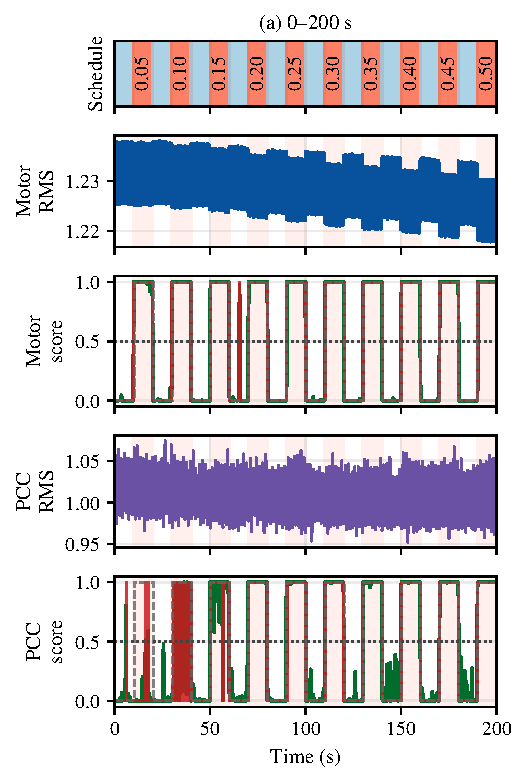
\includegraphics[viewport=55.00187500 255.79903999 238.37500000 309.43998591,clip,width=194bp,height=28bp]{figs_revised/figure6_overview_original_style.pdf}}
\put(54,335){\color{black}\linethickness{0.35bp}\framebox(194,28){}}
\put(12.0000,349.0000){\makebox(0,0){\color{black}\fontsize{8bp}{9bp}\selectfont \shortstack{Motor\\RMS}}}
\put(50.0000,339.0381){\makebox(0,0)[r]{\color{black}\fontsize{8bp}{9bp}\selectfont 1.22}}
\put(50.0000,351.4920){\makebox(0,0)[r]{\color{black}\fontsize{8bp}{9bp}\selectfont 1.23}}
\put(54,298){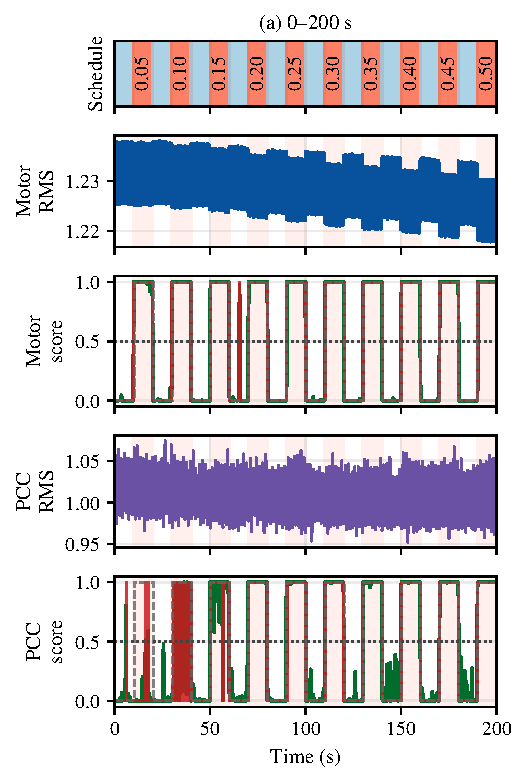
\includegraphics[viewport=55.00187500 179.27659911 238.37500000 241.85770268,clip,width=194bp,height=28bp]{figs_revised/figure6_overview_original_style.pdf}}
\put(54,298){\color{black}\linethickness{0.35bp}\framebox(194,28){}}
\put(12.0000,312.0000){\makebox(0,0){\color{black}\fontsize{8bp}{9bp}\selectfont \shortstack{Motor\\score}}}
\put(50.0000,299.2727){\makebox(0,0)[r]{\color{black}\fontsize{8bp}{9bp}\selectfont 0.0}}
\put(50.0000,312.0000){\makebox(0,0)[r]{\color{black}\fontsize{8bp}{9bp}\selectfont 0.5}}
\put(50.0000,324.7273){\makebox(0,0)[r]{\color{black}\fontsize{8bp}{9bp}\selectfont 1.0}}
\put(54,261){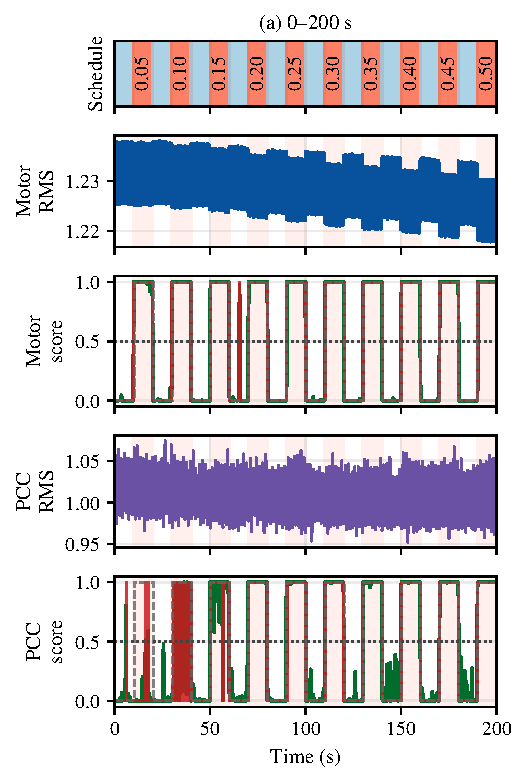
\includegraphics[viewport=55.00187500 111.69431588 238.37500000 165.33526180,clip,width=194bp,height=28bp]{figs_revised/figure6_overview_original_style.pdf}}
\put(54,261){\color{black}\linethickness{0.35bp}\framebox(194,28){}}
\put(12.0000,275.0000){\makebox(0,0){\color{black}\fontsize{8bp}{9bp}\selectfont \shortstack{PCC\\RMS}}}
\put(50.0000,261.8090){\makebox(0,0)[r]{\color{black}\fontsize{8bp}{9bp}\selectfont 0.95}}
\put(50.0000,272.2451){\makebox(0,0)[r]{\color{black}\fontsize{8bp}{9bp}\selectfont 1.00}}
\put(50.0000,282.6812){\makebox(0,0)[r]{\color{black}\fontsize{8bp}{9bp}\selectfont 1.05}}
\put(54,224){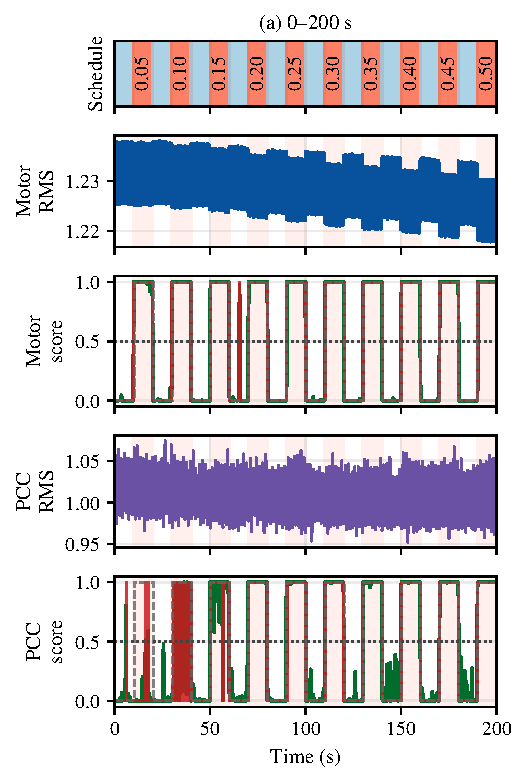
\includegraphics[viewport=55.00187500 35.17187500 238.37500000 97.75297858,clip,width=194bp,height=28bp]{figs_revised/figure6_overview_original_style.pdf}}
\put(54,224){\color{black}\linethickness{0.35bp}\framebox(194,28){}}
\put(12.0000,238.0000){\makebox(0,0){\color{black}\fontsize{8bp}{9bp}\selectfont \shortstack{PCC\\score}}}
\put(50.0000,225.2727){\makebox(0,0)[r]{\color{black}\fontsize{8bp}{9bp}\selectfont 0.0}}
\put(50.0000,238.0000){\makebox(0,0)[r]{\color{black}\fontsize{8bp}{9bp}\selectfont 0.5}}
\put(50.0000,250.7273){\makebox(0,0)[r]{\color{black}\fontsize{8bp}{9bp}\selectfont 1.0}}
\put(54.0000,217.0000){\makebox(0,0){\color{black}\fontsize{8bp}{9bp}\selectfont 0}}
\put(102.5000,217.0000){\makebox(0,0){\color{black}\fontsize{8bp}{9bp}\selectfont 50}}
\put(151.0000,217.0000){\makebox(0,0){\color{black}\fontsize{8bp}{9bp}\selectfont 100}}
\put(199.5000,217.0000){\makebox(0,0){\color{black}\fontsize{8bp}{9bp}\selectfont 150}}
\put(248.0000,217.0000){\makebox(0,0){\color{black}\fontsize{8bp}{9bp}\selectfont 200}}
\put(151.0000,207.0000){\makebox(0,0){\color{black}\fontsize{8bp}{9bp}\selectfont Time (s)}}
\put(151.0000,190.0000){\makebox(0,0){\color{black}\fontsize{9bp}{10bp}\selectfont (b) 0--22-s detail}}
\put(54.0000,167){\color[rgb]{0.665,0.809,0.887}\rule{88.1818bp}{8bp}}
\put(142.1818,167){\color[rgb]{0.986,0.489,0.375}\rule{88.1818bp}{8bp}}
\put(186.2727,180.0000){\makebox(0,0){\color{black}\fontsize{7.5bp}{8.5bp}\selectfont 0.05}}
\put(230.3636,167){\color[rgb]{0.665,0.809,0.887}\rule{17.6364bp}{8bp}}
\put(26.0000,171.0000){\makebox(0,0){\color{black}\fontsize{8bp}{9bp}\selectfont Bias (\%)}}
\put(54,130){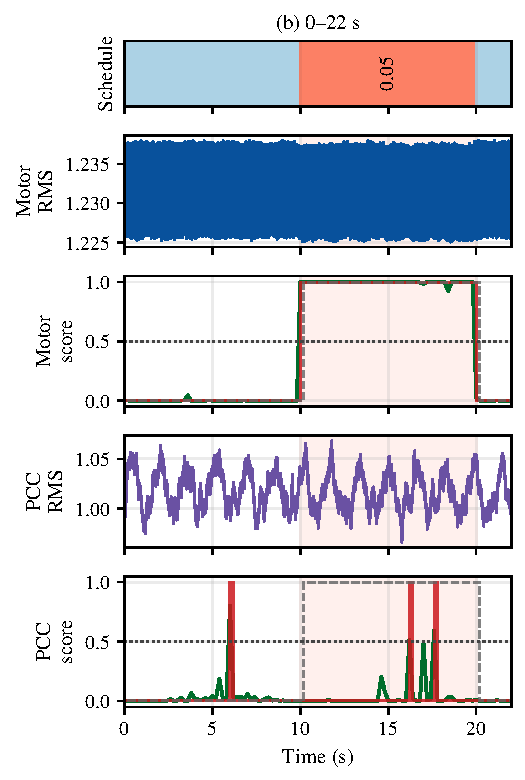
\includegraphics[viewport=59.72687500 255.79903999 245.50000000 309.43998591,clip,width=194bp,height=28bp]{figs_revised/figure6_zoom_original_style.pdf}}
\put(54,130){\color{black}\linethickness{0.35bp}\framebox(194,28){}}
\put(12.0000,144.0000){\makebox(0,0){\color{black}\fontsize{8bp}{9bp}\selectfont \shortstack{Motor\\RMS}}}
\put(50.0000,131.1569){\makebox(0,0)[r]{\color{black}\fontsize{8bp}{9bp}\selectfont 1.225}}
\put(50.0000,141.0041){\makebox(0,0)[r]{\color{black}\fontsize{8bp}{9bp}\selectfont 1.230}}
\put(50.0000,150.8513){\makebox(0,0)[r]{\color{black}\fontsize{8bp}{9bp}\selectfont 1.235}}
\put(54,93){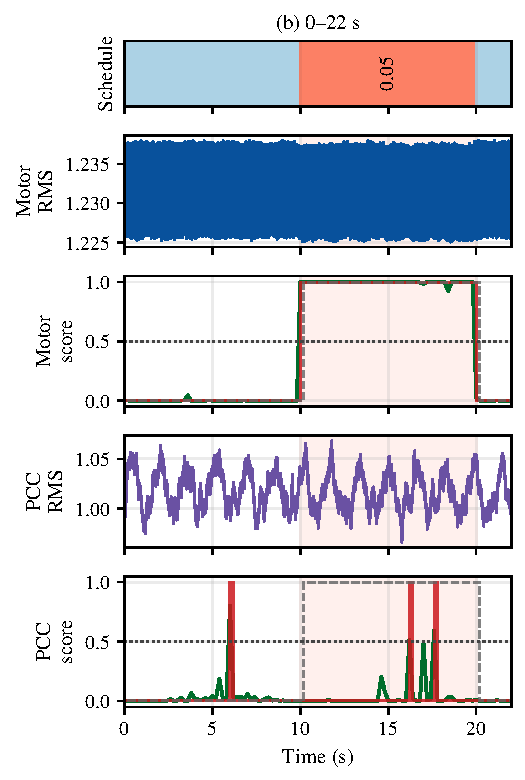
\includegraphics[viewport=59.72687500 179.27659911 245.50000000 241.85770268,clip,width=194bp,height=28bp]{figs_revised/figure6_zoom_original_style.pdf}}
\put(54,93){\color{black}\linethickness{0.35bp}\framebox(194,28){}}
\put(12.0000,107.0000){\makebox(0,0){\color{black}\fontsize{8bp}{9bp}\selectfont \shortstack{Motor\\score}}}
\put(50.0000,94.2727){\makebox(0,0)[r]{\color{black}\fontsize{8bp}{9bp}\selectfont 0.0}}
\put(50.0000,107.0000){\makebox(0,0)[r]{\color{black}\fontsize{8bp}{9bp}\selectfont 0.5}}
\put(50.0000,119.7273){\makebox(0,0)[r]{\color{black}\fontsize{8bp}{9bp}\selectfont 1.0}}
\put(54,56){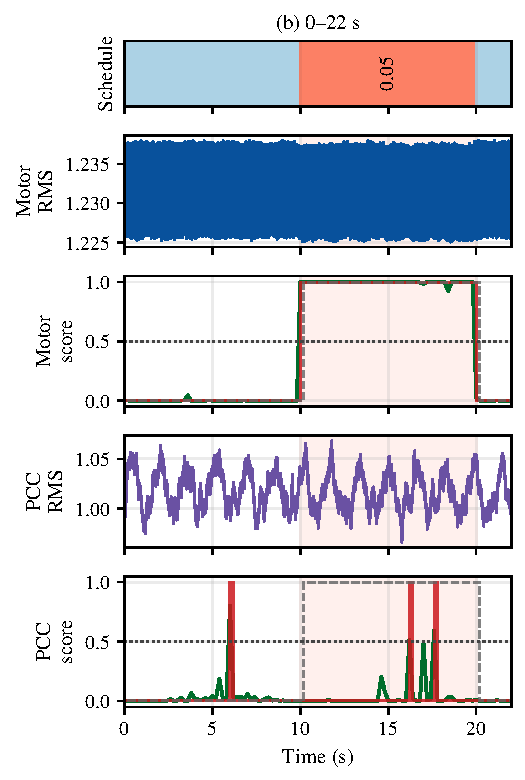
\includegraphics[viewport=59.72687500 111.69431588 245.50000000 165.33526180,clip,width=194bp,height=28bp]{figs_revised/figure6_zoom_original_style.pdf}}
\put(54,56){\color{black}\linethickness{0.35bp}\framebox(194,28){}}
\put(12.0000,70.0000){\makebox(0,0){\color{black}\fontsize{8bp}{9bp}\selectfont \shortstack{PCC\\RMS}}}
\put(50.0000,65.7333){\makebox(0,0)[r]{\color{black}\fontsize{8bp}{9bp}\selectfont 1.00}}
\put(50.0000,78.1919){\makebox(0,0)[r]{\color{black}\fontsize{8bp}{9bp}\selectfont 1.05}}
\put(54,19){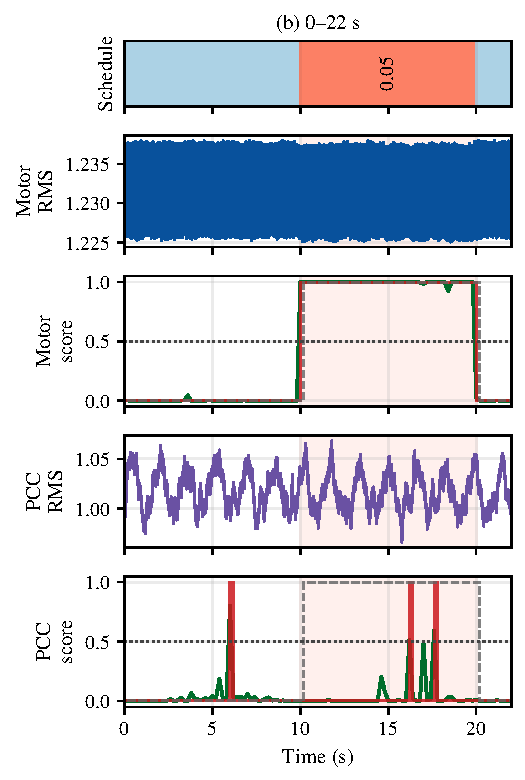
\includegraphics[viewport=59.72687500 35.17187500 245.50000000 97.75297858,clip,width=194bp,height=28bp]{figs_revised/figure6_zoom_original_style.pdf}}
\put(54,19){\color{black}\linethickness{0.35bp}\framebox(194,28){}}
\put(12.0000,33.0000){\makebox(0,0){\color{black}\fontsize{8bp}{9bp}\selectfont \shortstack{PCC\\score}}}
\put(50.0000,20.2727){\makebox(0,0)[r]{\color{black}\fontsize{8bp}{9bp}\selectfont 0.0}}
\put(50.0000,33.0000){\makebox(0,0)[r]{\color{black}\fontsize{8bp}{9bp}\selectfont 0.5}}
\put(50.0000,45.7273){\makebox(0,0)[r]{\color{black}\fontsize{8bp}{9bp}\selectfont 1.0}}
\put(54.0000,12.0000){\makebox(0,0){\color{black}\fontsize{8bp}{9bp}\selectfont 0}}
\put(98.0909,12.0000){\makebox(0,0){\color{black}\fontsize{8bp}{9bp}\selectfont 5}}
\put(142.1818,12.0000){\makebox(0,0){\color{black}\fontsize{8bp}{9bp}\selectfont 10}}
\put(186.2727,12.0000){\makebox(0,0){\color{black}\fontsize{8bp}{9bp}\selectfont 15}}
\put(230.3636,12.0000){\makebox(0,0){\color{black}\fontsize{8bp}{9bp}\selectfont 20}}
\put(151.0000,2.0000){\makebox(0,0){\color{black}\fontsize{8bp}{9bp}\selectfont Time (s)}}
\end{picture}}
\endgroup
\caption{Held-out ACIM detection: (a) 200-s overview and (b) 22-s detail of the first attack onset. Shading denotes attack intervals.}
\label{fig:case1_30_motor_pcc_detection_examples}

\end{minipage}
\end{minipage}
\end{adjustbox}
\end{figure*}




\DIFaddend \section{LATENCY AND REDUCED-FEATURE INFERENCE ANALYSIS}
\label{sec:realtime}
\DIFaddbegin

\DIFaddend Practical PCC monitoring requires low latency and stable online throughput. This section reports per-window latency, throughput, pruning, and reduced-feature effects.
\DIFdelbegin \DIFdel{In particular, the analysis focuses on end-to-end processing latency, online throughput, feature-pruning effects, and practical considerations for deployment at the PCC.
}\DIFdelend

\subsection{Inference Latency and Throughput on CPU/GPU}
\label{sec:latency_throughput}
\DIFaddbegin

\DIFaddend Runtime was benchmarked on an Intel Core Ultra 9 285K CPU and NVIDIA RTX 5090 GPU using the selected \DIFaddbegin \DIFadd{seed-1234 }\DIFaddend LF/HF-Inception \DIFaddbegin \DIFadd{binary }\DIFaddend pipelines. The benchmark was split into three stages: (i) LF/HF feature extraction from one 2{,}000-sample raw window, (ii) \DIFaddbegin \DIFadd{normalization, host-to-device transfer, and }\DIFaddend model inference on the resulting feature tensor, and (iii) end-to-end per-window execution. \DIFdelbegin \DIFdel{GPU inference was measured with and without host-to-device transfer}\DIFdelend \DIFaddbegin \DIFadd{Each variant used 10 warm-up runs and 50 timed repetitions, with randomized variant order. Processing starts from an available measurement window; acquisition and disk I/O are excluded}\DIFaddend .

Table~\ref{tab:runtime_latency} summarizes the measured per-window latencies. For the PCC stream, LF/HF feature extraction required \DIFdelbegin \DIFdel{21.72}\DIFdelend \DIFaddbegin \DIFadd{22.30}\DIFaddend ~ms on CPU\DIFdelbegin \DIFdel{and the Inception model needs only 0.71~ms on GPU. When host-to-device transferwas included, the GPU inference stage remained sub-millisecond at 0.74}\DIFdelend \DIFaddbegin \DIFadd{, while normalization, transfer, and GPU inference required 0.78}\DIFaddend ~ms. As a result, the \DIFaddbegin \DIFadd{median }\DIFaddend PCC end-to-end \DIFdelbegin \DIFdel{latency was only 22.46~msfor End-to-End inference}\DIFdelend \DIFaddbegin \DIFadd{processing latency was 23.03~ms}\DIFaddend .
A similar pattern was observed for the motor stream. Feature extraction required \DIFdelbegin \DIFdel{65.25}\DIFdelend \DIFaddbegin \DIFadd{66.38}\DIFaddend ~ms on CPU, while \DIFdelbegin \DIFdel{model inference required 0.36~ms on GPU. Including transfer, the GPU inference stage was 0.38}\DIFdelend \DIFaddbegin \DIFadd{normalization, transfer, and GPU inference required 1.42}\DIFaddend ~ms, leading to \DIFdelbegin \DIFdel{an }\DIFdelend \DIFaddbegin \DIFadd{a median }\DIFaddend end-to-end latency of \DIFdelbegin \DIFdel{65.63}\DIFdelend \DIFaddbegin \DIFadd{67.81}\DIFaddend ~ms. \DIFdelbegin \DIFdel{For the tested PCC pipeline, the measured end-to-end latency was 22.46 ms under the reported hardware configuration. }\DIFdelend In terms of throughput, the end-to-end PCC pipeline \DIFdelbegin \DIFdel{sustained 44.53 }\DIFdelend \DIFaddbegin \DIFadd{had a reciprocal-median processing rate of 43.42 }\DIFaddend windows/s, while the corresponding motor pipeline sustained \DIFdelbegin \DIFdel{15.24 }\DIFdelend \DIFaddbegin \DIFadd{14.75 }\DIFaddend windows/s.



\DIFaddbegin \begin{table*}[p]
\centering
\begin{adjustbox}{max width=\textwidth,max totalheight=0.87\textheight}
\begin{minipage}{\textwidth}
\centering
% Complete old block: tab:runtime_latency
\begin{minipage}[t]{0.48\textwidth}
\centering
\textcolor{red}{\textbf{ORIGINAL --- Table 9 (main.tex)}}\par\smallskip

\centering
\scriptsize
\DiffOriginalCaption{Table 9: Measured per-window latency and throughput of the GPU-assisted LF/HF-InceptionTime pipeline.}

\renewcommand{\arraystretch}{1.15}
\setlength{\tabcolsep}{3pt}
\begin{adjustbox}{max width=\linewidth}\begin{tabular}{l c c c c c}
\hline
Stream & Feature & GPU Inference & GPU Transfer + & End-to-End & Throughput \\
 & Extraction (ms) & (ms) & Inference (ms) & (ms) & (windows/s) \\
\hline
PCC   & 21.72 & 0.71 & 0.74 & 22.46 & 44.53 \\
Motor & 65.25 & 0.36 & 0.38 & 65.63 & 15.24 \\
\hline
\end{tabular}\end{adjustbox}

\end{minipage}\hfill%
% Complete new block: tab:runtime_latency
\begin{minipage}[t]{0.48\textwidth}
\centering
\textcolor{blue}{\textbf{REVISED --- Table 9 (main\_revised.tex)}}\par\smallskip

\centering
\footnotesize
\caption{GPU-assisted per-window latency and processing rate.}
\label{tab:runtime_latency}
\renewcommand{\arraystretch}{1.15}
\setlength{\tabcolsep}{2pt}
\begin{tabular}{@{}lcccc@{}}
\hline
Statistic & \shortstack{Feature\\extract.\\(ms)} & \shortstack{Norm./transfer\\+ inference\\(ms)} & \shortstack{Total\\processing\\(ms)} & \shortstack{Rate\\(windows/s)} \\\hline
\hline\multicolumn{5}{c}{\textit{PCC stream}} \\\hline
Median & 22.30 & 0.78 & 23.03 & 43.42 \\
95th pct. & 24.15 & 0.95 & 25.03 & -- \\
\hline\multicolumn{5}{c}{\textit{MOTOR stream}} \\\hline
Median & 66.38 & 1.42 & 67.81 & 14.75 \\
95th pct. & 75.52 & 1.58 & 76.98 & -- \\
\hline\end{tabular}
\par\smallskip\begin{minipage}{\columnwidth}\scriptsize Rate is the reciprocal of median total processing time. Stages are timed within each iteration; marginal percentiles need not sum. Acquisition and disk I/O are excluded.\end{minipage}

\end{minipage}
\end{minipage}
\end{adjustbox}
\end{table*}




\DIFaddend \subsection{Feature Pruning for Low-Latency Anomaly Detection}
\DIFdelbegin %DIFDELCMD < \label{sec:latency_throughput}
%DIFDELCMD < %%%
\DIFdelend \DIFaddbegin \label{sec:feature_pruning}

\DIFaddend Feature pruning was evaluated for the \texttt{fdia2} task to reduce online latency. Features were ranked by permutation importance, defined as the \DIFaddbegin \DIFadd{validation }\DIFaddend balanced-accuracy drop caused by permuting each feature \DIFdelbegin \DIFdel{column}\DIFdelend \DIFaddbegin \DIFadd{trajectory across windows, averaged over three permutations. Test labels were not used for ranking}\DIFaddend . Reduced subsets were then formed using global top-\(75\%\), top-\(50\%\), and top-\(25\%\) rankings, as well as per-channel top-15 and top-10 selections. Because the benchmark uses selective LF/HF feature computation, only retained features \DIFdelbegin \DIFdel{are extracted}\DIFdelend \DIFaddbegin \DIFadd{and their required intermediate quantities are calculated}\DIFaddend ; therefore, the measured extraction latency reflects the computational benefit of pruning. \DIFaddbegin \DIFadd{Each reduced subset was retrained using the full model's selected architecture and training protocol.
}\DIFaddend


Table~\ref{tab:feature_pruning_anomaly2_runtime} shows that pruning can reduce latency while preserving, and in some cases improving, detection performance. For the PCC stream, \DIFdelbegin \DIFdel{the best tradeoff }\DIFdelend \DIFaddbegin \DIFadd{a compact representation }\DIFaddend was obtained with the top-\(25\%\) subset, which retained 18 of 74 features. This subset \DIFdelbegin \DIFdel{improved balanced accuracy from 88.99\% to 90.11}\DIFdelend \DIFaddbegin \DIFadd{retained the full model's mean balanced accuracy of 80.29}\DIFaddend \% and reduced end-to-end CPU+GPU latency from \DIFdelbegin \DIFdel{25.38}\DIFdelend \DIFaddbegin \DIFadd{23.03}\DIFaddend ~ms to \DIFdelbegin \DIFdel{19.71}\DIFdelend \DIFaddbegin \DIFadd{12.44}\DIFaddend ~ms, corresponding to \DIFdelbegin \DIFdel{a 1.29\(\times\) }\DIFdelend \DIFaddbegin \DIFadd{an 85.18\% }\DIFaddend speedup. For the motor stream, the top-\(25\%\) subset retained 56 of 222 features, \DIFdelbegin \DIFdel{improved }\DIFdelend \DIFaddbegin \DIFadd{reduced }\DIFaddend balanced accuracy from \DIFdelbegin \DIFdel{98.85\% to 99.48}\DIFdelend \DIFaddbegin \DIFadd{88.26\% to 86.83}\DIFaddend \%, and reduced latency from \DIFdelbegin \DIFdel{109.07}\DIFdelend \DIFaddbegin \DIFadd{67.81}\DIFaddend ~ms to \DIFdelbegin \DIFdel{56.21}\DIFdelend \DIFaddbegin \DIFadd{27.87}\DIFaddend ~ms, corresponding to a \DIFdelbegin \DIFdel{1.94\(\times\) }\DIFdelend \DIFaddbegin \DIFadd{143.33\% }\DIFaddend speedup.

\DIFdelbegin \DIFdel{The intermediate subsets did not always reduce runtime, even when they contained fewer features}\DIFdelend \DIFaddbegin \DIFadd{All evaluated subsets reduced runtime, but the reduction was not proportional to feature count}\DIFaddend . This indicates that pruning effectiveness depends not only on feature count, but also on which LF, HF, and TD \DIFdelbegin \DIFdel{feature families remain active}\DIFdelend \DIFaddbegin \DIFadd{calculations remain necessary}\DIFaddend . The feature-importance rankings in Fig.~\ref{fig:top10_feature_importance} further show that the two sensing streams rely on different features: motor-side detection is dominated by TD and selected LF features, whereas PCC-side detection places greater emphasis on harmonic and waveform-shape features. \DIFdelbegin %DIFDELCMD <

%DIFDELCMD < %%%
\DIFdel{Overall, the LF}\DIFdelend \DIFaddbegin \DIFadd{Bars show mean validation importance and whiskers show one standard deviation across three holdouts. Motor channels 1--3}\DIFaddend /\DIFdelbegin \DIFdel{HF representation contains redundancy for anomaly detection, and structured pruning can improve both latency and predictive performance. This is especially relevant for PCC-based monitoring, where the compact top-\(25\%\) subset provides both the fastest and most accurate PCC detector}\DIFdelend \DIFaddbegin \DIFadd{4--6 are ACIM/PMSM currents; PCC channels 1/2 are voltage/current}\DIFaddend .






\DIFaddbegin \begin{figure*}[p]
\centering
\begin{adjustbox}{max width=\textwidth,max totalheight=0.87\textheight}
\begin{minipage}{\textwidth}
\centering
% Complete old block: fig:top10_feature_importance
\begin{minipage}[t]{\textwidth}
\centering
\textcolor{red}{\textbf{ORIGINAL --- Figure 7 (main.tex)}}\par\smallskip

    \centering
    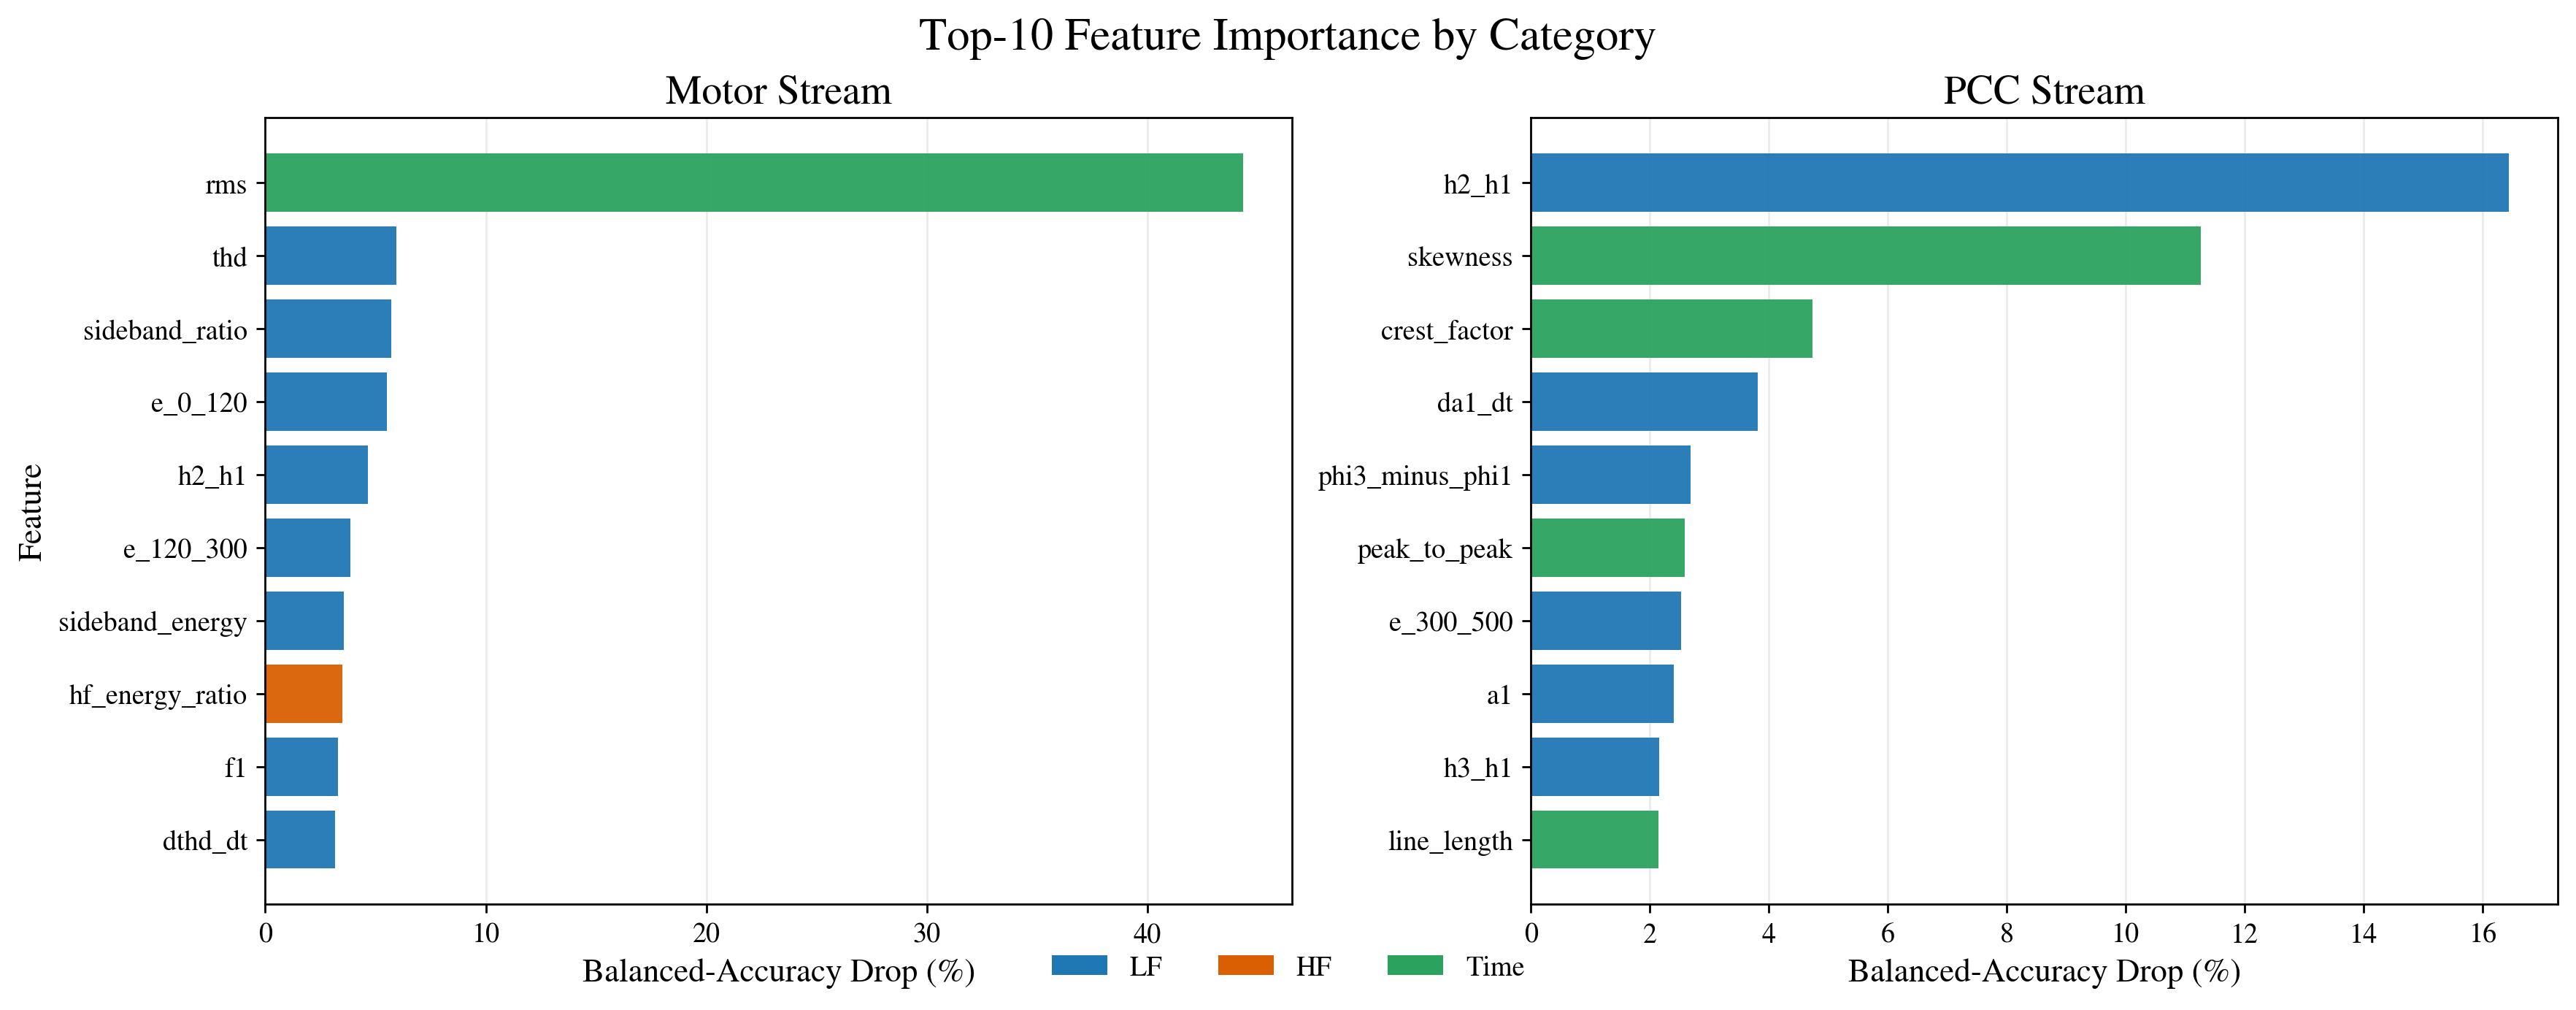
\includegraphics[width=0.95\textwidth]{figs/top10_feature_importance_motor_pcc_typed_clean.png}
    \DiffOriginalCaption{Figure 7: Feature-importance rankings for the motor and PCC streams.}


\end{minipage}\par\vspace{1em}
% Complete new block: fig:top10_feature_importance
\begin{minipage}[t]{\textwidth}
\centering
\textcolor{blue}{\textbf{REVISED --- Figure 8 (main\_revised.tex)}}\par\smallskip

\centering
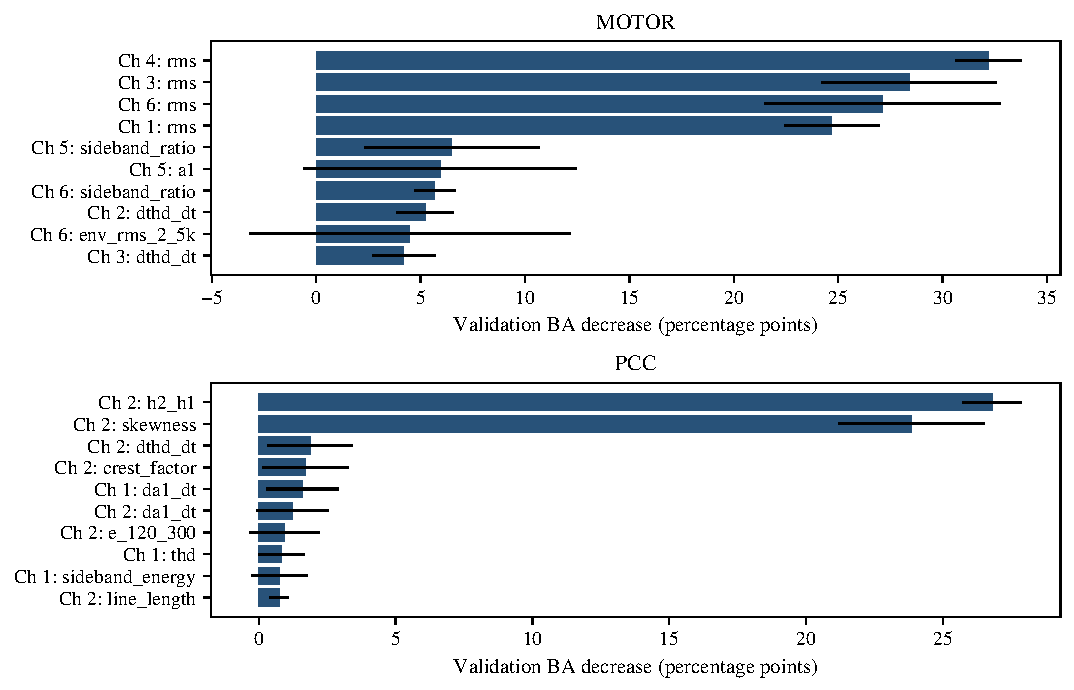
\includegraphics[width=\linewidth]{figs_revised/figure7_validation_feature_importance.pdf}
\caption{Top ten features by validation permutation importance for motor and PCC detection. Error bars show one standard deviation.}
\label{fig:top10_feature_importance}

\end{minipage}
\end{minipage}
\end{adjustbox}
\end{figure*}






\begin{table*}[p]
\centering
\begin{adjustbox}{max width=\textwidth,max totalheight=0.87\textheight}
\begin{minipage}{\textwidth}
\centering
% Complete old block: tab:feature_pruning_anomaly2_runtime
\begin{minipage}[t]{0.48\textwidth}
\centering
\textcolor{red}{\textbf{ORIGINAL --- Table 10 (main.tex)}}\par\smallskip

\centering
\scriptsize
\DiffOriginalCaption{Table 10: Effect of feature pruning on \texttt{fdia2} performance and runtime.}

\renewcommand{\arraystretch}{1.05}
\setlength{\tabcolsep}{2.5pt}
\begin{adjustbox}{max width=\linewidth}\begin{tabular}{l c c c c c c c}
\hline
Feature & No. & Balanced & F1 & Feature & End-to-End & Speedup & Runtime \\
Set & Feature & Accuracy (\%) & (\%) & Extraction (\%) & (ms) & ($\times$) & Gain(\%) \\
\hline
\multicolumn{7}{c}{\textit{PCC stream}} \\
\hline
Full   & 74  & 88.99 & 89.25 & 24.61 & 25.38  & 1.00 & 0 \\
75\%   & 56  & 88.65 & 88.88 & 22.11 & 22.91 & 1.11 & 11 \\
50\%   & 37  & 88.90 & 89.04 & 22.26 & 23.00 & 1.10 & 10 \\
25\%   & 18  & 90.11 & 90.28 & 18.88 & 19.71 & 1.29 & 29 \\
15/ch. & 30  & 89.33 & 89.52 & 33.95 & 34.70 & 0.73 & -27 \\
10/ch. & 20  & 89.40 & 89.61 & 19.09 & 20.23 & 1.25 & 25 \\
\hline
\multicolumn{7}{c}{\textit{Motor stream}} \\
\hline
Full   & 222 & 98.85 & 98.88 & 108.65 & 109.07 & 1.00 & 0 \\
75\%   & 166 & 99.24 & 99.27 & 110.15 & 110.74 & 0.98 & -2 \\
50\%   & 111 & 99.39 & 99.38 & 112.59 & 113.20 & 0.96 & -4 \\
25\%   & 56  & 99.48 & 99.51 & 55.84 & 56.21  & 1.94 & 94 \\
15/ch. & 90  & 99.49 & 99.50 & 104.02 & 104.60 & 1.04 & 4 \\
10/ch. & 60  & 99.46 & 99.47 & 62.19 & 62.79  & 1.74 & 74 \\
\hline
\end{tabular}\end{adjustbox}

\end{minipage}\hfill%
% Complete new block: tab:feature_pruning_anomaly2_runtime
\begin{minipage}[t]{0.48\textwidth}
\centering
\textcolor{blue}{\textbf{REVISED --- Table 10 (main\_revised.tex)}}\par\smallskip

\centering
\scriptsize
\caption{Feature pruning for \texttt{fdia2}: performance and runtime.}
\label{tab:feature_pruning_anomaly2_runtime}
\renewcommand{\arraystretch}{1.15}
\setlength{\tabcolsep}{1.7pt}
\begin{tabular}{@{}lcccccc@{}}
\hline
Subset & No. & \shortstack{BA\\(\%)} & \shortstack{F1\\(\%)} & \shortstack{Extract.\\(ms)} & \shortstack{Total\\(ms)} & \shortstack{Speedup\\(\%)} \\\hline
\hline\multicolumn{7}{c}{\textit{PCC stream}} \\\hline
Full & 74 & \mbox{80.29\,$\pm$\,3.03} & \mbox{80.42\,$\pm$\,2.96} & 22.30 & 23.03 & 0.00 \\
75\% & 56 & \mbox{78.28\,$\pm$\,3.07} & \mbox{78.41\,$\pm$\,3.37} & 19.65 & 20.33 & 13.26 \\
50\% & 37 & \mbox{78.87\,$\pm$\,2.79} & \mbox{79.10\,$\pm$\,2.97} & 16.63 & 17.31 & 33.07 \\
25\% & 18 & \mbox{80.29\,$\pm$\,2.14} & \mbox{80.58\,$\pm$\,2.29} & 11.81 & \textbf{12.44} & 85.18 \\
15/ch. & 30 & \mbox{77.59\,$\pm$\,4.75} & \mbox{77.74\,$\pm$\,4.94} & 15.64 & 16.25 & 41.76 \\
10/ch. & 20 & \mbox{\textbf{80.47}\,$\pm$\,2.79} & \mbox{\textbf{80.69}\,$\pm$\,2.80} & 12.07 & 12.68 & 81.60 \\
\hline\multicolumn{7}{c}{\textit{MOTOR stream}} \\\hline
Full & 222 & \mbox{88.26\,$\pm$\,9.99} & \mbox{87.23\,$\pm$\,11.39} & 66.38 & 67.81 & 0.00 \\
75\% & 166 & \mbox{87.95\,$\pm$\,11.38} & \mbox{87.19\,$\pm$\,12.42} & 56.28 & 57.70 & 17.52 \\
50\% & 111 & \mbox{89.28\,$\pm$\,11.33} & \mbox{88.20\,$\pm$\,12.87} & 45.50 & 46.89 & 44.62 \\
25\% & 56 & \mbox{86.83\,$\pm$\,10.93} & \mbox{85.44\,$\pm$\,12.39} & 26.57 & \textbf{27.87} & 143.33 \\
15/ch. & 90 & \mbox{\textbf{92.10}\,$\pm$\,9.71} & \mbox{\textbf{91.44}\,$\pm$\,10.88} & 37.68 & 38.96 & 74.04 \\
10/ch. & 60 & \mbox{88.18\,$\pm$\,9.28} & \mbox{87.20\,$\pm$\,10.62} & 28.48 & 29.80 & 127.56 \\
\hline\end{tabular}
\par\smallskip\begin{minipage}{\columnwidth}\scriptsize Performance: mean $\pm$ sample SD. Timing: seed-1234 GPU-assisted median; 95th percentiles are supplied in the results. Bold: highest BA/F1 or lowest total latency within a stream. Only selected statistics and their required intermediate calculations are evaluated. Percentage speedup is $100(T_{\mathrm{full}}/T_{\mathrm{subset}}-1)$, using median total processing times.\end{minipage}

\end{minipage}
\end{minipage}
\end{adjustbox}
\end{table*}




\DIFaddend \subsection{LF/HF/TD Ablation for Binary Anomaly Detection}
\label{sec:lfhf_ablation}
\DIFaddbegin

\DIFaddend A complementary LF/HF/TD ablation was performed on the \texttt{fdia2} task to identify which feature groups are most useful for binary anomaly detection in the PCC and motor streams. \DIFaddbegin \DIFadd{All seven combinations were retrained using the selected full-feature architecture within each stream and split. }\DIFaddend Detailed ablation results are reported in Table~\ref{tab:lfhf_ablation_anomaly2}. For the PCC stream, the LF+Time subset achieved \DIFdelbegin \DIFdel{88.67}\DIFdelend \DIFaddbegin \DIFadd{80.03}\DIFaddend \% balanced accuracy, close to the full model at \DIFdelbegin \DIFdel{88.99}\DIFdelend \DIFaddbegin \DIFadd{80.29}\DIFaddend \%, whereas HF-only and HF+Time dropped to \DIFdelbegin \DIFdel{73.98\% and 79.78}\DIFdelend \DIFaddbegin \DIFadd{64.49\% and 67.85}\DIFaddend \%, respectively. For the motor stream, the time-only subset \DIFdelbegin \DIFdel{matched or slightly }\DIFdelend exceeded the full model, reaching \DIFdelbegin \DIFdel{99.45}\DIFdelend \DIFaddbegin \DIFadd{92.89}\DIFaddend \% balanced accuracy compared with \DIFdelbegin \DIFdel{98.85}\DIFdelend \DIFaddbegin \DIFadd{88.26}\DIFaddend \% for the full representation, while HF-only dropped to \DIFdelbegin \DIFdel{65.34}\DIFdelend \DIFaddbegin \DIFadd{63.76\% and HF+Time reached 94.11}\DIFaddend \%. Overall, the ablation confirms that PCC detection relies mainly on LF+Time information, motor-side detection is driven primarily by TD features, and HF features \DIFdelbegin \DIFdel{are the least informative group in both streams}\DIFdelend \DIFaddbegin \DIFadd{alone are less informative but complement TD features for motor sensing}\DIFaddend . This trend is consistent with the pruning results and supports reduced-feature inference in the tested pipeline. \DIFaddbegin \DIFadd{These ablations assess feature contributions and were not used to select a replacement primary model.
}



\begin{table*}[p]
\centering
\begin{adjustbox}{max width=\textwidth,max totalheight=0.87\textheight}
\begin{minipage}{\textwidth}
\centering
% Complete old block: tab:lfhf_ablation_anomaly2
\begin{minipage}[t]{0.48\textwidth}
\centering
\textcolor{red}{\textbf{ORIGINAL --- Table 11 (main.tex)}}\par\smallskip

\centering
\DiffOriginalCaption{Table 11: LF/HF/TD ablation results for \texttt{fdia2}.}

\renewcommand{\arraystretch}{1.15}
\begin{adjustbox}{max width=\linewidth}\begin{tabular}{l c c c c}
\hline
Feature & Selected & Accuracy & Balanced & F1 (\%) \\
Group & Features & (\%) & Accuracy (\%) & \\
\hline
\multicolumn{5}{c}{\textit{PCC stream}} \\
\hline
Full & 74  & 89.44 & 88.99 & 89.25 \\
LF only   & 36  & 88.31 & 87.89 & 88.11 \\
HF only   & 22  & 74.43 & 73.98 & 74.06 \\
Time only & 16  & 80.48 & 79.71 & 79.99 \\
LF + HF   & 58  & 84.04 & 83.66 & 83.80 \\
LF + Time & 52  & 89.22 & 88.67 & 88.99 \\
HF + Time & 38  & 80.19 & 79.78 & 79.89 \\
\hline
\multicolumn{5}{c}{\textit{Motor stream}} \\
\hline
Full      & 222 & 98.89 & 98.85 & 98.88 \\
LF only   & 108 & 89.77 & 89.48 & 89.62 \\
HF only   & 66  & 66.06 & 65.34 & 65.41 \\
Time only & 48  & 99.47 & 99.45 & 99.46 \\
LF + HF   & 174 & 88.98 & 88.63 & 88.81 \\
LF + Time & 156 & 99.03 & 99.00 & 99.02 \\
HF + Time & 114 & 99.07 & 99.00 & 99.06 \\
\hline
\end{tabular}\end{adjustbox}

\end{minipage}\hfill%
% Complete new block: tab:lfhf_ablation_anomaly2
\begin{minipage}[t]{0.48\textwidth}
\centering
\textcolor{blue}{\textbf{REVISED --- Table 11 (main\_revised.tex)}}\par\smallskip

\centering
\footnotesize
\caption{LF/HF/TD ablation for \texttt{fdia2} (\%).}
\label{tab:lfhf_ablation_anomaly2}
\renewcommand{\arraystretch}{1.15}
\setlength{\tabcolsep}{2.2pt}
\begin{tabular}{@{}lcccc@{}}
\hline
Features & No. & Accuracy & BA & Macro F1 \\\hline
\hline\multicolumn{5}{c}{\textit{PCC stream}} \\\hline
Full & 74 & \mbox{\textbf{80.78}\,$\pm$\,2.95} & \mbox{\textbf{80.29}\,$\pm$\,3.03} & \mbox{\textbf{80.42}\,$\pm$\,2.96} \\
LF only & 36 & \mbox{74.03\,$\pm$\,3.84} & \mbox{73.56\,$\pm$\,3.13} & \mbox{73.59\,$\pm$\,3.33} \\
HF only & 22 & \mbox{64.50\,$\pm$\,4.62} & \mbox{64.49\,$\pm$\,4.56} & \mbox{64.21\,$\pm$\,4.71} \\
Time only & 16 & \mbox{72.18\,$\pm$\,1.73} & \mbox{70.66\,$\pm$\,1.77} & \mbox{70.65\,$\pm$\,1.76} \\
LF + HF & 58 & \mbox{68.66\,$\pm$\,4.60} & \mbox{68.15\,$\pm$\,4.26} & \mbox{68.18\,$\pm$\,4.39} \\
LF + Time & 52 & \mbox{80.49\,$\pm$\,1.73} & \mbox{80.03\,$\pm$\,1.79} & \mbox{80.16\,$\pm$\,1.73} \\
HF + Time & 38 & \mbox{69.49\,$\pm$\,3.66} & \mbox{67.85\,$\pm$\,3.11} & \mbox{67.72\,$\pm$\,3.06} \\
\hline\multicolumn{5}{c}{\textit{MOTOR stream}} \\\hline
Full & 222 & \mbox{87.41\,$\pm$\,11.13} & \mbox{88.26\,$\pm$\,9.99} & \mbox{87.23\,$\pm$\,11.39} \\
LF only & 108 & \mbox{81.61\,$\pm$\,3.08} & \mbox{80.54\,$\pm$\,2.55} & \mbox{80.94\,$\pm$\,2.77} \\
HF only & 66 & \mbox{63.32\,$\pm$\,4.96} & \mbox{63.76\,$\pm$\,4.28} & \mbox{63.14\,$\pm$\,4.81} \\
Time only & 48 & \mbox{92.61\,$\pm$\,5.51} & \mbox{92.89\,$\pm$\,4.96} & \mbox{92.58\,$\pm$\,5.50} \\
LF + HF & 174 & \mbox{80.33\,$\pm$\,7.88} & \mbox{79.91\,$\pm$\,7.06} & \mbox{80.05\,$\pm$\,7.60} \\
LF + Time & 156 & \mbox{90.70\,$\pm$\,8.32} & \mbox{91.17\,$\pm$\,7.45} & \mbox{90.65\,$\pm$\,8.35} \\
HF + Time & 114 & \mbox{\textbf{93.87}\,$\pm$\,4.56} & \mbox{\textbf{94.11}\,$\pm$\,4.04} & \mbox{\textbf{93.85}\,$\pm$\,4.54} \\
\hline\end{tabular}
\par\smallskip\begin{minipage}{\columnwidth}\scriptsize Mean $\pm$ sample SD over three holdouts. Bold: highest mean within each stream; these test comparisons do not select a replacement primary model.\end{minipage}

\end{minipage}
\end{minipage}
\end{adjustbox}
\end{table*}
\DIFaddend



\section{Discussion}
\label{sec:discussion}
\DIFdelbegin \subsection{\DIFdel{Why Adaptation Helps More in One Direction}}
%DIFAUXCMD
\addtocounter{subsection}{-1}%DIFAUXCMD
%DIFDELCMD < \label{sec:adaptation_asymmetry}
%DIFDELCMD < %%%
\DIFdelend \DIFaddbegin

\DIFadd{The results reveal a consistent tradeoff between sensing convenience and predictive separability. }\DIFaddend The adaptation results show that ACIM and PMSM do not form a symmetric transfer pair.
\DIFaddbegin \subsection{\DIFadd{Why Adaptation Helps More in One Direction}}
\label{sec:adaptation_asymmetry}

\DIFaddend PMSM $\rightarrow$ ACIM adaptation is much more effective than ACIM $\rightarrow$ PMSM adaptation, particularly for PCC sensing. In the PCC stream, \DIFdelbegin \DIFdel{the ACIM $\rightarrow$ PMSM model tends to collapse toward the normal class, whereas the }\DIFdelend \DIFaddbegin \DIFadd{Table~\ref{tab:domain_adaptation_anomaly2} shows a substantial }\DIFaddend PMSM $\rightarrow$ ACIM \DIFdelbegin \DIFdel{model retains more attack-sensitive structure and can be corrected with limited labeled ACIM data. Thus, the source motor affects the initial class bias, the retained target-relevant information, and the benefit obtained from }\DIFdelend \DIFaddbegin \DIFadd{gain even at the nominal 1\% budget, while the reverse direction remains less effective. These results show that the benefit of }\DIFaddend few-shot fine-tuning \DIFaddbegin \DIFadd{depends on the source and target motor types; the physical causes of the asymmetry were not isolated}\DIFaddend . For practical PCC deployment, a small amount of target-domain calibration data is therefore important when \DIFdelbegin \DIFdel{the deployed motor family differs }\DIFdelend \DIFaddbegin \DIFadd{monitoring attacks on a motor family absent }\DIFaddend from the source \DIFdelbegin \DIFdel{training domain}\DIFdelend \DIFaddbegin \DIFadd{attack examples}\DIFaddend .

\subsection{PCC vs Motor Tradeoffs}
\label{sec:pcc_vs_motor}



\DIFdelbegin \DIFdel{The results reveal a consistent tradeoff between sensing convenience and predictive separability. Motor-side measurements provide the clearest attack-sensitive signatures across nearly all tasks. In the in-domain experiments, the motor stream outperformed the PCC stream for both }\texttt{\DIFdel{fdia2}} %DIFAUXCMD
\DIFdel{and }\texttt{\DIFdel{severity4}}%DIFAUXCMD
\DIFdel{, and the confusion matrices showed substantially stronger diagonal structure for motor-side classification. The motor stream also achieved lower regression error in the attack-only severity-regression task, indicating that direct motor-current sensing preserves richer information about attack intensity and progression.
}%DIFDELCMD <

%DIFDELCMD < %%%
\DIFdelend PCC remains the more deployment-oriented option because it avoids direct terminal access and matches shared industrial power infrastructure. \DIFaddbegin \DIFadd{A shared PCC sensing point also avoids dedicated instrumentation at each motor, offering a path toward scalable monitoring; larger installations remain to be validated. }\DIFaddend Despite lower separability, PCC achieved useful in-domain detection and strong adapted performance, especially for PMSM $\rightarrow$ ACIM transfer.



\DIFdelbegin \DIFdel{Overall, the motor stream is the stronger sensing modality when maximum classification performance is the priority, especially for fine-grained severity discrimination. The PCC stream, by contrast, is the more deployment-oriented choice because it avoids invasive sensing while still supporting accurate and computationally efficient FDIA detection. The value of the framework is therefore not in surpassing motor-side sensing, but in improving the accuracy and computational efficiency of PCC-based monitoring on the tested platform.
}%DIFDELCMD <

%DIFDELCMD < %%%
\DIFdelend \subsection{Limitations}
\label{sec:limitations}

Several limitations should be noted when interpreting the present results. First, the study considers only two motor families, ACIM and PMSM, under \DIFdelbegin \DIFdel{a fixed experimental FDIA framework}\DIFdelend \DIFaddbegin \DIFadd{additive current-feedback bias on one experimental platform. The recordings use fixed speed/load settings; dynamic changes and converter topologies were not varied. The three recording holdouts reuse this apparatus and are not independent hardware replications. Localization was evaluated with one attacked branch at a time; simultaneous attacks on both motors were not tested. Because the attacked branch is fixed within each recording, operating-condition cues may also contribute to localization}\DIFaddend .
Broader validation across additional machines, loads, control modes, sensing setups, and attack families is needed before generalizing beyond the tested platform.

Second, the domain-adaptation analysis is based on supervised few-shot fine-tuning with labeled target-domain data. This does not cover cases where target labels are unavailable or delayed. Unsupervised or self-supervised adaptation strategies may therefore be required for more constrained deployment scenarios.

Third, the deployment analysis was performed using a GPU-assisted software implementation and focused mainly on the binary FDIA detection task; embedded implementation and task-specific optimization for severity assessment remain future work.

Finally, \DIFdelbegin \DIFdel{some baselines were competitive under macro-F1; therefore, the conclusions are strongest for accuracy and }\DIFdelend \DIFaddbegin \DIFadd{PCC severity classification and false alarms remain limitations. Some severity baselines achieved higher accuracy or macro F1; the proposed model's severity advantage is in mean }\DIFaddend balanced accuracy, not universal model dominance.

\section{Conclusion}
\label{sec:conclusion}
\DIFaddbegin

\DIFaddend This paper experimentally evaluated PCC-based detection of low-severity current-feedback FDIAs in a heterogeneous ACIM/PMSM inverter-fed drive platform. Motor-terminal measurements provided the strongest separability, but PCC measurements supported useful nonintrusive detection despite aggregation, harmonics, and grid-side interactions. In the mixed-domain setting \DIFaddbegin \DIFadd{with separate recordings and episodes}\DIFaddend , the proposed LF/HF-InceptionTime method achieved \DIFdelbegin \DIFdel{strong }\DIFdelend \DIFaddbegin \DIFadd{useful }\DIFaddend \texttt{fdia2} detection from both sensing locations, while PCC \texttt{severity4} estimates were less reliable and should be interpreted as coarse diagnostics. Cross-motor experiments showed substantial ACIM/PMSM domain shift, making source-only transfer unreliable. Few-shot target-domain fine-tuning improved transfer performance, with much larger gains for PMSM $\rightarrow$ ACIM adaptation than for ACIM $\rightarrow$ PMSM adaptation. \DIFaddbegin \DIFadd{A nominal 1\% target-episode budget improved PMSM-to-ACIM PCC balanced accuracy by 21.43 percentage points. }\DIFaddend Runtime and pruning results further indicate that the PCC pipeline is compatible with the required online processing rate. Overall, the results indicate that PCC-based FDIA monitoring is promising on the tested ACIM/PMSM platform under additive current-feedback attacks.

\bibliographystyle{ieeetr}
\DIFdelbegin %DIFDELCMD < \bibliography{ref}
%DIFDELCMD < %%%
\DIFdelend \DIFaddbegin \bibliography{ref_revised}
\DIFaddend

\appendices
\section{Additional Experimental and Diagnostic Results}
\label{app:additional_results}


This appendix provides \DIFdelbegin \DIFdel{supplementary material supporting the main results, including representative FDIA episodes and the extracted LF/HF/TD feature set}\DIFdelend \DIFaddbegin \DIFadd{representative FDIA recordings, the extracted feature definitions, and severity-conditioned detection metrics}\DIFaddend .

\subsection{Representative FDIA Episodes}
\label{app:fdia_episode_examples}

\DIFdelbegin \DIFdel{Figure}\DIFdelend \DIFaddbegin \DIFadd{Fig.}\DIFaddend ~\ref{fig:app_attack_process_examples} shows representative consecutive FDIA episodes applied to the ACIM and PMSM drive systems. In both examples, the top panel shows the scheduled FDIA severity level, while the middle and bottom panels show the corresponding motor-current and PCC-current RMS responses during the first 200 \DIFdelbegin \DIFdel{~s of operation}\DIFdelend \DIFaddbegin \DIFadd{s of each selected recording. RMS uses 500-sample frames at stride 25, matching the time-domain RMS definition. Complete-recording diagnostics retain the post-schedule normal tails}\DIFaddend .



\DIFaddbegin \begin{figure*}[p]
\centering
\begin{adjustbox}{max width=\textwidth,max totalheight=0.87\textheight}
\begin{minipage}{\textwidth}
\centering
% Complete old block: fig:app_attack_process_examples
\begin{minipage}[t]{\textwidth}
\centering
\textcolor{red}{\textbf{ORIGINAL --- Figure 8 (main.tex)}}\par\smallskip

    \centering
    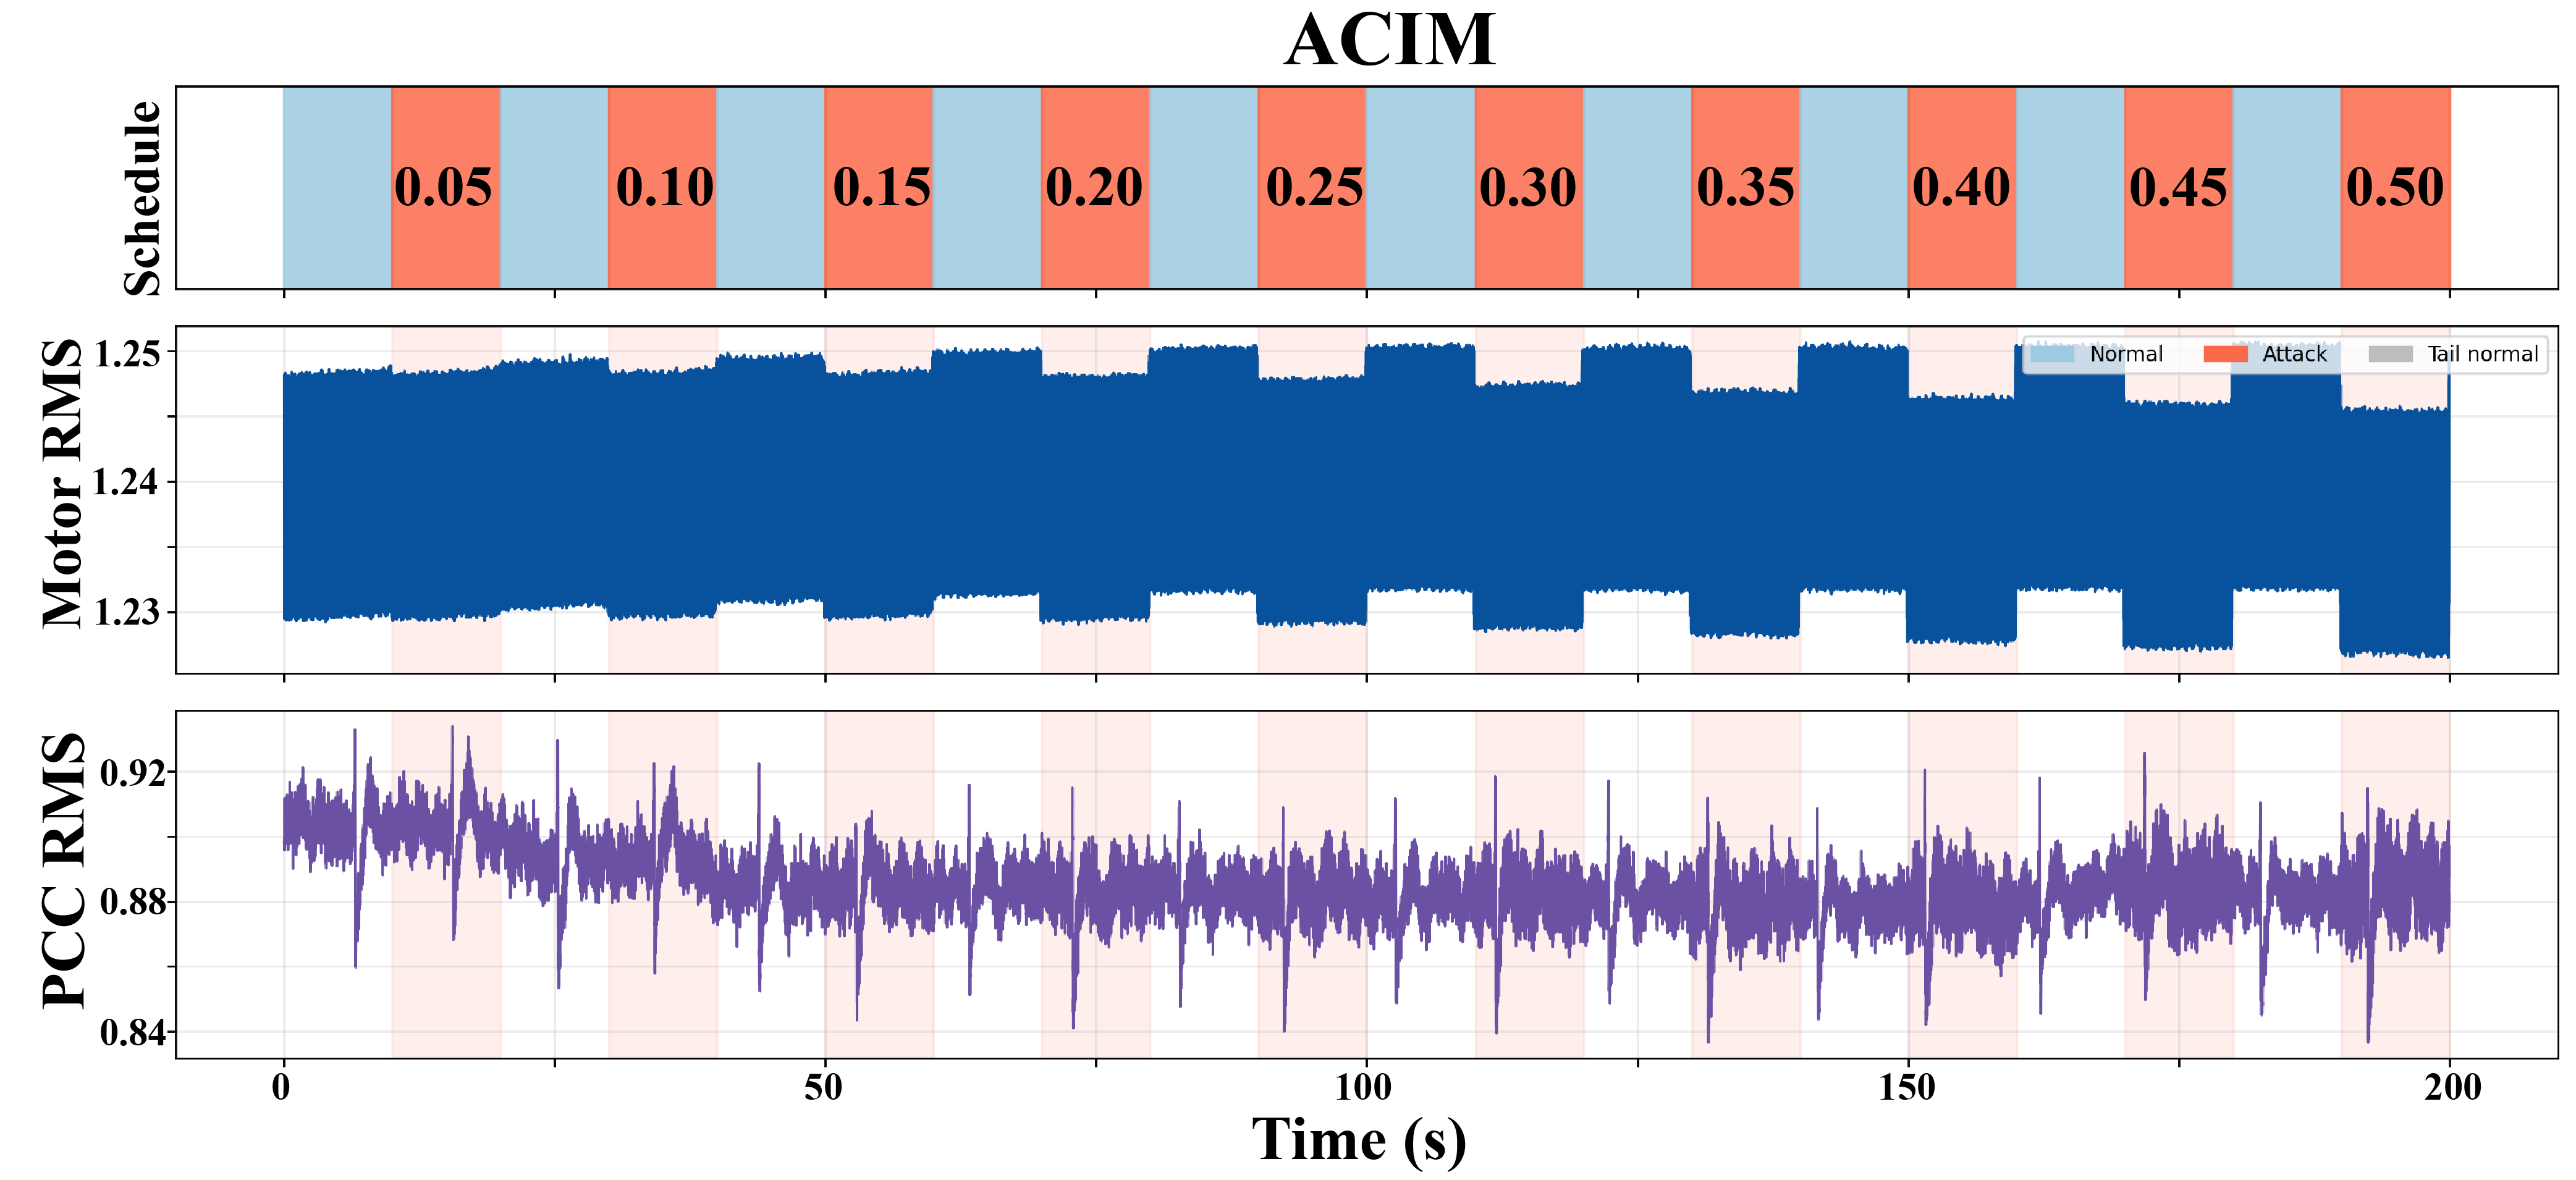
\includegraphics[width=0.49\textwidth]{figs/case1_30_motor_pcc_model_detection_200s_0p2s_rms61_continuous_rows124_revised.png}
    \hfill
    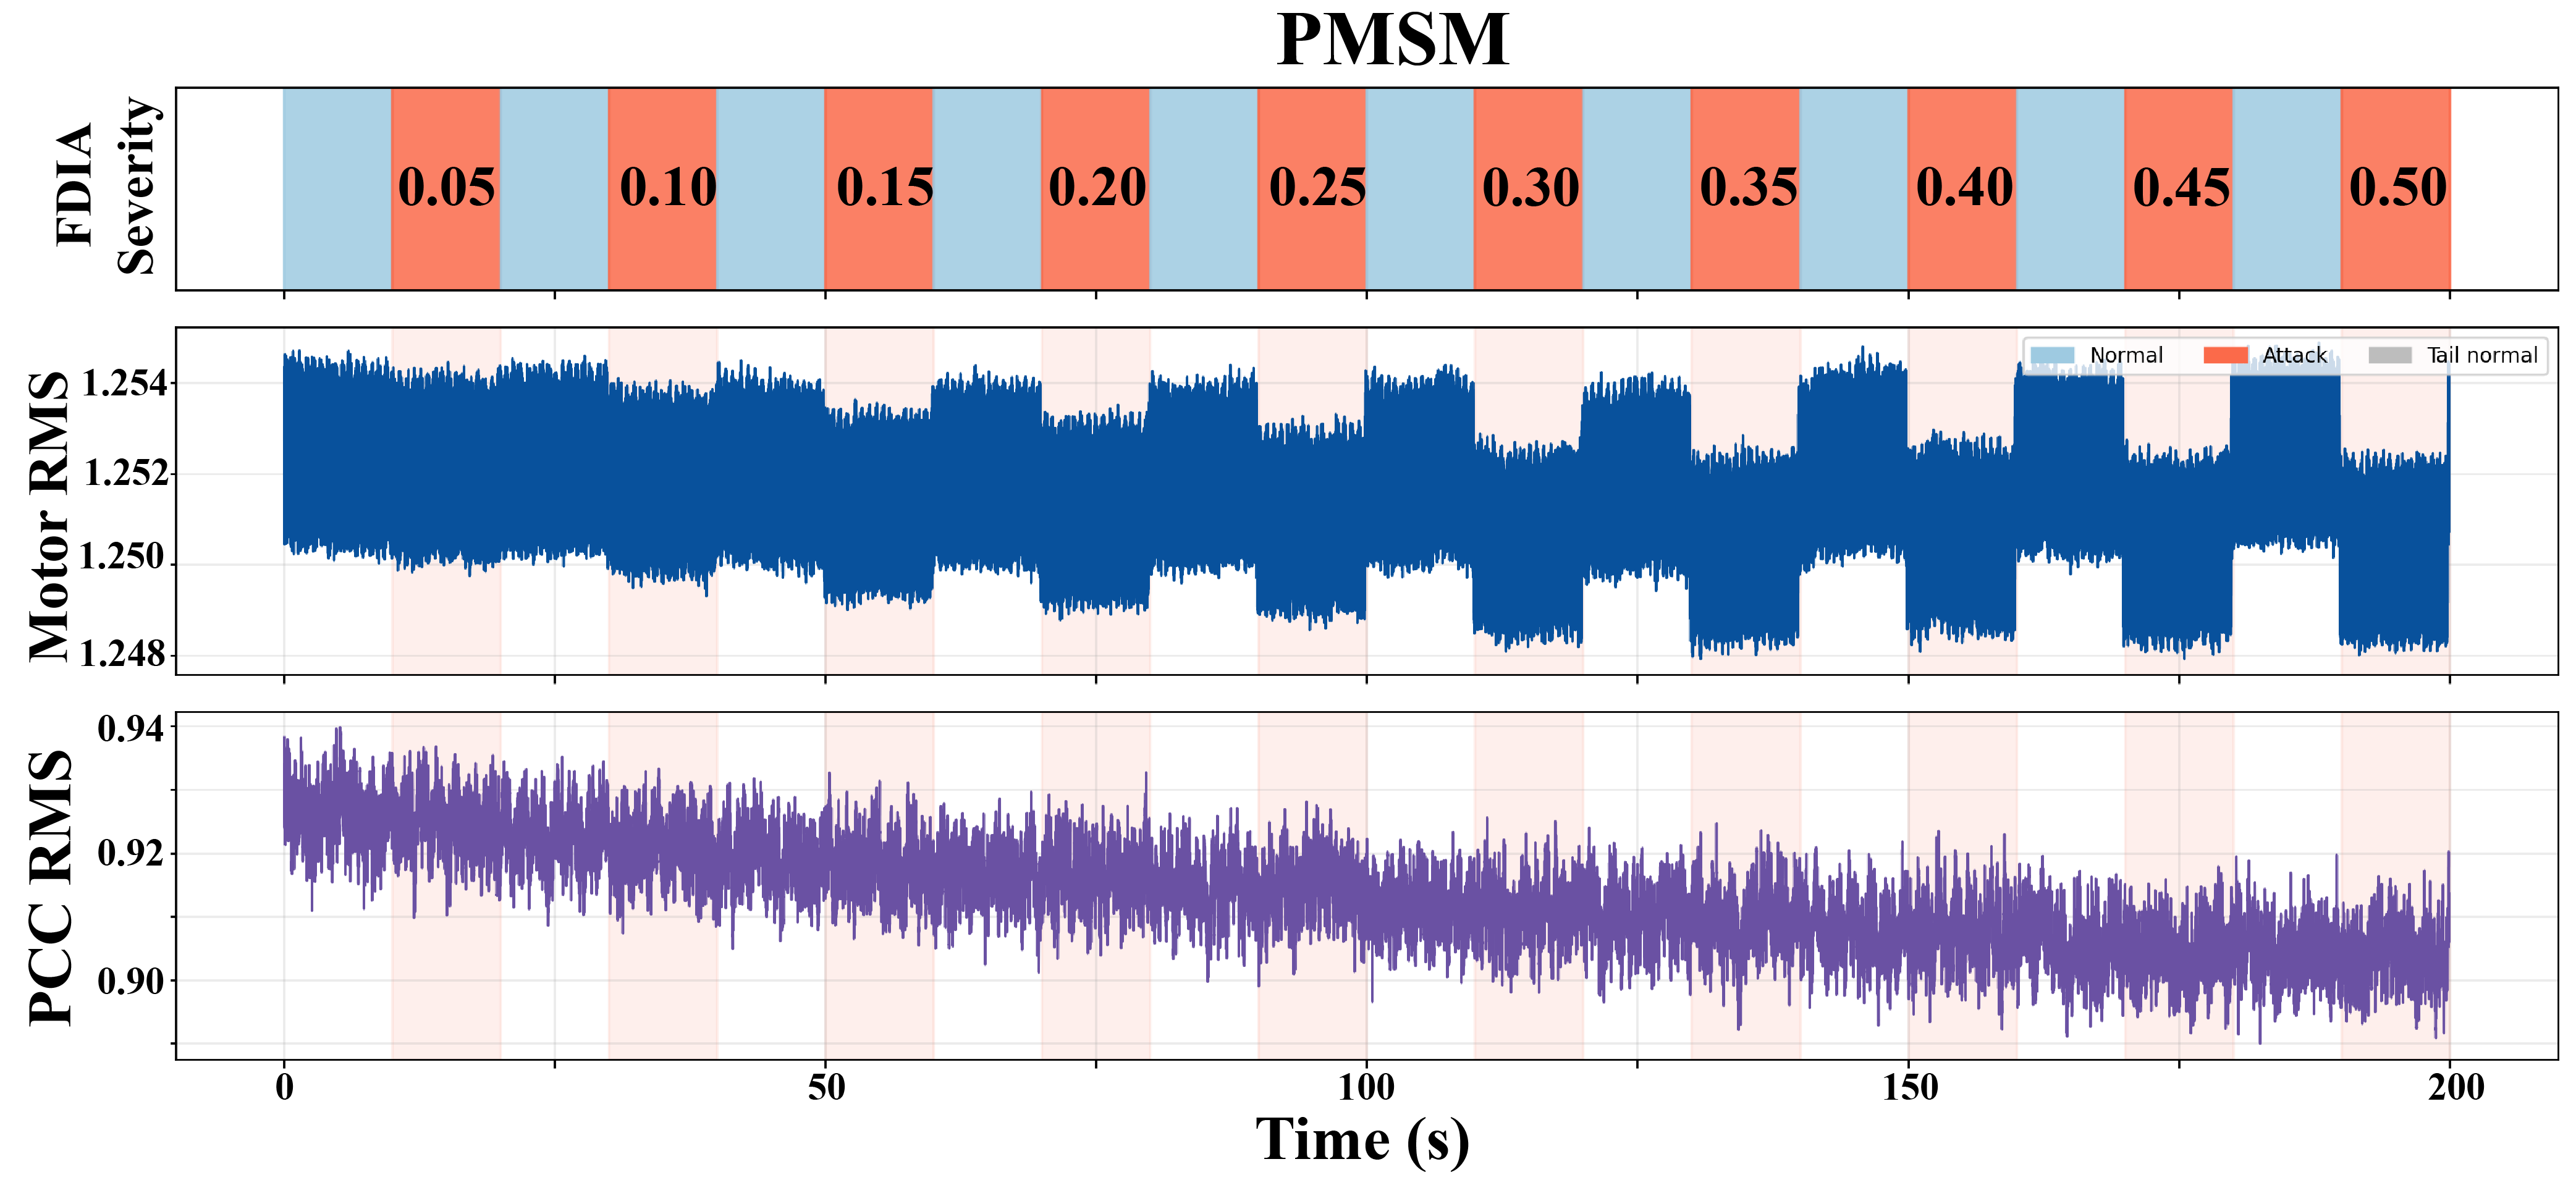
\includegraphics[width=0.49\textwidth]{figs/casepmsm271_300_motor_pcc_model_detection_200s_0p2s_rms61_continuous_rows124_revised.png}
    \DiffOriginalCaption{Figure 8: Representative consecutive FDIA episodes applied to the ACIM and PMSM motor-drive systems. Top: scheduled FDIA severity; middle: motor-current RMS; bottom: PCC-current RMS.}


\end{minipage}\par\vspace{1em}
% Complete new block: fig:app_attack_process_examples
\begin{minipage}[t]{\textwidth}
\centering
\textcolor{blue}{\textbf{REVISED --- Figure 9 (main\_revised.tex)}}\par\smallskip

\centering
\begingroup
\setlength{\unitlength}{1bp}
\resizebox{\linewidth}{!}{\begin{picture}(515.5200,161.0000)
\put(144.8379,153.0000){\makebox(0,0){\color[rgb]{0,0,0}\fontsize{10bp}{11bp}\selectfont ACIM}}
\put(43.9276,126.0000){\color[rgb]{0.665,0.809,0.887}\rule{10.0910bp}{9.0000bp}}
\put(54.0186,126.0000){\color[rgb]{0.986,0.489,0.375}\rule{10.0910bp}{9.0000bp}}
\put(59.0641,142.0000){\makebox(0,0){\color[rgb]{0,0,0}\fontsize{9.5bp}{10.5bp}\selectfont 0.05}}
\put(64.1096,126.0000){\color[rgb]{0.665,0.809,0.887}\rule{10.0910bp}{9.0000bp}}
\put(74.2007,126.0000){\color[rgb]{0.986,0.489,0.375}\rule{10.0910bp}{9.0000bp}}
\put(79.2462,142.0000){\makebox(0,0){\color[rgb]{0,0,0}\fontsize{9.5bp}{10.5bp}\selectfont 0.10}}
\put(84.2917,126.0000){\color[rgb]{0.665,0.809,0.887}\rule{10.0910bp}{9.0000bp}}
\put(94.3827,126.0000){\color[rgb]{0.986,0.489,0.375}\rule{10.0910bp}{9.0000bp}}
\put(99.4282,142.0000){\makebox(0,0){\color[rgb]{0,0,0}\fontsize{9.5bp}{10.5bp}\selectfont 0.15}}
\put(104.4737,126.0000){\color[rgb]{0.665,0.809,0.887}\rule{10.0910bp}{9.0000bp}}
\put(114.5648,126.0000){\color[rgb]{0.986,0.489,0.375}\rule{10.0910bp}{9.0000bp}}
\put(119.6103,142.0000){\makebox(0,0){\color[rgb]{0,0,0}\fontsize{9.5bp}{10.5bp}\selectfont 0.20}}
\put(124.6558,126.0000){\color[rgb]{0.665,0.809,0.887}\rule{10.0910bp}{9.0000bp}}
\put(134.7468,126.0000){\color[rgb]{0.986,0.489,0.375}\rule{10.0910bp}{9.0000bp}}
\put(139.7923,142.0000){\makebox(0,0){\color[rgb]{0,0,0}\fontsize{9.5bp}{10.5bp}\selectfont 0.25}}
\put(144.8379,126.0000){\color[rgb]{0.665,0.809,0.887}\rule{10.0910bp}{9.0000bp}}
\put(154.9289,126.0000){\color[rgb]{0.986,0.489,0.375}\rule{10.0910bp}{9.0000bp}}
\put(159.9744,142.0000){\makebox(0,0){\color[rgb]{0,0,0}\fontsize{9.5bp}{10.5bp}\selectfont 0.30}}
\put(165.0199,126.0000){\color[rgb]{0.665,0.809,0.887}\rule{10.0910bp}{9.0000bp}}
\put(175.1109,126.0000){\color[rgb]{0.986,0.489,0.375}\rule{10.0910bp}{9.0000bp}}
\put(180.1564,142.0000){\makebox(0,0){\color[rgb]{0,0,0}\fontsize{9.5bp}{10.5bp}\selectfont 0.35}}
\put(185.2020,126.0000){\color[rgb]{0.665,0.809,0.887}\rule{10.0910bp}{9.0000bp}}
\put(195.2930,126.0000){\color[rgb]{0.986,0.489,0.375}\rule{10.0910bp}{9.0000bp}}
\put(200.3385,142.0000){\makebox(0,0){\color[rgb]{0,0,0}\fontsize{9.5bp}{10.5bp}\selectfont 0.40}}
\put(205.3840,126.0000){\color[rgb]{0.665,0.809,0.887}\rule{10.0910bp}{9.0000bp}}
\put(215.4751,126.0000){\color[rgb]{0.986,0.489,0.375}\rule{10.0910bp}{9.0000bp}}
\put(220.5206,142.0000){\makebox(0,0){\color[rgb]{0,0,0}\fontsize{9.5bp}{10.5bp}\selectfont 0.45}}
\put(225.5661,126.0000){\color[rgb]{0.665,0.809,0.887}\rule{10.0910bp}{9.0000bp}}
\put(235.6571,126.0000){\color[rgb]{0.986,0.489,0.375}\rule{10.0910bp}{9.0000bp}}
\put(240.7026,142.0000){\makebox(0,0){\color[rgb]{0,0,0}\fontsize{9.5bp}{10.5bp}\selectfont 0.50}}
\put(37.9276,130.5000){\makebox(0,0)[r]{\color[rgb]{0,0,0}\fontsize{9.5bp}{10.5bp}\selectfont Bias (\%)}}
\put(43.92758,75){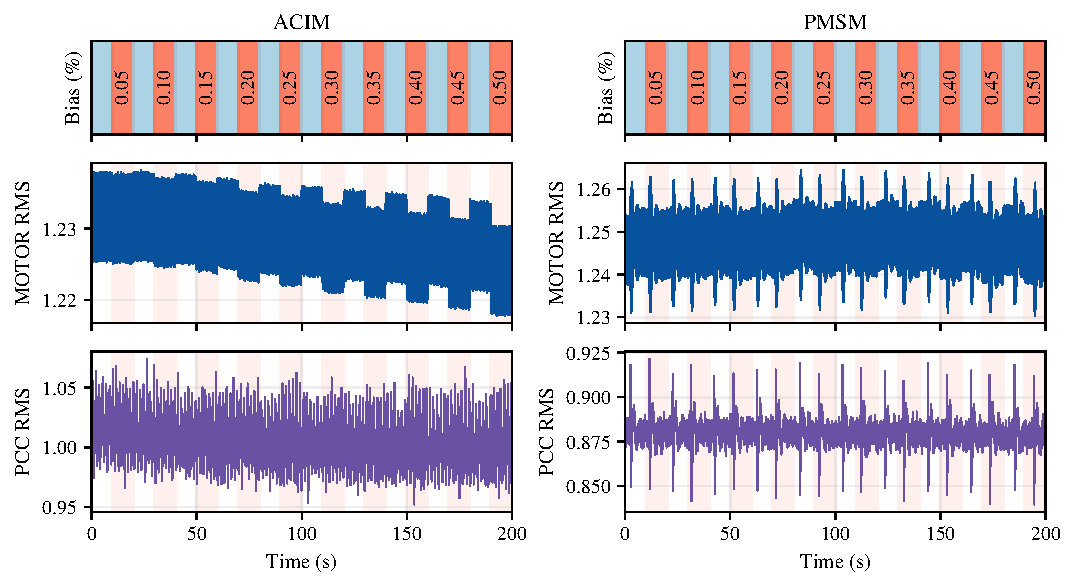
\includegraphics[viewport=43.92758 125.67077 245.74813 202.66817,clip,width=201.82055bp,height=44bp]{figs_revised/figure8_original_style.pdf}}
\put(38.9276,81.3454){\makebox(0,0)[r]{\color[rgb]{0,0,0}\fontsize{9.5bp}{10.5bp}\selectfont 1.22}}
\put(38.9276,100.9156){\makebox(0,0)[r]{\color[rgb]{0,0,0}\fontsize{9.5bp}{10.5bp}\selectfont 1.23}}
\put(6.9276,97.0000){\makebox(0,0){\rotatebox{90}{\color[rgb]{0,0,0}\fontsize{9.5bp}{10.5bp}\selectfont Motor RMS}}}
\put(43.92758,24){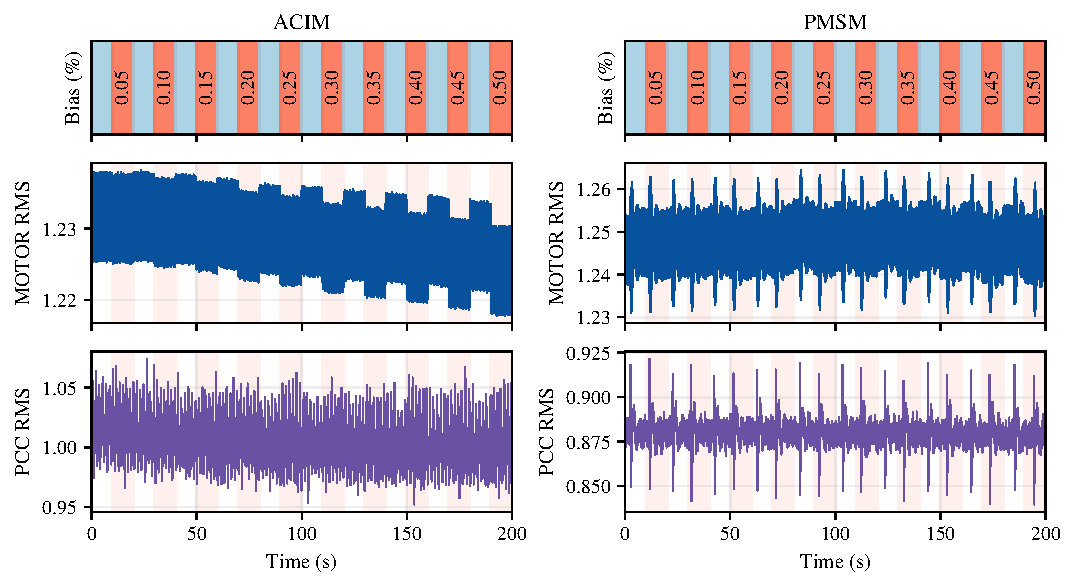
\includegraphics[viewport=43.92758 35.17252 245.74813 112.16993,clip,width=201.82055bp,height=44bp]{figs_revised/figure8_original_style.pdf}}
\put(38.9276,25.2713){\makebox(0,0)[r]{\color[rgb]{0,0,0}\fontsize{9.5bp}{10.5bp}\selectfont 0.95}}
\put(38.9276,41.6711){\makebox(0,0)[r]{\color[rgb]{0,0,0}\fontsize{9.5bp}{10.5bp}\selectfont 1.00}}
\put(38.9276,58.0708){\makebox(0,0)[r]{\color[rgb]{0,0,0}\fontsize{9.5bp}{10.5bp}\selectfont 1.05}}
\put(6.9276,46.0000){\makebox(0,0){\rotatebox{90}{\color[rgb]{0,0,0}\fontsize{9.5bp}{10.5bp}\selectfont PCC RMS}}}
\put(43.9276,15.0000){\makebox(0,0){\color[rgb]{0,0,0}\fontsize{9.5bp}{10.5bp}\selectfont 0}}
\put(94.3827,15.0000){\makebox(0,0){\color[rgb]{0,0,0}\fontsize{9.5bp}{10.5bp}\selectfont 50}}
\put(144.8379,15.0000){\makebox(0,0){\color[rgb]{0,0,0}\fontsize{9.5bp}{10.5bp}\selectfont 100}}
\put(195.2930,15.0000){\makebox(0,0){\color[rgb]{0,0,0}\fontsize{9.5bp}{10.5bp}\selectfont 150}}
\put(245.7481,15.0000){\makebox(0,0){\color[rgb]{0,0,0}\fontsize{9.5bp}{10.5bp}\selectfont 200}}
\put(144.8379,3.0000){\makebox(0,0){\color[rgb]{0,0,0}\fontsize{9.5bp}{10.5bp}\selectfont Time (s)}}
\put(400.9863,153.0000){\makebox(0,0){\color[rgb]{0,0,0}\fontsize{10bp}{11bp}\selectfont PMSM}}
\put(300.0760,126.0000){\color[rgb]{0.665,0.809,0.887}\rule{10.0910bp}{9.0000bp}}
\put(310.1670,126.0000){\color[rgb]{0.986,0.489,0.375}\rule{10.0910bp}{9.0000bp}}
\put(315.2125,142.0000){\makebox(0,0){\color[rgb]{0,0,0}\fontsize{9.5bp}{10.5bp}\selectfont 0.05}}
\put(320.2581,126.0000){\color[rgb]{0.665,0.809,0.887}\rule{10.0910bp}{9.0000bp}}
\put(330.3491,126.0000){\color[rgb]{0.986,0.489,0.375}\rule{10.0910bp}{9.0000bp}}
\put(335.3946,142.0000){\makebox(0,0){\color[rgb]{0,0,0}\fontsize{9.5bp}{10.5bp}\selectfont 0.10}}
\put(340.4401,126.0000){\color[rgb]{0.665,0.809,0.887}\rule{10.0910bp}{9.0000bp}}
\put(350.5312,126.0000){\color[rgb]{0.986,0.489,0.375}\rule{10.0910bp}{9.0000bp}}
\put(355.5767,142.0000){\makebox(0,0){\color[rgb]{0,0,0}\fontsize{9.5bp}{10.5bp}\selectfont 0.15}}
\put(360.6222,126.0000){\color[rgb]{0.665,0.809,0.887}\rule{10.0910bp}{9.0000bp}}
\put(370.7132,126.0000){\color[rgb]{0.986,0.489,0.375}\rule{10.0910bp}{9.0000bp}}
\put(375.7587,142.0000){\makebox(0,0){\color[rgb]{0,0,0}\fontsize{9.5bp}{10.5bp}\selectfont 0.20}}
\put(380.8042,126.0000){\color[rgb]{0.665,0.809,0.887}\rule{10.0910bp}{9.0000bp}}
\put(390.8953,126.0000){\color[rgb]{0.986,0.489,0.375}\rule{10.0910bp}{9.0000bp}}
\put(395.9408,142.0000){\makebox(0,0){\color[rgb]{0,0,0}\fontsize{9.5bp}{10.5bp}\selectfont 0.25}}
\put(400.9863,126.0000){\color[rgb]{0.665,0.809,0.887}\rule{10.0910bp}{9.0000bp}}
\put(411.0773,126.0000){\color[rgb]{0.986,0.489,0.375}\rule{10.0910bp}{9.0000bp}}
\put(416.1228,142.0000){\makebox(0,0){\color[rgb]{0,0,0}\fontsize{9.5bp}{10.5bp}\selectfont 0.30}}
\put(421.1683,126.0000){\color[rgb]{0.665,0.809,0.887}\rule{10.0910bp}{9.0000bp}}
\put(431.2594,126.0000){\color[rgb]{0.986,0.489,0.375}\rule{10.0910bp}{9.0000bp}}
\put(436.3049,142.0000){\makebox(0,0){\color[rgb]{0,0,0}\fontsize{9.5bp}{10.5bp}\selectfont 0.35}}
\put(441.3504,126.0000){\color[rgb]{0.665,0.809,0.887}\rule{10.0910bp}{9.0000bp}}
\put(451.4414,126.0000){\color[rgb]{0.986,0.489,0.375}\rule{10.0910bp}{9.0000bp}}
\put(456.4869,142.0000){\makebox(0,0){\color[rgb]{0,0,0}\fontsize{9.5bp}{10.5bp}\selectfont 0.40}}
\put(461.5325,126.0000){\color[rgb]{0.665,0.809,0.887}\rule{10.0910bp}{9.0000bp}}
\put(471.6235,126.0000){\color[rgb]{0.986,0.489,0.375}\rule{10.0910bp}{9.0000bp}}
\put(476.6690,142.0000){\makebox(0,0){\color[rgb]{0,0,0}\fontsize{9.5bp}{10.5bp}\selectfont 0.45}}
\put(481.7145,126.0000){\color[rgb]{0.665,0.809,0.887}\rule{10.0910bp}{9.0000bp}}
\put(491.8055,126.0000){\color[rgb]{0.986,0.489,0.375}\rule{10.0910bp}{9.0000bp}}
\put(496.8510,142.0000){\makebox(0,0){\color[rgb]{0,0,0}\fontsize{9.5bp}{10.5bp}\selectfont 0.50}}
\put(294.0760,130.5000){\makebox(0,0)[r]{\color[rgb]{0,0,0}\fontsize{9.5bp}{10.5bp}\selectfont Bias (\%)}}
\put(300.07601,75){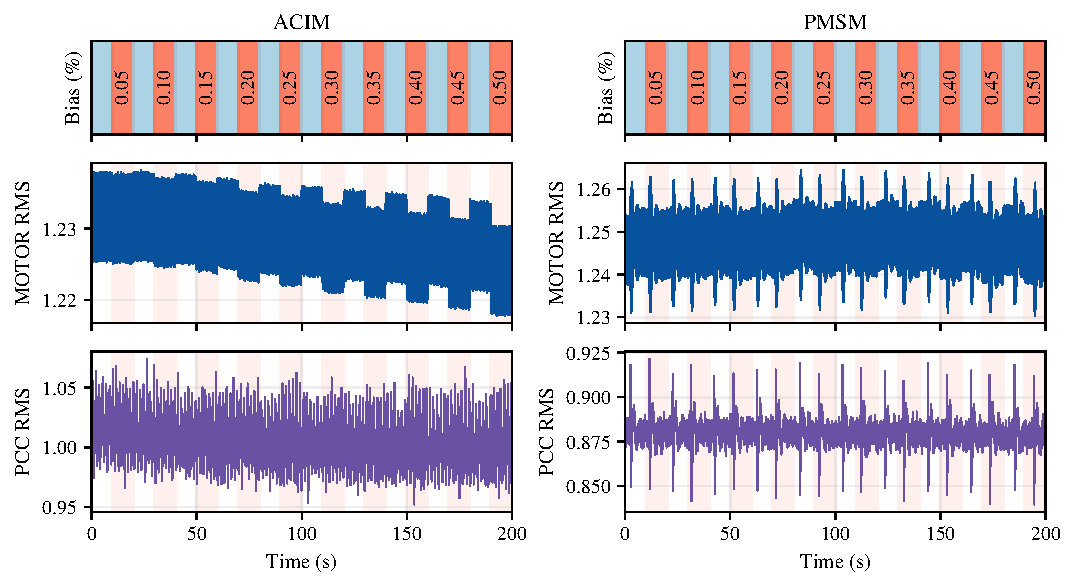
\includegraphics[viewport=300.07601 125.67077 501.89657 202.66817,clip,width=201.82055bp,height=44bp]{figs_revised/figure8_original_style.pdf}}
\put(295.0760,76.6377){\makebox(0,0)[r]{\color[rgb]{0,0,0}\fontsize{9.5bp}{10.5bp}\selectfont 1.23}}
\put(295.0760,88.3566){\makebox(0,0)[r]{\color[rgb]{0,0,0}\fontsize{9.5bp}{10.5bp}\selectfont 1.24}}
\put(295.0760,100.0733){\makebox(0,0)[r]{\color[rgb]{0,0,0}\fontsize{9.5bp}{10.5bp}\selectfont 1.25}}
\put(295.0760,111.7922){\makebox(0,0)[r]{\color[rgb]{0,0,0}\fontsize{9.5bp}{10.5bp}\selectfont 1.26}}
\put(263.0760,97.0000){\makebox(0,0){\rotatebox{90}{\color[rgb]{0,0,0}\fontsize{9.5bp}{10.5bp}\selectfont Motor RMS}}}
\put(300.07601,24){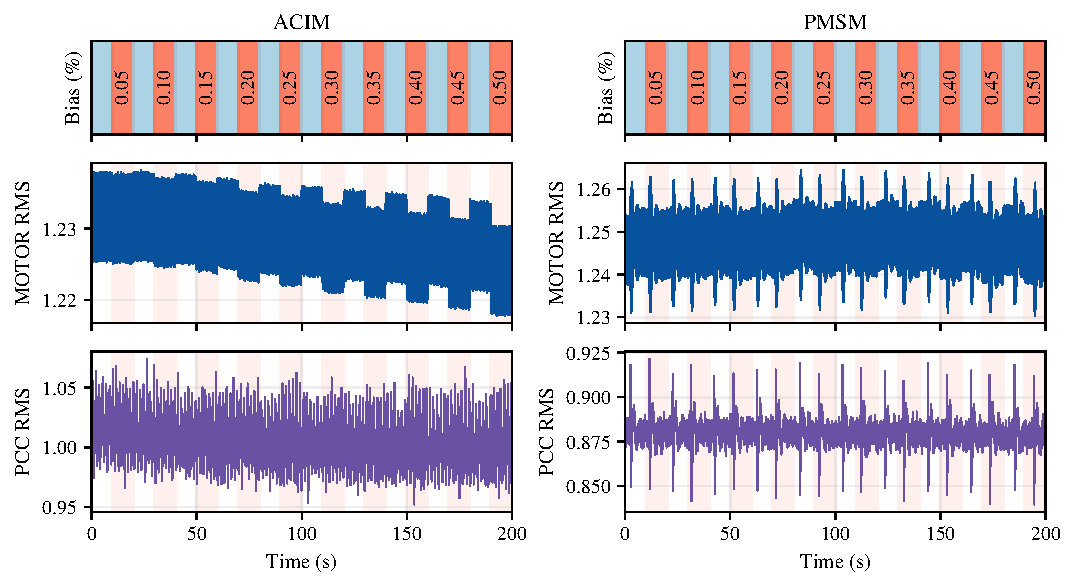
\includegraphics[viewport=300.07601 35.17252 501.89657 112.16993,clip,width=201.82055bp,height=44bp]{figs_revised/figure8_original_style.pdf}}
\put(295.0760,31.0157){\makebox(0,0)[r]{\color[rgb]{0,0,0}\fontsize{9.5bp}{10.5bp}\selectfont 0.850}}
\put(295.0760,43.2172){\makebox(0,0)[r]{\color[rgb]{0,0,0}\fontsize{9.5bp}{10.5bp}\selectfont 0.875}}
\put(295.0760,55.4164){\makebox(0,0)[r]{\color[rgb]{0,0,0}\fontsize{9.5bp}{10.5bp}\selectfont 0.900}}
\put(295.0760,67.6179){\makebox(0,0)[r]{\color[rgb]{0,0,0}\fontsize{9.5bp}{10.5bp}\selectfont 0.925}}
\put(263.0760,46.0000){\makebox(0,0){\rotatebox{90}{\color[rgb]{0,0,0}\fontsize{9.5bp}{10.5bp}\selectfont PCC RMS}}}
\put(300.0760,15.0000){\makebox(0,0){\color[rgb]{0,0,0}\fontsize{9.5bp}{10.5bp}\selectfont 0}}
\put(350.5312,15.0000){\makebox(0,0){\color[rgb]{0,0,0}\fontsize{9.5bp}{10.5bp}\selectfont 50}}
\put(400.9863,15.0000){\makebox(0,0){\color[rgb]{0,0,0}\fontsize{9.5bp}{10.5bp}\selectfont 100}}
\put(451.4414,15.0000){\makebox(0,0){\color[rgb]{0,0,0}\fontsize{9.5bp}{10.5bp}\selectfont 150}}
\put(501.8966,15.0000){\makebox(0,0){\color[rgb]{0,0,0}\fontsize{9.5bp}{10.5bp}\selectfont 200}}
\put(400.9863,3.0000){\makebox(0,0){\color[rgb]{0,0,0}\fontsize{9.5bp}{10.5bp}\selectfont Time (s)}}
\end{picture}}
\endgroup
\caption{Representative ACIM/PMSM attack episodes: injected bias (top), motor-current RMS (middle), and PCC-current RMS (bottom), in acquisition units.}
\label{fig:app_attack_process_examples}

\end{minipage}
\end{minipage}
\end{adjustbox}
\end{figure*}





\DIFaddend \subsection{Extracted Feature Set}
\label{app:feature_set}

Table~\ref{tab:app_extracted_features} summarizes the extracted features used in the proposed LF/HF/TD pipeline. Each channel is represented using low-frequency spectral features, high-frequency spectral-envelope features, and time-domain statistical features.
\DIFaddbegin



\begin{table*}[p]
\centering
\begin{adjustbox}{max width=\textwidth,max totalheight=0.87\textheight}
\begin{minipage}{\textwidth}
\centering
% Complete old block: tab:app_extracted_features
\begin{minipage}[t]{0.48\textwidth}
\centering
\textcolor{red}{\textbf{ORIGINAL --- Table 12 (main.tex)}}\par\smallskip

\centering
\scriptsize
\DiffOriginalCaption{Table 12: Extracted features per channel in the proposed LF/HF/TD pipeline.}

\setlength{\tabcolsep}{3pt}
\renewcommand{\arraystretch}{1.08}
\begin{adjustbox}{max width=\linewidth}\begin{tabularx}{\columnwidth}{l c c X}
\hline
Type & No. & Window / Stride & Features \\
\hline
LF & 18 & 500 / 25 &
$A_1$, $f_1$, $\phi_1$, THD, $H_2/H_1$, $H_3/H_1$, $H_5/H_1$, $H_7/H_1$,
$\phi_3-\phi_1$, $\phi_5-\phi_1$, sideband energy/ratio,
$E_{0-120}$, $E_{120-300}$, $E_{300-500}$,
$df_1/dt$, $dA_1/dt$, $d\mathrm{THD}/dt$ \\
\hline
HF & 11 & 500 / 25 &
RMS$_{2-5k}$, energy ratio, centroid, bandwidth, flatness, kurtosis,
peak frequency, peak-to-band, envelope RMS, envelope kurtosis, envelope crest factor \\
\hline
TD & 8 & 500 / 25 &
RMS, standard deviation, crest factor, kurtosis, skewness, peak-to-peak, line length, Teager MAV \\
\hline
Total & 37 & -- & LF (18), HF (11), TD (8) \\
\hline
\end{tabularx}\end{adjustbox}

\end{minipage}\hfill%
% Complete new block: tab:app_extracted_features
\begin{minipage}[t]{0.48\textwidth}
\centering
\textcolor{blue}{\textbf{REVISED --- Table 12 (main\_revised.tex)}}\par\smallskip

\centering
\scriptsize
\caption{Extracted features per channel in the proposed LF/HF/TD pipeline.}
\label{tab:app_extracted_features}
\setlength{\tabcolsep}{3pt}
\renewcommand{\arraystretch}{1.08}
\begin{tabularx}{\columnwidth}{l c c X}
\hline
Type & No. & \shortstack{Window / Stride\\(samples)} & Features \\
\hline
LF & 18 & 500 / 25 &
$A_1$, $f_1$, $\phi_1$, THD, $H_2/H_1$, $H_3/H_1$, $H_5/H_1$, $H_7/H_1$,
$\phi_3-\phi_1$, $\phi_5-\phi_1$, sideband energy/ratio,
$E_{0-120}$, $E_{120-300}$, $E_{300-500}$,
$df_1/dt$, $dA_1/dt$, $d\mathrm{THD}/dt$ \\
\hline
HF & 11 & 250 / 29 &
$\mathrm{RMS}_{2\text{--}5\,\mathrm{kHz}}$, energy ratio, centroid, bandwidth, flatness, kurtosis,
peak frequency, peak-to-band, envelope RMS, envelope kurtosis, envelope crest factor \\
\hline
TD & 8 & 500 / 25 &
RMS, standard deviation, crest factor, kurtosis, skewness, peak-to-peak, line length, Teager MAV \\
\hline
Total & 37 & -- & LF (18), HF (11), TD (8) \\
\hline
\end{tabularx}
\par\smallskip\raggedright
THD: total harmonic distortion; MAV: mean absolute value. Subscripts of $E$ give frequency-band limits in hertz.

\end{minipage}
\end{minipage}
\end{adjustbox}
\end{table*}





\subsection{\DIFadd{Severity-Conditioned Attack Detection}}
\label{app:severity_detection}
\DIFadd{Table~\ref{tab:severity_detection_recall} separates correct bias-bin classification from detecting any attack. For confusion matrix $C$, severity-conditioned attack recall is
}\begin{equation}
\DIFadd{R_{\mathrm{attack}|k}=\frac{\sum_{j=1}^{3}C_{kj}}{\sum_{j=0}^{3}C_{kj}},\qquad k\in\{1,2,3\},
\label{eq:severity_conditioned_detection}
}\end{equation}
\DIFadd{while exact-severity recall is $C_{kk}/\sum_j C_{kj}$. The repeated false-alarm entries belong to the same four-class model and do not depend on the actual attack level. Fig.~\ref{fig:severity_detection_decisions}(c), (d) presents the corresponding PCC decision matrices; pooled normal recall can differ slightly from the mean per-repeat recall because normal-window counts vary across holdouts.
}



\begin{table*}[p]
\centering
\begin{adjustbox}{max width=\textwidth,max totalheight=0.87\textheight}
\begin{minipage}{\textwidth}
\centering
% Complete new block: tab:severity_detection_recall
\begin{minipage}[t]{\DiffColumnWidth}
\centering
\textcolor{blue}{\textbf{REVISED --- Table 13 (main\_revised.tex)}}\par\smallskip

\centering
\footnotesize
\caption{Exact-severity and any-attack recall from four-class predictions (\%).}
\label{tab:severity_detection_recall}
\renewcommand{\arraystretch}{1.15}
\setlength{\tabcolsep}{2.2pt}
\begin{tabular}{@{}lccc@{}}
\hline
True bias & \shortstack{Exact\\recall} & \shortstack{Any-attack\\recall} & \shortstack{Normal false\\alarms} \\\hline
\hline\multicolumn{4}{c}{\textit{MOTOR stream}} \\\hline
Low & \mbox{89.58\,$\pm$\,2.14} & \mbox{95.58\,$\pm$\,4.15} & \mbox{19.08\,$\pm$\,16.08} \\
Medium & \mbox{93.96\,$\pm$\,1.05} & \mbox{99.71\,$\pm$\,0.04} & \mbox{19.08\,$\pm$\,16.08} \\
High & \mbox{98.76\,$\pm$\,0.27} & \mbox{99.65\,$\pm$\,0.29} & \mbox{19.08\,$\pm$\,16.08} \\
\hline\multicolumn{4}{c}{\textit{PCC stream}} \\\hline
Low & \mbox{38.33\,$\pm$\,7.04} & \mbox{61.39\,$\pm$\,2.64} & \mbox{37.23\,$\pm$\,3.17} \\
Medium & \mbox{50.58\,$\pm$\,7.01} & \mbox{85.08\,$\pm$\,6.52} & \mbox{37.23\,$\pm$\,3.17} \\
High & \mbox{70.79\,$\pm$\,2.28} & \mbox{88.09\,$\pm$\,7.22} & \mbox{37.23\,$\pm$\,3.17} \\
\hline\end{tabular}
\par\smallskip\begin{minipage}{\columnwidth}\scriptsize Mean $\pm$ sample SD over three holdouts. False alarms refer to the same normal class for all three attack levels. Different metrics are not competing methods, so none is highlighted as best.\end{minipage}

\end{minipage}
\end{minipage}
\end{adjustbox}
\end{table*}
\DIFaddend



\end{document}
